\documentclass[twoside]{report}




% Load the packages

%\usepackage[latin1]{inputenc}
\usepackage[utf8]{inputenc}
%\usepackage[french]{babel}
\usepackage[T1]{fontenc}
\usepackage{amsmath}
%\usepackage{amsfonts}
\usepackage{amssymb} % for the checkmark
\usepackage{makeidx}
\usepackage{graphicx}
\usepackage{lmodern}
\usepackage[left=2.5cm,right=2.5cm,top=2cm,bottom=2cm]{geometry}  % marges
\usepackage{color}
\usepackage{xcolor}
\setcounter{secnumdepth}{4} % augmentation de la num?rotation des sous-sections
\setcounter{tocdepth}{3} % augmentation de la profondeur de la table des mati?res

%\setlength{\parindent}{0cm} %Para las sangrias

% Ce package je ne sais pas pour qu'il soit utilisé
\usepackage{titlesec}

% Ce package est pour plusiers rangées
\usepackage{multirow}

% Ce package est pour la représentation des molécules. Il a besoin de chemist.sty et assurechemist.sty
\usepackage{chemist}

% Ce package est pour la représentation des nombres et des unités de mesure
%\usepackage{si}

\usepackage{svg}

\usepackage{bm}

% Ce package est pour écrire les références avec natbit dans le Harvard style
%\usepackage{natbib}
%\addbibresource{files/bibliographyFile.bib}


% Ce package est pour écrire les références avec biblatex: biblatex.sty, etoolbox.sty, logreq.sty, logreq.def, url.sty
%\usepackage{biblatex}
%\usepackage{cite}
%\addbibresource{bibliographyFile.bib}
%\DeclareNameAlias{sortname}{family-given}
%\DeclareNameAlias{default}{family-given}

% Ce package fait que les phrases ou expressions changent de ligne
\usepackage{makecell}

% Pour les hyperreferences
\usepackage[hidelinks]{hyperref}

% Pour changer l'orientation des foies
\usepackage{pdflscape}
\usepackage{lscape}
%\usepackage[paper=portrait,pagesize]{typearea} % Careful! Changes all the document into portrait mode!

% Pour emphatiser des equations (tables ...)
%\usepackage{empheq}

% Pour changer localement les margins
\usepackage{changepage}

%%%%%%%%%%%%%%%%%%%%%%%%%%%% Pour la bibliographie %%%%%%%%%%%%%%%%%%%%%%%%%%%%%%%

% Bibliographie avec natbib:
\usepackage{natbib}
\bibliographystyle{agsm} %agsm, unsrtnat

\usepackage{subcaption}

%% Bibliographie avec biblatex
%\usepackage[backend=bibtex]{biblatex}
%\addbibresource{files/bibliographyFile.bib}
%\DeclareNameAlias{sortname}{family-given}
%\DeclareNameAlias{default}{family-given}

%%%%%%%%%%%%%%%%%%%%%%%%%%%%%%%%%%%%%%%%%%%%%%%%%%%%%%%%%%%%%%%%%%%%%%%%%%%%%%%%%%
\newcommand{\citepBlackColor}[1][]{({\color{black}\citealt{#1}})}
\newcommand{\citeWhiteColor}[1][]{{\color{white}\cite{#1}}}
\newcommand{\citeColor}[1][]{{\color{blue}\cite{#1}}}
\newcommand{\citepColor}[1][]{({\color{blue}\citealt{#1}})}
\newcommand{\citemColor}[1][]{({\color{blue}\citealt{#1}})}

\newcommand{\introductoryParagraph}[1]{%
\begin{adjustwidth}{1in}{1in}
\textsl{#1}
\end{adjustwidth}
}

\usepackage{gensymb}

\usepackage{fancyhdr}

\usepackage{empheq}
\usepackage{relsize}

\usepackage{upgreek}

% For the diameter symbol
\usepackage{wasysym}

% PACKAGES TO ADD 
%\usepackage{enumitem}   % https://stackoverflow.com/questions/2007627/latex-how-can-i-create-nested-lists-which-look-this-1-1-1-1-1-1-1-2-1-2

\DeclareMathOperator\erf{erf}

%% NOMENCLATURE
% https://www.overleaf.com/learn/latex/nomenclatures
% https://tex.stackexchange.com/questions/112884/how-to-achieve-nomenclature-entries-like-symbol-description-dimension-and-uni
% https://www.youtube.com/watch?v=Ss1XfsaAnfs
% https://tex.stackexchange.com/questions/86666/how-to-create-both-list-of-abbreviations-and-list-of-nomenclature-using-nomencl/87223
\usepackage[intoc]{nomencl}
\makenomenclature

%% this modifies item separation:
\setlength{\nomitemsep}{12pt}

\usepackage{etoolbox}
\renewcommand\nomgroup[1]{%
  \item[\bfseries
  \ifstrequal{#1}{A}{Acronyms}{%
  \ifstrequal{#1}{D}{Dimensionless numbers}{
  \ifstrequal{#1}{G}{Greek Symbols}{%
  \ifstrequal{#1}{R}{Roman Symbols}{%
  \ifstrequal{#1}{Sb}{Subscripts}{%
  \ifstrequal{#1}{Sp}{Superscripts}{}}}}}}%
]}
%]\vspace{10pt}} % this is to add vertical space between the groups.

% This will add the units
%----------------------------------------------
\newcommand{\nomunit}[1]{%
\renewcommand{\nomentryend}{\hspace*{\fill}#1}}
%----------------------------------------------


%%%%% For appendices %%%%%
%\usepackage[toc,page]{appendix}
\usepackage[titletoc]{appendix} % Para apéndices: http://stackoverflow.com/questions/5690679/add-appendix-before-a-in-thesis-toc
\usepackage{chngcntr} %Para los apéndices: http://tex.stackexchange.com/questions/85776/change-figure-numbering-for-appendix

%%%%% Thick lines, ref: https://tex.stackexchange.com/questions/41758/how-can-i-reproduce-this-table-with-thick-lines
\makeatletter
\newcommand{\thickhline}{%
    \noalign {\ifnum 0=`}\fi \hrule height 1pt
    \futurelet \reserved@a \@xhline
}
\newcolumntype{"}{@{\hskip\tabcolsep\vrule width 1pt\hskip\tabcolsep}}
\makeatother


% Redefine paragraph command
\titleformat{\paragraph}
{\normalfont\normalsize\bfseries}{\theparagraph}{1em}{}
\titlespacing*{\paragraph}
{0pt}{3.25ex plus 1ex minus .2ex}{1.5ex plus .2ex}

% Cover: https://tlsflyleaf.onada.fr/
\usepackage[ED=MEGEP-Energ,Ets=INP]{tlsflyleaf}

% For highlighting
\usepackage{color,soul}


% Create commands
%\newcommand{\tab_space}{[0.3cm]}
\def \tab_space {\\[0.2cm]}

% 
\usepackage{array,booktabs}


% Greek letters inkscape:
% http://kestrel.nmt.edu/~raymond/software/howtos/greekscape.xhtml

% Headers and footers
\renewcommand{\chaptermark}[1]{\markboth{\chaptername\ \thechapter.\ #1}{}}
\renewcommand{\sectionmark}[1]{\markright{\thesection.\ #1}}

\pagestyle{fancy}
\fancyhead[LE]{\leftmark}
\fancyhead[RE]{}
\fancyhead[LO]{}
%\fancyhead[RO]{Guides and tutorials}
\fancyfoot[CE,CO]{\thepage}



% volume fraction reference in document:
% \ref{eq:vol_frac_definition}

\begin{document}


% Portada:
% https://tlsflyleaf.onada.fr/

% Include the cover
% My cover
\begin{titlepage}
	\setlength{\unitlength}{1 cm} %Especificar unidad de trabajo
\thispagestyle{empty}




~ ~

\vspace{5.5cm}
  
\begin{center}

\Huge \textbf{Modeling of Multipoint Fuel Injection for the Large Eddy Simulation of Aeronautical Combustion Chambers}

%\noindent\rule{\textwidth}{0.4pt}


\vspace{10.5cm}

{\LARGE \textbf{Carlos G. Guillam\'on}}\\[1cm]
\end{center}

%\begin{center}
%	Last revision: \today
%\end{center}





\end{titlepage}

%%%% Toulouse Cover %%%%%%%%%%% https://tlsflyleaf.onada.fr/
%
\title{Modeling of Multipoint Fuel Injection for the Large Eddy Simulation of Aeronautical Combustion Chambers}
\author{Carlos GARCIA GUILLAMON}
\defencedate{Date de défense (JJ/MM/AAAA)}
\lab{CERFACS}
%\cotutelle{Institut de cotutelle}

%% Directeur(s) de thèse
\nboss{2}                                    % Nombre de directeur(s) de thèse
\makesomeone{boss}{2}{Second DIRECTEUR}{}{}  % Sera affiché en second
\makesomeone{boss}{1}{Premier DIRECTEUR}{}{} % Sera affiché en premier
%% Referee
\nreferee{2}
\makesomeone{referee}{1}{Premier RAPPORTEUR}{}{}
\makesomeone{referee}{2}{Second RAPPORTEUR}{}{}
%% Jury
\njudge{3}
\makesomeone{judge}{1}{Premier MEMBRE}{Professeur d'Université}{Président du Jury}
\makesomeone{judge}{2}{Second MEMBRE}{Astronome Adjoint}{Membre du Jury}
\makesomeone{judge}{3}{Troisième MEMBRE}{Chargé de Recherche}{Membre du Jury}

\makeflyleaf




%%%%%%%%%%%%%%%%%%%%%%%%%%%%%%%

\pagenumbering{roman}
\newpage

%\shipout\null % Blank page 
%\stepcounter{page}
%\newpage
%\setcounter{page}{3}
%\thispagestyle{empty}

\vspace*{\fill}
%\vspace*{1.5in}
\begin{flushleft}
%\textit{Échale valor, que no vivan por ti. \\
%Y si no ves salida lárgate de allí.}\\
\textit{Y si fuera \\
mi vida una escalera \\
me la he pasado entera \\
buscando el siguiente escal\'on} \\
\vspace{0.05in}
%Molly (Hamlet)
Robe
\end{flushleft}

\vspace*{\fill}
%\vspace*{0.5in}
\begin{flushright}
\textit{Parce que, dans le reste de la vie, \\
personne ne vous demande de chercher \\
quoi que ce soit,\\
et on ne risque pas de trouver\\
puisqu'on ne sait pas \\
ce qu'on cherche} \\
\vspace{0.05in}
Fred Vargas
\end{flushright}
\vspace*{\fill}



%\vspace{5in}


%\newpage

\shipout\null % Blank page
\stepcounter{page}
\tableofcontents
\newpage
\chapter*{Acknowledgements}
    \addcontentsline{toc}{chapter}{Acknowledgements}
    
Dans \textsl{Siddhartha} \citepColor[hesse_siddhartha_1922], le passeur de la rivière apprend au protagoniste comment croisser celle-ci. D'abord il lui aide à croisser et a entendre cette rivière, jusqu'au moment ou Siddhartha arrive à la traspasser lui même, apprendant à écouter le fleuve et comprenant son esprit. \\  % p. 115
%
Je remercie d'abord à mes deux passeurs, Léa Voivenel et Renaud Mercier, qui m'ont  à croisser et à entendre cette rivière qu'on appelle recherche. Ses conseils, son inestimable aide, sa constant disposition et sa patience m'ont permi d'aboutir ce projet qui a prit autant d'effort et de temps dans ma vie.

Je dois exprimer ma profonde gratitude à Thierry Poinsot pour diriger cette thèse et pour m'avoir accueilli au CERFACS pour les dernièrs mois de ma thèse. Je remercie vraiement le temps qu'il a pris, malgré son calendrier serré, pour assister aux réunions que m'ont permis d'ameliorer les modèles et les simulations.

Je souhaiterais aussi remercier aux membres du jury pour assister à ma soutenance. Merci à Aymeric Vié et Guillaume Balarac pour accepter d'ètre rapporteurs et pour prendre le temps de lire et évaluer ce manuscrit (qui n'est pas le roman le plus amusant du monde...).  Merci a François-Xavier Demoulin pour accepter de présider le jury, et à Jean-Luc Estivalèzes, Marcos Carreres, Vincent Moureau et Stefano Puggelli pour évaluer mon travail lors de la soutenance. Aussi, merci à Stefano et à Vincent pour nos discussions et ses conseils, à Safran ou en visio. 

Maintenant, je dois rendre grâce en faisant un petit \textsl{road trip} qui va du nord de France au plus sud, de Paris à l'Espagne. 

A Paris, je souheterais remercier d'abord les gens qui j'ai trouvés à Safran Tech, dans les pôles "Energie et Propulsion" et "Digital Sciences and Technologies". D'abord (et evidemment), merci encore une fois à Léa et à Renaud pour m'acueillir dans ses départements. Du còté technique, merci à Melody Cailler et à Julien Leparoux pour tous nos échanges et pour partager son expérience sur le diphasique et sur YALES2 avec moi.  Et du côté personnel, je ne peux que être reconnaissant d'avoir trouvé à des gens comme Romain Janodet, mon copain d'enjeux diphasiques et des hauts et bas de thêse (et avec qui j'espere pouvoir collaborer dans un avenir proche); Gabriel Mondin, compagne de bureau d'abord, puis pote d'aventures à Paris, Lyon et Barcelone (il nous manque Raz toujours!); Quentin Holka, le bon breton avec qui nous nous sommes appuyés pour sortir de l'abysme dans les moments les plus durs; Clement Pornet, le \textsl{loco} d'ouf qui a quitté l'endroit pour aller faire des avions (et qui m'a laissé tout seul dans la salle de sport); Jean-Marie Kai, le master versaillais (car lui, lui il est français) du control et du pilotage; et à Deepali Singh, qui a quitté la region parisienne trop tôt pour faire de l'eolienne chez les champs de tulipes néerlandais (now it's your turn to get that PhD, go kill it girl!).
  
\textbf{Paris (hors Safran}).  Toujours dans la capitale, la Ville Lumière n'aurait pas été aussi charmant sans la compagnie de quelques personnes.

In first place, I should start with the flashbacs in the CIUP, my first home in Paris.



\textbf{Toulouse}. 

\textbf{Barcelone}. Cruzando los Pirineos hacia el sur, me gustaría empezar por agradecer en Barcleona el apoyo moral a mis colegas del BSC y a mi familia de aquí, fundamental en este periodo de correcciones y lectura de tesis que se ha alargado más de lo previsto. 


\textbf{Valencia (mirlos)? Maybe not}


\textbf{Requena}


\textbf{Family}


\textbf{Laura}


\subsection*{Financement}

This PhD thesis has been funded by the European Union Horizon 2020 research and innovation program under the Marie Sklodowska-Curie grant agreement No. 765998 in the project ANNULIGhT. Computer resources provided by GENCI, France, under the allocations A0092B11072 and A0092B10157.

%NOTE: A0092B11072 corresponds to Safran Tech (Mélody), A0092B11072 to Cerfacs one (Florent/Eleonore)


%\newpage
%\shipout\null % Blank page
%\stepcounter{page}
%\newpage
%\thispagestyle{empty}

\vspace*{\fill}
\begin{flushright}
\textit{Las obras nunca se terminan. El truco est\'a en saber d\'onde hay que dejarlas inacabadas} \\
\vspace{0.05in}
Carlos Ruiz Zaf\'on
\end{flushright}
\vspace*{\fill}





\newpage
\shipout\null % Blank page
\stepcounter{page}
\newpage
%\chapter*{Nomenclature}
%    \addcontentsline{toc}{chapter}{Nomenclature}
    
% Compiling command (makeindex): 
% Without nomenclature: makeindex %.idx
% With nomenclature:  makeindex %.nlo -s nomencl.ist -o %.nls -t %.nlg   

    
% ACRONYMS
\nomenclature[A]{ALM}{Actuator Line Method}
\nomenclature[A]{BEM}{Blade Element Momentum}
\nomenclature[A]{BIMER}{Banc à Injection Multiple pour les Ecoulements Réactifs}
\nomenclature[A]{CFD}{Computational Fluid Dynamics}
\nomenclature[A]{CM}{Center of Mass}
\nomenclature[A]{CRZ}{Corner Recirculation Zone}
\nomenclature[A]{DC}{Dense Core}
\nomenclature[A]{DCA}{Direct Coupling Approach}
\nomenclature[A]{DPS}{Discrete Particle Simulation}
\nomenclature[A]{EE}{Euler-Euler}
\nomenclature[A]{EL}{Euler-Lagrange}
\nomenclature[A]{FIM-UR}{Fuel Injection Model by Upstream Reconstruction}
\nomenclature[A]{HPC}{High Performance Computing}
\nomenclature[A]{IB}{Interior Boundary}
\nomenclature[A]{IRZ}{Inner Recirculation Zone}
\nomenclature[A]{JICF}{Jet in Crossflow}
\nomenclature[A]{LISA}{Liquid Injection for Swirled Atomizers}
\nomenclature[A]{LDI}{Lean Direct Injection}
\nomenclature[A]{LPP}{Lagrangian Point Particle}
\nomenclature[A]{LPP}{Lean Premixed Prevaporized}
\nomenclature[A]{MSFI}{Multi-Staged Fuel Injection}
\nomenclature[A]{ODE}{Ordinary Differential Equation}
\nomenclature[A]{PDF}{Probability Density Function}
\nomenclature[A]{PIV}{Particle Image Velocimetry}
\nomenclature[A]{RQL}{Rich-Burn, Quick-Quench, Lean-Burn}
\nomenclature[A]{RMS}{Root Mean Square}
\nomenclature[A]{RTT}{Reynolds Transport Theorem}
\nomenclature[A]{SCA}{Statistical Coupling Approach}
\nomenclature[A]{SLI}{Smart Lagrangian Injectors}
\nomenclature[A]{SMD}{Sauter Mean Diameter}
\nomenclature[A]{SWJ}{Swirled Jet}
\nomenclature[A]{TAPS}{Twin Annular Premixing Swirler}
\nomenclature[A]{TKE}{Turbulent Kinetic Energy}

% Dimensionless numbers
\nomenclature[D]{Oh}{Ohnesorge number}
\nomenclature[D]{q}{Momentum flux ratio}
\nomenclature[D]{Re}{Reynolds number}
\nomenclature[D]{We}{Weber number}


% GREEK letters
\nomenclature[G]{$\Phi$}{Evaporation rate}
\nomenclature[G]{$\alpha_l$}{Liquid volume fraction}
\nomenclature[G]{$\mu$}{Dynamic viscosity}
\nomenclature[G]{$\nu$}{Kinematic viscosity}
\nomenclature[G]{$\rho$}{Density}
\nomenclature[G]{$\tau$}{Characteristic time}
\nomenclature[G]{$\sigma$}{Surface tension}
\nomenclature[G]{$\sigma$}{Standard deviation}


% ROMAN letters
\nomenclature[R]{$t$}{Time}
\nomenclature[R]{$\textbf{x}$}{Position vector}
\nomenclature[R]{$\textbf{u}$}{Velocity vector}



% SUBSCRIPTS
\nomenclature[Sb]{$g$}{Gaseous phase}  
\nomenclature[Sb]{$\mathrm{inj}$}{Injection}
\nomenclature[Sb]{$l$}{Liquid phase}  
\nomenclature[Sb]{$p$}{Liquid particle}  

    
\printnomenclature    
    

\newpage
\chapter*{Abstract}
    \addcontentsline{toc}{chapter}{Abstract}
    
    
\newpage
\shipout\null 
\newpage
    
\chapter*{Résumé}
    \addcontentsline{toc}{chapter}{Résumé}
\newpage
\listoffigures
\addcontentsline{toc}{chapter}{List of Figures}
\newpage
\listoftables
\addcontentsline{toc}{chapter}{List of Tables}
\newpage


\pagenumbering{arabic}
\setcounter{page}{1}


\renewcommand{\thechapter}{\arabic{chapter}}
\titleformat{\chapter}[display]
{\bfseries\Huge}
{\filleft{\chaptertitlename} \Huge\thechapter}
{1ex}
{
\filleft}
[\vspace{1ex}%
\titlerule]

%

%----------- Part 0: Intro --------------
\chapter{Introduction}
    %\addcontentsline{toc}{chapter}{\protect\numberline{}Introduction}
    
     % Might be useful: http://www.emerson.emory.edu/services/latex/latex_162.html

\section{General context}

%Since its early days, humankind has always felt the desire to fly. 

%It was not until the World War I, when planes took a fundamental role in the last stages of the 

%In World War I, airplanes played a fundamental role 


In the 20th century, the field of aeronautics has experimented a hectic growth since World War I (1914 - 1919), when airplanes played a fundamental role in the aerial battles. The advances in military aviation led to the apparition of the first airlines and the birth of commercial aviation after the war. It was not, however, until World War II (1939 - 1945) that the biggest progresses were made: technological improvements resulted in larger, more efficient aircrafts that were used for surveillance, in air battles or for bombing purposes. After this period, airplanes used during the war were recycled with civil purposes to transport cargo and passengers. This supposed the beginning of a new era for commercial aviation that has not stopped to grow until nowadays, where air transportation is an essential activity in today's society.

The increasing relevance of commercial aviation has been possible due to advances in aeronautical technologies, from structures and control systems to propulsion systems. In the case of the latter, the birth of the jet engine in the 1930s supposed a milestone that marked the transition from propelled airplanes working with internal combustion engines to faster ones powered by gas turbines. Improvements in propulsion technologies have led to bigger, more efficient engines which can produce more power in order to drive bigger airplanes faster during longer times, hence covering longer distances. 

%However, despite today's propulsion technologies being more efficient than those from its origins, they are not extent of pollutant emissions. The increasing demand of commercial transportation in the last years, as well as the increasing general concern for the effects of greenhouse gases on climate change, has made the aeronautical engine manufactures to place emissions' reduction as a major constraint for engine design. In this respect, pollutant species such as CO, CO$_2$ and NO$_\mathrm{x}$, generated during the combustion process, are meant to be reduced. 

However, despite today's propulsion technologies being more efficient than those from its origins, they are not extent of producing emissions. Species generated during the combustion process in gas turbines include CO$_2$, a greenhouse gas contributing to global warming, and CO and NO$_\mathrm{x}$, considered as pollutant emissions. In this respect, the increasing demand of commercial transportation and a rising general concern about the effects of climate change, have placed the need of reducing emissions, as well as noise, as a major constraint for the development of aviation in the decades to come. The Advisory Council of Aeronautic Research in Europe (ACARE) has settled the goal to reduce the emissions per passenger/kilometre of CO$_2$ by 75 $\%$ and of NO$_\mathrm{x}$ by 90 $\%$ for the year 2050 with respect to the levels of 2000 \citepColor[acare_strategic_2017].

Emissions of NO$_\mathrm{x}$ are a big concern due to their harmful effect in health and environment (e.g. it is one of the main species producing acid rain). The evolution of aeronautical engines in the last decades have led to higher combustion temperatures and larger Overall Pressure Ratios (OPR), which help to reduce fuel consumption but increase the production of NO$_\mathrm{x}$. Engine manufacturers have worked on mitigating this increasing trend, as shown by the evolution of NO$_x$ emissions with OPR for several generations of engines in Figure \ref{fig:NOX_emissions_with_OPR}. It is shown how certified engines have succeeded in reducing emissions below the ICAO-CAEP regulatory limits. Nevertheless, the NO$_\mathrm{x}$ are still expected to grow due to the expanding aerial traffic demand. Figure \ref{fig:NOX_forecasts} displays the forecasts for several traffic scenarios, where it is shown the potential effect of technology advances in the emissions at 2040 (lower bounds) with respect to the case where current technologies (of year 2017) would be used (upper bounds). Therefore, in order to maintain the emissions below a certain level and hence accomplish the ACARE goals, substantial efforts need to be done. One way of achieving this is by controlling and improving the combustion process, since it is known that NO$_\mathrm{x}$ are produced at high temperatures. For this purpose, the aeronautical community is working towards new combustion chambers and injection processes aiming at creating \textbf{lean combustion}.

\begin{figure}[h!]
	\centering
	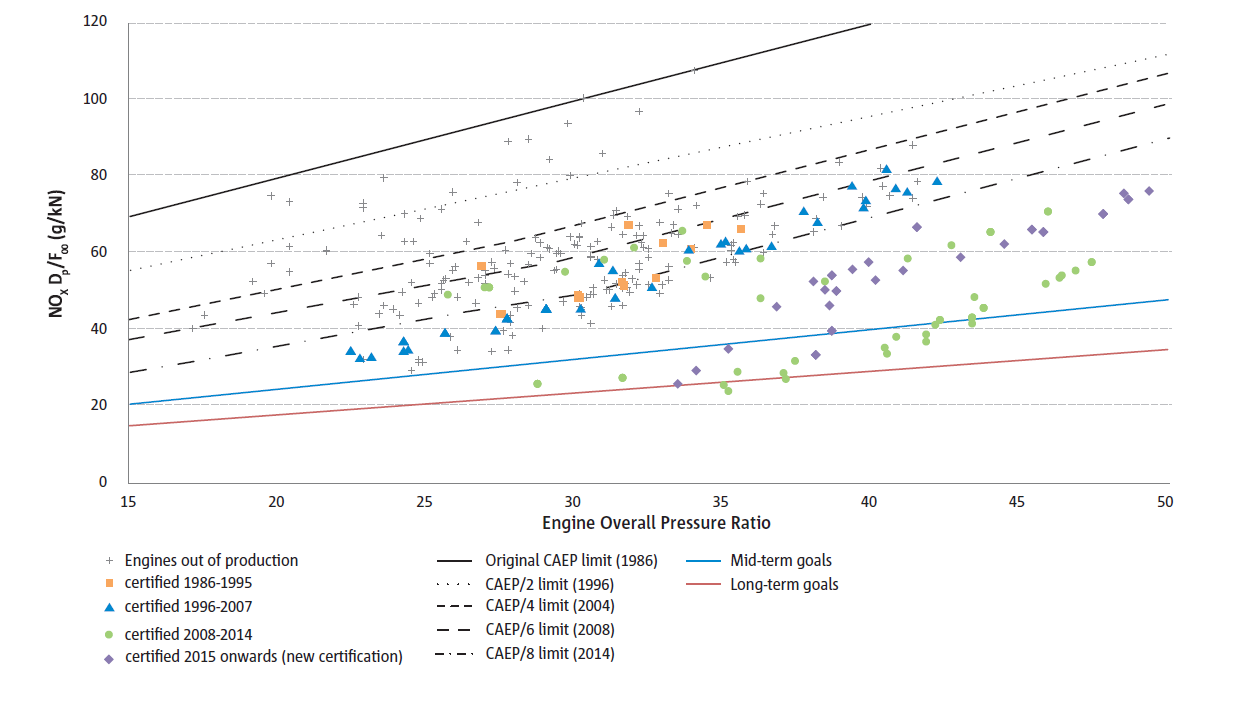
\includegraphics[scale=0.6]{./part0_intro/NOx_emissions_with_OPR}
	\caption[Evolution of NO$_x$ emissions with several generations of aircraft engines]{Evolution of NO$_x$ emissions with several generations of aircraft engines. Source: \citepColor[easa_european_2019]}
	\label{fig:NOX_emissions_with_OPR}
\end{figure}

\begin{figure}[h!]
	\centering
	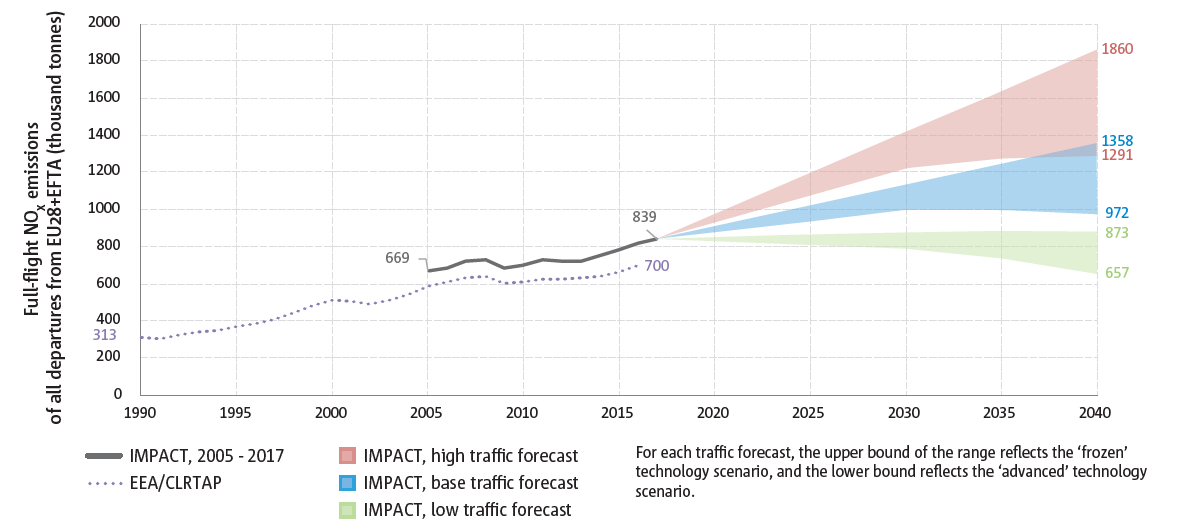
\includegraphics[scale=0.6]{./part0_intro/NOx_emissions_forecast_report2019}
	\caption[NO$_x$ emission forecasts from 2017 to 2040]{NO$_x$ emission forecasts from 2017 to 2040. Source: \citepColor[easa_european_2019]}
	\label{fig:NOX_forecasts}
\end{figure}


\section{Lean combustion in aeronautical gas turbines}

%Conventional combustors used to introduce only a small portion of air ($\sim 30 \%$ ) with the liquid injection system, and the rest was introduced through secondary holes located downstream (see Figure \ref{fig:combustor_conventional}). As a consequence, com

%\begin{figure}[h!]
%	\centering
%	\includegraphics[scale=0.6]{./part0_intro/combustor_conventional}
%	\caption{Conventional combustor. Source: \citeColor[lefebvre_gas_2010].}
%	\label{fig:combustor_conventional}
%\end{figure}

With the objective of reducing NO$_\mathrm{x}$ emissions in aeronautical engines, the community has worked towards the implementation of concepts aiming at producing lean combustion. The motivation for developing lean systems is shown in Figure \ref{fig:NOX_motivation_and_RQL} left: at lean regimes (i.e. with an excess of air), the flame temperature is lower and, consequently, NO$_\mathrm{x}$ formation is reduced. At the same time, emissions of CO, hydrocarbons (HC) and soot are also diminished at this regime (provided that the air excess is not too high, or the emissions will start to grow again). On the other hand, operating at lean regimes will make the system more prone to thermoacoustic instabilities and will place it closer to the the limit of lean blow-out (LBO), hindering ignition and relight capabilities. 

One of the first concepts aiming at reducing emissions is the \textbf{Rich-Burn, Quick-Quench, Lean-Burn} (\textbf{RQL})  \citepColor[novick_low_1981]. RQL systems split the combustion process in three stages. Firstly combustion begins in a fuel-rich primary zone close to the injector, where the NO$_\mathrm{x}$ rate is low (see Figure \ref{fig:NOX_motivation_and_RQL} left). Then, a quick mixing of the unburnt fuel takes place with fresh air to finally burn in lean conditions. This procedure allows to decrease NO$_\mathrm{x}$ emissions as depicted by the low-NO$_\mathrm{x}$ route depicted in Figure \ref{fig:NOX_motivation_and_RQL}. However, a fine and complete fuel atomization is needed so that a fast mixing takes place; otherwise, unburnt fuel could produce extra smoke and soot in the rich-burn region \citepColor[el-asrag_simulation_2007]. This hinders the proper operation of RQL chambers in regimes where fuel can hardly be atomized, such as during altitude relight.

\newpage

\begin{figure}[h!]
	\centering
	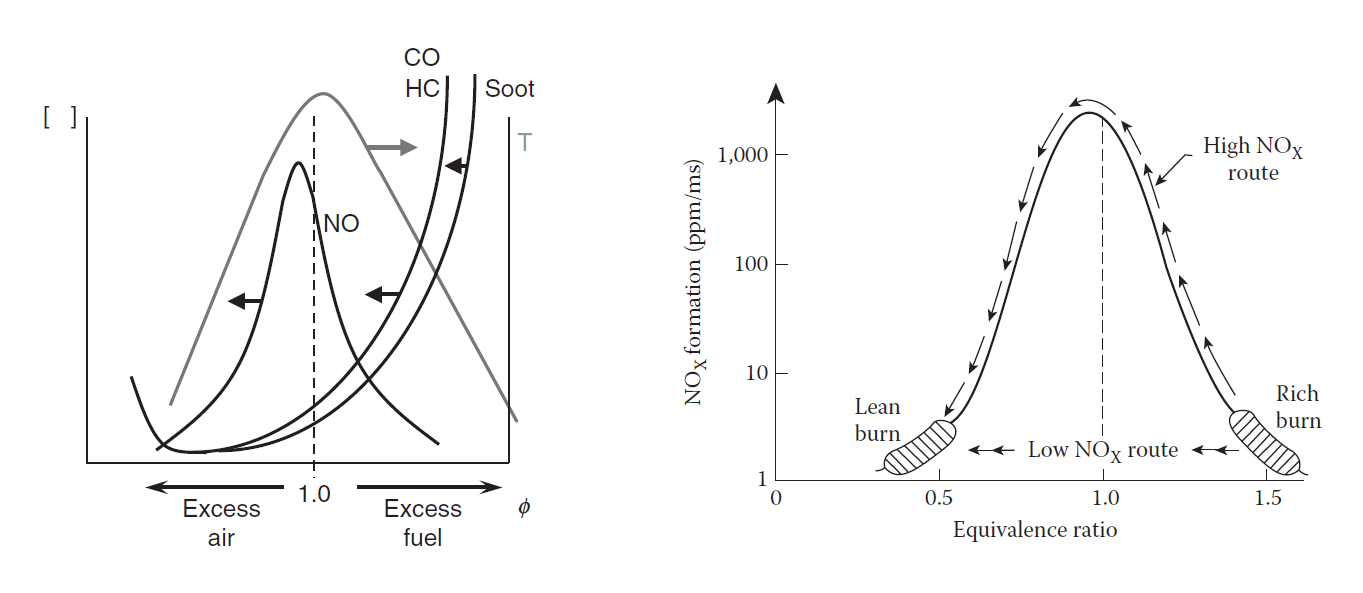
\includegraphics[scale=0.65]{./part0_intro/NOX_motivation_and_RQL}
	\caption{\textsl{Left}: Temperature and species concentration variation with stoichiometric ratio in combustion chambers. Source: \citeColor[dunn-rankin_lean_2008]. \textsl{Right}: NOx formation in Rich-Burn, Quick-Quench, Lean-Burn (RQL) concepts. Source: \citeColor[lefebvre_gas_2010].}
	\label{fig:NOX_motivation_and_RQL}
\end{figure}

The need of reducing NO$_\mathrm{x}$ emissions to the levels settled by authorities led to the development of lean combustion strategies, usually referred as low-NO$_\mathrm{x}$ \citepColor[tacina_low_1990]. In order to foster lean combustion, low-NO$_\mathrm{x}$ concepts introduce an excess of air at the vicinity of the injector: around $70 ~\%$ of air is introduced in the combustion chamber at this location (primary zone), while the rest is used further downstream for effusion cooling. Compared to conventional combustors, where around $30 ~\%$ of air is injected in the primary zone and the rest is introduced further downstream through dilution holes, this allows to reduce the length of the combustion chamber and hence the residence time of combustion, directly linked to NO$_\mathrm{x}$ formation \citepColor[lefebvre_gas_2010]. Furthermore, operating directly at lean regimes will also reduce the formation of soot and CO emissions, which is the main disadvantage of RQL. One of the first lean combustion concepts is the \textbf{Lean Direct Injection} (\textbf{LDI}) technology \citepColor[tacina_low_1990], where fuel is directly introduced into the reaction zone without previous premixing. Lower peak temperatures and residence times are obtained, hence reducing pollutant formation. Contrarily, LDI concepts can produce a non-uniform combustion if mixing is not complete. In this respect, the \textbf{Lean Premixed Prevaporized} (\textbf{LPP}) technology appeared to palliate this issue \citepColor[bittlinger_high_1999]: a premixing length is added before the reaction zone, so that complete evaporation of fuel and mixing can take place before triggering combustion. LPP concepts need, however, a longer combustion chamber to account for the dilution zone, and are more prone to suffer autoignition, flashback and thermoacoustic instabilities.

A good trade-off between both LDI and LPP is obtained with \textbf{Multi-Staged Fuel Injection} (MSFI) \citepColor[pehanhoat_low_2006]. Fuel is introduced in the combustion chamber through two main stages: a \textbf{pilot stage} for flame stabilization purposes, and a \textbf{take-off stage} (also called multipoint ) where the most of premixing takes place (see Figure \ref{fig:foust_TAPS} left). The combination of both injection systems creates a flame that burns in lean conditions and reduces combustion instabilities compared to other low-NO$_\mathrm{x}$ concepts \citepColor[barbosa_time_2009]. The percentage of fuel introduced through each stage can be controlled in order to optimize the combustion performance depending on the flight phase: this procedure is called staging. Considerable reductions in emissions can be obtained with MSFI in conditions where most of NO$_\mathrm{x}$ is produced, such as climb and cruise. Figure \ref{fig:foust_TAPS} right shows the improvements in pollution of a multi-staged fuel injector named Twin Annular Premixing Swirler (TAPS) \citepColor[foust_development_2012] compared to a RQL combustor.

\begin{figure}[h!]
	\centering
	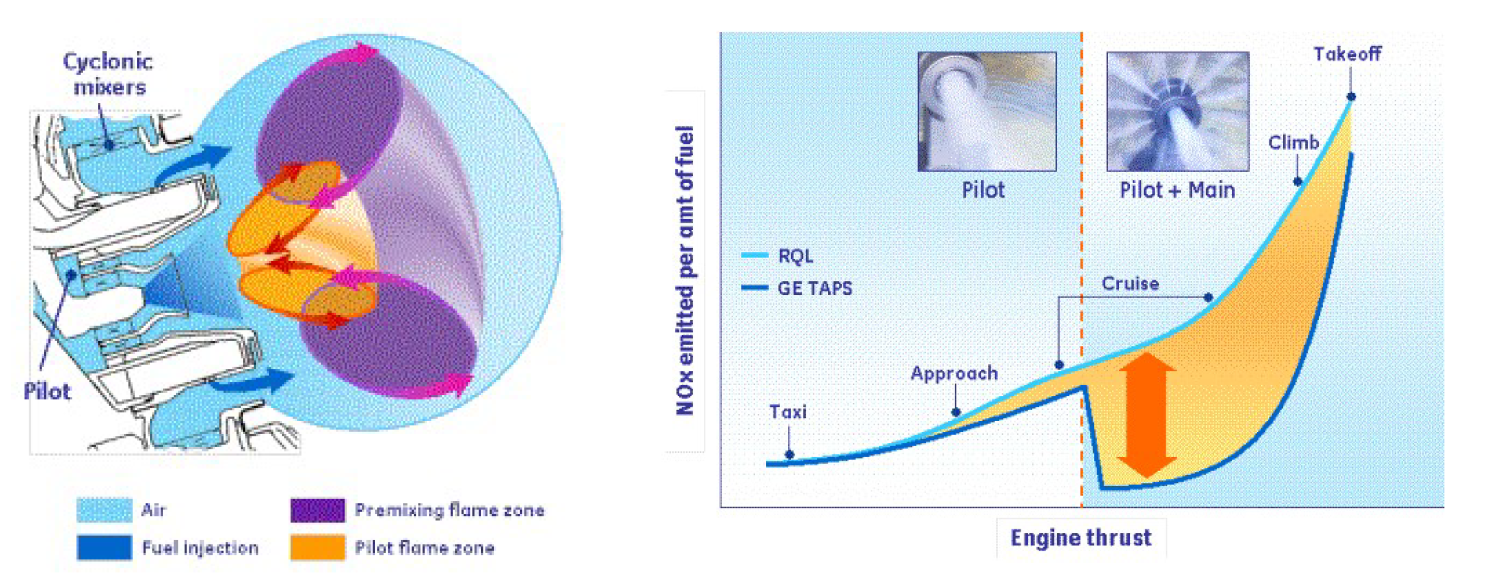
\includegraphics[scale=0.6]{./part0_intro/foust_TAPS}
	\caption{\textsl{Left}: regions in a multi-staged injection system from a TAPS concept. \textsl{Right}: effect of multi-staged injection in NO$_\mathrm{x}$ emissions from a TAPS concept compared to a RQL system. Source: \citeColor[foust_development_2012].}
	\label{fig:foust_TAPS}
\end{figure}

MSFI are a promising technology for fuel injection in aeronautical combustors, and manufacturers such as Safran are working in developing these systems for their application in future engines. Since their main characteristic is fuel staging, processes prior to combustion (such as injection, atomization and mixing) are fundamental for MSFI performance, and their proper comprehension is paramount to optimize such systems. The next sections makes a review on the two-phase flow physical mechanisms of injection and atomization relevant to these injection systems.


\section{Fuel injection technology}
\label{sec:ch1_fuel_injection_technology}

Figure \ref{fig:multipoint_injector_snecma} shows a MSFI injector with the atomization mechanisms present in these systems. Fuel is injected through two inlets: a central nozzle (the pilot stage), where fuel is injected with a pressure-swirl atomizer spreading as a \textbf{hollow cone} spray, and the multipoint injectors located in a crown around the central injector (the take-off stage), where fuel is injected in a \textbf{jet in crossflow} configuration (JICF). As seen in the figure, these two injection systems will produce liquid atomization shortly after the injection location. Furthermore, a third breakup mechanisms is if the opening angle of the hollow cone is large enough; in this case, liquid can impinge the walls of the injector and break due to the interaction between aerodynamics and the liquid wall, forming an \textbf{airblast} spray. As a consequence of these three atomization mechanisms, a dispersed spray will be formed further downstream the injection chamber. This dispersed spray will be later able to evaporate, mix with the surrounding air and burn in the combustion process.

%\begin{figure}[ht]
%     \centering
%     \begin{subfigure}[b]{0.45\textwidth}
%         \centering
%         \includeinkscape[inkscapelatex=false,scale=0.35]{./part0_intro/multipoint_injector_snecma}
%     \end{subfigure}
%     %\hfill
%     \begin{subfigure}[b]{0.45\textwidth}
%         \centering
%          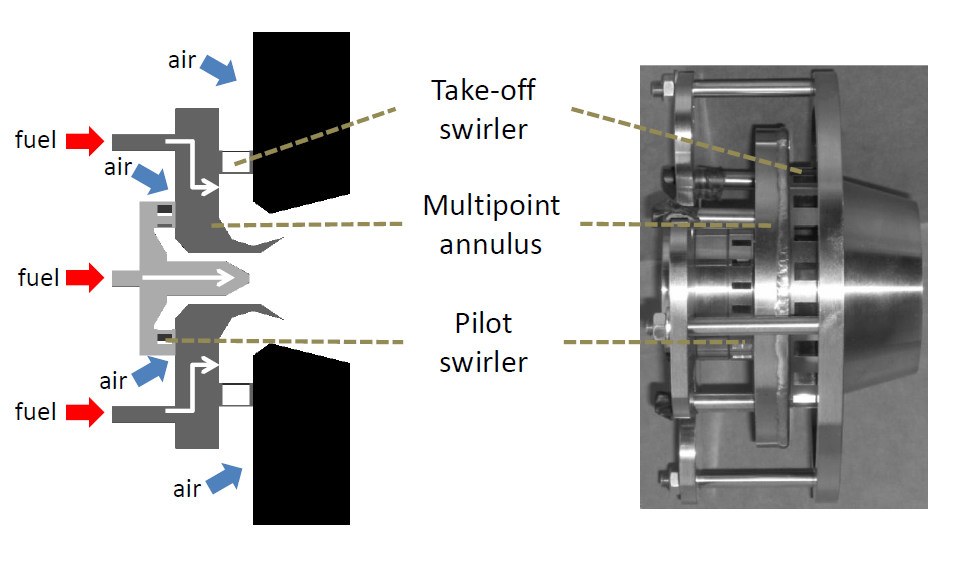
\includegraphics[scale=0.5]{./part0_intro/BIMER_swirler}
%     \end{subfigure}
%        \caption{\textsl{Left}: Size histogram evolution with accumulation time of droplets. \textsl{Right}: comparison of two droplet size histograms from two consecutive time instants.}
%	% See: https://stackoverflow.com/questions/35210337/can-i-plot-several-histograms-in-3d/35225919
%        \label{fig:multipoint_injectors}
%\end{figure}



\begin{figure}[ht]
     \centering
     \includeinkscape[inkscapelatex=false,scale=0.55]{./part0_intro/multipoint_injector_snecma}
      \caption{Multipoint injector from SNECMA (source: \citeColor[jaegle_large_2009]) showing the atomization mechanisms present in MSFI systems.}
      \label{fig:multipoint_injector_snecma}
\end{figure}

A view of the several multiphysical phenomena found within a combustor is shown in Figure \ref{fig:JICF_multiphysics} with an example of reactive liquid jet in crossflow (JICF). Liquid fuel is injected through the injection nozzle as a coherent jet. Instabilities start taking place after injection which will eventually break the jet into large blobs and ligaments during a process known as \textbf{primary atomization} (or primary breakup). Resulting liquid structures will then break into smaller droplets during \textbf{secondary atomization} (or secondary breakup) until the droplets reach a small size and a spherical shape. As a consequence of the atomization process, the specific surface of the spray (i.e. the amount of liquid surface which is in contact with the continuous gas) is large and hence \textbf{evaporation} can take place. Gaseous fuel can then \textbf{mix} with the surrounding air  to produce an ignitable mixture that can finally burn in the \textbf{combustion} process. At the same time, there are other physical mechanisms taking place in the combustion, such as drop-drop interactions, wall-drop interactions and droplet combustion. All these processes are generally found within gas turbines.

\begin{figure}[ht]
     \centering
     \includeinkscape[scale=0.75]{./part0_intro/JICF_multiphysics}
      \caption{Multi-physics phenomena in a reactive jet in crossflow. }
      \label{fig:JICF_multiphysics}
\end{figure}

As illustrated in Figures \ref{fig:multipoint_injector_snecma} and \ref{fig:JICF_multiphysics}, the atomization process is responsible for the generation of droplets. It is necessary that the size of these droplets is small enough so that the liquid specific surface is large and fuel can burn efficiently. Otherwise, unburnt fuel and inefficient combustion can increase the production of pollutants such as NO$_x$ and soot. Understanding the driving mechanisms of atomization is therefore essential for the correct design of atomizers and injectors. However, its study is not trivial due to its multi-scale nature, since it involves a wide range of length-scales from the injector size till the diameter of the smallest droplets, which is often several orders of magnitude smaller.  The rest of this section is then devoted to introducing the fundamentals of atomization and the jet in crossflow phenomenon, which is of special interest for MSFI systems and constitutes a big part of this thesis.

\subsection*{The atomization process}

After liquid injection, atomization is the mechanisms through which coherent, dense liquid is fractured into smaller liquid structures. \citeColor[lefebvre_atomization_2017] define atomization as \textsl{the process by which a liquid jet or sheet is disintegrated by the kinetic energy of the liquid, by the exposure to
high-velocity air or gas, or by mechanical energy applied externally through a rotating or vibrating device}. Its purpose is to increase the liquid specific surface to allow for the evaporation of fuel.

Atomization is triggered by instabilities which are found naturally in liquids jets. \citeColor[rayleigh_instability_1878] found that jet breakup in smaller drops is produced due to the growth of small disturbances in the liquid. Instabilities are amplified by the aerodynamic interaction with the surrounding air, enhancing the energy transfer between both phases. Turbulence of the jet also amplifies these disturbances: if liquid is injected in a high turbulent state, atomization will occur promptly and breakup will be governed by the aerodynamic forces, while if the jet is injected at low speed the breakup will be governed by surface tension and capillary forces, and the breakup morphology will be different. Regimes of atomization are distinguished according to two main dimensionless numbers, the \textbf{Reynolds number} $Re$ and the \textbf{Weber number} $We$:

\begin{equation}
	Re = \frac{\rho u D}{\mu} ~~~~~~ ;  ~~~~~~ We = \frac{\rho u^2 D}{\sigma}
\end{equation}

where $\rho$ is density, $\mu$ the viscosity, $\sigma$ the surface tension, $u$ is a characteristic velocity (usually the liquid velocity or the relative velocities between liquid and gas), $D$ a characteristic length (usually the nozzle diameter or the droplet size). The Reynolds number represents the ratio between the aerodynamic forces and the viscous ones: a high $Re$ indicates a high turbulent state and a dominance of inertia as the main breakup mechanism, while a low $Re$ means laminar flow and a predominant role of viscosity. The Weber number defines the relative importance of aerodynamic forces with respect to capillary forces. From these definitions applied to the liquid phase, $Re_l$ and $We_l$, a third ratio measuring the relative importance between viscous and surface tension forces, called \textbf{Ohnesorge number}, can be defined:

\begin{equation}
Oh = \frac{\sqrt{We_l}}{Re_l} = \frac{\mu_l}{\sqrt{\rho_l D \sigma}}
\end{equation}

\begin{figure}[h!]
	\centering
	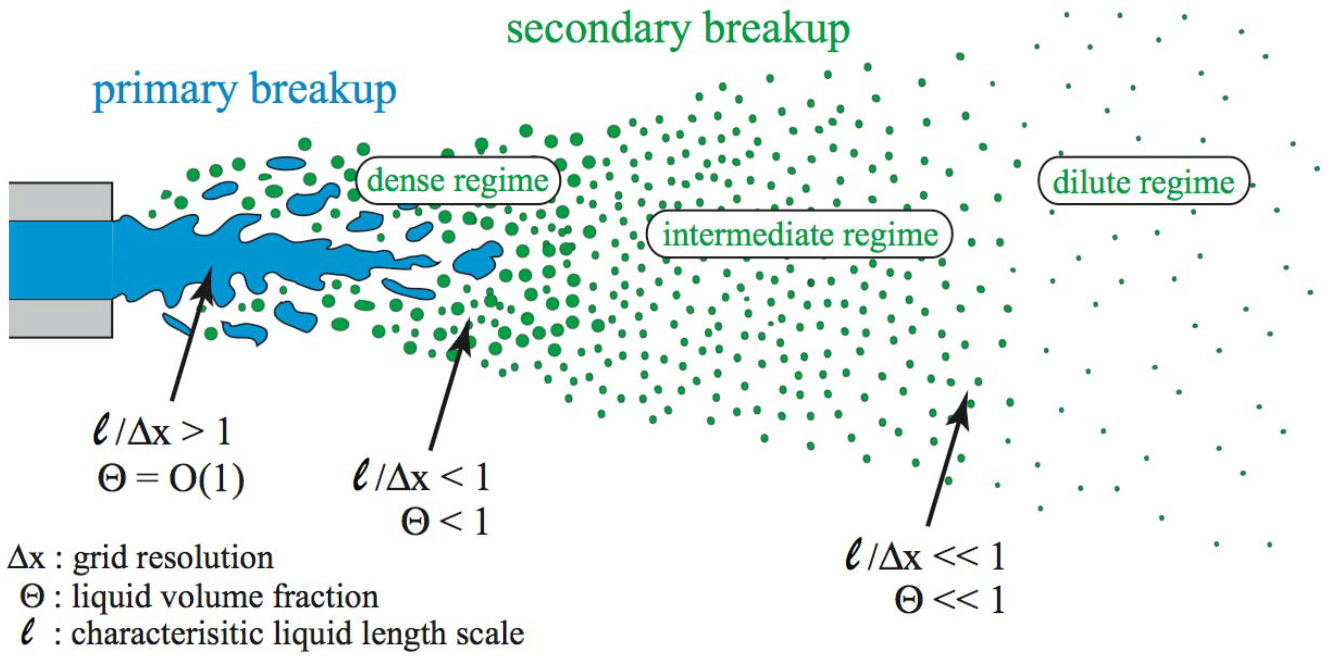
\includegraphics[scale=0.5]{./part0_intro/atomization-regimes-scheme}
	\caption{Atomization breakup regimes. Source: \citeColor[herrmann_modeling_2003]}
	\label{fig:atomization_regimes_herrmann}
\end{figure}

Figure \ref{fig:atomization_regimes_herrmann} illustrates liquid jet injection and atomization. The latter is generally divided by the scientific community in two different regimes, which are commonly found in all disintegrations of jets independently of the injection methodology:

\begin{itemize}

	\item \textbf{Primary atomization} is the process by which a liquid jet or sheet breaks from a dense structure into primary structures such as large blobs and ligaments. It is highly dependent on the injector system (pressure-swirl atomizer, jet in crossflow, airblast ...) and its characteristics (internal geometry, discharge pressure, discharge coefficient, liquid turbulent state ...). As shown in Figure \ref{fig:atomization_regimes_herrmann}, regions where primary atomization takes place are characterized by high characteristic length scales $l$ (larger than the grid resolution) and high liquid volume fractions, features of what is known as the \textbf{dense regime}. Numerical methods targeted to solve for primary atomization are addressed in Chapter \ref{ch3:disperse_phase_methods}. 
	
	Several regimes of primary atomization are distinguished, classified accordingly to the liquid flow state. These regimes, shown in Figure \ref{fig:regimes_atomization_primary}, depend on $Re_l$ and $Oh$ based on the liquid velocity and in the injection diameter $d_0$. As it can be seen, for a fixed value of $Oh$ the governing breakup mechanisms changes if the injection velocity increases (i.e. if $Re_l$ is increases, so turbulence will play a more dominant role). For the $\textbf{Rayleigh regime}$ at low values of $Re_l$, surface tension is the responsible for creating axisymmetric oscillations of the jet with large wavelengths that will make it break into structures larger than the nozzle diameter. Aerodynamic effects are negligible, being capillary forces the leading physical phenomena, and breakup occurs at several nozzle diameter locations downstream the injection point. As $Re_l$ increases, the relative velocity between the liquid and gas phases is higher and aerodynamic forces cannot be neglected, contributing to the destabilizing waves that create droplets of the size of the nozzle diameter and a faster atomization, yet still occurring at several diameters downstream the injector (\textbf{first wind induced} regime). An slightly larger $Re_l$ will swift the dominant breakup role of capillary forces to inertial ones, the wavelenghts of instabilities being amplified by liquid turbulent eddies which break the jet into droplets smaller than the injection nozzle (\textbf{second wind induced}). Finally, at even larger values of $Re_l$ capillary forces can be neglected and the breakup is solely governed by aerodynamics, creating small droplets generated right at the nozzle exit (\textbf{atomization} regime).

	\begin{figure}[h!]
		\centering
		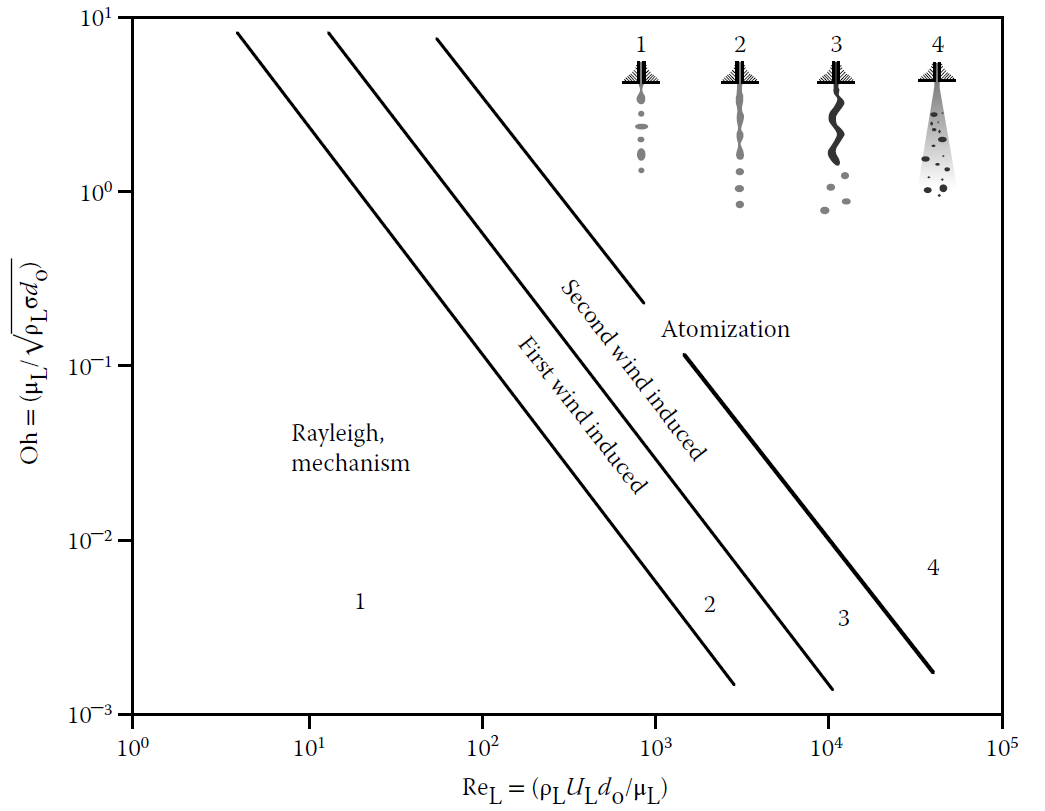
\includegraphics[scale=0.45]{./part0_intro/regimes_atomization_primary}
		\caption{Primary atomization regimes in jets. Source: \citeColor[lefebvre_atomization_2017]}
		\label{fig:regimes_atomization_primary}
	\end{figure}

	
	\item \textbf{Secondary atomization} occurs after primary atomization, once the main liquid structures have been ejected from the jet or sheet and are broken into smaller structures. Injector characteristics and the turbulent state of the coherent liquid do not play a fundamental role anymore, but it is the interaction between the liquid structures and the surrounding air what will dominate secondary breakup. Figure \ref{fig:atomization_regimes_herrmann} shows as secondary atomization disintegrated the liquid structures until a developed spray composed of spherical droplets that do not breakup anymore is formed. During secondary atomization, the spray undergoes a transition from the dense regime found in primary atomization to a \textbf{dilute regime} where the characteristic length scales of liquid (i.e. the droplets diameters) are very small and the liquid volume fraction is very low. Between the dense and dilute regimes, an \textbf{intermediate} regime can be defined where values of volume fraction and comprised between those of the dense and dilute ones. The lower liquid volume fractions and small sizes (usually smaller than the mesh resolution) found in these regimes require numerical resolution through methods different from those devoted to resolve primary atomization. Such methods are introduced in Chapter \ref{ch3:disperse_phase_methods}.
	
	As the main phenomenon governing secondary atomization is the interaction between the liquid and the gas, this process can be characterized by means of the Weber number based on the relative velocity between phases:
	
	\begin{equation}
	We = \frac{\rho_g u_\mathrm{rel}^2 r}{\sigma} 
	\end{equation}
	
	where $u_\mathrm{rel} = | u_l - u_g  |$ and $r$ is a characteristic length of the liquid structures (the radius for spherical droplets). The gaseous density is taken as representative one. Different regimes of primary atomization, universal for any injector geometry and injection system, are depicted in Figure \ref{fig:regimes_atomization_secondary}. For large numbers of $We$ (i.e. high relative velocities and/or large length scales) the breakup is \textbf{catastrophic}, and particles are disintegrated into a large number of very small droplets due to shear forces causing stripping. As $We$ decreases the topology of structures found during atomization changes and breakup becomes less aggressive. For small values of $We$, particles split into a small number of droplets due to \textbf{bag} or \textbf{vibrational} breakups. For $We < 12$, breakup hardly occurs and droplets are said to be in equilibrium with the surrounding air: atomization is complete. This value is called the \textbf{critical Weber number}. 
	
	The interactions among droplets (drop-drop) and between droplets and walls (drop-wall), both illustrated in Figure \ref{fig:JICF_multiphysics} also produce secondary atomization with different governing mechanisms than the drop-air interaction. These particular phenomena are not addressed in this thesis and hence they will not be further discussed.
	
	\begin{figure}[h!]
		\centering
		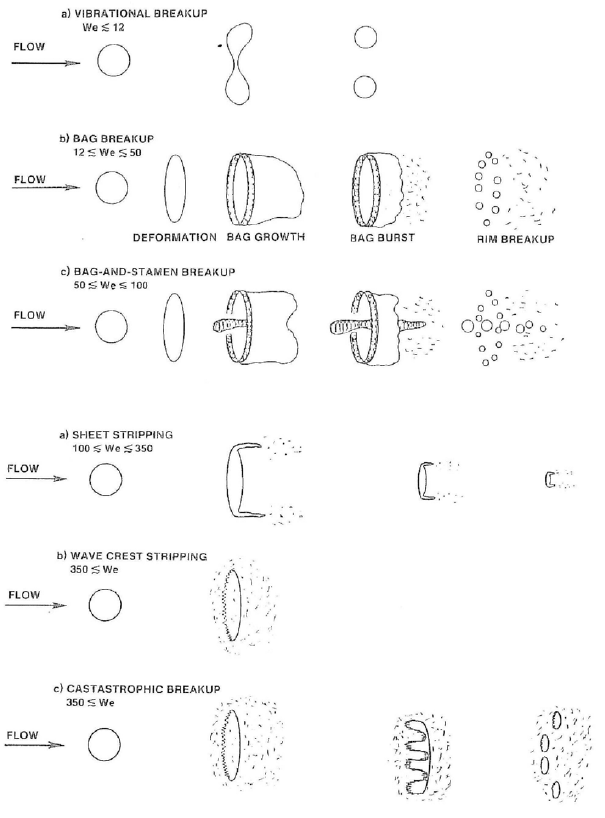
\includegraphics[scale=1.0]{./part0_intro/regimes_atomization_secondary}
		\caption{Secondary atomization regimes. Source: \citeColor[pilch_use_1987]}
		\label{fig:regimes_atomization_secondary}
	\end{figure}

\end{itemize}



\subsection*{Liquid jet in crossflow}

Contrarily to secondary atomization, whose behaviour is not influenced by the injection system, primary atomization is highly dependent on the injector configuration. As a consequence, different liquid structures and characteristic sizes are present in MSFI systems due to the different atomization mechanisms (see Figure \ref{fig:multipoint_injector_snecma}). One characteristic breakup mechanism of MSFI is the one from the take-off stage, which injects fuel in a particular configuration known as liquid jet in crossflow (JICF). This section discusses primary atomization and the influencing parameters of JICF, which is the injection configuration studied in this thesis.

In a liquid JICF, a stream of air flows perpendicularly to the direction of liquid injection, as shown in Figure \ref{fig:JICF_multiphysics}. The liquid jet leaves the nozzle and bends towards the crossflow direction, undergoing primary and secondary atomization which creates a developed spray further downstream the injection point. The aerodynamic interaction with the surrounding air is of paramount importance: it influences the jet breakup, vertical penetration and the atomization process, which will eventually affect the mixing process prior to combustion in reactive applications.

%\subsubsection*{Breakup process}

The atomization process in liquid JICF has been investigated experimentally by several authors \citemColor[adelberg_breakup_1968,wu_breakup_1997,becker_breakup_2002,ragucci_trajectory_2007,freitag_spray_2008]. These studies have generally identified two main mechanisms of primary breakup:

\begin{itemize}

	\item \textbf{Column breakup}. Surface waves on the liquid column start to grow until the jet breaks into ligaments, which eventually turn into droplets during secondary atomization. An example is shown in Figure \ref{fig:JICF_breakup_mechanisms_freitag} left, showing the surface waves caused by instabilities. This type of breakup occurs when the aerodynamic interaction is not too strong (low relative liquid-air velocities).

\item \textbf{Surface breakup}. A strong aerodynamic interaction (large relative liquid-air velocity, high viscosity, etc.) produces the disintegration of the liquid jet by means of shear. Ligaments and droplets are
stripped off the sides of the jet, which eventually is torn apart into droplets. Surface breakup can be appreciated in Figure \ref{fig:JICF_breakup_mechanisms_freitag} right. 

\end{itemize}

\begin{figure}[h!]
	\centering
	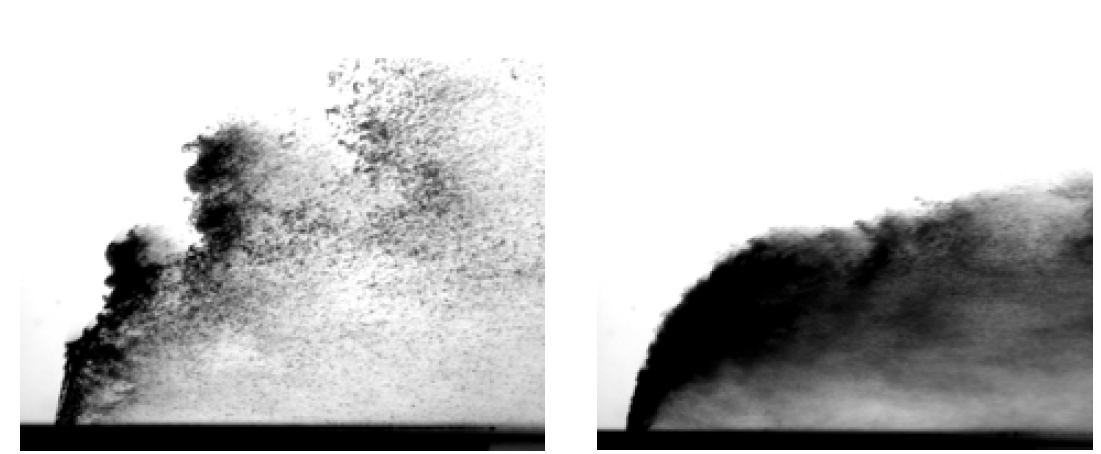
\includegraphics[scale=0.65]{./part0_intro/JICF_breakup-mechanisms_freitag}
	\caption{Experimental images of kerosene JICF breakup. \textsl{Left}: column breakup. \textsl{Left}: surface breakup. Source: \citeColor[freitag_spray_2008]}
	\label{fig:JICF_breakup_mechanisms_freitag}
\end{figure}

As in any two-phase problem, the physical and breakup characteristics of a JICF can be represented by means of dimensionless numbers. In liquids jet in crossflow, the main two governing factors are the \textbf{momentum flux ratio} $q$ and the \textbf{Weber number based on the gaseouos phase} $We_g$, defined in Eq. (\ref{eq:q_and_We_JICF_parameters}). The former parameter represents the relation between the momentum, or kinetic energies, of the liquid and gaseous phases, while the latter represents the relative contribution of the gaseous phase to capillary forces. 

\begin{equation}
\label{eq:q_and_We_JICF_parameters}
	q = \frac{\rho_l u_l^2}{\rho_g u_g^2} ~~~~~~ ;  ~~~~~~ We_g = \frac{\rho_g u_g^2 d_\mathrm{inj}}{\sigma}
\end{equation}

The influence of these factors in the breakup process of liquid jets in crossflow has been experimentally studied by \ref{fig:jicf_breakup_regime_wu}, resulting in a breakup map of Figure \ref{fig:jicf_breakup_regime_wu}. Column and surface breakup, which are the main primary atomization regimes, are separated by the dividing line that indicates the transitional $q$ value between both regimes to be inversely proportional to $We_g$. For column breakup, several atomization modes appear depending on the value of $We_g$. Figure \ref{fig:jicf_breakup_sallam} shows experimental snapshots of these modes. As it is shown, for low $We_g$ (capillary and bag regimes) the breakup is dominated by capillary forces and the jet stays coherent until several nozzle diameters downstream the injection point, once the jet has bent and its cross section has been deformed. Waves are clearly observed in the windward side of the jet (i.e. the face in contact with the incoming air), and the wavelength of liquid surfaces $\lambda$ can be defined as the distance between two nodes.  For higher $We_g$ (multimode and shear regimes), instabilities causing breakup are also observed developing along the windward side of the jet, but it is also noticeable the stripping of liquid ligaments and droplets at the sides of the jets due to aerodynamic shear. For the shear breakup these stripped-off structures appear close to the injection point, hindering the optical access to the jet structure and atomization characteristics further downstream. This was also observed for the surface breakup mode in Figure \ref{fig:JICF_breakup_mechanisms_freitag} right. Another noticeable characteristic is that the wavelengths $\lambda$ decrease for larger values of $We_g$. \citeColor[sallam_breakup_2004] found that the order of magnitudes of the wavelenghts with respect to the injection diameter is $\lambda/d_\mathrm{inj} > 1$ for capillary breakup, $\lambda/d_\mathrm{inj} \approx 1$ for bag breakup, $0.1 < \lambda/d_\mathrm{inj} < 1$ for the multimode regime and $\lambda/d_\mathrm{inj} \approx 0.1$ for shear breakup. The main responsible mechanisms of generating these surface waves are either Kelvin-Helmholtz and Rayleigh-Taylor instabilities. The former ones are said to be the dominating mechanisms for the waves observed in Figure \ref{fig:jicf_breakup_sallam} \citepColor[sallam_breakup_2004]. It is believed that the prevalence of either one or another mode depends on the density ratio between fluid and gas, being the Rayleigh-Taylor the main dominant mechanisms for high density rations \citepColor[ghods_detailed_2013]. Nevertheless, the appearance and dependence of each instability mode is not certainly known nowadays and remains an open question requiring further research.

\begin{figure}[h!]
	\centering
	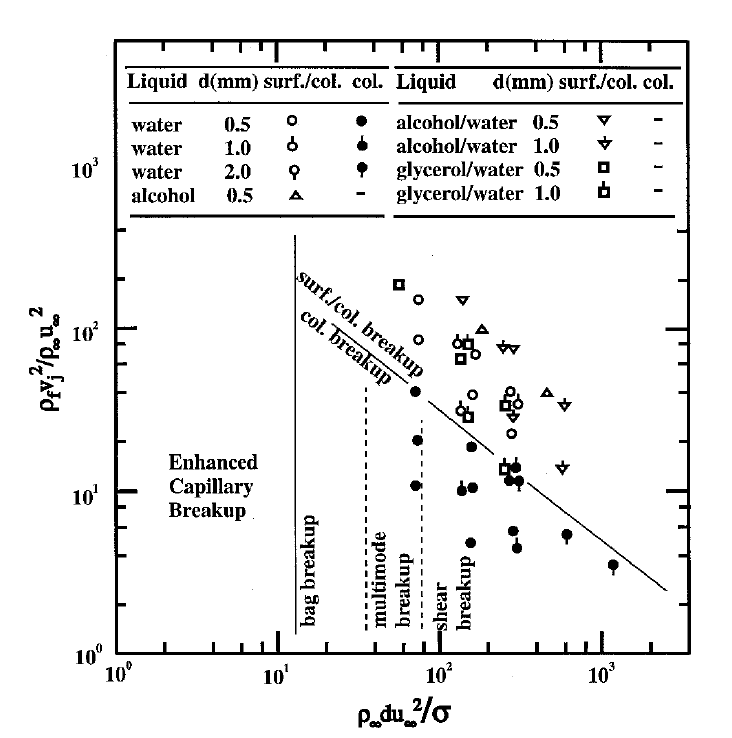
\includegraphics[scale=0.55]{./part0_intro/jicf_breakup_regime_wu}
	\caption{Breakup map for liquid jet in crossflow. Source: \citeColor[wu_breakup_1997]}
	\label{fig:jicf_breakup_regime_wu}
\end{figure}

\begin{figure}[h!]
	\centering
	\includeinkscape[inkscapelatex=true,scale=0.7]{./part0_intro/jicf_breakup_sallam}
	\caption[Primary breakup processes in liquid jet in crossflow]{Primary breakup processes in liquid jet in crossflow. Air flows from right to left. (a) No breakup, $We_g = 0$. (b) Capillary breakup, $We_g = 3$. (c) Bag breakup, $We_g = 8$. (d) Multimode breakup, $We_g = 30$. (e) Shear breakup, $We_g = 220$. Source: \citeColor[sallam_breakup_2004]}
	\label{fig:jicf_breakup_sallam}
\end{figure}

Another very important characteristic of the liquid jet in crossflow is its penetration, since in real configurations it will determine the region where evaporation and mixing takes place and, later, the flame structure. The near-field jet penetration can be quantified by means of the \textbf{vertical trajectory} of the jet, which gives the mean contour of its windward side. This trajectory can be experimentally obtained either from instantaneous snapshots of the jet (Figure \ref{fig:inst_and_mean_jets_ragucci} left) or from average images (Figure \ref{fig:inst_and_mean_jets_ragucci} right), each experimentalist using its own methods. From experimental studies, the trajectory is generally given by correlations relating the vertical trajectory $z$ with the axial coordinate $x$. Some experimental correlations are shown in Table \ref{tab:correlations_experimental_JICF}, where $We_{ae} = \rho_g u_l^2 d_\mathrm{inj}/\sigma$. Figure \ref{fig:inst_and_mean_jets_ragucci} right shows the jet correlation from \citeColor[ragucci_breakup_2007] overlapped with the average jet view.


\begin{figure}[h!]
	\centering
	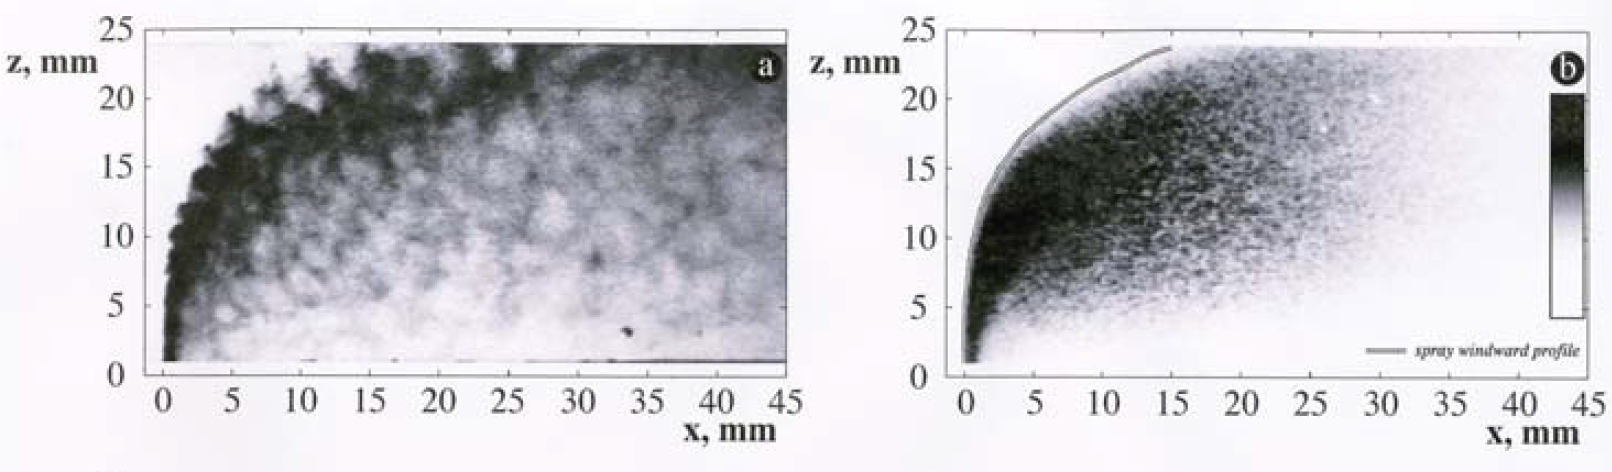
\includegraphics[scale=0.6]{./part0_intro/ragucci_jet_penetration}
	\caption{Instantaneous and averages images of a liquid jet in crossflow. Source: \citeColor[ragucci_breakup_2007]}
	\label{fig:inst_and_mean_jets_ragucci}
\end{figure}


\begin{table}[!h]
\centering
\caption{Correlations for the jet trajectory of the JICF}
\begin{tabular}{c|c|c|c}
\hline
$z / d_\mathrm{inj}$ & Liquid  & Range of validity & Reference  \\
\hline
\hline
\multirow{2}{*}{$1.37 \sqrt{q \left( \frac{x}{d_\mathrm{inj}} \right)}$} & \multirow{2}{*}{ Water } & $3.4 < q < 185$ & \multirow{2}{*}{\citeColor[wu_breakup_1997]} \\
& & $57 < We_{ae} < 1200$ & \\
\hline
\multirow{3}{*}{$1.57 \mathrm{q}^{0.36} \ln \left( 1 + 3.81 \frac{x}{d_\mathrm{inj}} \right)$} & \multirow{3}{*}{ Kerosene } & $1 < q < 12$  & \multirow{3}{*}{\citeColor[becker_breakup_2002]} \\
& & $90 < We_{ae} < 2120$ &  \\
& & $2 < x/d_\mathrm{inj}< 22$ & \\
\hline
\multirow{2}{*}{ $2.27 q^{0.44} We_{ae}^{-0.012} \left( \frac{x}{d_\mathrm{inj}} \right)^{0.367}$ }  & \multirow{2}{*}{Kerosene} & $5 < q < 280$  & \multirow{2}{*}{\citeColor[ragucci_breakup_2007]} \\
& & $7 < We_{ae} < 340$ & \\
\hline
\multirow{3}{*}{ $1.6 q^{0.4} \ln \left( 1 + 3.81 \left( \frac{x}{d_\mathrm{inj}} \right) \right)$} & \multirow{3}{*}{Kerosene} & $3 < q < 24$ & \multirow{3}{*}{\citeColor[freitag_spray_2008]} \\
& & $39 < We_{ae} < 3281$ & \\
& & $1.4 < x/d_\mathrm{inj}< 50$ & \\
\hline
\end{tabular}
\label{tab:correlations_experimental_JICF}
\end{table}


%\begin{table}[!h]
%\centering
%\caption{Correlations for the jet trajectory of the JICF}
%\begin{tabular}{c|c|c|c}
%\hline
%$z / d_\mathrm{inj}$ & Liquid  & Range of validity & Reference  \\
%\hline
%\hline
%$1.37 \sqrt{q \left( \frac{x}{d_\mathrm{inj}} \right)}$ & Water & $3.4 < q < 185$ &\citeColor[wu_breakup_1997] \\
%\hline
%$2.27 q^{0.44} We_{ae}^{-0.012} \left( \frac{x}{d_\mathrm{inj}} \right)^{0.367}$   & Kerosene & $5 < q < 280$  & \citeColor[ragucci_breakup_2007] \\
%\hline
%\multirow{2}{*}{ $1.6 q^{0.4} \ln \left( 1 + 3.81 \left( \frac{x}{d_\mathrm{inj}} \right) \right)$} & \multirow{2}{*}{Kerosene} & $3 < q < 24$ & \multirow{2}{*}{\citeColor[freitag_spray_2008]} \\
%& & $1.4 < x/d_\mathrm{inj}< 50$ & \\
%\hline
%\end{tabular}
%\label{tab:correlations_experimental_JICF}
%\end{table}


In general, all the correlations from Table \ref{tab:correlations_experimental_JICF} show a dependence of the jet trajectory with the injection diameter $d_\mathrm{inj}$ and the momentum flux ratio $q$. These are the two main parameters governing the jet penetration. The larger the injection diameter, the further the jet will penetrate. This is attributed to a more coherent jet: if $d_\mathrm{inj}$ increases, more liquid mass flow is injected, so the jet carries more momentum and is able to withstand more stiffly the
interaction with the airstream. Furthermore, atomization of a thicker jet will produce larger droplets that
will travel further due to their ballistic properties. For the momentum flux ratio, increasing its value also increases the jet penetration. This is clearly seen in Table \ref{tab:correlations_experimental_JICF}, as the exponent factor of $q$ is positive in all correlations. Figure \ref{fig:parametric_JICF_q_ratio} shows the $q$ effect in the jet penetration. Regarding the influence of the air velocity (or equivalently, $We_g$), it does not have a direct effect in the jet penetration, as the correlations from Table \ref{tab:correlations_experimental_JICF} do not show any dependence with $We_g$. This is observed in Figure \ref{fig:parametric_JICF_air_velocity}, which shows instantaneous snapshots of a liquid JICF for several values of $u_g$. The main effect of increasing the gas velocity is the transition from column to surface breakup mechanisms, as given by the breakup map of Figure \ref{fig:jicf_breakup_regime_wu}. Nevertheless, it is seen that by increasing $u_g$, the far-field penetration is reduced due to a finer atomization: for low values of $u_g$, column breakup generates bigger droplets whose ballistic properties allow them to penetrate further in the vertical direction, while higher values of the gas velocity generate smaller droplets both from surface and column breakup mechanisms that will relax faster towards the air velocity and direction. \citeColor[becker_breakup_2002] tested a kerosene JICF with several gas velocities and measured the granulometry of the developed spray at a plane located 80 mm downstream the injection nozzle, obtaining the following relation between the Sauter Mean Diameter (SMD) and the kinetic energy of the gas which confirms how the mean droplet size decreases with increasing gas velocity:

\begin{equation}
SMD = 429 \left( \rho_g u_g^2 \right)^{-0.24}
\end{equation}



\begin{figure}[h!]
	\centering
	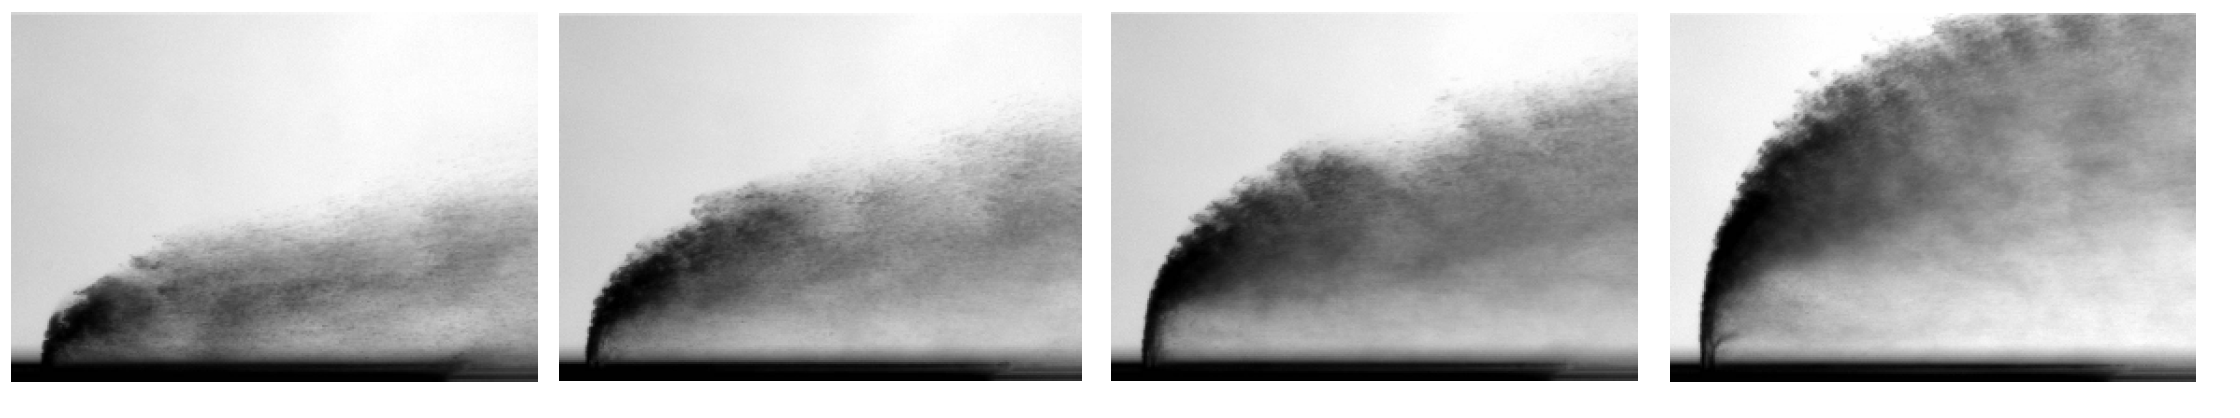
\includegraphics[scale=0.45]{./part0_intro/parametric_JICF_q_ratio}
	\caption{Effect of $q$ ratio. From left to right: $q = 3, 6, 12, 24$. Fixed values: $d_{inj} = 0.5 ~mm$, $u_g = 75 ~m/s$, $p_\infty = 4 ~\mathrm{bar}$. Source: \citeColor[freitag_spray_2008].}
	\label{fig:parametric_JICF_q_ratio}
\end{figure}

\begin{figure}[h!]
	\centering
	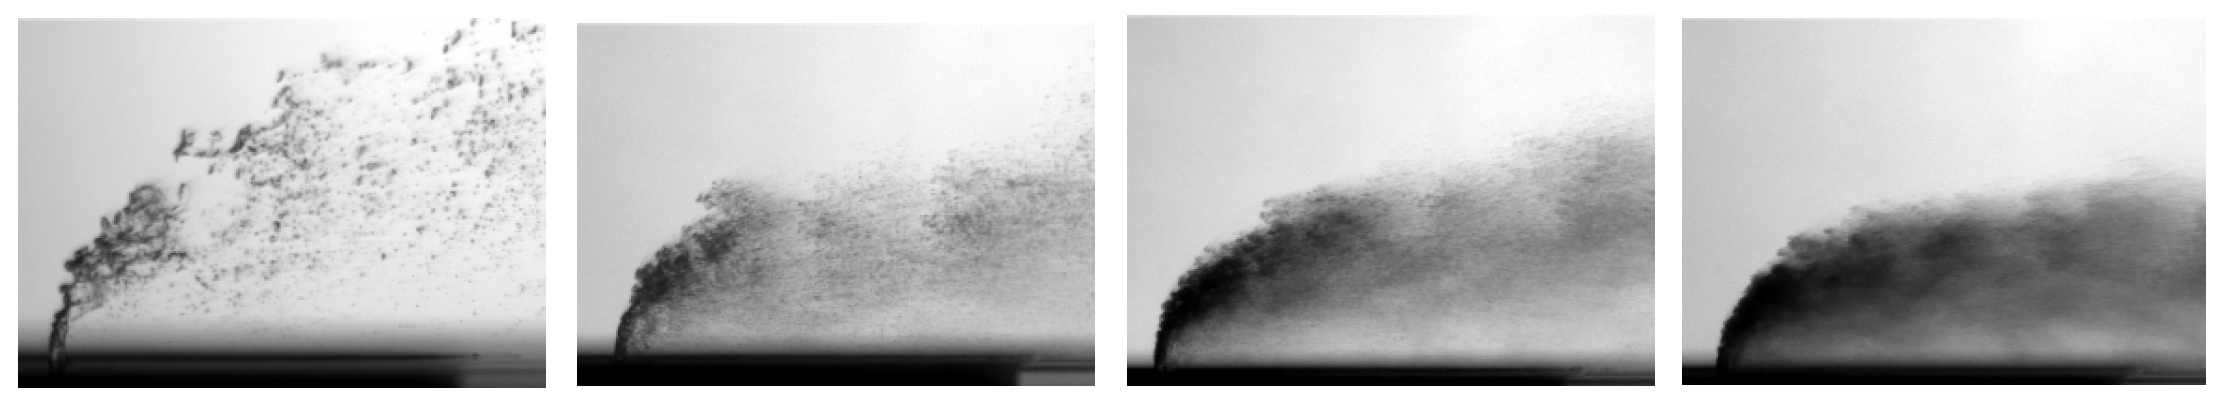
\includegraphics[scale=0.45]{./part0_intro/parametric_JICF_air_velocity}
	\caption{Effect of air velocity. From left to right: $u_g = 25, 50, 75, 100 ~m/s$. Fixed values: $d_{inj} = 0.5 ~mm$, $q = 6$, $p_\infty = 4 ~\mathrm{bar}$. Source: \citeColor[freitag_spray_2008].}
	\label{fig:parametric_JICF_air_velocity}
\end{figure}

%Regarding internal nozzle effects Internal nozzle effects: effect of L/D ratio, some words on cavitation and hydraulic flip (ref. Chemloul).

\section{Numerical simulations of fuel injection and combustion }

The previous section has illustrated the heterogeneity of phenomena which are found in injection systems relevant to gas turbines, with a special focus on MSFI technology aiming at reducing NO$_\mathrm{x}$ formation. The study of these phenomena with experimental facilities is often restricted to academic cases without complex geometries due to difficult optic visualization. Furthermore, experiments do not have access to all the magnitudes of interest involved in the problem, and in some cases involving combustion or detonation they can involve safety issues.

An alternative to study and design injection and combustion systems is the use of numerical simulations with Computational Fluid Dynamics (CFD). This tool has gained popularity in the last decades due to the increase in computational performances and the appearance of High Performance Computing (HPC), which allows to perform simulations of complex problems in parallel machines. CFD simulations can provide insightful information in the physical mechanisms and variables of interest, they do not have limitations regarding optical access and are free of hazards. Therefore, numerical simulations have become a powerful tool for the design of combustion systems and the understanding of the underlying fundamental physical phenomena.

In order to resolve a given physical problem, the proper modeling strategy and numerical methods to perform CFD simulations must be chosen. Depending on the required accuracy and the computational resources available, three main approaches can be used to resolve numerically the Navier-Stokes equations. From lower to higher accuracy (and equivalently, from lower to higher computational cost), these approaches are:

\begin{enumerate}

	\item \textbf{Reynolds Averaged Navier Stokes} (RANS). The governing equations are averaged and the mean flow field is solved. Extra terms appear in the equations which need closure terms. All the turbulence spectrum, from Taylor to Kolmogorov characteristic length scales, is modelled. RANS can provide mean values and are good to characterize pressure drop in certain configurations, but are not best suited for solving transient problems.
	
	\item \textbf{Large-Eddy Simulations} (LES). A low-pass filter is applied to the Navier-Stokes equations, so that the characteristic scales under the filter size are modelled and the scales with larger size are resolved. For solving the smallest scales, a turbulence model is required which accounts for the viscous dissipation. One of the most well-known filters is the Smagorinsky model \citemColor[smagorinsky_general_1963,germano_dynamic_1991].
	
	\item \textbf{Direct Numerical Simulations} (DNS). In such simulations, all the turbulence characteristic scales are solved and no models are applied. Hence, DNS is an accurate tool for properly resolving turbulence. Nevertheless, its high computational cost reduces the application of DNS to reduced geometries and canonical test cases, and nowadays its application to full industrial configurations is not reachable.

\end{enumerate}

These three methodologies are widely used for aerodynamic and hydrodynamic problems involving one fluid phase. Two-phase flow problems also make use of these equations, but they additional equations or modeling tools to consider the interaction between phases. For cases involving liquid and gas, which are of interest in automotive and aeronautical engines, this interaction is dominated by surface tension $\sigma$. In terms of numerical modeling, surface tension creates a discontinuity in pressure and viscosity (as demonstrated later in $\S$\ref{sec:ch2_governing_equations}) that needs to be dealt with mathematical tools, for instance by adding extra forcing terms in the governing equation for momentum. Furthermore, different methods and modeling methodologies will be used depending on the problem to solve, since the multi-scale, complexity and richness of the physical phenomena in two-phase flows (illustrated in $\S$\ref{sec:ch1_fuel_injection_technology}) does not allow to use a single numerical formalism to solve simultaneously all processes involved.

One large family of numerical methods is the one devoted to resolve accurately atomization. The underlying interest is to capture the dynamics of primary and secondary atomization, its governing physical mechanisms and the interaction with the gaseous phase. For this purpose, the main approach is to perform CFD simulations where the Navier-Stokes equations are resolved for each phase with LES or DNS. Then, additional equations are added in order to determine the evolution of the interface (e.g. level-set methods) or the liquid volume fraction (e.g. volume of fluid methods). These simulations are usually denoted as \textbf{resolved} or \textbf{eulerian}. Figure \ref{fig:DNS_simulations_jets} shows two instantaneous jets solved with a resolved atomization approach, where the interface dynamics have been solved with level-set methods. A diesel jet coloured by axial velocity and a liquid jet in crossflow are shown. In both cases, ligaments and droplets generated by the atomization process can be clearly appreciated. In this document, Chapter \ref{ch2:numerical_methods_resolved_atomization} presents numerical methods used nowadays for resolving injection and atomization.

\begin{figure}[h!]
	\centering
   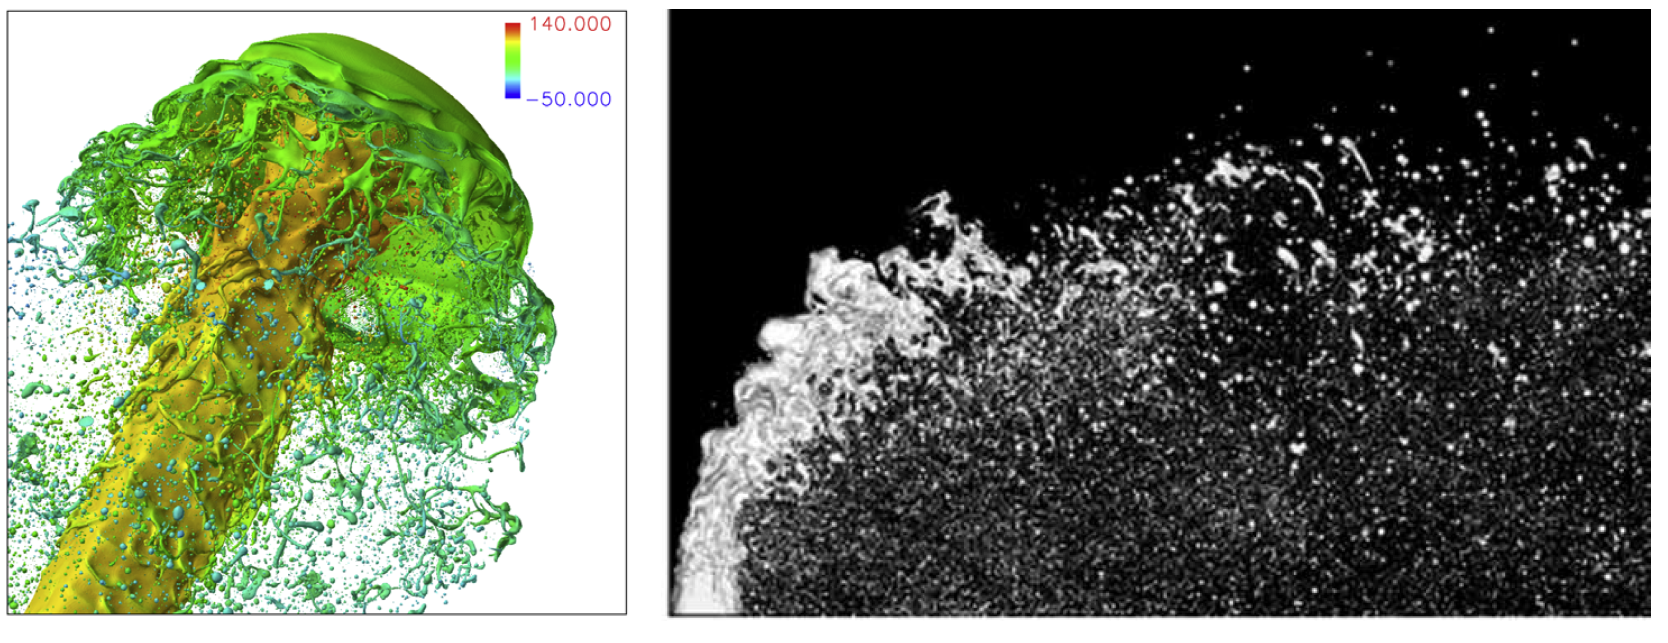
\includegraphics[scale=0.4]{./part0_intro/jets_DNS_simulations}
	\caption[Direct numerical simulations of primary atomization in liquid jets.]{Direct numerical simulations of primary atomization in liquid jets. \textsl{Left}: diesel jet, from \citepColor[shinjo_simulation_2010]. \textsl{Right}: liquid jet in crossflow, from \citeColor[herrmann_detailed_2009].}
	\label{fig:DNS_simulations_jets}
\end{figure}

Methodologies for resolving atomization are envisaged to capture the multi-scale nature of atomization, dedicating huge computational resources to solve from the biggest to the smallest scales and the interaction between phases. Nevertheless, the size of the smallest structures and droplets captured are often limited by the grid resolution, and due to their high cost cannot be easily coupled with additional physical equations to solve for the evaporation and combustion processes. To tackle these problems, different strategies are used, often circumventing atomization by injecting a spray represented by liquid spherical particles. These particles compose a \textbf{dispersed-phase system} where the gaseous phase is resolved by the Navier-Stokes equations and the particles representing the liquid phase evolve according to the dynamics of point-particle systems in \textbf{lagrangian simulations}. The coupling between both phases is done through exchange terms of mass, momentum and energy, and hence evaporation and combustion can be easily modelled in these simulations. Figure \ref{fig:lagrangian_simulations_jets} shows also two jets, diesel and jet in crossflow, simulated with lagrangian approaches. Contrarily to the resolved jets of Figure \ref{fig:DNS_simulations_jets}, here all the liquid phase is represented by means of spherical particles and the dynamics of atomization are not appreciated. In contrast, these simulations are computationally much cheaper than the former ones and can be applied to reactive computations in complex geometries as shown in Figure \ref{fig:lagrangian_simulations_jets}, where a full combustor is studied. In lagrangian simulations, the injection process is fundamental and needs to be properly modeled by injecting the right droplets sizes and velocities distributions. Chapter \ref{ch3:disperse_phase_methods} shows the state of the art on several numerical tools to approach dispersed two-phase phase systems, with special emphasis on lagrangian methods and their application to approach liquid jet in crossflow injection.

\begin{figure}[h!]
	\centering
   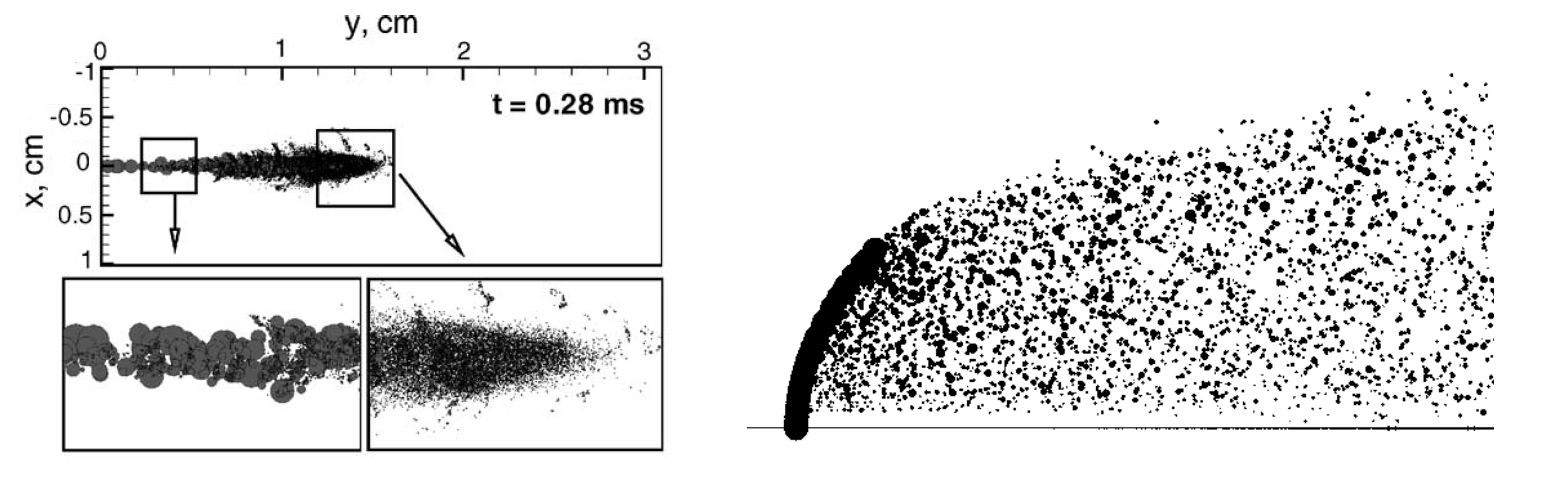
\includegraphics[scale=0.5]{./part0_intro/jets_lagrangian_simulations}
	\caption[Lagrangian simulations of liquid jets.]{Lagrangian simulations of liquid jets. \textsl{Left}: diesel jet, from  \citeColor[apte_les_2003]. \textsl{Right}: liquid jet in crossflow, from \citeColor[behzad_kiva-based_2010].}
	\label{fig:lagrangian_simulations_jets}
\end{figure}

\begin{figure}[h!]
	\centering
   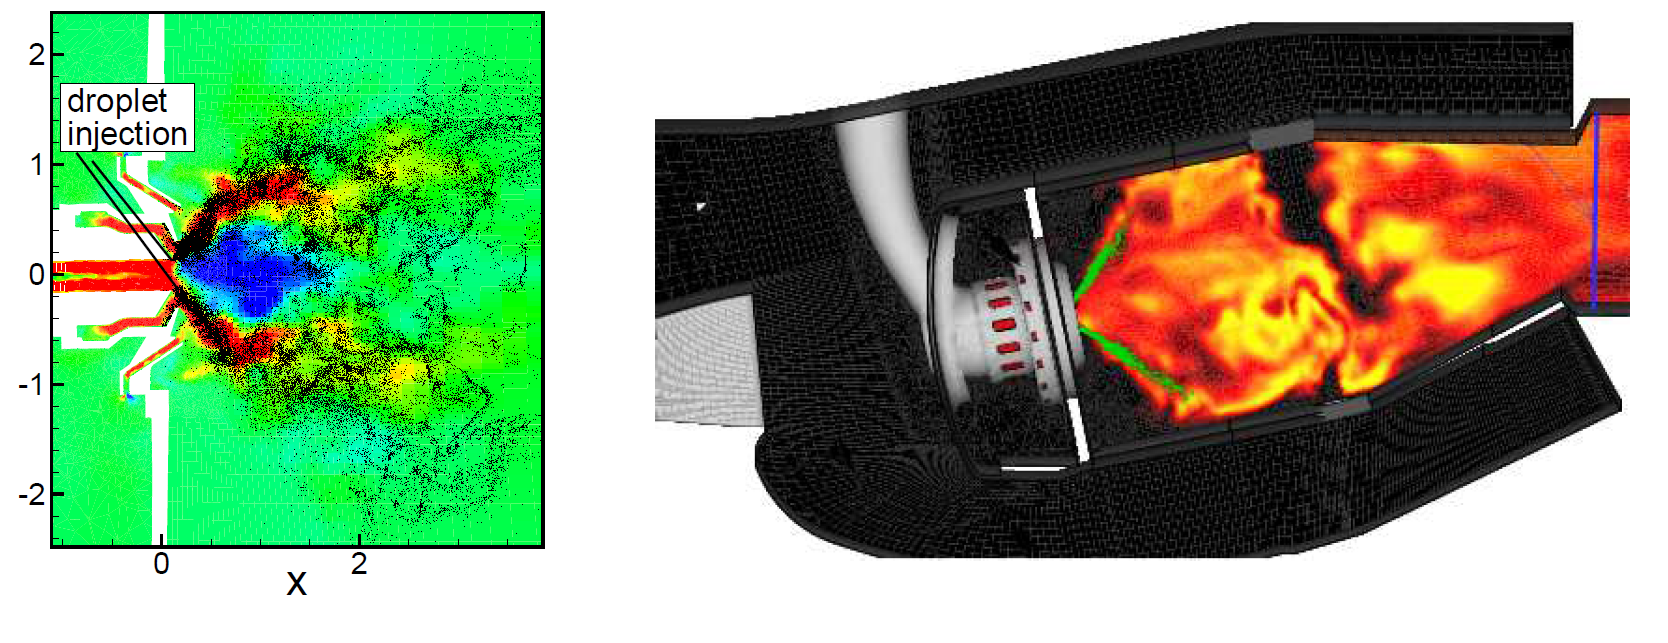
\includegraphics[scale=0.45]{./part0_intro/reactive_LES_combustor_Moin}
	\caption[Large Eddy Simulation of a Pratt \& Whitney combustor.]{Large Eddy Simulation of a Pratt \& Whitney combustor. \textsl{Left}: fuel spray injection, where liquid phase is represented by lagrangian droplets. \textsl{Right}: combustion simulation. Source: \citeColor[moin_large-eddy_2006].}
	\label{fig:reactive_LES_combustor_Moin}
\end{figure}

Recently, new methodologies have emerged to represent more accurately the spray by coupling dispersed phase with lagrangian simulations. \citeColor[michaelides_multiphase_2017] make a distinction of these coupling methodologies in two main categories: Direct Coupling Approach (DCA) and Statistical Coupling Approach (SCA), shown in Figure \ref{fig:coupled_EE_EL_approaches_Michaelides}. In DCA, primary atomization is simulated with eulerian approaches, and resolved eulerian droplets are transformed into spherical droplets which are later transported with the lagrangian equations. Conversion criteria based on droplets size and sphericity are used. This approach has been studied by several authors who have demonstrated its capabilities to simulate non-reactive problems \citemColor[herrmann_parallel_2010,zuzio_improved_2018], but has not yet been applied to combustion cases. In SCA, an eulerian simulation resolves the jet up to a plane after atomization has taken place where droplets are sampled (SC layer in Figure \ref{fig:coupled_EE_EL_approaches_Michaelides}). Then, the information on the sampled spray is used to inject lagrangian droplets, which are then transported further downstream.

\begin{figure}[h!]
	\centering
   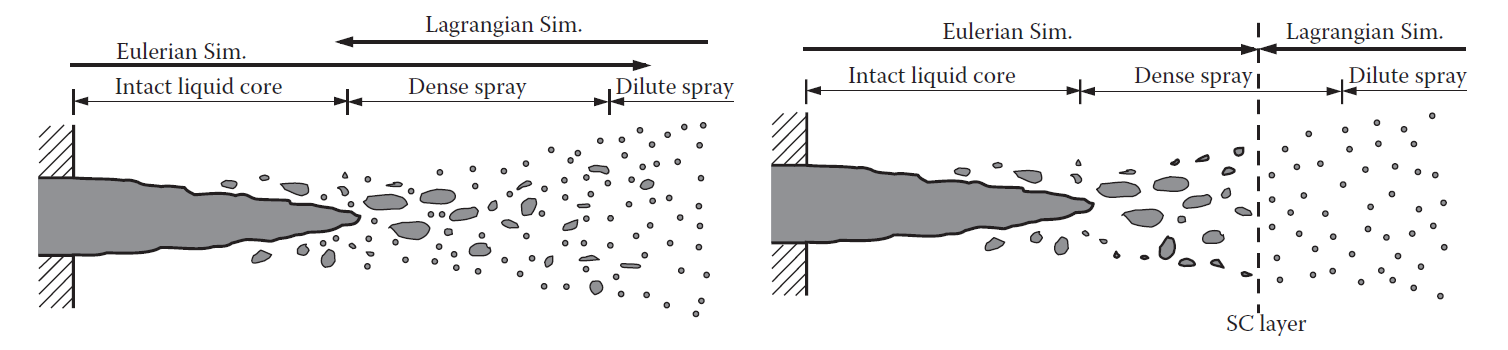
\includegraphics[scale=0.5]{./part0_intro/coupled_EE_EL_approaches_Michaelides}
	\caption[Schematic of coupled Eulerian–Lagrangian approaches for liquid atomization.]{Schematic of coupled Eulerian–Lagrangian approaches for liquid atomization. \textsl{Left}: direct coupling approach, DCA. \textsl{Right}: statistical coupling approach, SCA. Source: \citeColor[michaelides_multiphase_2017].}
	\label{fig:coupled_EE_EL_approaches_Michaelides}
	% Michaelides, p. 1140
\end{figure}


\section{Objective and thesis outline}
\label{sec:ch1_objective_thesis_outline}
    %\addcontentsline{toc}{section}{\protect\numberline{}Manuscript organisation}

The interest in performing lagrangian simulations to study combustion within gas turbines has seen a huge increase in the recent decades due to the potential of this methodology for modeling multi-physics problems with reduced computational costs. To accurately initialise perform such simulations, lagrangian particles needs to be properly injected by prescribing droplets sizes and velocities in the right spatial location. Often, distributions measured experimentally are in such simulations to recover the dispersed spray obtained further downstream. This requires, of course, the existence of experimental test benches which are representative of the geometry and operating conditions simulated, sometimes which is not always possible. Other approaches make use of simulations to obtain these distributions, which 



the injection process of lagrangian droplets needs to be properly modeled by introducing droplets sizes and velocities representative of the dispersed spray formed after at


    
The purpose of this thesis is to develop a new methodology to build lagrangian injectors for performing dispersed phase simulations. 

This thesis has been performed with Safran Group under the ITN programme ANNULIGhT, funded by the H2020 Marie Curie actions. The manuscript is divided in three main sections as follows:

\begin{itemize}

	\item \textbf{Part I} shows the state of the art in numerical methods to simulate two-phase flows. Different strategies are used depending on the atomization regimes as shown in Figure \ref{fig:atomization_regimes_herrmann}. Chapter \ref{ch2:numerical_methods_resolved_atomization} reviews methodologies aiming at resolving atomization, applicable to dense regimes and useful when the atomization dynamics need to be known, but out of scope for reactive simulations including combustion. Chapter \ref{ch3:disperse_phase_methods} discusses methodologies to simulate dispersed-phase problems, with a particular emphasis on the state of the art in lagrangian methodologies to simulate injection in MSI.
	
	\item \textbf{Part II} describes the design and application of the methodology developed in this thesis. This methodology is thoroughly described in Chapter . Then, application of this methodology to build lagrangian injectors in an academic non-reactive kerosene jet in crossflow test case is done in Chapter \ref{ch5:jicf_resolved_simulations}. The obtained injectors are then applied in the same configuration to initialise dispersed phase simulations in Chapter \ref{ch4:sli_development}.
	
	\item \textbf{Part III} focuses on the application of the injection models in an academic MSFI tested at EM2C named BIMER. An introduction to the test bench and simulations of the aerodynamic field are presented in Chapter \ref{ch9:bimer_test_bench_and_aero}. Then, Chapter \ref{ch8:bimer_resolved_atomization} describes resolved simulations of the atomization process in BIMER performed for one multipoint injector, from which lagrangian injectors are learnt. Finally, Chapter \ref{ch9:BIMER_lagrangian} shows the application of the learnt injectors to initialise lagrangian injection in the take-off stage of BIMER.

\end{itemize}


\newpage	

%----------- Part I: Numerical approaches --------------
\part{Numerical approaches to model injection systems}


\chapter{Numerical methods to simulate resolved atomization}
	\label{ch2:numerical_methods_resolved_atomization}

\section{Introduction}

\textbf{MAKE LINK WITH FINAL PART OF INTRODUCTION WHEN IT IS DONE}

Resolution of two-phase flows requires a suitable description of each phase and a careful treatment of the liquid-gas interface. From a numerical point of view, the multi-scale nature of atomization makes it impossible to use the same methods for resolving atomization accurately and for transporting a developed spray, since the characteristic length scales differ by several orders of magnitude. Consequently, different numerical methodologies must be chosen according to the targeted problem. Furthermore, if multi-physical phenomena, such as evaporation or combustion, are present, the range of possible models to be applied becomes even narrower.

The first step to choose a proper methodology is to identify the type of regime to solve. One possible classification of two-phase regimes can be done depending on the distribution and topology of the interface. In this respect, one can distinguish between separate and disperse phase \citepColor[murrone_numerical_2011]: 


%Suitable modeling strategies are needed to resolve a two-phase flow problem. The strategy chosen will depend on many things, such as the coherence of the liquid phase or the ambient conditions. Hence, the same strategies applied when studying injection at take-off conditions might not be the same than the ones required for relight  altitude relight problems, for example.

%A key challenge in two-phase flows is to resolve the fluid-gas interface and its evolution with space and time so that the atomization process can be properly described. Modeling the interface is not an easy task due to the difference in density and viscosity between both fluids, and several strategies have been developed to solve this issue. The scientific community classifies these models in two big families according to the liquid volume fraction contained within a given control volume. These two families are the \textbf{dense core} and the \textbf{disperse liquid phase} approaches:

%A general classification for two-phase flows systems can be done according to how both phases are separated \citepColor[murrone_numerical_2011], see Fig. :

\begin{itemize}

\item \textbf{Separate phase} flows, also known as dense regime, present a clear definition of the interface and both liquid and gaseous phases can be easily identified (Figure \ref{fig:TPF_droplets_example} left). In such cases, the liquid volume fraction is large and the liquid structures are of the same order, or larger, than the cell size, so the atomization dynamics can be captured by the mesh. Within engines, separate phase is found during primary breakup, as shown by the blue regions of Fig. \ref{fig:atomization_regimes_herrmann}. Numerical methods devoted to resolve separate phase regimes are tackled in this chapter ($\S$\ref{sec:ch2_eulerian_approaches_dense_regime}). Generally, these methods are restricted to non-reactive problems and the multi-physics coupling with evaporation and combustion is not possible.

\item \textbf{Dispersed phase} regime is found when the liquid volume fraction is small and the liquid structures cannot be capture by the main grid. The liquid phase is composed by individual liquid particles (usually called droplets) whose high number and small size hinders the tracking of the interface (Figure \ref{fig:TPF_droplets_example} right). Droplets are surrounded by the gaseous phase, also called \textbf{carrier phase}. A developed spray produced as a consequence of secondary atomization is an example of dispersed phase systems, illustrated by the intermediate and dilute regimes of Figure \ref{fig:atomization_regimes_herrmann}. The same numerical methods used for the separate phase regime cannot be applied, since the characteristic scales are much smaller and the grid resolution required yields the computations unaffordable due to their high cost. Numerical formalisms targeting dispersed phase flows are discussed in Chapter \ref{ch3:disperse_phase_methods}. These methods do not resolve atomization as accurately as the ones employed for separate phases, but present the possibility to integrate evaporation and combustion.

\end{itemize}

\begin{figure}[h!]	
	\centering
	\includeinkscape[inkscapelatex=false,scale=0.75]{./part1_numerical_approaches/figures_ch2/TPF_approaches_example}
	\caption{Two-phase systems classification. \textsl{Left}: separate flow, where both phases are easily distinguished and the interface $\Gamma$ can easily be tracked. \textsl{Right}: dispersed phase flow, where individual fluid particles (disperse phase) are surrounded by the gas (carrier phase). In such systems, the interface can hardly be tracked due to the higher surface-to-volume ratio.}
	\label{fig:TPF_droplets_example}
\end{figure}

%Different numerical models have been developed to solve two-phase flows. Due to the differences aforementioned, each method will target problems involving mainly either separate or disperse phase. Volume of fluid ($\S$\ref{subsec:ch2_VOF}) or level-set ($\S$\ref{subsec:ch2_ACLS}) methods are suitable for solving primary atomization, but becomes inefficient when applying it to a cluster of small particles product of secondary atomization. Lagrangian methods, dealt in Chapter \ref{ch3:disperse_phase_methods}, are suitable to represent disperse phase systems containing droplets moving individually, but cannot properly represent a dense liquid region with high volume fraction and would need extra modeling to represent the physics more accurately \citepColor[reitz_modeling_1987].

An \colorbox{red}{insightful} classification of existing numerical methods for two-phase flows is shown in Figure \ref{fig:classification_numerical_methods_mirjalili}. Methods aiming at solving disperse-phase flows use often a two-fluid formulation, since the description of each phase is often done with separate equations. On the other hand, methods addressing separate phases are based on a one-fluid formulation, since basically the same governing equations are solved but distinguishing between phases via their different physical properties. This requires a specific treatment of the interface and the jump conditions in pressure due to surface tension, which each method will handle differently. 

This chapter gives an overview on the state-of-the-art in numerical methods applicable to resolve separate phase regimes. Section \ref{sec:ch2_governing_equations} introduces the governing equations of non-reactive two phase flows, beginning by introducing the Reynolds Transport Theorem and applying it to obtain mass and momentum conservation laws. Section \ref{sec:ch2_eulerian_approaches_dense_regime} presents the numerical methodologies reviewed: diffuse interface, front-tracking, Volume of Fluid (VOF), and Accurate Conservative Level-Set coupled with Ghost-Fluid Method (ACLS/GMF). The last one is the methodology used in this thesis for performing resolved simulation atomizations in Chapter \ref{ch5:jicf_resolved_simulations}.


\begin{figure}[h!]
	\centering
	\includegraphics[scale=1.0]{./part1_numerical_approaches/figures_ch2/classification_numerical_methods_mirjalili}
	\caption{Numerical methods to simulate two-phase flows. Ellipses denote interface-capturing methods. Sharp-interface methods are denoted by a white background, while the grey one indicates diffuse-interface methods. Source: \citeColor[mirjalili_interface-capturing_2017]}
	\label{fig:classification_numerical_methods_mirjalili}
\end{figure}

%Figure \ref{fig:classification_numerical_methods_mirjalili} depicts another classification of methods for two-phase flows according to how they see the interface: \textbf{sharp interface} (white background boxes) and \textbf{diffuse interface} (grey background). The former, as their name indicates, identify the interface as a diffused spatial region where both phases coexists. Diffuse-interface methods are succinctly presented in $\S{subsec:ch2_DI_methods}$. Sharp interface methods, some of which are presented in later sections, see the interface as an infinitely-thin front moving at a certain speed. Hence, the interface is located at a given value of a scalar function which is advected by the fluid. 


\section{Governing equations }
\label{sec:ch2_governing_equations}

\subsection{Reynolds transport theorem}

\subsubsection*{General form}

The starting point for deriving all the conservation equations is the Reynolds transport theorem (RTT). Let's consider a control volume $\Omega$ bounded by a control surface $\partial \Omega$. Let's also consider a control mass $\Omega_m$ which moves with time to enclose the same amount of mass. This control mass coincides at some time instant with the control volume. The RTT relates the variation of a property $\phi = \phi \left( \boldsymbol{x}, t \right)$ in the control mass with its variation in the control volume. In its most general form, it can be expressed as follows \citepColor[collado_reynolds_2007]:

\begin{equation}
\label{eq:RTT_more_general_shape}
\frac{d}{dt} \int_{\Omega_m} \phi  dV =  \frac{ d}{dt} \int_\Omega \phi dV + \int_{\partial \Omega} \phi  \left( \boldsymbol{u} - \boldsymbol{u_c} \right) \cdot \boldsymbol{n}  dS
\end{equation}

where $\boldsymbol{u}$ is the flow velocity at the boundaries, $\boldsymbol{u_c}$ is the velocity of the control surface and $\boldsymbol{n}$ is the normal unit vector pointing outwards the surface of the control volume. Bold symbols indicate vectorial quantities. 

The first term in the right hand side can be expanded by applying Leibniz's integral rule to a domain with moving boundaries. Following the introduced notation, Leibniz's rule takes the following shape:

\begin{equation}
\label{eq:reynolds_transport_theorem_general_controlVolume}
\frac{d}{dt} \int_\Omega \phi dV =  \int_\Omega \frac{\partial \phi}{\partial t} dV + \int_{\partial \Omega} \phi \left( \boldsymbol{u_c} \cdot \boldsymbol{n} \right) dS
\end{equation}

The latter equation can also be seen as another expression for the RTT particularised for a moving control volume. Introducing it into (\ref{eq:RTT_more_general_shape}) yields:


\begin{equation}
\label{eq:reynolds_transport_theorem_general_controlMass}
\boxed{
\frac{d}{dt} \int_{\Omega_m} \phi  dV = \int_\Omega \frac{\partial \phi}{\partial t} dV + \int_{\partial \Omega} \phi   \left( \boldsymbol{u} \cdot \boldsymbol{n} \right) dS
}
\end{equation}

This formulation of the relates the lagrangian formulation of a system (left hand side, corresponding to the control mass) with the eulerian formulation (right hand side, corresponding to the control volume). 

In this document all the control volumes selected for performing balances will be fixed in space, so their boundaries not move. Consequently, $\boldsymbol{u_c} = 0$ and hence Eq. (\ref{eq:reynolds_transport_theorem_general_controlVolume}) becomes $\frac{d}{dt} \int_\Omega \phi dV =  \int_\Omega \partial \phi/\partial t ~ dV$.

\subsubsection*{Application to two-phase flows}
	\label{subsec:RTT_applied_to_TPS_with_interface}

In the particular case of two-phase flows systems comprising gas and liquid phases, denoted respectively by the subscripts $g$ and $l$, the domain can be decomposed into two subdomains $\Omega_\mathrm{g}$ and $\Omega_\mathrm{l}$. The addition of these two subdomains will make the total domain $\Omega$:

\begin{equation}
\label{eq:omega_domain_partition}
\Omega = \Omega_\mathrm{g} \cup \Omega_\mathrm{l}
\end{equation}

The RTT must hold for each subdomain, so Eq. (\ref{eq:reynolds_transport_theorem_general_controlMass}) can be applied to each phase separately

\begin{subequations}
\begin{align}
\frac{d}{dt} \int_{\Omega_{m_\mathrm{g}}} \phi ~ dV &=  \int_{\Omega_\mathrm{g}} \frac{\partial \phi}{\partial t} ~ dV + \int_{\partial \Omega_\mathrm{g}} \phi \left( \boldsymbol{u} \cdot \boldsymbol{n} \right) dS\\
\frac{d}{dt} \int_{\Omega_{m_\mathrm{l}}} \phi ~ dV &=  \int_{\Omega_\mathrm{l}} \frac{\partial \phi}{\partial t} ~ dV + \int_{\partial \Omega_\mathrm{l}} \phi \left( \boldsymbol{u} \cdot \boldsymbol{n} \right) dS
\end{align}
\end{subequations}

The surface integral in the right hand side can be decomposed in two different integrals by considering a common boundary shared by both subdomains: the liquid-gas interface $\Gamma$. This interface can be modified with time. Hence, the control boundary $\partial \Omega$ can be expressed as the addition of the following two subdomains:

\begin{equation}
\label{eq:partial_omega_boundaries_partition}
\partial \Omega = \left( \partial \Omega_\mathrm{g} \backslash \Gamma ~ \right) \cup \left( \partial \Omega_\mathrm{l} \backslash \Gamma ~ \right)
\end{equation}

So the RTT for separate phases can be extended as follows:


\begin{subequations}
\begin{align}
\frac{d}{dt} \int_{\Omega_{m_\mathrm{g}}} \phi ~ dV &=  \int_{\Omega_\mathrm{g}} \frac{\partial \phi}{\partial t} ~ dV + \int_{\partial \Omega_\mathrm{g} \backslash \Gamma} \phi \left( \boldsymbol{u} \cdot \boldsymbol{n} \right) dS + \int_{\Gamma} \phi_\mathrm{g} \left( \boldsymbol{u}_{\scriptsize{\Gamma}} \cdot {\boldsymbol{n}_{\scriptsize{\Gamma}}}_\mathrm{g} \right) dS \\
\frac{d}{dt} \int_{\Omega_{m_\mathrm{l}}} \phi ~ dV &=  \int_{\Omega_\mathrm{l}} \frac{\partial \phi}{\partial t} ~ dV + \int_{\partial \Omega_\mathrm{l} \backslash \Gamma} \phi \left( \boldsymbol{u} \cdot \boldsymbol{n} \right) dS + \int_{\Gamma} \phi_\mathrm{l} \left( \boldsymbol{u}_{\scriptsize{\Gamma}} \cdot {\boldsymbol{n}_{\scriptsize{\Gamma}}}_\mathrm{l} \right) dS
\end{align}
\end{subequations}

where $\boldsymbol{u}_{\scriptsize{\Gamma}}$ is the velocity at the interface and $\boldsymbol{n}_{\scriptsize{\Gamma}}$ is the vector normal to the interface pointing outwards its corresponding phase. As the interface is the same but the outward direction is opposed for each phase, an interface normal vector pointing to the liquid phase can be defined: 

\begin{equation}
\boldsymbol{n}_{\scriptsize{\Gamma}} = {\boldsymbol{n}_{\scriptsize{\Gamma}}}_\mathrm{l} = - {\boldsymbol{n}_{\scriptsize{\Gamma}}}_\mathrm{g}
\end{equation}

Hence, the RTT for each separate phase can be reformulated as:

\begin{subequations}
\label{eq:RTT_general_twoEquations}
\begin{align}
\frac{d}{dt} \int_{\Omega_{m_\mathrm{g}}} \phi ~ dV &=  \int_{\Omega_\mathrm{g}} \frac{\partial \phi}{\partial t} ~ dV + \int_{\partial \Omega_\mathrm{g} \backslash \Gamma} \phi \left( \boldsymbol{u} \cdot \boldsymbol{n} \right) dS - \int_{\Gamma} \phi_\mathrm{g} \left( \boldsymbol{u}_{\scriptsize{\Gamma}} \cdot \boldsymbol{n}_{\scriptsize{\Gamma}} \right) dS \\
\frac{d}{dt} \int_{\Omega_{m_\mathrm{l}}} \phi ~ dV &=  \int_{\Omega_\mathrm{l}} \frac{\partial \phi}{\partial t} ~ dV + \int_{\partial \Omega_\mathrm{l} \backslash \Gamma} \phi \left( \boldsymbol{u} \cdot \boldsymbol{n} \right) dS + \int_{\Gamma} \phi_\mathrm{l} \left( \boldsymbol{u}_{\scriptsize{\Gamma}} \cdot \boldsymbol{n}_{\scriptsize{\Gamma}}\right) dS
\end{align}
\end{subequations}

Finally, a general shape for the RTT in two-phase flows can be obtained by adding Equations (\ref{eq:RTT_general_twoEquations}) and applying (\ref{eq:omega_domain_partition}) and (\ref{eq:partial_omega_boundaries_partition}):

\begin{equation}
\label{eq:RTT_general_bothPhases}
\frac{d}{dt} \int_{\Omega_m} \phi dV =  \int_{\Omega} \frac{\partial \phi}{\partial t}  dV + \int_{\partial \Omega} \phi \left( \boldsymbol{u} \cdot \boldsymbol{n} \right) dS + \int_\mathsmaller{\Gamma} \left( \phi_\mathrm{l} - \phi_\mathrm{g} \right) \left( \boldsymbol{u}_{\scriptsize{\Gamma}} \cdot \boldsymbol{n}_{\scriptsize{\Gamma}} \right) dS
\end{equation}





\subsection{Mass conservation}

\subsubsection*{General forms}

The mass conservation equation for a fluid system is obtained by substituting $\phi = \rho$ in Eq. (\ref{eq:reynolds_transport_theorem_general_controlMass}):

\begin{equation}
\frac{d}{dt} \int_{\Omega_m} \rho  dV =  \int_\Omega \frac{\partial \rho}{\partial t} dV + \int_{\partial \Omega} \rho \boldsymbol{u} \cdot \boldsymbol{n} dS
\end{equation}

By definition, the control mass is a region of the fluid flow whose mass does not change. Hence, the left hand side of the previous expression is $0$ and the \textbf{mass conservation in integral form}, or \textbf{weak form of mass conservation}, is expressed as follows:


\begin{equation}
\label{eq:mass_conservation_general_integral}
\boxed{
\int_\Omega \frac{\partial \rho}{\partial t}   dV + \int_{\partial \Omega} \rho \boldsymbol{u} \cdot \boldsymbol{n} dS = 0
}
\end{equation}

The Gauss theorem can be applied to a vectorial field $\boldsymbol{f}$ to transform a surface integral into a volume integral:

\begin{equation}
\label{eq:gauss_theorem}
\int_{\partial \Omega} \boldsymbol{f} \cdot \boldsymbol{n} dS = \int_\Omega \nabla \boldsymbol{f}  dV
\end{equation}

Applying this theorem considering $\boldsymbol{f} = \rho \boldsymbol{u}$ and substituting into (\ref{eq:mass_conservation_general_integral}) yields the general expression for \textbf{mass conservation in differential form} or \textbf{strong form of mass conservation}:

\begin{equation}
\label{eq:mass_conservation_general_differential}
\boxed{
\frac{\partial \rho}{\partial t} + \nabla \left( \rho \boldsymbol{u} \right) = 0
}
\end{equation}

This equation is also known as the \textbf{continuity equation in conservative form}. The \textbf{non-conservative} form can be obtained by expanding the left-hand side:

\begin{equation}
\frac{\partial \rho}{\partial t} + \nabla \left( \rho \boldsymbol{u} \right) = \frac{\partial \rho}{\partial t} + \boldsymbol{u} \cdot \nabla \rho  + \rho \nabla \boldsymbol{u} = 0 ~~~~ \rightarrow ~~~~ \frac{d \rho}{d t} + \rho \nabla \boldsymbol{u} = 0
\end{equation}

where $d / d t = \partial / \partial t + \boldsymbol{u} \cdot \nabla $ is the \textbf{material derivative}. 

Hereafter, the weak form of mass conservation will be addressed for its application in integral balances.

\subsubsection*{Global mass conservation in two-phase flows}

A global expression for mass conservation can be obtained by substituting $\phi = \rho$ into Eq. (\ref{eq:RTT_general_bothPhases}):

\begin{equation}
\frac{d}{dt} \int_{\Omega_m} \rho dV =   \int_{\Omega}  \frac{\partial \rho}{\partial t}  dV + \int_{\partial \Omega} \rho \boldsymbol{u} \cdot \boldsymbol{n} dS + \int_\mathsmaller{\Gamma} \left( \rho_\mathrm{l} - \rho_\mathrm{g} \right) \left( \boldsymbol{u}_{\scriptsize{\Gamma}} \cdot \boldsymbol{n}_{\scriptsize{\Gamma}} \right) dS
\end{equation}

In conditions where mass exchange takes place, such as the hot environment within combustion chambers, high temperature might produce evaporation of the liquid phase into gaseous phase. In such cases, the left hand side term of the former equation would be a sink term different to zero. However in this work mass exchange is not considered, so this term is zero:

\begin{equation}
\int_{\Omega}  \frac{\partial \rho}{\partial t}  dV + \int_{\partial \Omega} \rho \boldsymbol{u} \cdot \boldsymbol{n} dS + \int_\mathsmaller{\Gamma} \left( \rho_\mathrm{l} - \rho_\mathrm{g} \right) \left( \boldsymbol{u}_{\scriptsize{\Gamma}} \cdot \boldsymbol{n}_{\scriptsize{\Gamma}}\right) dS = 0
\end{equation}

It can be noticed that the first two integrals in this expression correspond to the weak form for mass conservation as given by Eq. (\ref{eq:mass_conservation_general_integral}). Hence, this expression is simplified to:

\begin{equation}
\int_\mathsmaller{\Gamma} \left( \rho_\mathrm{l} - \rho_\mathrm{g} \right) \left( \boldsymbol{u}_{\scriptsize{\Gamma}} \cdot \boldsymbol{n}_{\scriptsize{\Gamma}} \right) dS = 0
\end{equation}

As both $\rho_\mathrm{l}$ and $\rho_\mathrm{g}$ are always positive, and $\rho_\mathrm{l} > \rho_\mathrm{g}$ for most known applications (including gas turbines and atmospheric two-phase systems), the only possibility for this expression to hold true is when the dot product is zero:

\begin{equation}
\label{eq:continuity_TPF_noFluxThroughInterface}
\boxed{
\boldsymbol{u}_{\scriptsize{\Gamma}} \cdot \boldsymbol{n}_{\scriptsize{\Gamma}} = 0
}
\end{equation}

which means that the flow velocity normal to the interface must be zero, i.e. there is no liquid or gas crossing the interface. 

\subsubsection*{Mass conservation in separate phases}
	\label{eq:mass_conservation_separated_phases}

Two-phase flows must ensure mass conservation for each phase. This can be done by applying the RTT as given by Eqs. (\ref{eq:RTT_general_twoEquations}) to the field $\phi = \rho$. However this formulation introduces the need to deal with the liquid-gas interface, which is often changing in time. A more useful formulation can be developed by the strong form given by (\ref{eq:mass_conservation_general_integral}) to each phase separately \citepColor[drew_theory_1999]. For making it properly, it is necessary to introduce before the definition of \textbf{volumetric fraction} for a phase $k$, $\alpha_k$:

\begin{equation}
\alpha_k = \frac{V_k}{V}
\end{equation}

This magnitude determines the quantity of a given fluid $k$ that is contained in a considered volume $V$. By definition, it follows that $\sum_{k=1}^\mathrm{N_{phases}} \alpha_k = 1$. It can be defined for both gas and liquid phases, $\alpha_\mathrm{g}$ and $\alpha_\mathrm{l}$, so then $\alpha_\mathrm{g} + \alpha_\mathrm{l} = 1$.

Once the volumetric fractions for liquid and gas have been defined, the continuity equation (\ref{eq:mass_conservation_general_differential}) can be defined for each phase as follows:

\begin{subequations}
\begin{align}
\frac{\partial \alpha_\mathrm{g} \rho_\mathrm{g} }{\partial t} + \nabla \left( \alpha_\mathrm{g} \rho_\mathrm{g} \boldsymbol{u}_\mathrm{g} \right) &= 0  \\
\frac{\partial \alpha_\mathrm{l} \rho_\mathrm{l} }{\partial t} + \nabla \left( \alpha_\mathrm{l} \rho_\mathrm{l} \boldsymbol{u}_\mathrm{l} \right) &= 0
\end{align}
\end{subequations}

The integral balance can be obtained by integrating both expressions over a fixed control volume $\Omega$ and applying the Gauss theorem to the divergence term:

\begin{subequations}
\label{eq:mass_conservation_general_bothPhases_showingIntegrals}
\begin{align}
\frac{\partial}{\partial t} \int_{\Omega} \alpha_\mathrm{g} \rho_\mathrm{g} dV + \int_{\partial {\Omega}} \alpha_\mathrm{g} \rho_\mathrm{g} \left( \boldsymbol{u}_\mathrm{g} \cdot \boldsymbol{n} \right) dS &= 0  \\
\frac{\partial}{\partial t} \int_{\Omega} \alpha_\mathrm{l} \rho_\mathrm{l} dV + \int_{\partial {\Omega}} \alpha_\mathrm{l} \rho_\mathrm{l} \left( \boldsymbol{u}_\mathrm{l} \cdot \boldsymbol{n} \right) dS &= 0 
\end{align}
\end{subequations}

These equations present two components: a transient term and a surface term. The transient term has an effect when the mass of any phase is growing inside the control volume, e.g. at the first instants of fuel injection, when the fuel mass is increasing with time. Once a steady-state has been reached, this term becomes $0$. The surface term accounts for the mass fluxes that are entering of leaving the system through its boundaries. From this term, the \textbf{mass flow rate} $\dot{m}$ of a flux going though an area $A$ can be defined as:

\begin{equation}
\boxed{
\label{eq:mass_flow_rate_definition_general}
\dot{m} = \int_A \rho \left( \boldsymbol{u} \cdot \boldsymbol{n} \right) dS
}
\end{equation}

An inspection of this equation reveals a dot product between the velocity vector and the normal vector to the surface. As the normal vector is pointing outwards the control volume, the dot product will be positive in surfaces where both vectors have the same direction, and negative otherwise. Hence, the mass flow rate will be positive in outlets and negative in inlets.

If the transient term in (\ref{eq:mass_conservation_general_bothPhases_showingIntegrals}), which is a source term, is denoted as $\dot{\Omega}_m$, then the mass conservation for separated phases can be written as follows:

\begin{subequations}
\begin{align}
\dot{\Omega}_{m_\mathrm{g}} + \sum_i \dot{m}_{g_i} &= 0  \\
\dot{\Omega}_{m_\mathrm{l}} + \sum_j \dot{m}_{l_j} &= 0 
\end{align}
\end{subequations}

Considering that inlet fluxes are negative and outlet fluxes are positive, the equations can be rearranged:

\begin{subequations}
\label{eq:mass_conservation_general_bothPhases_transient}
\begin{empheq}[box=\fbox]{align}
\dot{\Omega}_{m_\mathrm{g}} &= \sum_{i_\mathrm{in}} \dot{m}_{g_i} - \sum_{i_\mathrm{out}} \dot{m}_{g_i}  \\
\dot{\Omega}_{m_\mathrm{l}} &= \sum_{j_\mathrm{in}} \dot{m}_{l_j} - \sum_{j_\mathrm{out}} \dot{m}_{l_j}
\end{empheq}
\end{subequations}

\subsection{Momentum conservation}

\subsubsection*{General forms}

The momentum conservation equation for a fluid system is obtained by substituting $\phi = \rho \boldsymbol{u}$ in Eq. (\ref{eq:reynolds_transport_theorem_general_controlMass}):

\begin{equation}
\frac{d}{dt} \int_{\Omega_m} \rho \boldsymbol{u}  dV =  \int_\Omega \frac{\partial \left( \rho \boldsymbol{u} \right) }{\partial t} dV + \int_{\partial \Omega} \rho \boldsymbol{u} \left( \boldsymbol{u} \cdot \boldsymbol{n} \right) dS
\end{equation}

The left-hand side term represents the ensemble of forces acting in the control mass. These forces can be separated into volume and surface forces. The volume forces will be denoted by $\boldsymbol{b}$; the surface forces include the pressure $p$ and the viscous stress tensor $\overline{\overline{\pmb{\tau}}}$. With this notation, the \textbf{momentum conservation in integral form}, or \textbf{weak form of momentum conservation}, is defined as:

\begin{equation}
\label{eq:momentum_conservation_general_integral}
\boxed{
\int_\Omega \frac{\partial \left( \rho \boldsymbol{u} \right) }{\partial t} dV + \int_{\partial \Omega} \rho \boldsymbol{u} \left( \boldsymbol{u} \cdot \boldsymbol{n} \right) dS =  \int_{\partial \Omega} \left( - p \overline{\overline{\pmb{I}}} + \overline{\overline{\pmb{\tau}}} \right) \boldsymbol{n} dS + \int_\Omega \boldsymbol{b} dV
}
\end{equation}

where $\overline{\overline{\pmb{I}}}$ is the identity matrix. Applying the Gauss theorem (\ref{eq:gauss_theorem}) with $\boldsymbol{f} = \rho \boldsymbol{u} \boldsymbol{u}$ and operating yields the \textbf{momentum conservation in differential form}, or \textbf{strong form of momentum conservation}:

\begin{equation}
\label{eq:momentum_conservation_general_differential}
\boxed{
\frac{\partial \left( \rho \boldsymbol{u} \right) }{\partial t}  + \nabla \left( \rho \boldsymbol{u}  \boldsymbol{u} \right) =  - \nabla p + \nabla \overline{\overline{\pmb{\tau}}} + \boldsymbol{b} 
}
\end{equation}

This solution is also known as the \textbf{conservative form of the momentum equation}. The left-hand side can be further expanded:

\begin{equation}
\frac{\partial \left( \rho \boldsymbol{u} \right) }{\partial t}  + \nabla \left( \rho \boldsymbol{u}  \boldsymbol{u} \right) =  \boldsymbol{u} \underbrace{ \left[ \frac{\partial \rho}{\partial t} +  \nabla \left( \rho \boldsymbol{u} \right) \right]}_{\text{Continuity}\atop\text{equation (\ref{eq:mass_conservation_general_differential})}}  + \rho \left[ \frac{\partial \boldsymbol{u}}{\partial t} +  \boldsymbol{u} \cdot \nabla \boldsymbol{u} \right] = \rho \left( \frac{\partial \boldsymbol{u}}{\partial t} +  \boldsymbol{u} \cdot \nabla \boldsymbol{u} \right) = \rho \frac{d \boldsymbol{u}}{dt}
\end{equation}

%% Intermediate step:
% \rho \frac{\partial \boldsymbol{u}}{\partial t} + \boldsymbol{u} \frac{\partial \rho}{\partial t} + \rho \boldsymbol{u} \nabla \boldsymbol{u} + \boldsymbol{u} \nabla \left( \rho \boldsymbol{u} \right)

With this notation, the \textbf{non-conservative form} is obtained:

\begin{equation}
\rho \frac{d \boldsymbol{u}}{dt} =  - \nabla p + \nabla \overline{\overline{\pmb{\tau}}} +  \boldsymbol{b} 
\end{equation}


\subsubsection*{Global momentum conservation in two-phase flows}

A global expression for momentum conservation can be obtained by substituting $\phi = \rho \boldsymbol{u}$ into Eq. (\ref{eq:RTT_general_bothPhases}):

\begin{equation}
\frac{d}{dt} \int_{\Omega_m} \rho \boldsymbol{u} dV =   \int_{\Omega}  \frac{\partial \rho \boldsymbol{u} }{\partial t}  dV + \int_{\partial \Omega} \rho \boldsymbol{u} \left( \boldsymbol{u} \cdot \boldsymbol{n} \right) dS + \int_\mathsmaller{\Gamma} \left( \rho_\mathrm{l} \boldsymbol{u}_\mathrm{l} - \rho_\mathrm{g} \boldsymbol{u}_\mathrm{g} \right) \left( \boldsymbol{u}_{\scriptsize{\Gamma}} \cdot \boldsymbol{n}_{\scriptsize{\Gamma}} \right) dS
\end{equation}

The left-hand side term can be expressed in the same way as in Eq. (\ref{eq:momentum_conservation_general_integral}) with a slight modification: another addend must be included to account for the interface, as done in $\S$\ref{subsec:RTT_applied_to_TPS_with_interface}. In this way, this term becomes:

\begin{equation}
\frac{d}{dt} \int_{\Omega_m} \rho \boldsymbol{u} dV =  \int_{\partial \Omega} \left( - p \overline{\overline{\pmb{I}}} + \overline{\overline{\pmb{\tau}}} \right) \boldsymbol{n} dS + \int_\Omega \boldsymbol{b} dV + \int_{\Gamma} \left[ - \left( p_\mathrm{l} - p_\mathrm{g} \right) \overline{\overline{\pmb{I}}} + \left( \overline{\overline{\pmb{\tau}}}_\mathrm{l} - \overline{\overline{\pmb{\tau}}}_\mathrm{g}  \right) + \overline{\overline{\pmb{\tau}}}_\sigma  \right] \boldsymbol{n} dS
\end{equation}

In the interface term, a new contribution has been added: surface tension, represented in this equation by the tensor $\overline{\overline{\pmb{\tau}}}_\sigma$. Surface tension only contributes in the interface. These terms can now be introduced in the momentum conservation equation:

\begin{multline}
 \int_{\Omega}  \frac{\partial \rho \boldsymbol{u} }{\partial t}  dV + \int_{\partial \Omega} \rho \boldsymbol{u} \left( \boldsymbol{u} \cdot \boldsymbol{n} \right) dS + \int_\mathsmaller{\Gamma} \left( \rho_\mathrm{l} \boldsymbol{u}_\mathrm{l} - \rho_\mathrm{g} \boldsymbol{u}_\mathrm{g} \right) \left( \boldsymbol{u}_{\scriptsize{\Gamma}} \cdot \boldsymbol{n}_{\scriptsize{\Gamma}} \right) dS = \\ = \int_{\partial \Omega} \left( - p \overline{\overline{\pmb{I}}} + \overline{\overline{\pmb{\tau}}} \right) \boldsymbol{n} dS + \int_\Omega \boldsymbol{b} dV + \int_{\Gamma} \left( - \left( p_\mathrm{l} - p_\mathrm{g} \right) \overline{\overline{\pmb{I}}} + \left( \overline{\overline{\pmb{\tau}}}_\mathrm{l} - \overline{\overline{\pmb{\tau}}}_\mathrm{g}  \right) + \overline{\overline{\pmb{\tau}}}_\sigma  \right) \boldsymbol{n} dS
\end{multline}

Inspecting this equation reveals that the first two terms in both sides make the general integral form of momentum conservation, Eq. (\ref{eq:momentum_conservation_general_integral}). Therefore, the equation can be simplified:

\begin{equation}
\int_\mathsmaller{\Gamma} \left( \rho_\mathrm{l} \boldsymbol{u}_\mathrm{l} - \rho_\mathrm{g} \boldsymbol{u}_\mathrm{g} \right) \left( \boldsymbol{u}_{\scriptsize{\Gamma}} \cdot \boldsymbol{n}_{\scriptsize{\Gamma}} \right) dS =  \int_{\Gamma} \left( - \left( p_\mathrm{l} - p_\mathrm{g} \right) \overline{\overline{\pmb{I}}} + \left( \overline{\overline{\pmb{\tau}}}_\mathrm{l} - \overline{\overline{\pmb{\tau}}}_\mathrm{g}  \right) + \overline{\overline{\pmb{\tau}}}_\sigma  \right) \boldsymbol{n} dS
\end{equation}

By continuity in two phase flow, it was shown that $\boldsymbol{u}_{\scriptsize{\Gamma}} \cdot \boldsymbol{n}_{\scriptsize{\Gamma}} = 0$ in Eq.  (\ref{eq:continuity_TPF_noFluxThroughInterface}). Hence the left hand side is zero:

\begin{equation}
\int_{\Gamma} \left( - \left( p_\mathrm{l} - p_\mathrm{g} \right) \overline{\overline{\pmb{I}}} + \left( \overline{\overline{\pmb{\tau}}}_\mathrm{l} - \overline{\overline{\pmb{\tau}}}_\mathrm{g}  \right) + \overline{\overline{\pmb{\tau}}}_\sigma  \right) \boldsymbol{n} dS = 0
\end{equation}

From this relation, it directly follows that:

\begin{equation}
\boxed{
\left( p_\mathrm{l} - p_\mathrm{g} \right) \overline{\overline{\pmb{I}}} = \left( \overline{\overline{\pmb{\tau}}}_\mathrm{l} - \overline{\overline{\pmb{\tau}}}_\mathrm{g}  \right) + \overline{\overline{\pmb{\tau}}}_\sigma  
}
\end{equation}

As shown by this relation, the effect of surface tension it to introduce a discontinuity in pressure and viscous effects in the interface. 

\subsubsection*{Momentum conservation in separate phases}

Following the same procedure of $\S$\ref{eq:mass_conservation_separated_phases}, the volumetric fraction is used to formulate momentum equations in strong form. Equation (\ref{eq:momentum_conservation_general_differential}) can be applied to each phase for getting separate conservation equations of momentum. However, it must be taken into account that there can be exchange of momentum from one phase to another, something which was not taken into account in the mass equations because it is assumed that there is no mass exchange. This \textbf{momentum exchange} between both phases can be accounted for by adding a source term $\dot{\boldsymbol{s}}$. Then, the strong form of momentum conservation equations for each phase take the following form:

\begin{subequations}
\begin{align}
\frac{\partial \left( \alpha_\mathrm{g} \rho_\mathrm{g} \boldsymbol{u}_\mathrm{g} \right) }{\partial t}  + \nabla \left( \alpha_\mathrm{g} \rho_\mathrm{g} \boldsymbol{u}_\mathrm{g}  \boldsymbol{u}_\mathrm{g} \right) &=  - \nabla \left( \alpha_\mathrm{g} p_\mathrm{g} \right) + \nabla \left( \alpha_\mathrm{g} \overline{\overline{\pmb{\tau}}}_\mathrm{g} \right) + \alpha_\mathrm{g} \boldsymbol{b}_\mathrm{g} + \dot{\boldsymbol{s}}_\mathrm{g} \\
\frac{\partial \left( \alpha_\mathrm{l} \rho_\mathrm{l} \boldsymbol{u}_\mathrm{l} \right) }{\partial t}  + \nabla \left( \alpha_\mathrm{l} \rho_\mathrm{l} \boldsymbol{u}_\mathrm{l}  \boldsymbol{u}_\mathrm{l} \right) &=  - \nabla \left( \alpha_\mathrm{l} p_\mathrm{l} \right) + \nabla \left( \alpha_\mathrm{l} \overline{\overline{\pmb{\tau}}}_\mathrm{l} \right) + \alpha_\mathrm{l} \boldsymbol{b}_\mathrm{l} + \dot{\boldsymbol{s}}_\mathrm{l}
\end{align}
\end{subequations}

The integral balance can be obtained by integrating both expressions over a fixed control volume $\Omega$ and applying the Gauss theorem to the divergence term:

\begin{subequations}
\begin{align}
\frac{\partial}{\partial t} \int_{\Omega} \alpha_\mathrm{g} \rho_\mathrm{g} \boldsymbol{u}_\mathrm{g} dV  + \int_{\partial {\Omega}} \alpha_\mathrm{g} \rho_\mathrm{g} \boldsymbol{u}_\mathrm{g} \left( \boldsymbol{u}_\mathrm{g} \cdot \boldsymbol{n} \right) dS &=  \int_{\partial {\Omega}} \alpha_\mathrm{g} \left( - p_\mathrm{g} \overline{\overline{\pmb{I}}} + \overline{\overline{\pmb{\tau}}}_\mathrm{g} \right) \boldsymbol{n} dS + \int_{\Omega} \alpha_\mathrm{g} \boldsymbol{b}_\mathrm{g} dV + \dot{\boldsymbol{S}}_\mathrm{g} \\
\frac{\partial}{\partial t} \int_{\Omega} \alpha_\mathrm{l} \rho_\mathrm{l} \boldsymbol{u}_\mathrm{l} dV  + \int_{\partial {\Omega}} \alpha_\mathrm{l} \rho_\mathrm{l} \boldsymbol{u}_\mathrm{l} \left( \boldsymbol{u}_\mathrm{l} \cdot \boldsymbol{n} \right) dS &=  \int_{\partial {\Omega}} \alpha_\mathrm{l} \left( - p_\mathrm{l} \overline{\overline{\pmb{I}}} + \overline{\overline{\pmb{\tau}}}_\mathrm{l} \right) \boldsymbol{n} dS + \int_{\Omega} \alpha_\mathrm{l}  \boldsymbol{b}_\mathrm{l} dV + \dot{\boldsymbol{S}}_\mathrm{l}
\end{align}
\end{subequations}

where $\dot{\boldsymbol{S}} = \int_{\partial {\Omega}} \dot{\boldsymbol{s}} dV$. The left hand side of these equations present two terms which are analogue to the ones in the continuity equations (\ref{eq:mass_conservation_general_bothPhases_showingIntegrals}): a transient term accounting for the momentum variation within the control volume and a surface term accounting for the momentum fluxes entering or leaving the control volume through its boundaries. This term defines the \textbf{momentum flow rate}, or \textbf{momentum flux}, $\dot{M}$:

\begin{equation}
\label{eq:momentum_flow_rate_definition_general}
\boxed{
\dot{ \boldsymbol{M} } = \int_A \rho \boldsymbol{u} \left( \boldsymbol{u} \cdot \boldsymbol{n} \right) dS
}
\end{equation}

The right-hand side includes all the contributions from surface and body forces to the change of momentum of the system, plus the source term that will account for the momentum exchange between phases. The surface forces will be all group in the term $\boldsymbol{F}_s$, while the body forces will be denoted as $\boldsymbol{F}_b$. If the transient term of the left-hand side is called $\dot{\boldsymbol{J}}$ and the momentum fluxes are separated into inlet and outlet fluxes, then the momentum conservation for separated phases can be written as follows:

\begin{subequations}
\label{eq:momentum_conservation_general_bothPhases_transient}
\begin{empheq}[box=\fbox]{align}
\dot{\boldsymbol{J}}_{m_\mathrm{g}} &= \sum_{i_\mathrm{in}} \dot{\boldsymbol{M}}_{g_i} - \sum_{i_\mathrm{out}} \dot{\boldsymbol{M}}_{g_i} + \boldsymbol{F}_{s_\mathrm{g}} + \boldsymbol{F}_{b_\mathrm{g}} + \dot{\boldsymbol{S}}_\mathrm{g}  \\
\dot{\boldsymbol{J}}_{m_\mathrm{l}} &= \sum_{j_\mathrm{in}} \dot{\boldsymbol{M}}_{l_j} - \sum_{j_\mathrm{out}} \dot{\boldsymbol{M}}_{l_j} + \boldsymbol{F}_{s_\mathrm{l}} + \boldsymbol{F}_{b_\mathrm{l}} + \dot{\boldsymbol{S}}_\mathrm{l}
\end{empheq}
\end{subequations}

\section{Eulerian approaches for dense regime}
\label{sec:ch2_eulerian_approaches_dense_regime}

Previously, the governing laws for fluid dynamics have been stated in their weak and strong forms. They have been extended to two-phase flows by introducing the volume fraction into the equations and by distinguishing between phases. It has been proved that surface tension introduces a discontinuity in the momentum equation, something the numerical method must deals with. This section presents several interface-capturing methods represented in Fig. \ref{fig:classification_numerical_methods_mirjalili} widely used to solve two-phase flow systems. 


\subsection{Diffuse interface methods}
\label{subsec:ch2_DI_methods}

Diffuse interface is not formerly a method, but a family of them. The interface is not found at a precise spatial location, but is distributed along a transition region where both phases coexist. The liquid fraction of gas and liquid phases must add to 1: $\alpha_l + \alpha_g = 1$. Figure \ref{fig:DI_vs_VOF} shows a droplet solved with a diffuse interface method and a sharp interface (VOF) in the same grid, \colorbox{red}{demonstrating clearly how the interface definition is straightforward in the latter but not so easily to track in the former}.

\begin{figure}[h!]
	\centering
	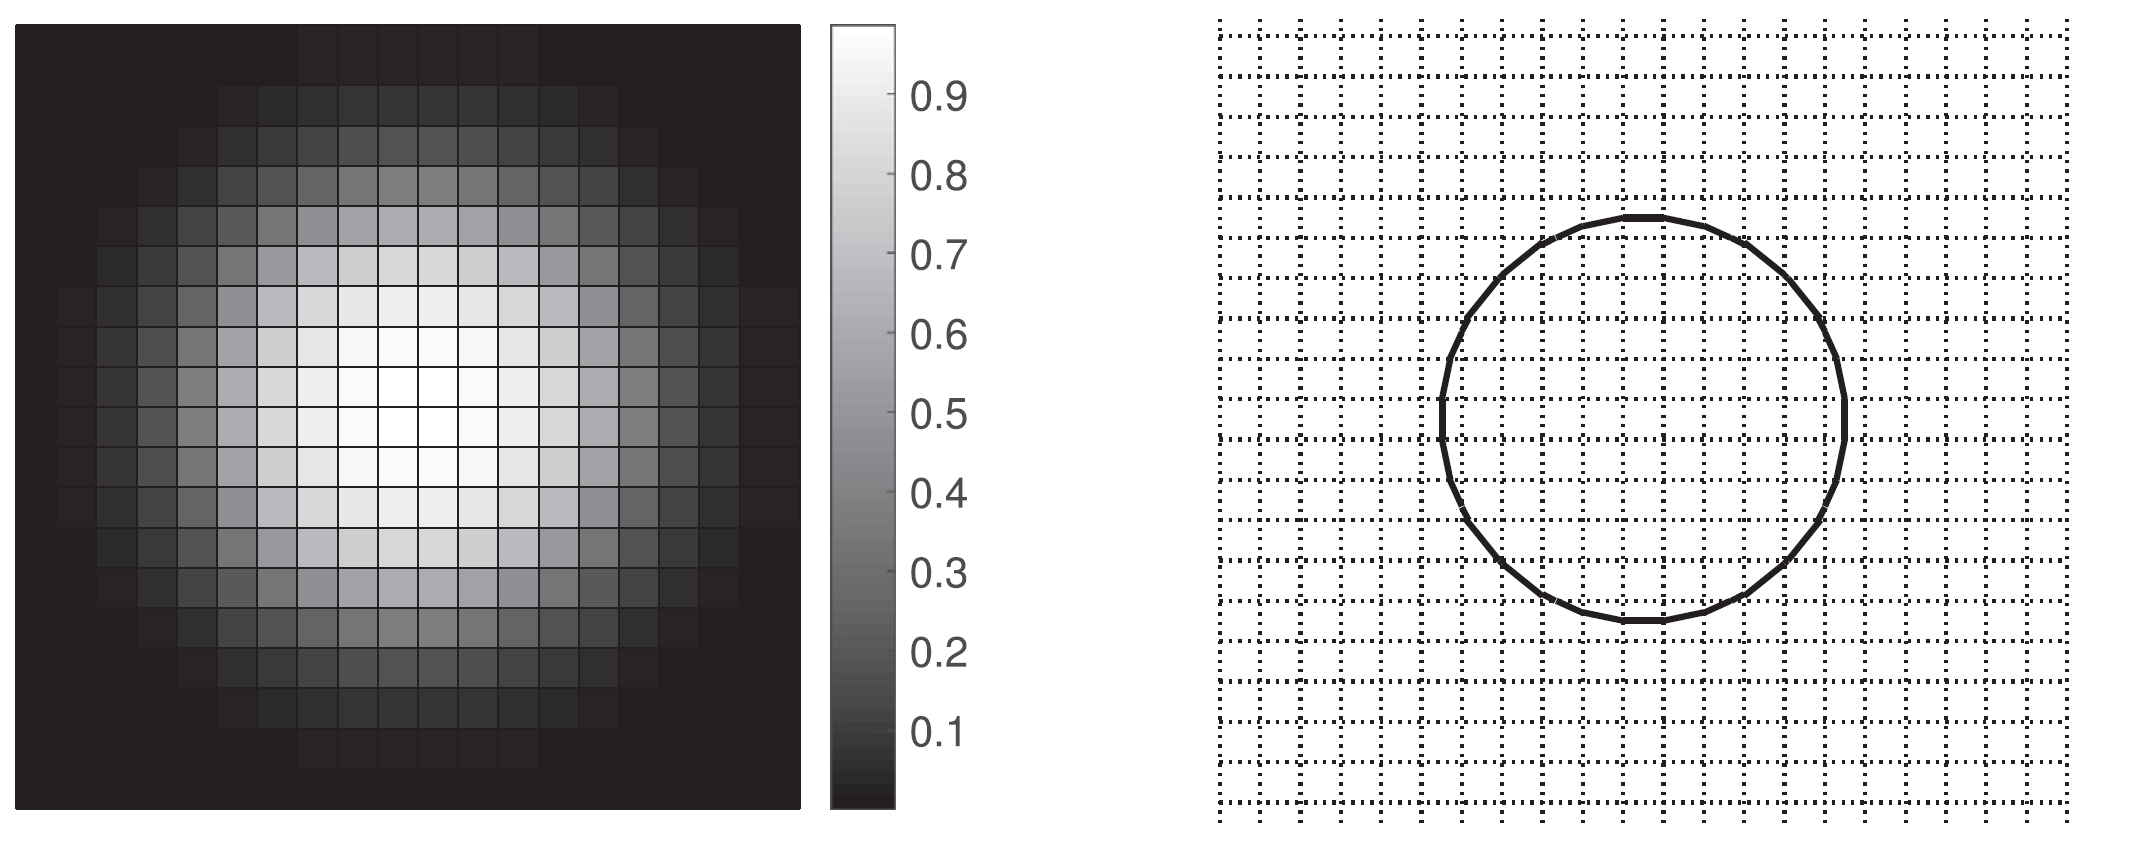
\includegraphics[scale=0.35]{./part1_numerical_approaches/figures_ch2/DI_vs_VOF_Mirjalili}
	\caption{Comparison of a droplet solved in a 20x20 grid by a diffuse interface method (\textit{left}) and a sharp-interface VOF method (\textit{right}). Source: \citeColor[mirjalili_comparison_2019]}
	\label{fig:DI_vs_VOF}
\end{figure}


A class of diffuse-interface methods arousing recent interest in immiscible, incompressible two-phase flows are the phase field methods. Originally, they make use of the Cahn-Hilliard equations \citepColor[cahn_free_1958]. Their derivation is based on the minimisation of a free energy functional, which leads to a typical convection-diffusion equation with source terms. This equation presents the main disadvantage that it is written in a non-conservative form, and hence it is not suitable for its application in immiscible flows \citepColor[mirjalili_conservative_2020]. This issue was later solved by \citeColor[chiu_conservative_2011], who claimed that the following second order equation can be used with the same purpose and applied to immiscible flows:

\begin{equation}
\frac{\partial \psi}{\partial t} + \nabla \left( \textbf{u}  \psi \right) = \nabla \left[ \gamma \left( \epsilon \nabla \psi - \psi \left( 1 - \psi \right) \frac{\nabla \psi}{| \nabla \psi |} \right) \right]
\end{equation}

where $\epsilon$ is a parameter defining the thickness of the interface, $\gamma = \max \left( \textbf{u} \right)$  and $\psi$ is a hyperbolic tangent function representing the distance from the interface, defined later in Eq. (\ref{eq:ACLS_psi_definition}). This equation is transported to obtain the evolution of the interface with time. Then, the velocity fields are obtained from the traditional Navier-Stokes equations with a one-fluid formulation, Eq. (\ref{eq:momentum_conservation_general_differential}). The density and viscosities are evaluated with the field function $\psi$:

\begin{subequations}
\begin{align}
\rho &= \psi \rho_l - \left( 1 -  \psi \right) \rho_g  \\
\mu &= \psi \mu_l   - \left( 1 -  \psi \right) \mu_l
\end{align}
\end{subequations}

Other available diffuse-interface methods have made use of the aforementioned Cahn-Hilliard and applied it to miscible flows \citepColor[teigen_diffuse-interface_2011] and to compressible two-phase systems \citepColor[shukla_interface_2010]. Furthermore, diffuse-interface methods find good applicability in particular thermodynamic regimes, such as multicomponent systems at supercritical conditions where surface tension is non-existent and a proper interface is not present \citemColor[dahms_transition_2013,jofre_transcritical_2021]. 




\subsection{Front-tracking method}

The front-tracking method is, according to the classification of Figure \ref{fig:classification_numerical_methods_mirjalili}, the only method presented in this chapter following an interface-tracking approach (the rest are comprised within the interface-capturing family). It was introduced for the first time by \citeColor[tryggvason_front-tracking_2001]. The interface is modeled as a moving front of lagrangian particles without mass which are explicitly tracked by connected marker points. Particles are convected with the flow field, and their movement is governed according to the kinematic equation:

\begin{equation}
\textbf{u} = \frac{d \textbf{x}}{d t}
\end{equation}

where the velocity $\textbf{u}$ is obtained by solving the flow field. As lagrangian particles are used, the interface is not solved in the same grid as the liquid and gas fields, see Fig. \ref{front_tracking_tryggvason}. This makes this method more of a lagrangian nature than an eulerian one in the sense that the interface is resolved separately from the main grid. Yet, both phases are solved with an eulerian formalisms within the same grid, making this method eulerian since it aims mainly at solving  separate-phase problems as indicated in Fig. \ref{fig:TPF_droplets_example} left. There are indeed interface-tracking methods dealing with the interface from an eulerian perspective, such as the Marker and Cell (MAC) method \citepColor[mckee_mac_2008].

\begin{figure}[h!]
	\centering
	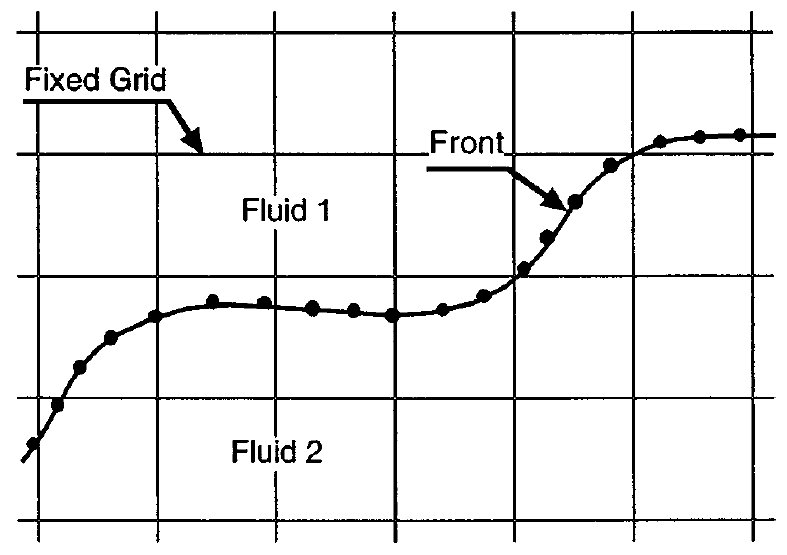
\includegraphics[scale=0.5]{./part1_numerical_approaches/figures_ch2/front-tracking_triggvason}
	\caption{Illustration of the front-tracking method: both fluids are solved in the main grid while the interface is represented by a front of particles. Source: \citeColor[tryggvason_front-tracking_2001]}
	\label{fig:front_tracking_tryggvason}
\end{figure}



\subsection{Volume of Fluid method}
\label{subsec:ch2_VOF}

% VOF reference: 2C. Hirth and B. Nichols. “Volume of Fluid (VOF) method for the dynamics of free boundaries”. In: Journal of Computational Physics 39 (1979), pp. 201–225

The Volume of Fluid method (VOF) is the first numerical methodologies developed to solve for liquid-gas interfaces in free surface flows, introduced originally by \citeColor[hirt_volume_1981]. It is included among the methods using a \textbf{sharp-interface} approach, as opposed to diffuse interface which were succinctly discussed in the previous section. They have been extensively studied in literature , and have been applied for both structured \citemColor[scardovelli_direct_1999,fuster_simulation_2009] and unstructured \citemColor[jofre_3-d_2014,ivey_conservative_2017] grids. VOF methods identify the liquid regions according to their liquid volume fraction $\alpha_l$ defined in Eq.(\ref{eq:volume_fraction_definition}). The volume fraction scalar is transported with an advection equation:

\begin{equation}
	\label{eq:VOF_alpha_advection}
	\frac{\partial \alpha_l}{\partial t} + \nabla \cdot \left( \alpha_l \boldsymbol{u} \right) = 0
\end{equation}

The material properties, density $\rho$ and viscosity $\mu$, are calculated from the liquid volume fraction:

\begin{subequations}
\begin{align}
\rho = \alpha_l \rho_l + \left( 1 - \alpha_l \right) \rho_g  \\
\mu = \alpha_l \rho_l + \left( 1 - \alpha_l \right) \rho_g
\end{align}
\end{subequations}


The biggest advantage of VOF is the mass conservation, as it is ensured when solving \ref{eq:VOF_alpha_advection}. On the other side, its main challenge if the difficulty of reconstructing the interface from the transported $\alpha_\mathrm{l}$ field, as illustrated in Figure \ref{fig:VOF_illustration_drawback}. According to the approach used to reconstruct the interface, VOF methods can be classified as algebraic or geometric \citemColor[mirjalili_interface-capturing_2017,pirozzoli_algebraic_2019].


\begin{figure}[h!]
	\centering
	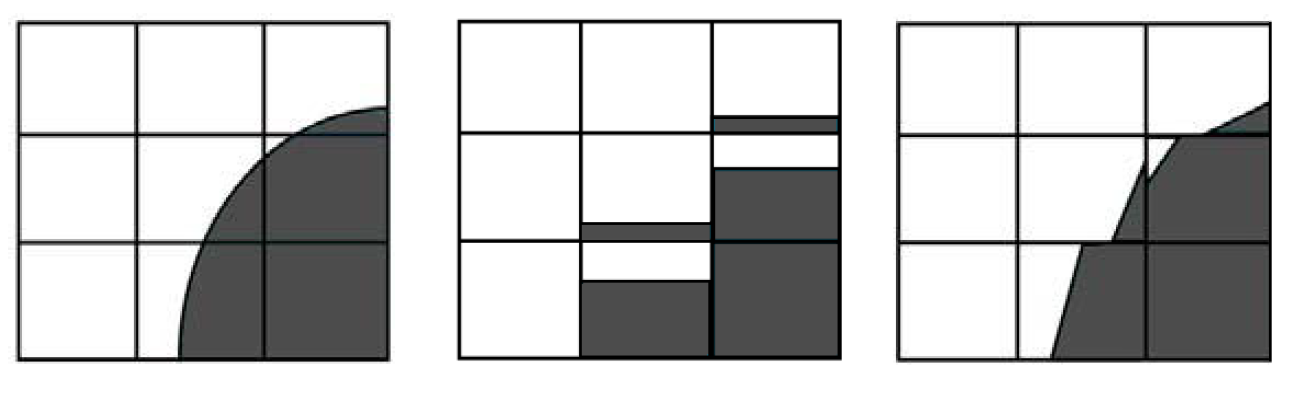
\includegraphics[scale=0.5]{./part1_numerical_approaches/figures_ch2/VOF}
	\caption{Application of VOF method, where dark is liquid and white is gas. \textsl{Left}: original $\alpha_\mathrm{l}$ field. \textsl{Middle}: transported $\alpha_\mathrm{l}$ field. \textsl{Right}: interface reconstruction, where a non-smooth interface can be appreciated. Source: \citeColor[odier_simulation_2006]}
	\label{fig:VOF_illustration_drawback}
\end{figure}


\subsection{Accurate Conservative Level Set method}
\label{subsec:ch2_ACLS}

% Osher and Fedkiw: https://link.springer.com/book/10.1007/b98879
% sussman: https://www.sciencedirect.com/science/article/pii/S0021999184711557
% Olsson articles:
%   https://www.ljll.math.upmc.fr/~hecht/ftp/Mireille-Haddad/A%20conservative%20level%20set%20method%20for%20two%20phase%20flow__Olsson_Kreiss.pdf
%   https://www.ljll.math.upmc.fr/~hecht/ftp/Mireille-Haddad/A%20conservative%20level%20set%20method%20for%20two%20phase%20flow%20II__Olsson.pdf


A well-known class of interface-capturing approaches for two-phase flows are the level set methods. As their own name indicates, these methods identify the interface as a constant value of a scalar level set function. The interface is directly represented and transported using this function, hence its location is always known and no reconstruction needs to be done (as opposed to VOF methods).

Classical level set methods \citepColor[osher_level_2003] distinguish between liquid and gaseous phases by introducing the smooth, signed-distance function to the interface $\phi(\textbf{x},t)$ :

\begin{equation}
\phi \left( \textbf{x},t \right)=\pm |\textbf{x}\left( t \right)-\textbf{x}_{\scriptsize{\Gamma}} \left( t \right)|
\end{equation}

According to this definition, the interface is located at $\phi(\textbf{x},t) = 0$. Positive values of $\phi(\textbf{x},t)$ indicate liquid regions, while negative values denote gas. The interface is then transported with an advection equation:

\begin{equation}
	\label{eq:LS_classical_advection}
	\frac{\partial \phi}{\partial t} + \nabla \cdot \left( \phi \boldsymbol{u} \right) = 0
\end{equation}

When applying the previous expression, the function $\phi$ will be distorted and its smoothness will be lost. To solvent this, the profile of $\phi$ is reshaped using a reinitialization equation \citepColor[sussman_level_1994] However, mass conservation is not ensured after the reinitialization process due to the nature of the distance function $\phi$. In this sense, \citeColor[olsson_conservative_2005] tried to reduce the conservation errors by introducing the hyperbolic tangent function $\psi$:

\begin{equation}
\label{eq:ACLS_psi_definition}
\psi \left( \textbf{x},t \right)=\frac{1}{2} \left(\tanh\left(\frac{\phi(\textbf{x},t)}{2\varepsilon}\right)+1\right)
\end{equation}

where $\varepsilon$ defines the interface thickness. The function $\psi$, which is a mapping from the classical signed-distance $\phi$, is bounded between $0$ and $1$, while $\phi$ is unbounded. The interface $\Gamma$ is located at the iso-value $\psi = 0.5$; gas phase is given by $\psi < 0.5$, and liquid for $\psi > 0.5$. Figure \ref{fig:psi_phi_profiles_janodet_2021_JCP} shows a representative view of both distance functions.

As in the classical level-set method, the hyperbolic tangent profile is also transported via an advection equation:

\begin{equation}
    \frac{\partial \psi}{\partial t} + \boldsymbol{\nabla} \cdot \left( \psi \textbf{u} \right) = 0
\end{equation}

and then reinitialised through resolution of the following equation \citepColor[olsson_conservative_2007]:


\begin{equation}
\label{eq:acls_reinit_2008}
\frac{\partial\psi}{\partial \tau}=\boldsymbol{\nabla}\cdot(\ \underbrace{\varepsilon(\boldsymbol{\nabla}\psi\cdot\textbf{n})\textbf{n}}_{\mathrm{Diffusion}}-\underbrace{\psi(1-\psi)\textbf{n}}_{\mathrm{Resharpening}})
\end{equation}

where $\tau$ is a pseudo-time and $\textbf{n}$ is the normal vector to the interface, obtained from the signed-distance function $\psi$:

\begin{equation}
\textbf{n} = \frac{\nabla \psi}{| \nabla \psi |} 
\end{equation}


As indicated in Eq. (\ref{eq:acls_reinit_2008}), the reinitialization process has two terms: diffusion and resharpening. Both of them are necessary to ensure the smoothness of $\psi$. With the introduction of $\psi$ and the reinitialization equation, mass conservation errors are reduced: hence, this method is referred as conservative level set. Nevertheless, numerical errors might appear during reinitialisation since small oscillations in $\psi$ might induce big variations in $\textbf{n}$. To improve the accuracy, \citeColor[desjardins_accurate_2008] proposed an extension to this conservative methodology in which the interface transport is solved with high order schemes and a fast-marching method is used to reconstruct the signed-distance function $\phi$. This function is then used to compute the interface normals and, with it, the curvature $\kappa$: 

\begin{equation}
\textbf{n} = \frac{\nabla \phi}{| \nabla \phi |} 
\end{equation}

\begin{equation}
\kappa = - \nabla \cdot \textbf{n}
\end{equation}

\citeColor[desjardins_accurate_2008] use a least squares reconstruction to compute $\kappa$. This extension to the conservative level set methodology is known as \textbf{Accurate Conservative Level Set} (ACLS) method. With these formulations, mass conservation is improved and numerical errors are reduced. ACLS is coupled to the Ghost-Fluid Method (GFM) \citepColor[fedkiw_non-oscillatory_1999] in order to deal explicitly with the pressure jump at the interface:

\begin{equation}
    \left[ p \right]_{\scriptsize{\Gamma}} = p_{l,{\scriptsize{\Gamma}}} - p_{g,{\scriptsize{\Gamma}}}  = \sigma \kappa_{\scriptsize{\Gamma}} + 2 \left[ \mu \right]_{\scriptsize{\Gamma}} \textbf{n}^T \cdot \nabla \textbf{u} \cdot \textbf{n}
\end{equation}

where $\kappa_\Gamma$ is the interface mean curvature and $\mu$ is the dynamic viscosity. Using this formulation, surface tension forces $\sigma\kappa_\Gamma$ are embedded in the pressure jump. \\

\begin{figure}[ht]
    \centering
    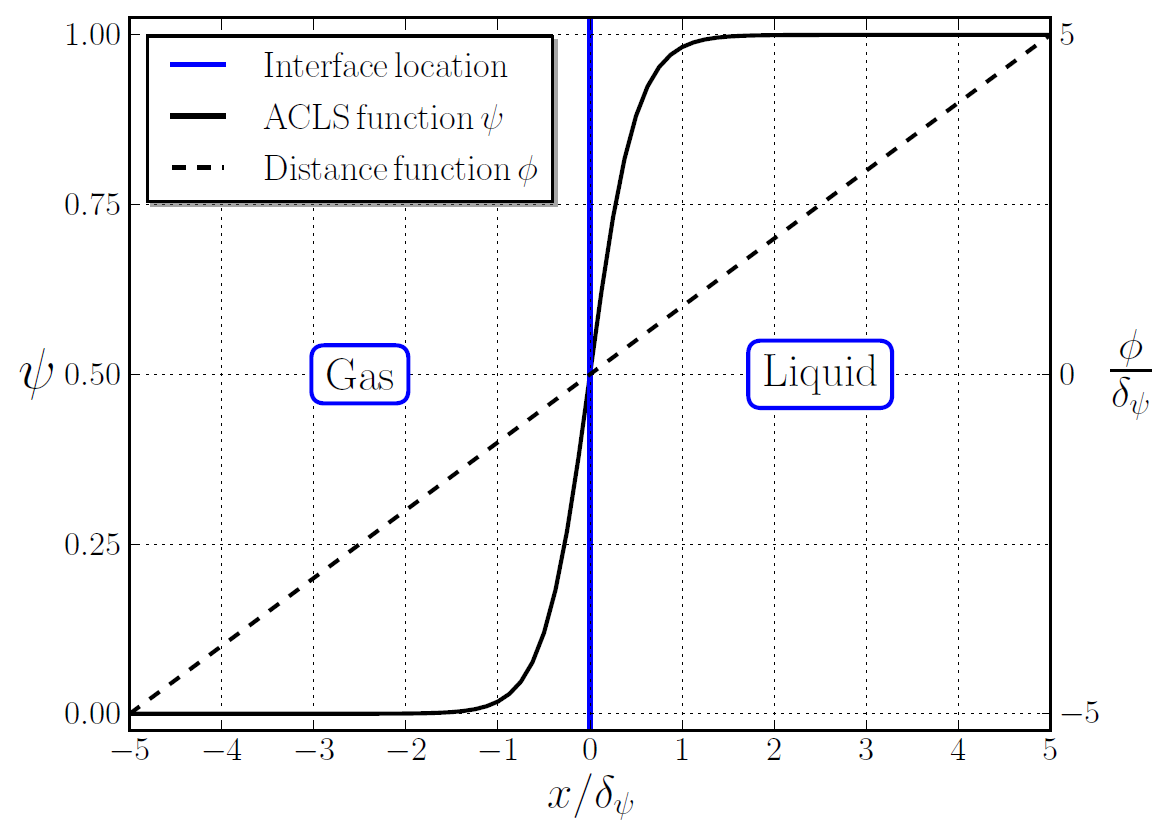
\includegraphics[width=0.6\textwidth]{./part1_numerical_approaches/figures_ch2/ACLS_psi_phi_janodet_JCP}
       \centering
    \caption{Representation of distance functions $\phi$ and $\psi$. The signed-distance function $\phi$ has been normalized by $\delta_\psi = 4\varepsilon$ for visualization. Source: \textbf{ref:Janodet-2021-JCP}.}
    \label{fig:psi_phi_profiles_janodet_2021_JCP}
\end{figure}



In this work, the more recent extension to the ACLS method by \textbf{ref:Janodet-2021-JCP} is used. This formulation makes use of the reinitialization equation introduced by \citeColor[chiodi_reformulation_2017]:

\begin{equation}
\label{eq:acls_reinit_2017}
\frac{\partial\psi}{\partial \tau}=\boldsymbol{\nabla}\cdot\left(\frac{1}{4\cosh^2{\left(\phi_{\mathrm{map}}/2\varepsilon\right)}}\left(|\boldsymbol{\nabla}\phi_{\mathrm{map}}\cdot\textbf{n}|-1\right)\textbf{n}\right)
\end{equation}

where $\phi_{\mathrm{map}}=\varepsilon\ln\left({\psi}/({1-\psi})\right)$ is an analytical signed-distance function mapped for $\psi \in ]0;1[$. This reinitialization equation ensures that the hyperbolic tangent profile $\psi$ is reshaped after transport without introducing significant spurious displacement of the interface. The curvature is then calculated as follows:

\begin{equation}
\kappa=\frac{\mathrm{Tr}\left(\boldsymbol{\mathcal{H}}(\phi)\right)-\frac{\boldsymbol{\nabla}\phi^T}{|\boldsymbol{\nabla}\phi|}\cdot\boldsymbol{\mathcal{H}}\left(\phi\right)\cdot\frac{\boldsymbol{\nabla}\phi}{|\boldsymbol{\nabla}\phi|}}{|\boldsymbol{\nabla}\phi|}
\label{eq:curvature_Goldman}
\end{equation}

where $\mathcal{H} \left( \phi \right)$ is the Hessian matrix of the distance function. To reduce numerical errors, a Geometric-Projection Marker Method (GPMM) is used reconstruct $\phi$ at the nodes in a narrow band around the interface \citepColor[janodet_unstructured_2019]. The GFM method is also used to deal with the interface pressure jump. Both phases are solved with a one-fluid formulation by solving Navier-Stokes and evaluating the physical properties at each spatial location with:

\begin{subequations}
\begin{align}
\rho(\textbf{x},t) &= \rho_g+(\rho_l-\rho_g)H(\psi(\textbf{x},t)-1/2)  \\
\mu(\textbf{x},t) &= \mu_g+(\mu_l-\mu_g)\psi(\textbf{x},t)
\end{align}
\end{subequations}



where $H$ is the Heaviside function.






\subsubsection*{Coupling with dynamic mesh adaptation}

To better resolve the atomization dynamics and save computational resources, the ACLS/GFM method is coupled to an Adaptive Mesh Refinement (AMR) strategy for increasing the mesh resolution at the liquid-gas interface at an affordable cost \citepColor[leparoux_primary_2018]. In AMR, the target element size at the interface $\Delta x_\mathrm{min}$ and  the number of cells with this size $N_p$ are specified by the user. The spatial region containing elements with size $\Delta x_\mathrm{min}$ has a width $2 N_p\Delta x_\mathrm{min}$, see Figure \ref{fig:AMR_strategy}. The mesh is dynamically refined throughout the computation with an automatic distance-based triggering ensuring that the interface always remains within this region. In its vicinity, the cell size increases linearly with controlled slope until the baseline cell size $\Delta x_\mathrm{init}$. AMR will be used in all the resolved atomization simulations presented in this thesis. Hence, the full methodology used to performed this simulations will be referred from now on as ACLS/AMR.

\begin{figure}[ht]
    \centering
    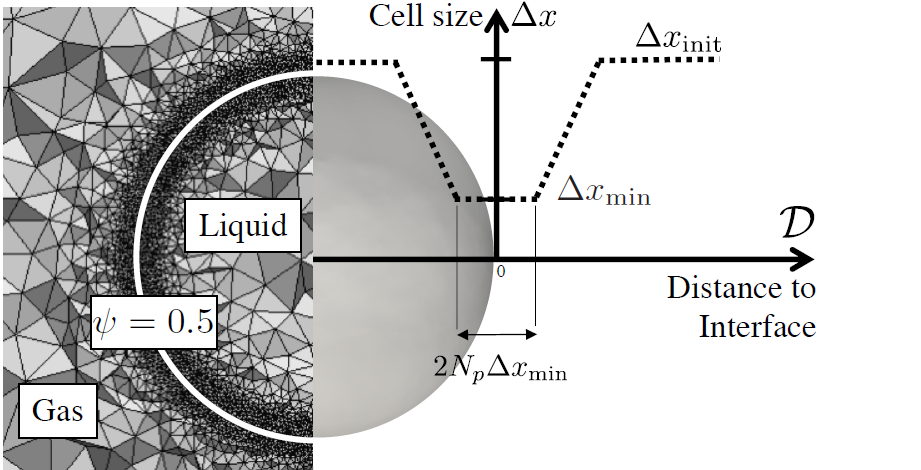
\includegraphics[width=0.6\textwidth]{./part1_numerical_approaches/figures_ch2/AMR}
       \centering
    \caption{Illustration of dynamic mesh adaptation with Adaptive Mesh Refinement. Source: \citepColor[leparoux_primary_2018].}
    \label{fig:AMR_strategy}
\end{figure}



\newpage

\chapter{Numerical methods to simulate dispersed phase}
	\label{ch3:disperse_phase_methods}

\section{Introduction}

The previous chapter presented numerical methodologies applicable to separate two-phase flows. These are useful for solving problems where the dynamics of atomization need to be accurately resolved. Nonetheless, those methods cannot be applied in the dispersed phase regime, where atomization is complete (or almost complete) and a spray composed of individual droplets is formed. Such problems, often found when studying reactive processes where fuel is injected into a combustion chamber, need a different representation of the liquid phase so that: 1) the spray can be transported with acceptable computational costs and 2) more complex physics relevant to reactive problems can be included, such as evaporation and combustion.

The spray generated in the dispersed phase regime is mainly distinguished from liquid in the separate regime by the following features (represented in Figure \ref{fig:atomization_regimes_herrmann}):

\begin{itemize}

	\item The characteristic length scales of the particles. In dispersed phase flows, these ones are low and usually smaller than the resolution of the main grid.
	
	\item The value of the liquid volume fraction $\alpha_l$. In dispersed phase flows, $\alpha_l < 1$. According its value, one can distinguish between dense regime (moderate values of $\alpha_l$, particles are close to each other) and dilute regime (lower values of $\alpha_l$, usually below $10^{-3}$, particles are far from each other).

\end{itemize}

The numerical formalisms to resolve dispersed phase flows will hence depend on these two characteristics. It is also important to consider the interaction with the gaseous phase, since its resolution depends of the main grid. The interaction between the liquid and gaseous phases in dispersed phase flows can be quantified by means of the Stokes number $St$, defined as the ratio between the characteristic time-scale of a liquid particle $\tau_p$ and a characteristic time of the gaseous phase $\tau_g$: 

\begin{equation}
\label{eq:Stokes_number_definition_general}
St = \frac{\tau_p}{\tau_g}
\end{equation}

A classification of numerical methods to simulate dispersed phase flows based on the volume fraction and the Stokes number has been done by \citeColor[balachandar_scaling_2009], shown in Figure \ref{fig:balachandar_numerical_methods_representation}. As it can be seen, the Stokes number will depend on the numerical methodology used to resolve the gaseous phase: in DNS, the smallest scales of turbulence with characteristic size $\upeta$ will be resolved and will have a characteristic time $\tau_k$, while in LES the smallest scales resolved $\upxi$ will be larger and their time-scales will be different ($\tau_\upxi$). Regarding the volume fraction, coupling strategies between liquid particles and gas can be used depending on its value: in the dilute regime particles are far from each other and the interactions among them can be neglected (one and two-way coupling), while in the dense regime the interaction between particles must be taken into account (four-way coupling). The difference between one and two-way coupling depends on if the influence of the liquid phase onto the gas is considered with source terms (two-way coupling) or if it is neglected, so that the gaseous phase will not be perturbed by the particles (one-way coupling).


\begin{figure}[h!]
	\centering
	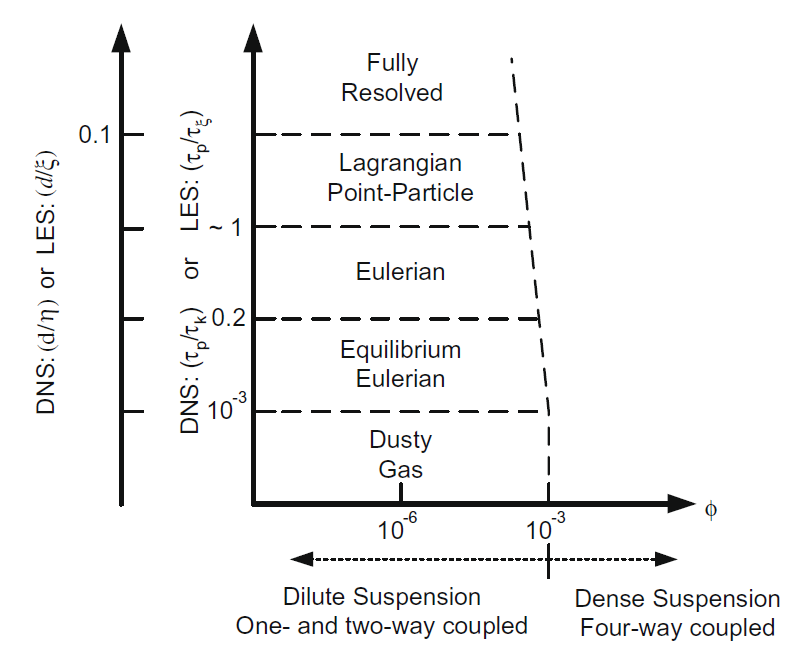
\includegraphics[scale=0.6]{./part1_numerical_approaches/figures_ch3/balachandar_disperse_phase_classification}
	\caption[Numerical approaches to solve dispersed phase flows]{Numerical approaches to solve dispersed phase flows. Classification is done with respect to the liquid volume fraction (here defined as $\phi$) and to the Stokes number or, equivalently, to the ratio of largest to smallest length scales, which depend on the numerical resolution.  Source: \citeColor[balachandar_scaling_2009]}
	\label{fig:balachandar_numerical_methods_representation}
\end{figure}

In this chapter, numerical strategies to simulate dispersed phase flows are reviewed. Section \ref{sec:ch3_numerical_approaches_dispersed_phase} summarizes some of the available formalisms that can be chosen for solving a dispersed phase problem, with special emphasis on the lagrangian point-particle approach which is employed in this thesis. Then, section \ref{sec:ch3_state_art_lagrangian_injection} presents the state of the art on lagrangian methods to simulate fuel injection in MSFI systems, which is the starting point of the works presented in this thesis.

\section{Numerical approaches to model dispersed phase flows}
\label{sec:ch3_numerical_approaches_dispersed_phase}


%The different dispersed phase methodologies aim at resolving Eq. (\ref{eq:WBE_spray_representation}), either by approximating this equation to obtain the function $f$ or by making point-particles assumptions, as shown in Figure \ref{fig:balachandar_numerical_methods_representation}. This chapter makes a review of some of these strategies, with special emphasis on the lagrangian point-particle approach which is employed in this thesis.

\subsection{Statistical methods}
\label{subsec:ch3_statistical_methods}

A spray composed of dispersed droplets can be characterized by means of a number density function $f$. This function depends on time $t$, space $\textbf{x}$, velocity $\textbf{u}$ and radius $r$, and can be expressed as follows \citepColor[subramanian_statistical_2000]:

\begin{equation}
\label{eq:f_spray_description_subramanian}
f \left( t, \textbf{x}, \textbf{u}, r \right) = \sum_{p=1}^{N_d} \delta \left( \textbf{x} - \textbf{x}_p \left( t \right) \right)  \delta \left( \textbf{u} - \textbf{u}_p \left( t \right) \right) \delta \left( \textbf{r} - \textbf{r}_p \left( t \right) \right)
\end{equation}

where $N_d$ is the number of droplets in the spray, and $\textbf{x}_p$, $\textbf{u}_p$ and $r_p$ are each individual particles position, velocity and radius respectively. The function $f$ contains all the necessary information to represent the spray. This function is governed by a William-Boltzmann Equation \citepColor[williams_spray_1958]:

\begin{equation}
\label{eq:WBE_spray_representation}
\frac{\partial f}{\partial t} + \nabla_{\textbf{x}_p} \left( \textbf{u}_p f \right) + \nabla_{\textbf{u}_p} \left( \textbf{F}_p f \right) + \frac{\partial E_{S_p} f}{\partial S_p} + \frac{\partial E_{T_p} f}{\partial T_p}
\end{equation}

where $\textbf{x}_p$, $\textbf{u}_p$, $S_p$ and $T_p$ are each individual particle's position, velocity, surface and temperature, respectively; $\textbf{F}_p$ is the force acting on the particle, and $E_S$ and $E_T$ are respectively the exchange terms due to mass (evaporation rate) and energy (heat transfer). Statistical approaches aim at determining the function $f$ by solving/approximating Eq. (\ref{eq:WBE_spray_representation}). Stochastic methods to solve for the dispersed phase include the stochastic lagrangian approach of \citeColor[dukowicz_particle-fluid_1980], eulerian methods considering a monodisperse \citepColor[drew_theory_1999] or a polydisperse spray \citepColor[laurent_multi-fluid_2001], and quadrature methods. These methods are out of the scope of the present work and hence are not discussed here.



\subsection{Eulerian methods}

Eulerian methods, also called Euler-Euler formalism (EE), are widely used to model dispersed two-phase flows. The same grid is used for resolving both the carrier and dispersed phases. The carrier phase is solved from the Navier-Stokes equations ($\S$\ref{sec:ch2_governing_equations}) applied to the gas. For characterizing the dispersed phase, averaged properties and statistical tools are used. These methods present, however, difficulties when dealing with the polydispersion of the spray and when modeling the particles collisions and interactions with the walls \citepColor[garcia_developpement_2009].

To solve for the dispersed phase, a well-known eulerian formalism is the mesoscopic approach. The particles are described according to the kinetic theory of gases formulated by \citeColor[chapman_mathematical_1970], so that mesoscopic variables are used to get averaged properties of the spray. In order to develop the equations for the dispersed phase, several assumptions need to be made \citepColor[lancien_etude_2018]:

\begin{enumerate}

\item The atomization process is complete, particles are perfectly spherical and non-deformable.

\item The only force exerted by the carrier phase on the droplets is drag.

\item Temperature is homogeneous inside each droplet.

\item Spray is dilute: $\alpha_l < 10^{-2}$.

\item The interactions between droplets are neglected.

\item The spray is mono-disperse and mono-kinetic: at one point in time and space, the droplets all have the same diameter and velocity.

\item Similarly, at one point in time and space, all droplets have the same temperature.

%\item Random uncorrelated motion is neglected.

\end{enumerate}

With these assumptions, the dispersed phase is represented by the following equations based on statistical averages of the spray \citepColor[lancien_etude_2018]:

\begin{subequations}
\label{eq:EE_disperse_phase}
\begin{align}
\frac{\partial \overline{n}_l}{\partial t} + \nabla \left( \overline{n}_l \overline{\textbf{u}}_l \right)  &= 0 \\
\frac{\partial \rho_l \overline{\alpha}_l}{\partial t} + \nabla \left( \rho_l \overline{\alpha}_l \overline{\textbf{u}}_l \right) &= - \Gamma \\
\frac{\partial \rho_l \overline{\alpha}_l \overline{u}_{l,i}}{\partial t} + \nabla \left( \rho_l \overline{\alpha}_l \overline{\textbf{u}}_l \overline{u}_{l,i} \right) &= F_{d,i} - \overline{u}_{l,i} \Gamma  + \nabla \overline{\overline{\pmb{\tau}}}_l^{sgs} \\
\frac{\partial \rho_l \overline{\alpha}_l \overline{h}_l}{\partial t} + \nabla \left( \rho_l \overline{\alpha}_l \overline{\textbf{u}}_l  \overline{h}_l \right) &=  - \overline{h}_l  \Gamma + \overline{\Phi}
\end{align}
\end{subequations}

where $n_l$ is the number density of the particles, $\Gamma$ the evaporation rate, $F_{d}$ the drag force, $\overline{\overline{\pmb{\tau}}}_l^{sgs}$ the subgrid tensor of the liquid phase, $\overline{h}_l$ the liquid enthalpy and $\overline{\Phi}$ the conduction flux term. The exchange between phases is taken into account by the right hand sides of the previous expressions. As it is observed, multiphysics phenomena such as mass exchange due to evaporation and energy transfer can be taken into account with the corresponding exchange terms.  This is one of the advantage of the dispersed phase modelling of two-phase flows as opposed to the fully-resolved atomization methods presented in Chapter \ref{ch2:numerical_methods_resolved_atomization}. 

\subsection{Lagrangian point particle representation}
\label{sec:ch3_EL_formalisms}

Another well-know methodology to simulate dispersed phases systems, broadly employed in aerospace applications, is the lagrangian point particle (LPP) representation. In this formalism, the gas is resolved in the main eulerian grid, but the particles conforming the dispersed phase are tracked individually and represented by a different set of equations. Since the carrier phase is solved in an eulerian grid and the dispersed phase is modeled separately, these method is usually referred as the Euler-Lagrange (EL) formalism. This can make convergence difficult and hinders the introduction of parallelism techniques. As advantages, the resulting the time per iteration is usually lower than for the EE description, and the drop-drop and drop-wall interactions are easier to model.

\subsubsection*{Dynamics of liquid particles}

For describing particles in the lagrangian framework, each particle will be modelled according to the \textbf{Discrete Particle Simulation} (DPS) approach. In DPS, liquid particles are completely spherical, robust, and defined spatially as points, so that the location of each parcel can be represented by a single position vector. With these assumptions, the \textbf{dynamic equations} for a particle $p$ are \citepColor[maxey_equation_1983]:

\begin{subequations}
\label{eq:TPF_lagrange_dynamic_eqs}
\begin{align}
\frac{d \boldsymbol{x}_p}{d t} &= \boldsymbol{u}_p \\
\frac{d \boldsymbol{u}_p}{d t} &= \underbrace{ - \frac{3}{4} \frac{\rho_\mathrm{g}}{\rho_p} \frac{C_D}{d_p} | \boldsymbol{v}_r | \boldsymbol{v}_r }_{\text{Drag}\atop\text{term}}  + \underbrace{ \left( 1 - \frac{\rho_\mathrm{g}}{\rho_p} \right) \boldsymbol{g} }_{\text{Gravity}\atop\text{term}} 
\end{align}
\end{subequations}

where $\textbf{x}_p$ and $\textbf{u}_p$ are the position and velocity of the particle, $\textbf{v}_r = \boldsymbol{u}_p  - \boldsymbol{u}_g$ the relative velocity between the particle and the gas, $\rho_\mathrm{g}$ and $\rho_p$ are the gas and liquid particle densities, $C_D$ a drag coefficient, and $d_p$ the particle diameter. Equation (\ref{eq:TPF_lagrange_dynamic_eqs}b) is the momentum equation of the droplet and contains the contributions of the two forces considered: the drag force and the gravitational forces. The former ones are usually the main mechanism of momentum transfer between phases, while the latter are often several orders of magnitude lower than the first ones and can often be neglected (specially at high speeds, where drag dominates the momentum transfer). 

The drag coefficient of the particles $C_d$ can be evaluated with the following expression, obtained experimentally by \citeColor[schiller_drag_1935]:

\begin{equation}
\label{eq:Re_CD_droplet}
C_D =
\left\{
    \begin{split}
     \frac{24}{Re} \left( 1 + 0.15 Re^{0.687} \right)\,\,\mathrm{if}\,\,Re < 1000 \\ 
    0.44\,\,\mathrm{if}\,\,Re \geq 1000 
    \end{split}
\right.
\end{equation}

where $Re = \rho_\mathrm{g} | \boldsymbol{v_r} | d_p / \mu_\mathrm{g} $ is the Reynolds number based on the relative velocity and particle diameter. \\

When considering a lagrangian approach, the influence of the carrier phase on the liquid particles will have a determining effect on their motion. This influence can be quantified by means of the Stokes number defined previously by Eq. (\ref{eq:Stokes_number_definition_general}). Its magnitude indicates how the droplet responds to fluctuations of the gas flow. If $St << 1$, the droplet will follow perfectly the fluctuations of the gas flow. On the contrary, if $St >> 1$ the droplets will rather neglect the flow trajectories and follow its own track (ballistic behaviour). 

For evaluating the Stokes number, the characteristic timescale for each phase need to be determined. The gaseous timescale can be determined as $\tau_g = d_p / | \textbf{u}_p |$. Particle timescales can be estimated from the following expression \citepColor[maxey_equation_1983]:

\begin{equation}
\tau_p = \frac{d_p^2 \rho_p}{18 \mu_\mathrm{g}} =  \frac{4}{3} \frac{\rho_p}{\rho_\mathrm{g}} \frac{d_p}{C_D | \boldsymbol{v}_r |} = \frac{4}{3} \frac{\rho_p d_{p^2}}{\mu_g Re C_D}
\end{equation}

which can be seen as the relaxation time of the particle; in other words, the time that one particle takes to respond to the fluctuations in the velocity field.


\subsubsection*{Coupling with mass and energy transfer}

As in the EE method, the LPP representation also allows to couple the dynamic equation with exchange terms for mass and energy transfer with the gaseous phase:

\begin{subequations}
\label{eq:TPF_lagrange_phasetransition_eqs}
\begin{align}
\frac{d m_p}{d t} &= \dot{m}_p = \Gamma \\
\frac{d h_p}{d t} &= m_p C_{P_\mathrm{g}} \frac{d T_p}{d t} = \Phi
\end{align}
\end{subequations}

where $m_p$, $h_p$, $T_p$ and $C_{P_\mathrm{g}}$ are respectively the particle mass, enthalpy, temperature and gas specific heat capacity at constant pressure. $\Gamma$ and $\Phi$ are the corresponding source terms for mass and energy. It follows that Equation (\ref{eq:TPF_lagrange_phasetransition_eqs}a) accounts for the \textbf{evaporation} process. If a single component is considered and the uniform temperature model for evaporation is used \citepColor[abramzon_droplet_1989], then the evaporation term can be expressed as:

\begin{equation}
\Gamma = - \pi d_p Sh \left( \rho_p D_F \right) \ln \left( 1 + B_M \right)
\end{equation}

where $Sh$ is the Sherwood number, $D_F$ the fuel diffusivity, and $B_M$ the Spalding mass number. \\

For evaluating the energy transfer in the droplets, the physical processes of \textbf{conduction} and  \textbf{evaporation} are taken into account. Then, the source $\Phi_p$ is obtained from the following energy balance.

\begin{equation}
\Phi_p = \underbrace{ h_p \pi d_p^2 \left( T_\mathrm{g} - T_p \right) }_{\text{Conduction}\atop\text{term}} - \underbrace{ \dot{m}_p  \Delta h_v }_{\text{Evaporation}\atop\text{term}}
\end{equation}

where $T_\mathrm{g}$ is the gas temperature, $h_p$ is the film coefficient of the gas at the particle surface and $\Delta h_v$ is the latent heat of vaporization of the particle. Eqs. (\ref{eq:TPF_lagrange_phasetransition_eqs}) can be solved together with Eqs. (\ref{eq:TPF_lagrange_dynamic_eqs}) to obtain the evolution of mass and energy of the droplets with time as they move within the carrier phase.

\section{Stage of the art in injection models for MSFI systems}
\label{sec:ch3_state_art_lagrangian_injection}

Several numerical formalisms for modeling the dispersed phase in two-phase flows have been introduced in the previous section. The choice of formalism will depend on the characteristics of the problem to solve. In this work, the lagrangian representation presented in $\S$\ref{sec:ch3_EL_formalisms} is used to model the dispersed phase due to its low computational cost and its applicability to account for polydispersity of the spray.%, which is of particular interest to develop realistic lagrangian injectors as stated in $\S$\ref{sec:ch1_objective_thesis_outline}.

In all dispersed-phase simulations, the first step is to introduce the lagrangian droplets in the domain with their proper boundary conditions. This is achieved by means of \textbf{lagrangian injection models}, which is the main interest of the present work. The fact of using a lagrangian approach for representing the particles has the advantage of allowing the injection of a polydisperse spray from the beginning of the simulation, something which is not possible with other dispersed formalisms such as the eulerian ones. This is of particular interest for performing injection in realistic systems, such as in MSFI configurations presented in $\S$\ref{sec:ch1_fuel_injection_technology}. 

This section presents the state of the art in models for lagrangian injection with particular focus on MSFI systems. Figure \ref{fig:state_art_injection} proposes a classification for existing models in literature grouped in a Venn diagram, distinguishing five categories and their interactions. Each research work is located according to the characteristics of the model employed, and the configuration of application within the MSFI models (hollow cone, airblast and JICF) is also specified. Several models are \textbf{based on empirical laws} obtained from experimental works, with the advantage that the physics of the problem are already embedded in these laws, but with the disadvantage that the application of these models is restricted to the geometry and operating conditions of the test. Regarding the size of injected droplets, it is found that the \textbf{injection of a fully developed spray} is usually performed, often obtained from experiments providing the spray granulometry further downstream the injection nozzle where atomization is fully complete. In the sense of droplet transport, it is sometimes necessary to consider the \textbf{effect of the dense spray in the gaseous phase}: in some configurations (specially in the JICF), coherent structures of the dense regime where primary atomization takes place might perturb the gaseous flow which will consequently affect the convection of droplets further downstream. Since the dense regime is neglected in lagrangian computations, this liquid-gas interaction is not taken directly taken into account, so the droplet transport might not be well resolved. In this respect, some methodologies have considered this interaction. Furthermore,  \textbf{secondary breakup of particles} in lagrangian simulations can be considered by means of secondary atomization models. This is specially useful in models which do not inject a developed spray, as the initial droplets will have a larger size than the diameters found in the equivalent real configuration. Independently of evaporation, the decrease of droplets size up to a value which is in equilibrium with the surrounding air can be accounted for with these models.

In the last place, a category called \textbf{reference spray learning} is present in Figure \ref{fig:state_art_injection}. It would include models that can use a reference spray to learn its characteristics (droplets sizes, velocity distributions and injection location) and impose realistic spray boundary conditions in dispersed phase simulations. As main advantage, such models could be applied to a wide range of injector configurations and operating conditions. Nevertheless, they require a proper characterization of the spray coming from simulations or experiments. This thesis aims at providing a numerical methodology for developing injection models that are able to follow this reference spray learning process. These models are explained in Chapter \ref{ch4:sli_development}, so they will not be further discussed in this section. The next lines are then devoted to explain some of the injection models in Figure \ref{fig:state_art_injection} which are of interest for MSFI systems, whose main mechanisms of injection are shown in Figure \ref{fig:multipoint_injector_snecma}.

%Each category has the following advantages and disadvantages (see presentation 2020 12 15):
%
%\begin{itemize}
%
%	\item \textbf{Based on empirical laws}. \textcolor{green}{Advantage}: embedded physics. \textcolor{red}{Disadvantage}: restricted to geometry and operating conditions of development.
%	
%	\item \textbf{Injection of fully developed spray}. \textcolor{green}{Advantage}: droplets size distributions directly imposed. \textcolor{red}{Disadvantage}: Primary atomization neglected.
%	
%	\item \textbf{Effect of dense spray in gaseous phase}. \textcolor{green}{Advantage}: in JICF, taking into account blockage effect. \textcolor{red}{Disadvantage}: None.
%	
%	\item \textbf{Addition of secondary atomization model}. Good if atomziation not present.
%	
%	\item \textbf{Reference spray learning}. So far, and to our knowledge, there are no available models that can use a reference spray to learn boundary conditions (droplet sizes, velocity distributions, spatial location of injectors) for dispersed phase computations. \textcolor{green}{Advantage}: Applicable to generic injectors and 
%	wide range of operating conditions.  \textcolor{red}{Disadvantage}: Need of detailed spray characterisation from simulations or experiments.
%
%\end{itemize}

%\begin{figure}[h!]
%	\centering
%	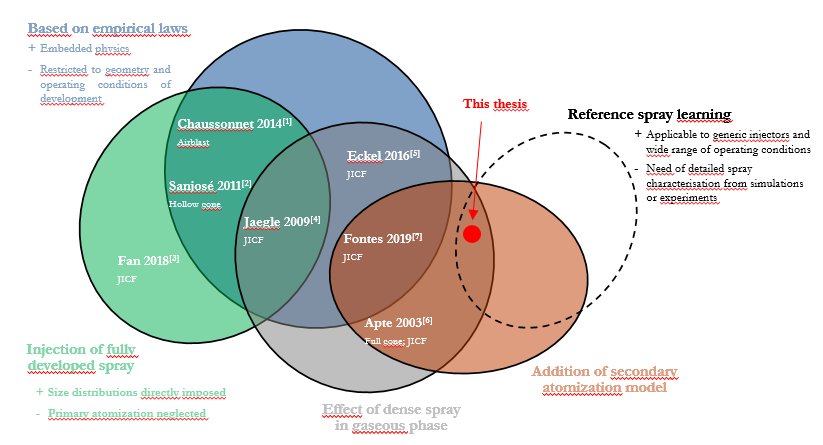
\includegraphics[scale=0.5]{./part1_numerical_approaches/figures_ch3/state_art_lagrangian}
%	\caption{Classification of lagrangian injection models}
%	\label{fig:state_art_injection}
%\end{figure}

\begin{figure}[h!]	
	\centering
	\includeinkscape[inkscapelatex=true,scale=0.75]{./part1_numerical_approaches/figures_ch3/state_art_lagrangian}
	\caption{Classification proposed for the state of the art in lagrangian injection modeling.}
	\label{fig:state_art_injection}
\end{figure}

\subsection{Hollow cone spray}
\label{subsec:ch3_hollow_cone_spray}

Pressure-swirl atomizers for delivering fuel through the pilot stage in multi-staged injectors will create a hollow cone spray. These type of nozzles are widely used and have been extensively studied both experimentally and numerically. Several models exist in literature for modeling the fuel injection in pressure-swirl with lagrangian formalisms. In this section two models are presented: the FIM-UR methodology developed by \citepColor[sanjose_fuel_2011], and the LISA model presented in \citeColor[guedot_developpement_2015].


\subsubsection*{FIM-UR model}

Fuel Injection Model by Upstream Reconstruction (FIM-UR) is an injection model which prescribes a developed spray in pressure-swirl atomizers, neglecting the atomization process. In its original formulation by \citeColor[sanjose_fuel_2011], a monodisperse spray is imposed. The extension to polydisperse sprays has been done by \citeColor[vie_accounting_2013].

The principles of FIM-UR are shown in Figure \ref{fig:FIMUR_methodology}. The spray is imposed at an injection location $x_i$, whose boundary conditions are obtained by reconstruction from the properties at the real injection location $x_0$. FIM-UR can be applied for both EL and EE simulations, with the difference that the latter require additional analytical calculations to determine the momentum transfer and the entrained air mass flow rate. Both cases use the same model inputs: the spray is characterized by the diameter of droplets $d$ and the half-spray mean angle $\theta_s$, and the atomizer is parametrized by its exit radius $R_0$ and the injected liquid mass flow rate $\dot{m}_l$. Then, empirical formulas for pressure-swirl atomizers are used to calculate the remaining parameters of the model. The ratio $X$ of the air core surface $A_a$ to the discharge orifice surface $A_o$, called the contraction ratio, is given by \citeColor[rizk_internal_1985]:

\begin{equation}
X = \frac{A_a}{A_0} = \left( \frac{R_a}{R_0} \right)^2 = \frac{\sin^2 \theta_s}{1 + \cos^2 \theta_s}
\end{equation}

From this formula, the air core radius $R_a$ can be solved. The contraction ratio $X$ can now be used to estimate the discharge coefficient of the atomizer \citepColor[lefebvre_atomization_2017]:

\begin{equation}
C_D = 1.17 \sqrt{\frac{\left( 1 - X \right)^3}{1 + X}}
\end{equation}

which can be used to obtain the tangential-injection surface $A_p$:

\begin{equation}
A_p = 20.73 C_D^2 A_0
\end{equation}

With all these parameters known the axial, radial and tangential velocities at the real injection location $x_0$ can be obtained:

\begin{subequations}
\label{eq:ch3_FIMUR_velocities_at_x0}
\begin{align}
u_x^0 \left( \theta, r_0 \right) &= \frac{\dot{m}_l}{\rho_l \pi \left( R_0^2 - R_a^2 \right)} \\
u_r^0 \left( \theta, r_0 \right) &= 0 \\
u_\theta^0 \left( \theta, r_0 \right) &= \frac{\dot{m}_l}{\rho_l A_p} \frac{r_0}{R_S^0} 
\end{align}
\end{subequations}

Finally, the properties at the numerical injection location $x_i$ are calculated by applying mass and momentum balances between $x_0$ and $x_i$ \citepColor[sanjose_fuel_2011]:

\begin{subequations}
\begin{align}
u_x^i \left( \theta, r_0 \right) &= \frac{\pi R_0^2}{\rho_l I_\alpha A_u} \exp \left( - \frac{\left( r - \mu \right)^2}{\sigma^2} \right) \\
u_r^i \left( \theta, r_0 \right) &= \frac{\dot{m}_l}{\rho_l A_p} \sqrt{1 - \left( \frac{R_S^0}{R_S^i}  \right)^2} \frac{r}{R_S^i} \\
u_\theta^i \left( \theta, r_0 \right) &= \frac{\dot{m}_l}{\rho_l A_p} \frac{R_S^0}{R_S^i} \frac{r}{R_S^i} 
\end{align}
\end{subequations}

where $\mu$, $\sigma$ are respectively the mean and variance of the gaussian profile of volume fraction at $x_i$ (see Figure \ref{fig:FIMUR_methodology}) and $I_\alpha = \sigma^2 \left( 1 - \exp \left( - R_i^2/\sigma^2 \right) \right) + \sigma R_S^i \sqrt{\pi} \erf \left( R_i / \sigma \right)$.


\begin{figure}[ht]
    \centering
    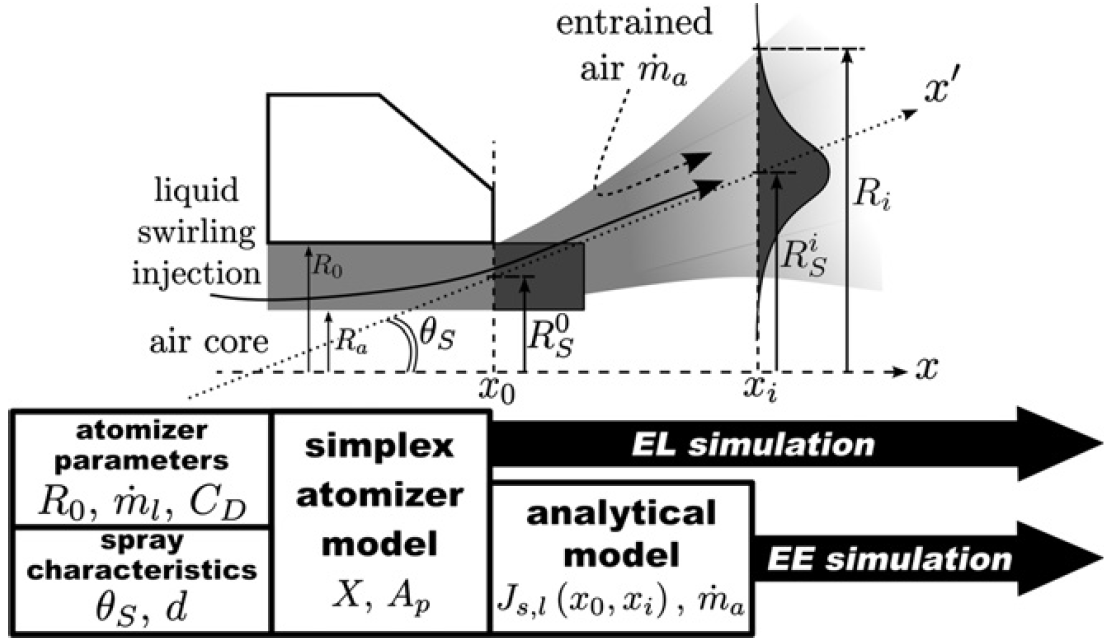
\includegraphics[width=0.7\textwidth]{./part1_numerical_approaches/figures_ch3/FIMUR}
       \centering
    \caption[FIMUR model for injection in pressure-swirl atomizers]{FIMUR model for injection in pressure-swirl atomizers. Source: \citeColor[sanjose_fuel_2011].}
    \label{fig:FIMUR_methodology}
\end{figure}

\newpage

\subsubsection*{LISA model}

The main disadvantage of the FIM-UR model is the inability to prescribe the mean angle $\theta_s$ in certain cases. To solvent this issue, \citeColor[guedot_developpement_2015] proposed the Liquid Injection for Swirled Atomizers (LISA) model. This methodology, described in Figure \ref{fig:LISA_methodology}, follows the same baseline as FIM-UR, but proposes some modifications to keep the mean spray angle constant.

The model inputs are the liquid mass flow rate $\dot{m}_l$, the spray mean angle $\theta_s$ and the atomizer exit radius $R_0$. The principles are identical to FIM-UR: droplets have no radial velocity at injection, and the axial velocity is obtained from mass conservation with the injected flow rate. Hence, both are calculated respectively with Equations (\ref{eq:ch3_FIMUR_velocities_at_x0}a) and (\ref{eq:ch3_FIMUR_velocities_at_x0}b). The tangential (or azimuthal) velocity imposed is calculated according to the derivations of \citeColor[guedot_developpement_2015]:

\begin{equation}
\label{eq:LISA_model_u_theta}
u_\theta \left( r \right) = u_z  \frac{r}{R_S^0} \tan \sigma_s
\end{equation}


\begin{figure}[ht]
    \centering
    \includeinkscape[inkscapelatex=true,scale=0.85]{./part1_numerical_approaches/figures_ch3/LISA_model}
    %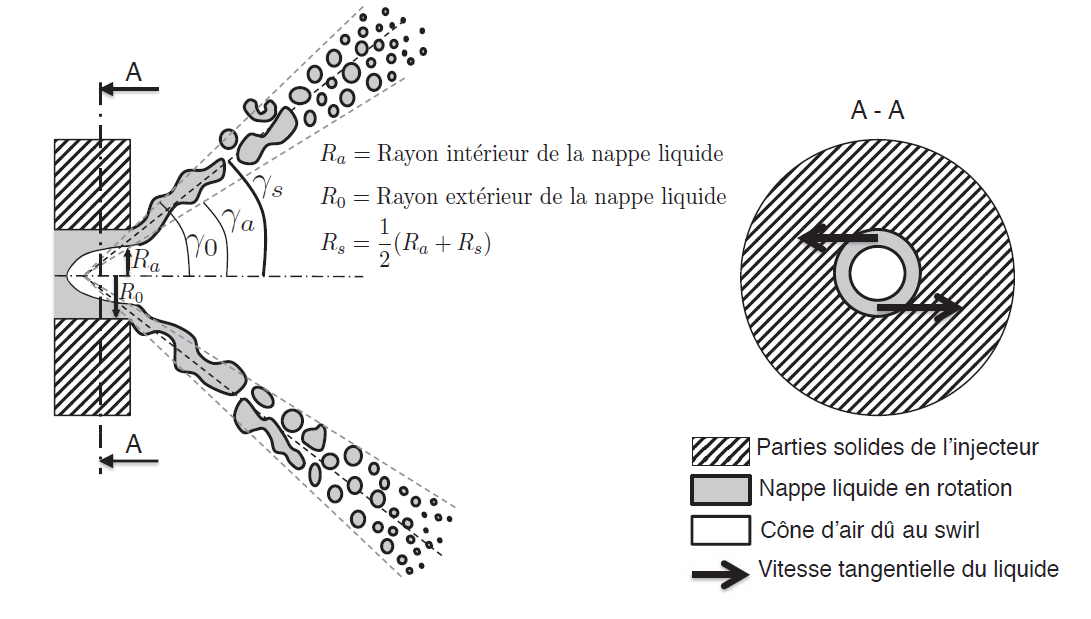
\includegraphics[width=0.8\textwidth]{./part1_numerical_approaches/figures_ch3/LISA}
       \centering
    \caption{LISA model for injection in pressure-swirl atomizers. Source: \citeColor[guedot_developpement_2015].}
    \label{fig:LISA_methodology}
\end{figure}



\subsection{Airblast spray}

In MSFI, at certain operating conditions the liquid injected through the pilot or take-off stages can impinge the walls of the atomizer forming an airblast spray, see Figure \ref{fig:multipoint_injector_snecma}. Airblast sprays have been extensively studied \citemColor[lefebvre_airblast_1980, gepperth_pre-filming_2010] and used in industrial burners, found in atomizers of type plain jet or prefilmers \citepColor[lefebvre_atomization_2017].

Regarding numerical approaches to simulate airblast sprays, a phenomenological model was derived by \citeColor[chaussonnet_new_2016] called PAMELA (Primary Atomization Model for prEfilming airbLAst injectors). This model uses results obtained in the KIT-ITS airblast experiment by \citeColor[gepperth_pre-filming_2010] for predicting initial conditions for droplets sizes and velocities. Correlations and laws for droplets sizes are derived by observing the breakup mechanisms found in airblast spray, shown in Figure \ref{fig:airblast_breakup_mechanism_chaussonnet}. This thesis does not address airblast atomization and hence the PAMELA model is no longer discussed here, the interested reader is referred to \citeColor[chaussonnet_modeling_2014] and \citeColor[chaussonnet_new_2016] for more details.

\begin{figure}[ht]
    \centering
    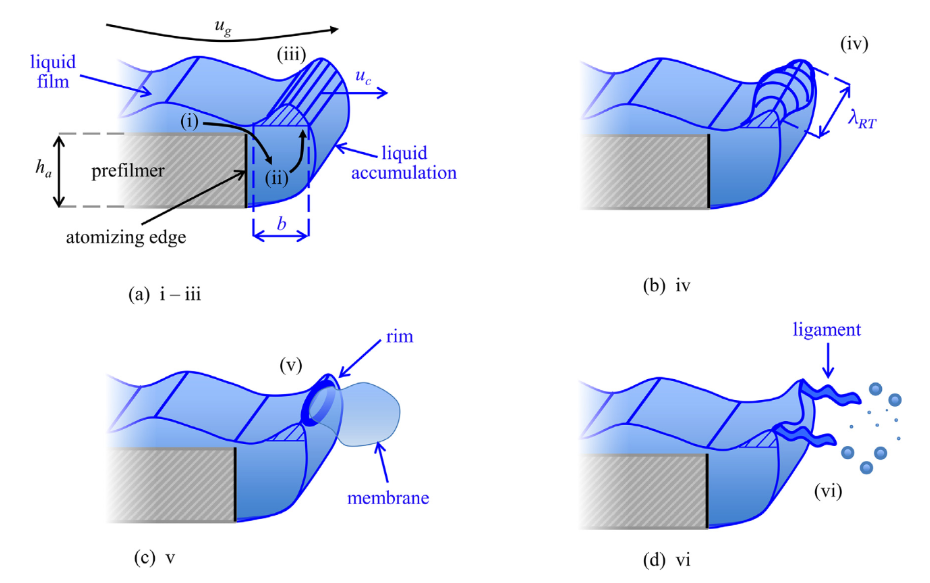
\includegraphics[width=0.8\textwidth]{./part1_numerical_approaches/figures_ch3/airblast_breakup_mechanism_chaussonnet}
       \centering
    \caption[Breakup mechanism in an airblast prefilmer spray]{Breakup mechanism in an airblast prefilmer spray. Source: \citeColor[chaussonnet_new_2016].}
    \label{fig:airblast_breakup_mechanism_chaussonnet}
\end{figure}




\subsection{Liquid jet in crossflow}
\label{ch3:subsec_lagrangian_liquid_JICF}

Several numerical approaches have been used to study liquid jet in crossflow injection, whose phenomenology has been introduced in $\S$\ref{sec:ch1_fuel_injection_technology}. Some works \citemColor[herrmann_detailed_2009,pai_role_2009,behzad_surface_2016,li_detailed_2018] have been devoted to resolved simulations of the atomization process, performed with the methodologies introduced in Chapter \ref{ch2:numerical_methods_resolved_atomization}. Such studies are useful to get insight on the dynamics and the underlying physical phenomena governing breakup, as well as to obtain information on the size and velocity distributions of droplets generated. However, these methods are computationally expensive and become unfeasible for simulating realistic gas turbines and coupling other physics such as evaporation and combustion. To solvent this issue, numerical models based on dispersed phase computations can be used. The rest of this chapter makes a review of such methodologies.

Figure \ref{fig:jaegle_jicf_modeling_approaches} shows four possible modeling approaches for performing simulations of liquid jet in crossflow. The approach (a) is the direct simulation of the jet (resolved atomization) mentioned in the last paragraph. The other three englobe several ways of tackling JICF simulations from a lagrangian perspective, where droplets are injected. All the categories from Figure \ref{fig:jaegle_jicf_modeling_approaches} take into account, one way or another, the liquid column (dense core) and hence its influence on the gaseous phase. The methods presented in this section are classified accordingly to the depicted lagrangian approaches, and are shown in chronological order.

\begin{figure}[ht]
    \centering
    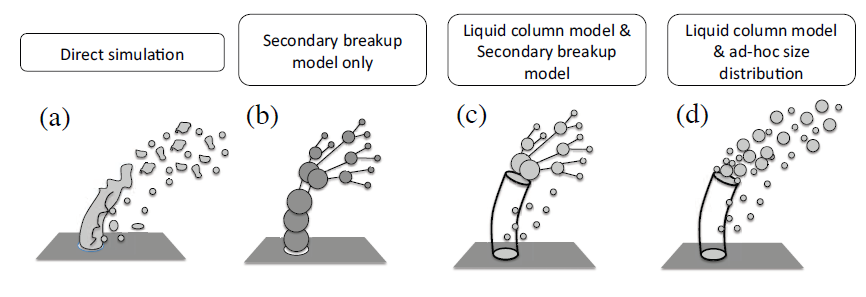
\includegraphics[width=1.0\textwidth]{./part1_numerical_approaches/figures_ch3/modelling_approaches_JICF_Jaegle}
       \centering
    \caption{Modeling approaches for liquid jet in crossflow proposed by \citeColor[jaegle_large_2009].}
    \label{fig:jaegle_jicf_modeling_approaches}
\end{figure}

\newpage

\subsubsection*{Blob model combined with secondary atomization \citepBlackColor[apte_les_2003]}

%\citeColor[apte_les_2003] performed simulations of a water JICF. The objective of their work was to test a secondary atomization model in simulations representative of realistic gas-turbine configurations. The atomization model is described in Chapter 4 of this document. For performing injection, droplets with size of the nozzle diameter were introduced perpendicularly to the crossflow. Their velocity is the bulk liquid velocity at injection. This methodology is inspired on the blob model developed by \citeColor[reitz_modeling_1987], who simulated simulated diesel jets by injecting droplets of the diameter size which were later broke by action of a breakup model. 


\citeColor[apte_les_2003] performed simulations of a water JICF. The objective of their work was to test a secondary atomization model in simulations representative of realistic gas-turbine configurations. This breakup model is detailed in $\S$\ref{subsec:ch4_goro_model} of this document. For liquid injection, droplets with size of the nozzle diameter were introduced perpendicularly to the crossflow. Their velocity is the bulk liquid velocity at injection. This methodology is inspired on the blob model developed by \citeColor[reitz_modeling_1987], who simulated diesel jets by injecting droplets of the diameter size which were later n by action of an atomization model. 

The model by \citeColor[apte_les_2003] is included in the (b) category of Figure \ref{fig:jaegle_jicf_modeling_approaches}. Due to their initial big size, the droplets can easily influence the incoming gaseous flow field by means of two-way coupling between lagrangian particles and gas. Figure \ref{fig:apte_2003_jicf} shows the results obtained by \citeColor[apte_les_2003]. The jet leaving the nozzle is composed of large droplets. These particles bend towards the crossflow direction due to momentum exchange and break into smaller sizes due to the action of the secondary atomization model. The black and white contours denote the axial gas velocity profile at the central plane, showing the perturbation effect of the liquid onto the crossflow.

\begin{figure}[ht]
    \centering
    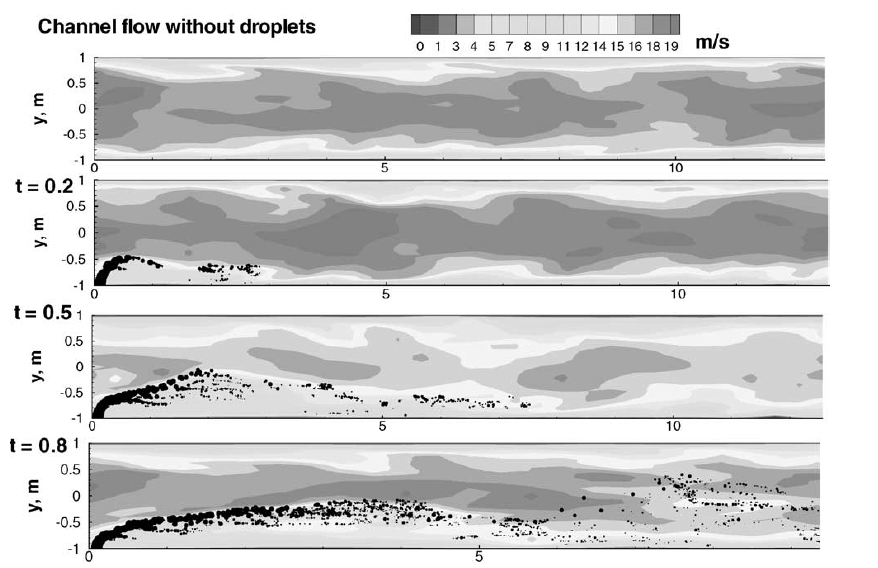
\includegraphics[width=0.75\textwidth]{./part1_numerical_approaches/figures_ch3/apte_2003_jicf}
       \centering
    \caption{Contours of instantenous axial velocity and liquid JICF evolution simulated by \citeColor[apte_les_2003].}
    \label{fig:apte_2003_jicf}
\end{figure}

\subsubsection*{Modeling the liquid-gas interaction with resolved dense core \citepBlackColor[arienti_aerodynamic_2006]}

\citeColor[arienti_aerodynamic_2006] focused their work on capturing the liquid-gas interaction between the liquid column and the gaseous crossflow. For this purpose, they combined a VOF method (see $\S$\ref{subsec:ch2_VOF}) to solve for the dense core with a lagrangian approach to inject and transport droplets. By properly solving for the continuous liquid phase, the blockage effect is directly taken into account without the need of any extra models. Figure \ref{fig:arienti_2006_jicf} left shows front and side views (top and bottom, respectively) of the the dense core resolved by VOF (snapshot a) and of the mean gaseous vector fields at the same planes (snapshot b). Vortices created by the presence of the dense core are captured in both planes with this strategy, hence demonstrating its applicability to model the liquid-gas interaction.

Injection of lagrangian particles is performed at several locations alongside the liquid column, equally space between the nozzle exit and the column breakup point. Droplets sizes are obtained from experimental correlations, while the initial velocity is the continuous phase velocity (i.e. from the liquid column) at the same location plus a fluctuating component obtained as the product between a gaussian PDF and the local turbulent velocity from VOF. Figure \ref{fig:arienti_2006_jicf} right shows a instantaneous snapshot of the spray, showing the dense core and the injected droplets colored by their diameter. Additional submodels considered in the computation include dispersion models to account for turbulent fluctuations during droplets transport \citepColor[gosman_aspects_1983] and the wave secondary atomization model developed by \citeColor[reitz_modeling_1987].


\begin{figure}[ht]
    \centering
    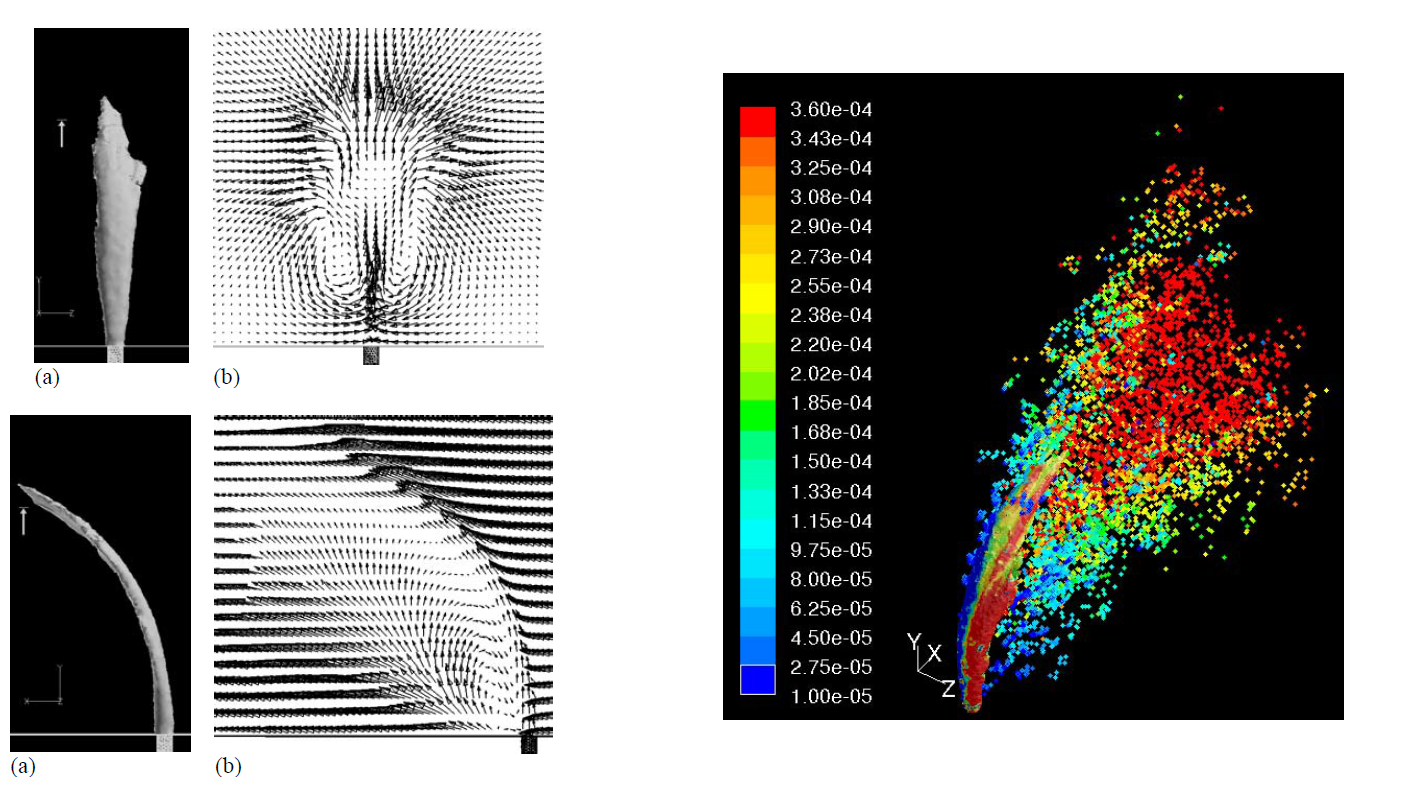
\includegraphics[width=0.7\textwidth]{./part1_numerical_approaches/figures_ch3/arienti_2006_jicf}
       \centering
    \caption[Jet in crossflow simulated with VOF plus lagrangian approach.]{Jet in crossflow simulated with VOF plus lagrangian approach. \textsl{Left}: dense core view and vector lines showing vortical structures. \textsl{Right}: instantaneous snapshot of droplets injected along the dense core. Source: \citeColor[arienti_aerodynamic_2006].}
    \label{fig:arienti_2006_jicf}
\end{figure}


\subsubsection*{Modeling column and shear breakup with empirical laws \citepBlackColor[jaegle_large_2009]}

At operating conditions corresponding to surface breakup (Figure \ref{fig:jicf_breakup_regime_wu}), there are small droplets being torn apart from the liquid column due to the high aerodynamic shear. The quantity of liquid removed by this mechanism is more notorious as $q$ and $We$ are larger. At the same time, there is also the liquid column which undergoes instabilities and breaks first into ligaments (primary atomization) and then into smaller droplets (secondary atomization). Figure \ref{fig:jaegle_senoner_modeling_strategies} left shows both mechanisms of droplet generation.

Some numerical methodologies try to predict the size and flow rate of droplets generated by surface breakup, while simultaneously taking into consideration the liquid column. \citeColor[jaegle_large_2009] has used this strategy by using empirical laws to predict the liquid column, the size of the injected particles and the flow rate of droplets generated by surface breakup. His approach is illustrated in Figure \ref{fig:jaegle_senoner_modeling_strategies} center. Droplets are injected at the injection patch, which corresponds to the liquid nozzle exit. The liquid column is not resolved, but its region of influence is estimated in order to impose a modified drag law to the droplets that are convected within it. Once these droplets abandon the column region, the drag law is changed to the usual one. At the same time, there are droplets being injected along the liquid column region in the axial direction to model the surface breakup mechanism.

The first step in this model is to estimate the region to modify the drag law. For it, the liquid column is assumed to be cylindrical and to expand from the injection location $\left( x_\mathrm{inj}, y_\mathrm{inj}, z_\mathrm{inj} \right)$ until the breakup point $\left( x_\mathrm{b}, y_\mathrm{b}, z_\mathrm{b} \right)$. Its location is estimated from the following experimental expressions by \citeColor[fuller_effects_2000]:

\begin{subequations}
\label{eq:jaegle_breakup_point}
\begin{align}
\frac{x_b - x_\mathrm{inj}}{d_\mathrm{inj}} &= \frac{C_D C_{ab}^2}{\pi} \\
\frac{y_b - y_\mathrm{inj}}{d_\mathrm{inj}} &= 0 \\
\frac{z_b - z_\mathrm{inj}}{d_\mathrm{inj}} &= C_{ab} \frac{u_l}{u_\infty} \sqrt{\frac{\rho_l}{\rho_\infty}}
\end{align}
\end{subequations}

where $C_D = 4.39$ is a constant drag coefficient, $C_{ab} = 2.58$ is a breakup coefficient, $u_l$ is the liquid velocity at injection and $u_\infty$ is the gas freestream velocity. The particles travelling in the liquid column region will follow the following modified transport law \citepColor[fuller_effects_2000]:

\begin{subequations}
\label{eq:momentum_jaegle_model}
\begin{align}
\frac{d u_l}{d t} &= \frac{2 C_D}{d_\mathrm{inj} \pi} \frac{\rho_l}{\rho_\infty} \left( u_\infty - u_l \right)^2  \\
\frac{d v_l}{d t} &= 0 \\
\frac{d w_l}{d t} &= 0 
\end{align}
\end{subequations}

Particles are injected at the $\left( x_\mathrm{inj}, y_\mathrm{inj}, z_\mathrm{inj} \right)$ with  velocity $u_l$ and a size sampled from a distribution obtained experimentally by \citeColor[becker_breakup_2002]. Simultaneously, stripped-off droplets are injected at random locations along the liquid column to account for surface breakup. The mass flow rate $\dot{m}_{l,SB}$ and constant size $SMD_{SB}$ of these droplets are given by the experimental expressions of \citeColor[ranger_aerodynamics_1968] and \citeColor[chou_temporal_1997], respectively:

\begin{subequations}
\label{eq:surface_breakup_jaegle_model}
\begin{align}
\dot{m}_{l,SB} &= \frac{3}{2} l_\mathrm{col} \rho_l \sqrt{\pi d_\mathrm{inj}} A a_l u_\infty \\
SMD_{SB} &= 0.09 d_\mathrm{inj} \\
u_{l,SB} &= u_c + 0.37 \left( u_\infty - u_c \right)
\end{align}
\end{subequations}

where $l_\mathrm{col}$ is the length of the liquid column, $u_c$ is the streamwise velocity of liquid column at the location of surface breakup, and $A$ and $a_l$ are constants obtained from the fluid properties and operating conditions \citepColor[ranger_aerodynamics_1968]. An example of the simulated lagrangian JICF obtained by \citeColor[jaegle_large_2009] is shown in the top of Figure \ref{fig:jaegle_senoner_lagrangian_fields}.

\begin{figure}[ht]
    \centering
    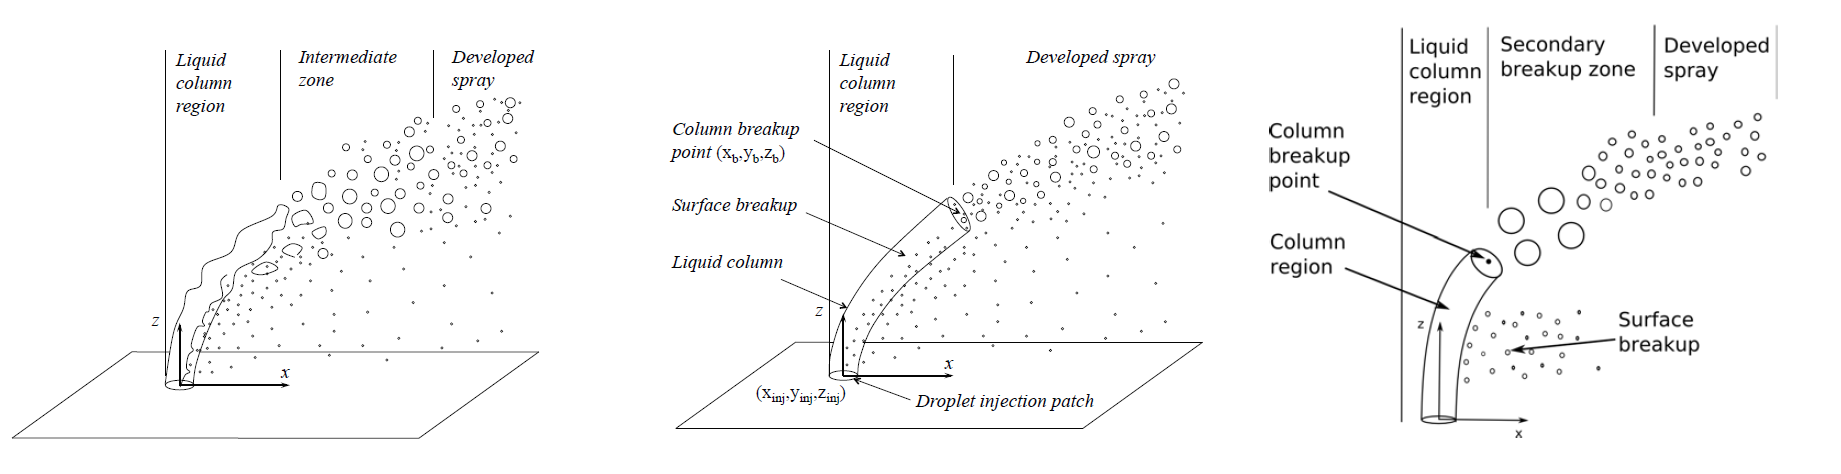
\includegraphics[width=1.0\textwidth]{./part1_numerical_approaches/figures_ch3/jaegle_senoner_modeling_strategies}
       \centering
    \caption[Schemes showing numerical models for liquid jets in crossflow]{Schemes showing numerical models for liquid jets in crossflow. \textsl{Left}: classification of different regions of the liquid jet atomization. \textsl{Center}:  column model considered by \citeColor[jaegle_large_2009], neglecting the intermediate zone and secondary breakup. \textsl{Right}: column model considered by  \citeColor[senoner_simulation_2010].}
    \label{fig:jaegle_senoner_modeling_strategies}
\end{figure}

\subsubsection*{Combining shear breakup with blob method and secondary atomization \citepBlackColor[senoner_simulation_2010]}

A similar approach to the previous one has been explored by \citeColor[senoner_simulation_2010]. In the same way as \citeColor[jaegle_large_2009] (and in the same experimental configuration), the breakup point is calculated from Eqs. (\ref{eq:jaegle_breakup_point}). This location defines then the column region where the modified law of Eqs. (\ref{eq:momentum_jaegle_model}) is applied. Regarding surface breakup, the same methodology used by the previous model is used, where droplets are injected with the properties given in Eqs. (\ref{eq:surface_breakup_jaegle_model}).

The main difference of the approach by \citeColor[senoner_simulation_2010] lies on the size of particles size at injection. While the previous model injects a developed spray, the current one injects big droplets as in the blob method by \citeColor[reitz_modeling_1987], similarly as applied to a JICF case by \citeColor[apte_les_2003] explain previously in this section. In this case, droplets injected at $\left( x_\mathrm{inj}, y_\mathrm{inj}, z_\mathrm{inj} \right)$ have a constant size given by the following expression:

\begin{equation}
d_\mathrm{blob} = \sqrt[3]{\frac{3}{2} d_\mathrm{inj} \lambda_s}
\end{equation}

where $\lambda_s \approx 0.15 d_\mathrm{inj}$ is the wavelength of the column surface instabilities \citepColor[sallam_breakup_2004]. These droplets will then break into smaller sizes by adding a secondary atomization model \citepColor[apte_les_2003]. The present model can then be illustrated as in Figure \ref{fig:jaegle_senoner_modeling_strategies} right. A snapshot of the lagrangian jet obtained by this methodology is shown in Figure \ref{fig:jaegle_senoner_lagrangian_fields} bottom.


\begin{figure}[ht]
    \centering
    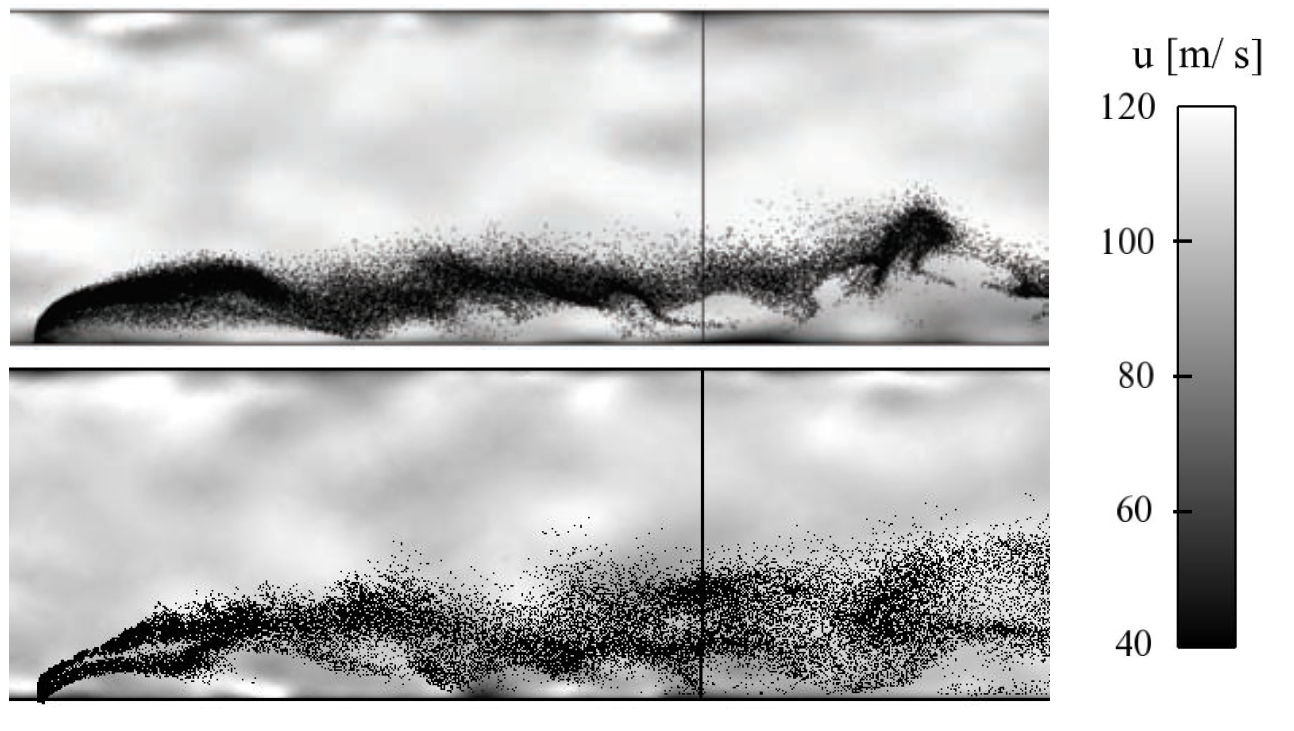
\includegraphics[width=0.6\textwidth]{./part1_numerical_approaches/figures_ch3/jaegle_senoner_lagrangian_fields}
       \centering
    \caption[Instantaneous axial gaseous velocity field on the plane y = 0 mm together with the lagrangian
droplets.]{Instantaneous axial gaseous velocity field on the plane y = 0 mm together with the lagrangian
droplets. q = 6. \textsl{Top}: numerical results by \citeColor[jaegle_large_2009]. \textsl{Bottom}: numerical results by \citeColor[senoner_simulation_2010].}
    \label{fig:jaegle_senoner_lagrangian_fields}
\end{figure}

\subsubsection*{Semi-empirical model for shear breakup regime \citepBlackColor[eckel_semi-empirical_2016]}

Following the line of modeling shear breakup, \citeColor[eckel_semi-empirical_2016] developed a semi-empirical model for this regime. The numerical strategy is depicted in Figure \ref{fig:eckel_2016_modeling_strategy}. This approach injects cylindrical parcels (a,b) mimicking the dense structures of the liquid column which are tracked with a lagrangian formalism and transported with a modified drag law (c). These cylinders have the same diameter as the injection orifice.  As the parcels move, droplets modeling shear breakup are stripped-off the column (d) with properties (mass flow rate, sizes, velocities) given by experimental laws (e). The parcels will then lose mass until they reach a residence time corresponding to the breakup of the liquid column (f), when they are broken into smaller, spherical droplets representing column breakup (g). This approach is continuously performed to model the jet behaviour (h). Dispersion models are used for enhancing the droplet transport \citepColor[gosman_aspects_1983]. Models to account for secondary breakup are not needed, as the employed approach generates a developed spray. A snapshot of the resulting jet is shown in Figure \ref{fig:eckel_2016_jet}, where the difference between the liquid column made of cylindrical parcels and the developed spray zone composed by spherical droplets is clearly visible. 

\begin{figure}[ht]
    \centering
    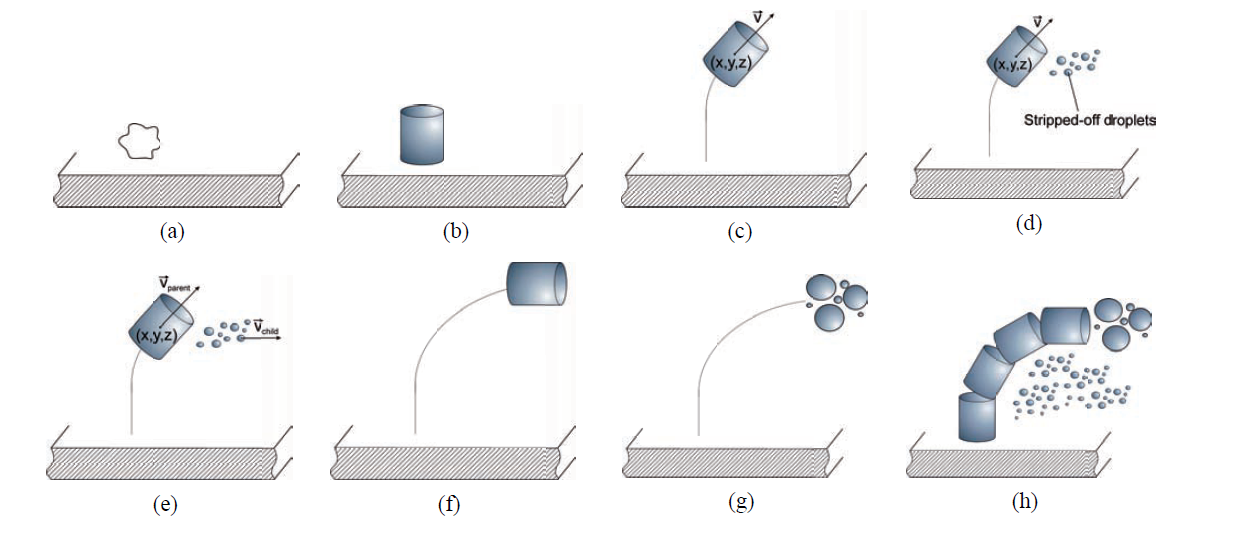
\includegraphics[width=1.0\textwidth]{./part1_numerical_approaches/figures_ch3/eckel_2016_modeling_strategy}
       \centering
    \caption{Jet in crossflow modeling strategy followed by \citeColor[eckel_semi-empirical_2016].}
    \label{fig:eckel_2016_modeling_strategy}
\end{figure}



\clearpage

\begin{figure}[ht]
    \centering
    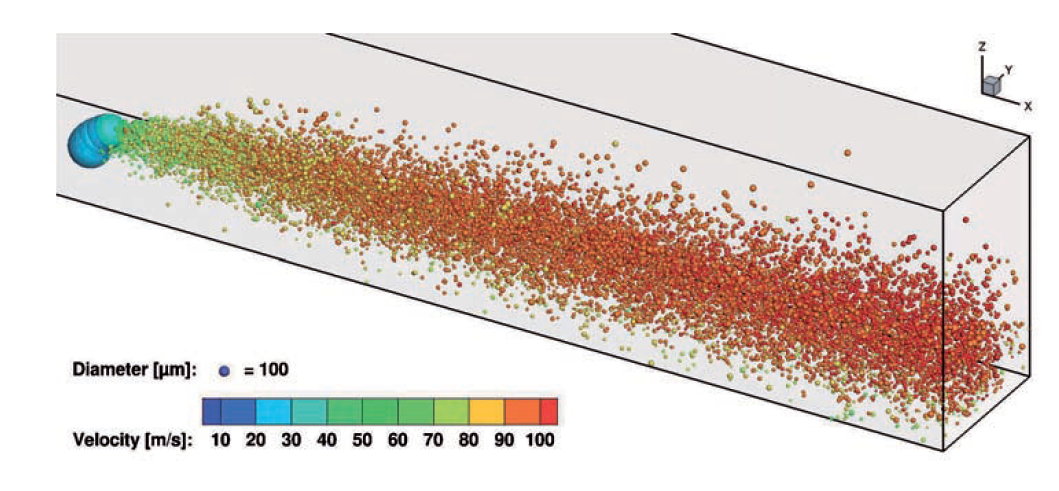
\includegraphics[width=0.6\textwidth]{./part1_numerical_approaches/figures_ch3/eckel_2016_jet}
       \centering
    \caption{Simulation of jet in crossflow by \citeColor[eckel_semi-empirical_2016].}
    \label{fig:eckel_2016_jet}
\end{figure}



\subsubsection*{Statistical method for injection of a fully developed spray \citepBlackColor[fan_eulerianlagrangian_2018]}

From the methodologies discussed previously, all of them except for \citeColor[arienti_aerodynamic_2006] performed injection of droplets at the nozzle orifice center with the liquid injection velocity. Furthermore, large droplets of the order of the nozzle diameter were injected in all cases except in the model of \citeColor[jaegle_large_2009], who introduced a developed spray. In this line, the work of \citeColor[fan_eulerianlagrangian_2018] explored an approach to inject a developed spray at the nozzle orifice following a statistical method. Each particle was injected with attributes chosen as follows:

\begin{itemize}
	
	\item Diameter: sampled from a Probability Density Function (PDF) $f \left(  D \right)$. Four PDFs for droplet sizes were studied: uniform, $\upchi^2$, Nukiyama-Tanasawa and Rosin-Rammler.

	\item Velocity: randomly chosen from a Gaussian distribution with standard deviation equal to the liquid injection velocity.
	
	\item Injection location: at a point randomly located in a circular patch located at the nozzle orifice.

\end{itemize}

Figure \ref{fig:fan_2018_jets_penetration} shows a lateral view of the sprays and the penetration for four cases, each one injecting a different PDF for the droplet diameter. Each PDF gives a different range of droplet diameters and a different spray penetration, showing the importance of chosen accurately the initial boundary conditions for reproducing sprays with lagrangian formalism.

\begin{figure}[ht]
    \centering
    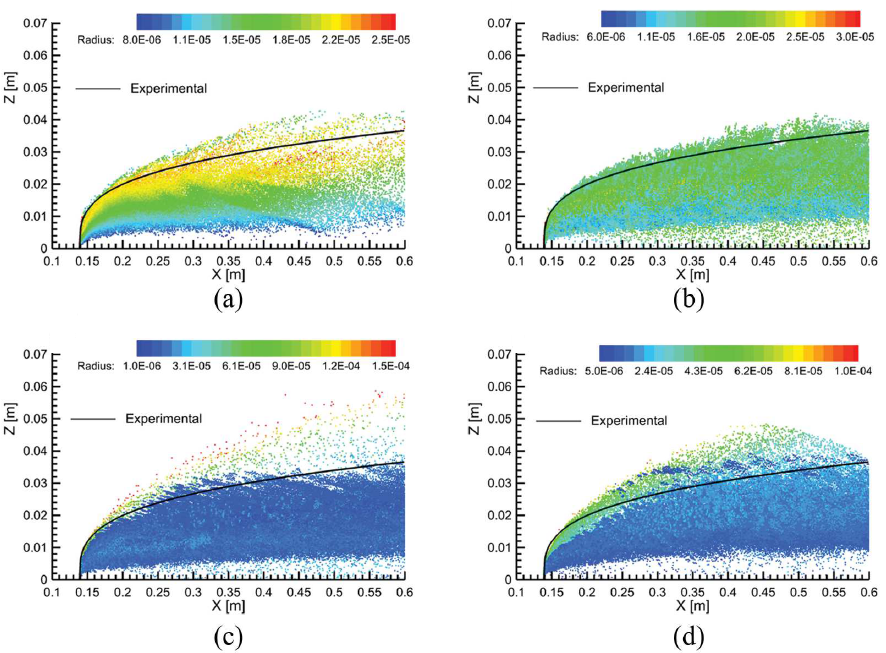
\includegraphics[width=0.7\textwidth]{./part1_numerical_approaches/figures_ch3/fan_2018_jets_penetration}
       \centering
    \caption{JICF sprays and penetrations obtained by \citeColor[fan_eulerianlagrangian_2018] with different injected PDFs for the droplets sizes. (a) Uniform distribution (b) $\upchi^2$ distribution (c) Nukiyama-Tanasawa distribution (d) Rosin-Rammler distribution.}
    \label{fig:fan_2018_jets_penetration}
\end{figure}



\subsubsection*{Hybrid model for jet in crossflow injection \citepBlackColor[fontes_improved_2019]}

One of the most recent works (up to date) focused on JICF modeling has been performed by \citeColor[fontes_improved_2019]. As in the study by \citeColor[arienti_aerodynamic_2006], this approach combines a direct resolution method (VOF) for solving the liquid column with an injection procedure for lagrangian droplets. Experimental correlations are used to obtain column breakup location. The liquid-gas interaction due to the dense core presence is therefore taken into account (Figure \ref{fig:fontes_2019_lagrangian_fields} left). Injection of lagrangian droplets is performed at the column breakup location (Figure \ref{fig:fontes_2019_lagrangian_fields} right): their velocity is equal to the liquid eulerian velocity at this point and their size is obtained from experimental correlations. Two operating points at low $We$ were simulated with this methodology, surface breakup was not modeled since it was not present at these conditions. 

\begin{figure}[ht]
    \centering
    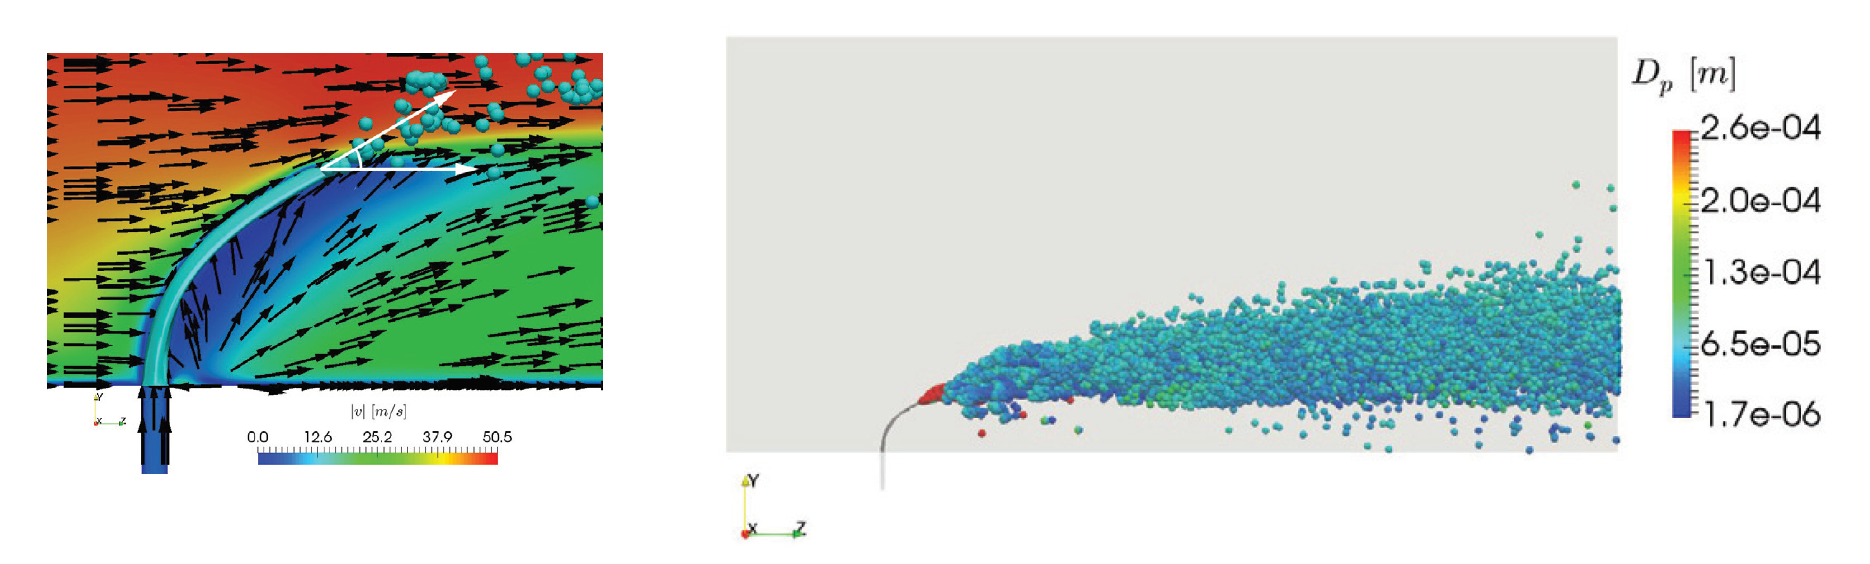
\includegraphics[width=0.9\textwidth]{./part1_numerical_approaches/figures_ch3/fontes_2019_lagrangian_fields}
       \centering
    \caption{Simulated jet in crossflow by \citeColor[fontes_improved_2019]. \textsl{Left}: close view of the near-jet, showing the resolved dense core with VOF and the perturbation effect on the gaseous field. \textsl{Right}: Farfield view of the jet, showing injection point of lagrangian droplets. Droplets are colores by their diameter. }
    \label{fig:fontes_2019_lagrangian_fields}
\end{figure}

 
\newpage





%%----------- Part II: Building SLI  --------------
\part{Building lagrangian injectors from resolved atomization simulations}
%%\include{part2_developments/chapter_JICF}
\chapter{Models for lagrangian injection}
	\label{ch4:sli_development}

\section{Introduction}

Chapter \ref{ch3:disperse_phase_methods} introduced numerical formalisms to represent dispersed two-phase flows. Special emphasis was given to the lagrangian representation of the fluid phase, as it is a widely employed approach in aerospace applications due to its low computational cost with respect to other formalisms and its ability to account for extra physics such as collisions, evaporation and combustion. The chapter culminated with the presentation of lagrangian models to model fuel injection in MSFI systems, giving extra attention to the state of the art in methodologies for simulating JICF. 

In this work, a novel numerical methodology to build numerical injectors for performing dispersed phase simulations in MSFI systems has been developed. The injectors built with this methodology have been baptised as Smart Lagrangian Injectors (SLI). Figure \ref{fig:state_art_injection} shows the location of the new method into the proposed classification of existing numerical models for lagrangian injection: SLI are built by learning a reference spray, which can be obtained either experimentally or numerically. In this thesis, the reference spray is obtained through resolved simulations of the atomization process. Computations performed with SLI will also account for the interaction of the dense liquid phase with the surrounding gas (blockage effect in liquid JICF) and secondary atomization models for further breakup of lagrangian particles.

This chapter details the underlying theory of SLI, showing all the key modeling ingredients. Section \ref{sec:ch4_spray_description} introduces mathematical foundations representing the spray which are used by describing the models in Section \ref{sec:ch4_models_flowchart}. The learning methodology to build injectors from a reference spray is defined in Section \ref{sec:ch4_SLI_learning}. Finally, the theory of the models blocks accounting for the blockage effect and secondary atomization models are discussed respectively in Sections \ref{sec:ch4_dense_core_modelling} and \ref{sec:ch4_secondary_atomization_modeling}.
 

%In this work, this new methodology has been applied to model liquid JICF injection, whose reference spray for the learning process has been obtained by performing resolved simulations of atomization with an academic test case. The results of these simulations are shown in Chapter \ref{ch5:jicf_resolved_simulations}. In a latter step, the SLI built from these simulations are applied to initialise dispersed phase computations for the same configuration in Chapter \ref{ch6:jicf_lgs_simulations}. Finally, all the methodology is applied in Part \ref{part3:BIMER} to a multipoint burner.



\section{Mathematical description of sprays}
	\label{sec:ch4_spray_description}

In $\S$\ref{subsec:ch3_statistical_methods}, dispersed sprays resulting from atomization were described by a function $f$ which represented the number density function of droplets. Then, all spray characteristics can be obtained by a proper definition and integration of $f$. Several methods targeting the determination of $f$ were discussed in Chapter \ref{ch3:disperse_phase_methods}, from statistical approaches to the LPP representation. Even if only statistical approaches make use of the WBE formulation, LPP can be considered as an approximation to the $f$ function by considering the point particle approximation. Consequently, since in this work the LPP representation is chosen to represent dispersed phase flows, a mathematical representation of dispersed sprays based on the function $f$ as given by Eq. (\ref{eq:f_spray_description_subramanian}) is used. This section intends to provide some theoretical foundations for the developed models from a generic, mathematical perspective. The rest of the chapter will be dedicated to explain how this formulation is applied in the current work. \\

\clearpage

\subsection{General formulation}

The spray produced by atomization can be described by a continuous function $F$:

\begin{equation}
F \left( t, \textbf{x}, \textbf{u}, D \right) 
\end{equation}

which is defined in the whole spatial domain $\Omega \left( \boldsymbol{x} \right)$, $\forall \boldsymbol{x} = \left\lbrace x, y, z \right\rbrace^T \in {R}^3$. In this first version of SLI, the spray will be characterized in plane surfaces. Therefore, it is of interest to sample the spray crossing a surface $\mathcal{S}$ belonging to the whole spatial domain: $\mathcal{S} \subset \Omega $. The spray sampled in this surface is described by a continuous function $f$:

\begin{equation}
\label{eq:f_general}
 f \left( t, \textbf{x}, \textbf{u}, D \right) = F \left( t, \textbf{x}, \textbf{u}, D \right) ~ \forall ~ \textbf{x} \in \mathcal{S}
\end{equation}

As $f$ is defined in a surface, it can be spatially represented by only two coordinates. These surface coordinates can be expressed as a vector $\boldsymbol{s} = \left\lbrace \xi, \eta \right\rbrace$. They can represent any type of surface, from cartesian to curvilinear. Therefore, the function $f$ can be expressed in terms of $\boldsymbol{s}$ as:

\begin{equation}
\label{eq:f_surface_coordinates}
f \left( t, \boldsymbol{s}, \textbf{u}, D \right)  
\end{equation}

Since both Eqs. (\ref{eq:f_general}) and (\ref{eq:f_surface_coordinates}) are identical, there is an equivalence between $\boldsymbol{x} = \left\lbrace x, y, z \right\rbrace$ and $\boldsymbol{s} = \left\lbrace \xi, \eta \right\rbrace$. This relation can be expressed mathematically as:

\begin{equation}
\label{eq:morphism_general_definition}
h : \boldsymbol{x} \rightarrow \boldsymbol{s}
\end{equation}

% Cool about morphisms: https://www.euclideanspace.com/maths/discrete/structure/map/morphism/index.htm

where $h$ is a mapping function, or morphism, that will transform from cartesian coordinates $\boldsymbol{x}$ to surface coordinates $\boldsymbol{s}$. \\


In this work, the variation of the spray characteristics with time will not be considered. Instead, the obtention and study of a stationary, mean spray will be the main objective of SLI. For such purpose, the spray will be sampled in time for a period $T$ which should be large enough in order to obtain a converged spray (see $\S$\ref{subsec:SLI_spray_convergence}), hence eliminating the dependence with time. Mathematically speaking, this can be represented through integration:

\begin{equation}
\label{eq:f_general_time_integrated}
f \left( \boldsymbol{s}, \boldsymbol{u}, D \right) = \frac{1}{T} \int_0^T f \left( t, \boldsymbol{s}, \boldsymbol{u}, \right) dt
\end{equation}

Eventually, for a better characterization of the spray, the sampling surface $\mathcal{S}$ will be spatially discretized into several elements, or probes, of size $\Delta S$. In this way, the spray within each probe can be independently study to provide \textbf{spatially refined statistics}. The representation of spatially refined statistics can be obtained from $f$ by integrating spatially this function within each probe with center $\left( \xi_\mathrm{j}, \eta_\mathrm{k} \right)$:

\begin{equation}
\label{eg:f_discrete}
f_\mathrm{j,k} \left( \boldsymbol{s}_\mathrm{j,k}, \boldsymbol{u}, D \right) = \frac{1}{\Delta \xi \Delta \eta} \int_{\xi_\mathrm{j-1/2}}^{\xi_\mathrm{j+1/2}} \int_{\eta_\mathrm{k-1/2}}^{\eta_\mathrm{k+1/2}}  f \left( \boldsymbol{s}, D \right) d\xi d\eta
\end{equation}

\subsection{Spray formulation in jet in crossflow}

A more precise, less abstract interpretation for the SLI spray formulation can be obtained by applying the general formulation to a liquid JICF problem, atomication case introduced in $\S$\ref{sec:ch1_fuel_injection_technology}. Figure \ref{fig:JICF_spray_formulation} shows a liquid JICF from a resolved atomization simulation. As observed, the liquid leaves the injection nozzle as a coherent jet moving along the $z$ direction and then starts bending towards the $x$ direction. Atomization starts taking place and breaks the jet into firstly ligaments and, subsequently, droplets. The resulting droplets from the atomization process conform a spray that can be analyzed by the SLI strategy. Therefore, to study this spray, first droplets need to be sampled in sampling surfaces. In a geometrically simple JICF problem as the one from Figure \ref{fig:JICF_spray_formulation}, the sampling surfaces are planes perpendicular to the crossflow direction $x$ denoted in the figure by $S$. The surface coordinates $\boldsymbol{s}$ aforementioned correspond therefore to the in-plane coordinates in the sampling surface, which in the system of reference depicted in Figure \ref{fig:JICF_spray_formulation} yield $\boldsymbol{s} = \left\lbrace y, z \right\rbrace$. Therefore the discrete, spatially refined statistics are obtained in probes centered at $\left( y_\mathrm{j}, z_\mathrm{k} \right)$, and the function $f_\mathrm{j,k}$ given generally by Eq. (\ref{eg:f_discrete}) can be applied to the proposed JICF formulation as:

\begin{equation}
\label{eg:f_discrete_jicf}
f_\mathrm{j,k} \left( \boldsymbol{s}_\mathrm{j,k}, \boldsymbol{u}, D \right) = \frac{1}{\Delta y \Delta z} \int_{y_\mathrm{j-1/2}}^{y_\mathrm{j+1/2}} \int_{z_\mathrm{k-1/2}}^{z_\mathrm{k+1/2}}  f \left( \boldsymbol{s}, \boldsymbol{u}, D \right) dy dz
\end{equation}

\begin{figure}[h!]	
	\centering
	\includeinkscape[inkscapelatex=false,scale=0.6]{./part2_developments/figures_ch4_SLI/JICF_spray_formulation}
	\caption{Illustration of SLI spray formulation in a liquid JICF.}
	\label{fig:JICF_spray_formulation}
\end{figure}


\section{Models for lagrangian injection}
	\label{sec:ch4_models_flowchart}
	
The objective of the models 	for performing lagrangian injection is to provide the necessary input parameters to initialize disperse-phase simulations. These input parameters are intended to represent a realistic spray resulting from primary atomization. Most existing models perform lagrangian injection by neglecting the atomization process due to its complexity, while other rely on experimental data or correlations which are valid for a limiting range of operating conditions (see $\S$\ref{sec:ch3_state_art_lagrangian_injection} for a discussion on the state of the art in dispersed-phase simulations of MSFI systems). 

With this objective in mind and knowing the limitations of the existing approaches, the intention of this work is to develop models that can be fed from primary atomization data to: 1) inject a proper dispersed-phase and 2) model as accurately as possible the momentum exchange due to the liquid-gas interaction in the primary atomization region. The second point has often been neglected in many dispersed phase simulations, and has been the object of multiple studies dealing with primary atomization. To address both points, this thesis relies firstly on \textbf{numerical simulations of the resolved atomization process} using an ACLS/AMR approach ($\S$\ref{subsec:ch2_ACLS}). These simulations are used to construct a spray database by sampling the droplets passing through planes perpendicular to the crossflow direction and then applying the spray formulation previously presented. The functions $f \left( \boldsymbol{s}, \boldsymbol{u}, D \right) $ of the spray formulation represent therefore the statistical distributions of the spray's size, velocity and fluxes that are processed in a \textbf{lagrangian injectors learning process} to eventually yield the discretized spray $f_\mathrm{j,k} \left( \boldsymbol{s}_\mathrm{j,k}, \boldsymbol{u}, D \right)$ that is used as lagrangian injector to initialize \textbf{dispersed-phase simulations}. At the same time, the liquid-gas interaction between the jet dense core and the crossflow is also analyzed and learnt to provide a model that contributes to the liquid-gas \textbf{momentum exchange} in the disperse-phase simulations, which a priori is neglected (and which many models do not take into account or circumvent by introducing experimental correlations). In this way, the full methodology currently relies only on the data from the resolved atomization simulations in order to fully initialize dispersed-phase computations. Therefore, any operating point could be simulated through resolved simulations and learnt with the proposed methodology without the need of relying on experimental data or semi-empirical correlations. The proposed approach will be called hereafter as Smart Lagrangian Injectors (SLI).

The full approach of SLI is detailed schematically in the flowchart of Figure \ref{fig:SLI_graphic_description}. The process is summarized in the following lines:


\begin{enumerate}

	\item \textbf{Resolved atomization simulations} are performed to build a spray (statistical spray distributions) and liquid-gas interaction (momentum exchange) database (Chapter \ref{ch5:jicf_resolved_simulations}).
	
	\item This database is used and processed by the models to \textbf{learn the spray state} and build lagrangian injectors (Chapter \ref{ch4:sli_development}). The learning part consists of the following parts: \textbf{spray sampling} ($\S$\ref{subsec:SLI_spray_sampling}), \textbf{spatial discretization} ($\S$\ref{subsec:SLI_spatial_discretization}) and \textbf{spray convergence} ($\S$\ref{subsec:SLI_spray_convergence}) of the injectors. The convergence can be checked either globally in the sampling plane, or locally by dealing with the sprays contained in each discrete, individual probe in order to perform a \textbf{converge-driven classification} ($\S$\ref{subsec:SLI_quadtrees_discretization}).
	
	\item \textbf{Dispersed-phase simulations} are initialized with the injectors developed with this methodology (Chapter \ref{ch6:jicf_lgs_simulations}). Apart from the lagrangian injectors that inject the liquid phase, the two following submodels are also contained in these simulations: 
	
		\begin{itemize}
	
		\item \textbf{Dense core learning} with the \textbf{actuator line model} in order to take into account the perturbation effect of the liquid dense structures (i.e. the liquid dense core in the JICF) in the gaseous phase during lagrangian simulations ($\S$\ref{sec:ch4_dense_core_modelling}). The information to characterize the dense core is taken from the resolved simulations and later imposed into lagrangian ones.
		
		\item \textbf{Secondary atomization models} to consider further possible breakup of spherical droplets during lagrangian simulations ($\S$\ref{subsec:SLI_spatial_discretization}).
		
		\end{itemize}


\end{enumerate}


\begin{figure}[h!]	
	\centering
	\includeinkscape[inkscapelatex=false,scale=0.3]{./part2_developments/figures_ch4_SLI/SLI_graphic_description_with_learning_boxes}
	\caption{Flowchart of the SLI formulation applied to liquid JICF.}
	\label{fig:SLI_graphic_description}
\end{figure}


%
%\section{Models for lagrangian injection (OLD)}
%	\label{sec:ch4_models_flowchart}


%\begin{figure}[h!]	
%	\centering
%	\includeinkscape[inkscapelatex=false,scale=0.3]{./part2_developments/figures_ch4_SLI/SLI_graphic_description}
%	\caption{Illustration of SLI working principle \textbf{CHANGE FIGURE TO NEW CONFIG WITHOUT SIDE WALLS}.}
%	\label{fig:SLI_graphic_description}
%\end{figure}




%\begin{figure}[h!]	
%	\centering
%	\includeinkscape[inkscapelatex=false,width=17cm]{./part2_developments/figures_ch4_SLI/SLI_flowchart_with_pictures}
%	\caption{Flowchart for proposed models of lagrangian injection.}
%	\label{fig:SLI_flowchart}
%\end{figure}




\section{Lagrangian injectors learning}
	\label{sec:ch4_SLI_learning}


\subsection{Spray sampling}
\label{subsec:SLI_spray_sampling}

\subsubsection*{Identification of liquid structures in resolved simulations}

The first step in the learning process is to obtain the spray from resolved atomization simulations. For this purpose, droplets must be identified in space. According to the ACLS methodology ($\S$\ref{subsec:ch2_ACLS}), liquid regions are identified by level set values $\psi > 0.5$, and the interface $\Gamma$ is located at $\psi = 0.5$. It is possible then to identify and tag individual liquid structures as independent closed regions of $\Gamma$, whose domain is denoted as $\Omega_l$. Each structure can then be characterized by its volume $V_\mathrm{dr}$, its center of mass location $\textbf{x}_\mathrm{dr}$ and velocity $\textbf{u}_\mathrm{dr}$, and maximum and minimum distances from the interface to the center of mass $R_\mathrm{max}$ and $R_\mathrm{min}$, as depicted in Figure \ref{fig:droplet_sampling_parameters}. The formulas used for calculating these parameters are shown in Table \ref{tab:sampling_parameters}. 

\begin{table}[!h]
\centering
\caption{Parameters sampled from resolved atomization simulation}
\begin{tabular}{ccl}
\thickhline
Parameter & Definition & Description \\
\thickhline
$V_\mathrm{dr}$ & $\displaystyle \int_{\Omega_l} d V$ & Volume enclosed by interface  \\
\hline
$\textbf{x}_\mathrm{dr}$ & $\displaystyle \frac{1}{V} \int_{\Omega_l} \boldsymbol{x} d V$ &   Location of center of mass \\
\hline
$\textbf{u}_\mathrm{dr}$ & $\displaystyle \frac{1}{V} \int_{\Omega_l} \textbf{u} \left( \boldsymbol{x} \right) d V$ & Velocity of center of mass  \\
\hline
$r_\mathrm{max}$ & $\displaystyle \max \left( | \textbf{x} - \textbf{x}_\mathrm{dr} | \right) \forall \textbf{x} \in \Omega_l$ & Maximum distance to center of mass \\
\hline
$r_\mathrm{min}$ & $\displaystyle \min \left( | \textbf{x} - \textbf{x}_\mathrm{dr} |  \right) \forall \textbf{x} \in \Omega_l$ & Minimum distance to center of mass \\
\thickhline
\end{tabular}
\label{tab:sampling_parameters}
\end{table}

\begin{figure}[h!]	
	\centering
	\includeinkscape[inkscapelatex=false,scale=0.5]{./part2_developments/figures_ch4_SLI/droplet_sampling_parameters}
	\caption{Parameters characterizing liquid structures sampled in resolved atomization simulations. }
	\label{fig:droplet_sampling_parameters}
\end{figure}

In order to get statistics for spray characterization, it is useful to define a characteristic size of each liquid structure. For this purpose, an equivalent radius $r_\mathrm{dr}$ is calculated from the liquid volume $V_\mathrm{dr}$:

\begin{equation}
\label{eq:ch4_r_equivalent_calculation}
r_\mathrm{dr} = \sqrt[3]{\frac{3 V_\mathrm{dr}}{4 \pi}}
\end{equation}

which is the radius of a sphere containing the same volume as the liquid structure. The equivalent diameter is then $d_\mathrm{dr} = 2 r_\mathrm{dr}$. In cases where sampled structures are spherical droplets, $R_\mathrm{dr}$ is the true radius and, therefore, a representative measure of the droplets' size. On the other hand, if liquid structures are not fully spherical (which is often the case after primary atomization), the equivalent radius does not provide full information on their topology. To determine the deviation of the identified liquid structure from a sphere, the radii $r_\mathrm{max}$ and $r_\mathrm{min}$ can be used to calculate the deformation parameters $\alpha$ and $\beta$ \citepColor[zuzio_improved_2018]:

\begin{equation}
\label{eq:ch4_deformation_parameters_alpha_beta_calculation}
\alpha = \frac{r_\mathrm{max}}{r_\mathrm{dr}} ~~ ; ~~ \beta = \frac{r_\mathrm{min}}{r_\mathrm{dr}}
\end{equation}	

By definition, $\alpha \geq 1$ and $\beta \leq 1$. A perfect sphere would present $\alpha = \beta = 1$.

In this work, no distinction between droplets and ligaments has been done to construct the injectors after the learning procedure. Hence, hereafter all liquid structures will be referred as droplets, and the term droplet sampling will be used. Inclusion of distinction between ligaments and droplets (i.e. between non-spherical and spherical structures) could be further taken into account with parameters $\alpha$ and $\beta$ to, for example, modify drag coefficients in lagrangian simulations at the first steps after injection \citepColor[bagheri_drag_2016]. 


\subsubsection*{Sampling procedure}

Droplets are sampled according to their center of mass (CM) location. Note that, despite the ACLS methodology being eulerian, liquid structures produced by resolved simulations are being tracked as lagrangian particles (lagrangian tracking). Two sampling methods based on experimental techniques can be used \citepColor[tropea_optical_2011], their main difference being the topology of the sampling regions (see Figure \ref{fig:tropea_droplet_sampling}):

\begin{itemize}

	\item A control volume (unit volume in Figure \ref{fig:tropea_droplet_sampling}) can be defined where particles contained inside are sampled at a particular time instant. This method produces a \textbf{volume distribution}. 
	
	\item A surface area (unit area in Figure \ref{fig:tropea_droplet_sampling}) or plane where droplets crossing it during a given time are sampled. A \textbf{flux density distribution} is obtained in this case.

\end{itemize}


\begin{figure}[h!]
	\centering
	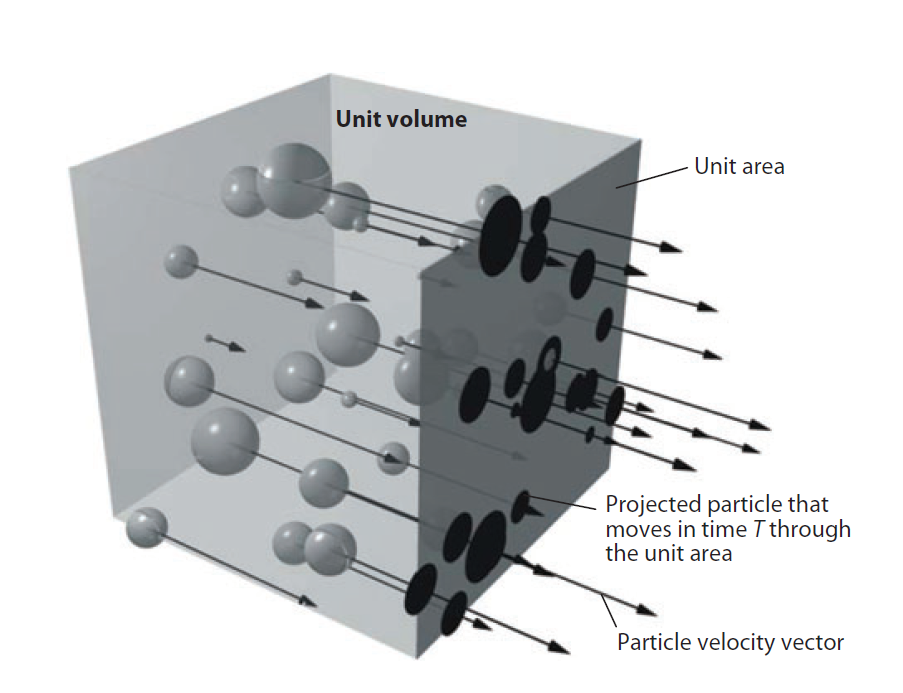
\includegraphics[scale=0.6]{./part2_developments/figures_ch4_SLI/tropea_droplet_sampling}
	\caption{Droplet sampling prodecure. Source: \citeColor[tropea_optical_2011]}
	\label{fig:tropea_droplet_sampling}
\end{figure}

In this work, droplets crossing surface areas are sampled, hence obtaining flux density distributions. This method is chosen to be closer to experimental measurements performed in jet in crossflow configurations \citemColor[wu_spray_1998,becker_breakup_2002]. The defined surface areas employed will be hereafter referred as \textbf{sampling planes}. To determine when a droplet is sampled, a sampling rate $T_\mathrm{sample}$ is specified so that the current location and velocities of droplets CM at time $t$ is checked. Then, the location of each droplet at time $t + T_\mathrm{sample}$ is estimated by projecting the position of the center of mass with the current velocities. Droplets whose current location at $t$ and projected location at $t + T_\mathrm{sample}$ is at different sides of a sampling plane are sampled. This procedure is referred as \textbf{lagrangian projection} of droplets. It is computationally cheap, so can be performed in the resolved and dispersed phase computations without highly increasing the cost of the simulations. On the other hand, it has the main disadvantages that: 1) some actual crossing droplets might not be sampled and 2) contrarily, some droplets might be sampled twice. These downcomes of the methodology could be circumvented by including a tag field in the resolved simulations where droplets are assigned an ID number that does not change with time. However, this is not available yet and is difficult to implement, since the atomization process hinders droplet tagging as liquid structures change constantly during primary and secondary breakup.

The sampling rate is chosen so that that all droplets crossing the plane are collected. Droplets are accumulated with time, and then statistics are calculated. Choosing a right sampling rate ensures that at the end of the accumulation process, the mass flow rate in average is the actual rate passing through the sampling plane in the resolved simulations. If the sampling rate is too low, some droplets might be missed and the flow rate captured will not be the right one (aliasing phenomenon on the spray sampling procedure). Another technique to measure flow rates directly in resolved atomization simulations, called interior boundaries, has been developed in this thesis. This one is later explained in $\S$\ref{subsec:ch5_interior_boundaries} and compared to the rates obtained from the lagrangian tracking procedure in $\S$\ref{subsec:ch5_sli_fluxes_vs_IBs}. \\

\subsubsection*{Defining statistics for sprays}

The resulting accumulated spray is composed of a polydisperse ensemble of droplets, each droplet characterized by parameters from Table \ref{tab:sampling_parameters}. In order to characterize the spray, it is useful to define averaged and Root-Mean Squared (RMS) values for the whole spray from the individual droplets parameters. For an arbitraty magnitude $f$, the arithmetic mean and RMS values would be defined as follows:

\begin{equation}
\label{eq:ch4_f_arbitrary_mean_RMS_definition}
\overline{f} = \frac{1}{N_\mathrm{dr}} \sum_{i=1}^{N_\mathrm{dr}} f_i  ~~~~~~ ; ~~~~~~ f_\mathrm{RMS} = \sqrt{\overline{f^2} - \overline{f}^2}
\end{equation}

%\begin{equation}
%\overline{f} = \frac{1}{T} \sum f_i \Delta t_i ~~~~~~ ; ~~~~~~ f_\mathrm{RMS} = \sqrt{\overline{f^2} - \overline{f}^2}
%\end{equation}

where $N_\mathrm{dr}$ is the number of accumulated droplets. In the case of polydisperse sprays, where there are several liquid structures with different volumes, it is also useful to define volume-weighted averages in order to give more relevance to the properties of larger droplets. For an arbitrary magnitude $f$, the volume-weighted mean and RMS can be defined as:

\begin{equation}
\label{eq:ch4_f_arbitrary_mean_RMS_VW_definition}
\displaystyle \overline{f}_\mathrm{VW} = \frac{1}{\sum_{i=1}^{N_\mathrm{dr}} V_i} \sum_{i=1}^{N_\mathrm{dr}} f_i V_i ~~~~ ; ~~~~ f_\mathrm{RMS,VW} = \sqrt{\displaystyle \overline{f^2 }_\mathrm{VW} - \displaystyle \overline{f }_\mathrm{VW}^2}
\end{equation}

where $V_i$ is the volume of each liquid structure. Related to the injectors the definition of mean and RMS values, either arithmetic or weighted-averaged, will be applied to the velocities in the three directions, $\alpha$ and $\beta$. \\

In two-phase flow problems involving disperse-phase sprays, it is useful to define average diameters of droplets with definitions different than the one given by applying Eq. (\ref{eq:ch4_f_arbitrary_mean_RMS_definition}). since they are better representative of the physical problems involving mass or heat transfer \citepColor[lefebvre_atomization_2017]. For combustion applications, the most used averaged diameter is the Sauter Mean Diameter (SMD):

\begin{equation}
\label{eq:ch4_SMD_definition}
\mathrm{SMD} = \frac{\sum_{i=1}^{N_\mathrm{dr}} d_i^3 }{\sum_{i=1}^{N_\mathrm{dr}} d_i^2}
\end{equation} 

where $d_i$ is the individual diameter of each droplet. The numerator of this expression is proportional to the cube of the diameter, which is equivalent to the droplet volume. The denominator is dependent to its square, which is related to the droplet liquid surface. Therefore, the SMD represents the relation between the liquid volume and surface in a spray. This is specially useful when evaporation is present (i.e. prior to combustion), since evaporation occurs when the specific liquid surface (the surface of liquid in contact with air) is large: that is, when the SMD is small.

Finally, a last useful magnitude that can be defined for a convecting spray is the liquid flow rate, which is a mean quantity by definition. Considering a sampling surface as in Figure \ref{fig:tropea_droplet_sampling}, the mean liquid flow rate passing through it can be obtained as:

\begin{equation}
\label{eq:ch4_Ql_definition}
Q_l = \frac{d V_l}{dt} \approx \frac{\Delta V_l}{\Delta t} = \frac{\sum_{i=1}^{N_\mathrm{dr}} V_i}{t_\mathrm{acc}} 
\end{equation}

where $t_\mathrm{acc}$ is the total accumulation time. $Q_l$ yields an absolute flux that represents the mass flux passing through each sampling plane considered. If the sampling plane is discretized in several probes (see $\S$\ref{subsec:SLI_spatial_discretization}) and the fluxes are determined within them, the addition of all probes' fluxes will yield the absolute flux from the whole sampling plane. In these cases, the fluxes from each probe will depend on the probes surface $S_\mathrm{probe}$: the smaller $S_\mathrm{probe}$, the smaller the absolute flux. Therefore, when dealing with spatially discretized sprays it is useful to express the absolute flux in relation $S_\mathrm{probe}$. This yields a surface-weight flux $q_l$, named also volume flux:

\begin{equation}
\label{eq:ch4_volume_flux_definition}
q_l = \frac{Q_{l,\mathrm{probe}}}{S_\mathrm{probe}}
\end{equation}

The value of $q_l$ converges with the probe size, as opposed to $Q_l$. Effectively, if the size of the probe $\Delta y \times \Delta z$ is reduced, the liquid flux as defined by Eq. (\ref{eq:ch4_Ql_definition}) will also decrease since less droplets might be sampled in a smaller surface. Nevertheless, the volume flux $q_l$ defined by Eq. (\ref{eq:ch4_volume_flux_definition}) will we maintaned because, despite the reduction in $Q_l$, the probe surface is also smaller.

\clearpage

%The in-plane, accumulated spray is discretized with a grid composed of uniform probes with surface $S_\mathrm{probe}$. For each probe, a surface-weight flux can be calculated. Denoted as $q_l$, it can be obtained as:
%
%\begin{equation}
%\label{eq:ch4_Ql_definition}
%q_l = \frac{Q_l}{S_\mathrm{probe}}
%\end{equation}

%The advantage of $q_l$ is that it converges with the probe size, as opposed to $q_l$. Effectively, if the size of the grid $\Delta y$ x $\Delta z$ is reduced, the liquid flux as defined by Eq. (\ref{eq:ch4_Ql_definition}) will also decrease since less droplets might be sampled in a smaller surface. Nevertheless, the volume flux $q_l$ will we maintaned because, despite the reduction in $Q_l$, the probe surface is also smaller.



\subsection{Spray convergence}
\label{subsec:SLI_spray_convergence}

Simulations using the ACLS/AMR methodology resolve atomization and provide deep insight on the driving physical phenomena. Nevertheless, their main limitation is their cost (see $\S$\ref{subsec:ch5_computational_performances}), which increases when more liquid is present in the domain. Consequently, the accumulation time of droplets will be finite and, logically, restricted to the physical time simulated. This can pose a problem for spray characterization, since statistics might not be converged if the number of sampled droplets is not sufficient.

Here, a methodology to evaluate spray convergence is proposed. The objective is to provide a quantitative measure to assess whether enough droplets have been sampled to obtain reliable statistics \citepColor[vie_particle-laden_2016]. If the spray is converged, then it can be spatially discretized to get local statistics that will conform the injectors ($\S$\ref{subsec:SLI_spatial_discretization}). This convergence criterion is also used to propose another discretization strategy in which refinement is performed following a quadtrees structure (convergence-driven discretization, see $\S$\ref{subsec:SLI_quadtrees_discretization}).

At each time step $t_i$ of the accumulation process, the spray will be formed by a number of droplets $N_{\mathrm{dr},i}$. This number will increase as more particles are accumulated with time, since all droplets sampled previously are also accounted for (hence the name accumulation). One can see this methodology as obtaining a \textbf{time-averaged spray}, since dependence with time is neglected. Statistics representing the spray, such as droplet size histograms, can be calculated on the accumulated spray at each time $t_i$. Figure \ref{fig:spray_convergence_description_accumulation_and_MSE_comparison} left shows an illustrated view of the size histogram evolution at several accumulation instants. The histogram indicates thes probability $f \left( d_\mathrm{dr} \right)$ of finding a droplet of size $d_\mathrm{dr}$ within a class $n$: $d_\mathrm{dr} \in \left[ d_{\mathrm{dr},n}-\Delta d_\mathrm{dr}/2, d_{\mathrm{dr},n}+\Delta d_\mathrm{dr}/2 \right]$. Its shape will change with accumulation time until an instant from which it will stay constant if more droplets are sampled. At this point, the spray will be considered to be converged. 

\begin{figure}[ht]
     \centering
     \begin{subfigure}[b]{0.45\textwidth}
         \centering
         \includeinkscape[inkscapelatex=true,scale=0.35]{./part2_developments/figures_ch4_SLI/size_distribution_evolution_with_accumulation}
     \end{subfigure}
     %\hfill
     \begin{subfigure}[b]{0.45\textwidth}
         \centering
          \includeinkscape[inkscapelatex=true,scale=0.45]{./part2_developments/figures_ch4_SLI/size_distribution_histograms_comparison}
     \end{subfigure}
        \caption{\textsl{Left}: Size histogram evolution with accumulation time of droplets. \textsl{Right}: comparison of two droplet size histograms from two consecutive time instants.}
	% See: https://stackoverflow.com/questions/35210337/can-i-plot-several-histograms-in-3d/35225919
        \label{fig:spray_convergence_description_accumulation_and_MSE_comparison}
\end{figure}



The main issue now is to determine quantitatively when the spray is converged. For this purpose, the histograms are compared in pairs at subsequent time instants, $t_i$ and $t_{i-1}$, as shown in Figure \ref{fig:spray_convergence_description_accumulation_and_MSE_comparison} right. The same number and width of droplets classes are used in both histograms. The difference between both histograms is then measured by means of a Mean Squared Error (MSE) function defined as:

\begin{equation}
\label{eq:MSE_definition}
MSE^{t_i} = \frac{1}{N} \sum_{n=1}^N \left( f_n^{t_{i-1}} - f_n^{t_i}  \right)^2
\end{equation}

where $N$ is the total number of classes in the histogram. This criterion is similar to the Cramer-von Mises measure to compare two statistical distributions \citepColor[anderson_distribution_1962]. The MSE can then be calculated at each accumulation time instant and then be normalized by the maximum value obtained, yielding a Normalized Mean Squared Error (NMSE) \citepColor[hanna_flacs_2004]:

\begin{equation}
NMSE^{t_i} = \frac{MSE^{t_i}}{\max_{t_i} \left( MSE \right)}
\end{equation}

The evolution of NMSE can be displayed with time as shown in Figure \ref{fig:NMSE_evolution}. The NMSE decreases with accumulation time until reaching a plateau, where the NMSE does not move significantly. Convergence is achieved at the beginning of this plateau, which is defined for values of the NMSE below a threshold $\varepsilon_\mathrm{th}$.

\begin{equation}
\label{eq:NMSE_convergence_criterion}
NMSE < \varepsilon_\mathrm{th}
\end{equation}

where $\varepsilon_\mathrm{th}$ is set to $0.03$ (i.e. $3 \%$).

%An additional criterion for convergence is added, which is the variation of the NMSE in the last 10 iterations. Hence, statistical convergence of the spray makes use of the following two criteria:
%
%\begin{itemize}
%
%	\item NMSE must be below $\varepsilon_\mathrm{th}$, as shown in the previous equation.
%	
%	\item In the last 10 iterations, the NMSE must be decreasing and lower to $\varepsilon_\mathrm{th}$.
%
%\end{itemize}




\begin{figure}[h!]
	\centering
	\includegraphics[scale=0.15]{./part2_developments/figures_ch4_SLI/spray_convergence_with_text.eps}
	\caption[Evolution of Normalized Mean Squared Error (NMSE) with respect to spray accumulation time.]{Evolution of Normalized Mean Squared Error (NMSE) with respect to spray accumulation time (solid line). The dashed line indicates the chosen threshold of $\varepsilon_\mathrm{th} = 3 \%$.}
	\label{fig:NMSE_evolution}
\end{figure}



It is worth noting that the convergence criterion based on NMSE introduced in this section depends solely on the equivalent droplets size $d_\mathrm{dr}$. Future work would include to extend this criterion to other magnitudes fundamental for a proper spray representation, such as velocities and flow rates. Furthermore, a time-independent spray has been considered in all the previous process by accumulating droplets and calculating statistics which do not depend on the time in which they were sampled. A perspective in this respect would be to obtain a transient spray in order to create unsteady numerical injectors. This could be useful in systems where thermoacoustic instabilities appear and there are fluctuations in the injected flow rates, such as aeronautical gas turbines \citepColor[lieuwen_unsteady_2012]. Further possible improvements could also include the use of information theory techniques for characterizing the convergence state, which have recently been applied and evaluated in sprays \citemColor[panao_assessment_2012,panao_statistical_2020].


%\subsubsection*{Old formulation}
%
%
%A Mean Squared Error (MSE) function is used:
%
%\begin{equation}
%MSE = \frac{1}{n} \sum_{i=1}^n \left( P_{N_{\mathrm{dr},2}} - P_{N_{\mathrm{dr},1}} \right)^2
%\end{equation}

\subsection{Spatial discretization of sprays}
\label{subsec:SLI_spatial_discretization}

Once the global accumulated spray at the sampling plane is converged, enough droplets have been sampled to perform a spatial discretization of the spray. The objective is to classify spatially the in-plane accumulated droplets into a grid composed of several rectangular probes so that spray statistics can be calculated within each probe individually. Later on each probe will conform an injector for the dispersed-phase simulations: the SLI is therefore the whole grid composed of all the discrete injectors.

Figure \ref{fig:SLI_discretization} shows an example of a discrete spray grid resulting from the spatial discretization process. The grid has dimensions ($w_\mathrm{spray}$, $h_\mathrm{spray}$), which correspond to its width and height given in the $y$ and $z$ directions respectively. Grid's dimensions can be calculated in three ways: 1) they can be chosen ad-hoc by the user (as long as they englobe the full spray in order not to miss sampled mass); 2) they are calculated automatically as given by the furthest droplets in the $y$, $z$ directions; 3) they are calculated automatically if the individual probe dimensions ($w_\mathrm{inj}$, $h_\mathrm{inj}$) are given by the user, in which case the grid size will be calculated accordingly in order to englobe the whole in-plane spray. The sketch at the right in Figure \ref{fig:SLI_discretization} shows a magnified view of a single probe of the grid, which composes an individual injector. The probe consists of dimensions ($w_\mathrm{inj}$, $h_\mathrm{inj}$) and center $x_\mathrm{inj}$. Each droplet in the probe is characterized by the parameters from Table \ref{tab:sampling_parameters}, from which the equivalent droplet diameter $d_\mathrm{dr}$ is calculated with Eq. (\ref{eq:ch4_r_equivalent_calculation}) and the deformation parameters $\alpha$ and $\beta$ with Eq. (\ref{eq:ch4_deformation_parameters_alpha_beta_calculation}). These parameters are then used to calculate statistics on each probe's spray, which are later used to perform injection. The parameters conforming each injector are later introduced in $\S$\ref{subsec:ch4_injectors_definition}. The spatially distributed statistics in the sampling grid can be represented in maps of mean and RMS values, which give an idea of the spray shape in terms of diameters, fluxes and velocity distributions. Examples of maps for the resolved simulations of liquid JICF cases are shown later in Chapters \ref{ch5:jicf_resolved_simulations} ($\S$\ref{sec:ch5_learning_SLI}) and \ref{ch8:bimer_resolved_atomization} ($\S$\ref{sec:ch8_learning_SLI_in_BIMER}).

\clearpage

\begin{figure}[h!]	
	\centering
	\includeinkscape[inkscapelatex=false,width=10cm]{./part2_developments/figures_ch4_SLI/plane_injection_sketch}
	\caption{Schematic of a discrete grid composed of individual spray probes. The zoomed-in probes shows an example of droplets and parameters characterizing the probe and the spray within it that served as injectors.}
	\label{fig:SLI_discretization}
\end{figure}


\subsection{Convergence-driven discretization}
\label{subsec:SLI_quadtrees_discretization}

Among all parameters being calculated in each individual probe, the NMSE is also calculated in the same way as explained in $\S$\ref{subsec:SLI_spray_convergence}. Then, the local convergence level of each probe's spray is estimated, which gives an idea of the spatial convergence distribution in the SLI. This local convergence can be used to further refine the grid in those probes which present a converged spray, as shown in the flowchart of Figure \ref{fig:SLI_graphic_description}. Hereafter, the full spray will be referred as \textbf{global spray} and the discretized spray will be named \textbf{local spray}.

If convergence-driven discretization is performed, those probes presenting convergence will be further refined by a factor $\times 2$: i.e. the probe will be split into 4 probes of size ($w_\mathrm{inj}/2$, $h_\mathrm{inj}/2$). This will conform a refined grid with the same global dimensions ($w_\mathrm{spray}$, $h_\mathrm{spray}$) but containing more elements, and spray statistics will be calculated into each new probe for the spray contained within it. If the refined elements are again converged according to the NMSE criterion and further refinement is wished to be done, the process can be repeated again and as many times as desired. This discretization process, known as \textbf{quadtrees}, is therefore base in a tree structure with several levels of refinement, and has been widely used for performing Adaptive Mesh Refinement (AMR) in grids for solving two-phase resolved atomization problems \citemColor[popinet_gerris_2003, fuster_simulation_2009, zuzio_direct_2010]. Figure \ref{fig:quadtrees_tree_structure} shows an example of quadtrees refinement in a 2x2 SLI with two refinement levels (left) and the resulting SLI (right).



\begin{figure}[h!]	
	\centering
	\includeinkscape[inkscapelatex=false,scale=0.8]{./part2_developments/figures_ch4_SLI/quadtrees_tree_structure}
	\caption[Convergence-driven discretization of SLI according to a quadtrees structure.]{Convergence-driven discretization of SLI according to a quadtrees structure. \textsl{Left}: quadtree structure with two tree levels, where the converged elements refined are shadowed. \textsl{Right}: resulting discretized injector. }
	\label{fig:quadtrees_tree_structure}
\end{figure}


%\subsubsection{Numerical implementation}
%
%The numerical implementation of the process works as follows:
%
%\begin{enumerate}
%
%	\item From global spray, create a 3x3 grid (\textbf{parent grid}).
%	
%	\item From global spray, create a 6x6 grid (\textbf{children grid}).
%	
%	\item Map children elements to parent elements to check local convergence:
%	
%	\begin{enumerate}
%	
%		\item If all children elements belonging to parent element are converged, \textbf{refine}: keep statistics from 6X6 grid.
%		
%		\item If not all children elements are converged, then \textbf{unrefine}: store parent elements characteristics into grid (mean and RMS velocities, SMD, volume flux),  and divide flux by 4.
%	
%	\end{enumerate}
%
%\end{enumerate}



\subsection{Injectors definition}
\label{subsec:ch4_injectors_definition}

Once a spatially-discretized injector is obtained (either if convergence-driven discretization has been applied or not), an SLI is built. An example of an injectors and the accumulated droplets within it was shown in Figure \ref{fig:SLI_discretization}. Each injector has then the following characteristics in terms of topology and spray characteristics calculated:

\begin{itemize}

	\item \textbf{Injector topology} defined by its width $w_\mathrm{inj}$, height $h_\mathrm{inj}$ and center $\textbf{x}_\mathrm{inj}$. From the injector dimensions, its injection surface (called probe surface) is calculated as $S_\mathrm{probe} = w_\mathrm{inj} \times h_\mathrm{inj}$. All these parameters are calculated after the spatial discretization process. A lagrangian particle will be injected at a point $x_i$ randomly located within the injection surface: the number of injection points $N_\mathrm{pts}$ in each probe needs to be specified by the user. Results from dispersed phase simulations have shown not to be sensitive to this value, so if not specified it is set by default to 5.
	
	\item \textbf{Flow rate} $Q_l$ to be delivered through the injector. This value is calculated with applying Eq. (\ref{eq:ch4_Ql_definition}) to each individual probe. $Q_l$ determines the number of droplets to be injected at each time step. If divided by the probe surface $S_\mathrm{probe}$, the volume flux $q_l$ is obtained as given by Eq. (\ref{eq:ch4_Ql_definition}). Nevertheless, this quantity is useful for graphical visualization of the spray with volume flux maps but cannot be specified to perform injection: the absolute flux $Q_l$ needs to be supplied instead.
	
	\item \textbf{Droplets diameters distribution} $f_0 \left( d \right)$. Since all the information on (equivalent) droplets size sampled and accumulated from resolved atomization simulations are available, the diameter of the injected droplets can be specified to the injector. Three options are possible for the distribution $f_0$: 1) to provide directly the sampled size histogram from the resolved simulations; 2) provide a size PDF that fits the histogram, such as a lognormal or Rosin-Rammler distribution \citepColor[lefebvre_atomization_2017]; 3) provide a constant diameter to all the droplets. Each lagrangian droplet injected $d_i$ is therefore either sampled from $f_0$ when the desired injection size is done according to a histogram of PDF, or constantly set as $d_i = \mathrm{SMD}$ where SMD is calculated with Eq. (\ref{eq:ch4_SMD_definition}).
	
	\item \textbf{Spray velocities}. As with particle diameters, the velocity components of each sampled and accumulated droplet from resolved atomization simulations is available. These velocities can be treated statistically in order to obtain reliable velocity injection values for the dispersed-phase simulations. However, on the contrary to the injectors, here no velocity distributions are used but instead the mean and RMS velocities are calculated by plugging $f = u$ into Eqs. (\ref{eq:ch4_f_arbitrary_mean_RMS_definition}) and (\ref{eq:ch4_f_arbitrary_mean_RMS_VW_definition}) to yield arithmetic and volume-weighted mean and RMS velocities, respectively. Then, injection of a lagrangian particle $i$ is performed according to the following law:
	
%	\begin{equation}	\label{eq:ch4_lagrangian_injection_velocity_with_mean_and_rms}
%	\boldsymbol{u}_\mathrm{i} = \overline{\boldsymbol{u}} + \boldsymbol{r}^T \boldsymbol{u}_\mathrm{RMS}
%	\end{equation}
	
	\begin{equation}	\label{eq:ch4_lagrangian_injection_velocity_with_mean_and_rms}
	\boldsymbol{u}_\mathrm{i} = \overline{\boldsymbol{u}} + r \boldsymbol{u}_\mathrm{RMS}
	\end{equation}
	
	where $\overline{\boldsymbol{u}}$ is the mean velocity and $\boldsymbol{u}_\mathrm{RMS}$ is the RMS one. If volume-weighted velocities are injected, the calculated parameters $\overline{\boldsymbol{u}}_\mathrm{VW}$ and $\boldsymbol{u}_\mathrm{RMS,VW}$ are used instead. The parameter $r$ is a random number that multiplies the RMS to provide a varying velocity through all the injection process. Three different laws are available to sample random numbers for $r$, being these ones:
	
	\begin{itemize}
	
	\item \textbf{Uniform law}. $r$ follows a uniform distribution: $r \sim \mathcal{U} \left(-\sqrt{3},  \sqrt{3} \right)$, where $-\sqrt{3}$ and $\sqrt{3}$ are the limits of the distribution. Such values are set so that the RMS of the signal from Eq. (\ref{eq:ch4_lagrangian_injection_velocity_with_mean_and_rms}) maintains its RMS provided values.
	
	\item \textbf{Gaussian law}. $r$ follows a normal distribution $r \sim \mathcal{N} \left( \mu = 0, \sigma^2 = 1 \right)$, where $\mu$ is the mean and $\sigma^2$ the variance. Such values are set so that the RMS of the signal from Eq. (\ref{eq:ch4_lagrangian_injection_velocity_with_mean_and_rms}) maintains its RMS provided values.
	
	\item \textbf{Zero law}. In this case the RMS are not considered for injection and only constant velocities equal to mean resolved velocities are injected, therefore $r = \textbf{0}$.
	
	\end{itemize}

\end{itemize}

Apart from the spray parameters to perform injection, the following liquid physical properties also need to be specified: density $\rho_l$, viscosity $\mu_l$ and surface tension $\sigma$. The density is needed in the dispersed-phase simulations to calculate the dynamics of the droplets according to Eqs. (\ref{eq:TPF_lagrange_dynamic_eqs}), while the viscosity and surface tension are used by the secondary atomization models to estimate the breakup time and children radii of lagrangian droplets ($\S$\ref{sec:ch4_secondary_atomization_modeling}). A summary of all the parameters involved in SLI and the way in which they are calculated is provided in Table \ref{tab:ch4_sli_injection_parameters_master_slide}.




\begin{table}[ht]
\centering
\caption{Summary of SLI injection parameters}
\begin{tabular}{cccc}
\thickhline
\textbf{Group} & \textbf{Parameter} & \textbf{Description} &\textbf{Obtention method} \\
\thickhline 
\multirow{9}{*}{ \begin{tabular}{c} \textbf{Injector} \\ \textbf{topology} \end{tabular}} & \multirow{2}{*}{$\textbf{x}_\mathrm{inj}$} & \multirow{2}{*}{Injector center} & Calculated through \\
& & & discretization process \tab_space
%\cline{2-4}
 & \multirow{2}{*}{$w_\mathrm{inj}$} & \multirow{2}{*}{Injector width} & Calculated through \\
& & & discretization process \tab_space 
%\cline{2-4}
 & \multirow{2}{*}{$h_\mathrm{inj}$}  & \multirow{2}{*}{Injector height} & Calculated through \\
 & & & discretization process \tab_space
%\cline{2-4}
& \multirow{2}{*}{$N_\mathrm{pts}$} & Number of injection  & \multirow{2}{*}{User-defined} \\
& & points in the injector & \tab_space
\thickhline

\multirow{17}{*}{ \begin{tabular}{c} \textbf{Spray} \\ \textbf{characteristics} \end{tabular}} & \multirow{2}{*}{$Q_{l}$} & Absolute flux & \multirow{2}{*}{Eq. (\ref{eq:ch4_Ql_definition})}  \\
& &  to be injected & \tab_space
%\cline{2-4}
& \multirow{2}{*}{$f_{0}$} & Droplet size & Histogram, PDF fit   \\
& &  distribution & or constant (SMD) \tab_space
& \multirow{2}{*}{ $\overline{\textbf{u}}$ } & Arithmetic mean & Eq. (\ref{eq:ch4_f_arbitrary_mean_RMS_definition})  \\
& &  injection  velocities & with $f = \textbf{u}$ \tab_space
& \multirow{2}{*}{ $\textbf{u}_\mathrm{RMS}$ } & Arithmetic RMS & Eq. (\ref{eq:ch4_f_arbitrary_mean_RMS_definition}) \\
& & injection  velocities & with $f = \textbf{u}$ \tab_space
& \multirow{2}{*}{ $\overline{\textbf{u}}_\mathrm{VW}$ } & Volume-weighted mean & Eq. (\ref{eq:ch4_f_arbitrary_mean_RMS_VW_definition})   \\
& &  injection  velocities & with $f = \textbf{u}_\mathrm{VW}$ \tab_space
& \multirow{2}{*}{ $\textbf{u}_\mathrm{VW,RMS}$ } & Volume-weighted RMS & Eq. (\ref{eq:ch4_f_arbitrary_mean_RMS_VW_definition})  \\
& & injection  velocities & with $f = \textbf{u}_{\scriptsize  \mathrm{VW}}$\tab_space
& \multirow{2}{*}{ $r$ } & Random numbers law & \multirow{2}{*}{ User-defined  }\\
& &  to multiply $\textbf{u}_\mathrm{RMS}$ & \tab_space
\thickhline

\multirow{7}{*}{ \begin{tabular}{c} \textbf{Particle} \\ \textbf{properties} \end{tabular}}& \multirow{2}{*}{$\textbf{x}_\mathrm{i}$} & \multirow{2}{*}{Injection location} &  Randomly chosen from the  \\
& & & injection points \tab_space
%\cline{2-4}
& \multirow{2}{*}{$d_i$} & \multirow{2}{*}{Drop diameter} & Randomly sampled from $f_0$, \\ 
& & & or constant if SMD \tab_space
%\cline{2-4}
& $\textbf{u}_i$ & Drop injection velocity & Eq. (\ref{eq:ch4_lagrangian_injection_velocity_with_mean_and_rms}) \tab_space
%\cline{2-4}
% & $\textbf{u}_\mathrm{RMS}$ & Drop RMS velocity & User-defined \tab_space
% & $\textbf{r}$ & Factor for RMS & User-defined \tab_space

\thickhline
\multirow{4}{*}{ \begin{tabular}{c} \textbf{Liquid} \\ \textbf{properties} \end{tabular}} & $\rho_l$ & Particle's density & User-defined \tab_space
%\cline{2-4}
 & $\mu_l$ & Particle's viscosity & User-defined \tab_space
%\cline{2-4} 
& $\sigma$ & Surface tension & User-defined \\
\thickhline
\end{tabular}
\label{tab:ch4_sli_injection_parameters_master_slide}
\end{table}

\clearpage


\section{Dense core blockage effect modeling}
	\label{sec:ch4_dense_core_modelling}
	
One of the biggest advantages of resolved atomization simulations is the resolution of the liquid-gas interaction. This allows capturing the perturbation effect from the liquid jet to the gaseous phase, which creates turbulent structures that affect droplets dispersion. In the jet in crossflow this influence is paramount, since the liquid coherent structures impose a blockage effect to the gaseous phase that creates vortices downstream the liquid injection nozzle (see Figure \ref{fig:arienti_2006_jicf} and Chapter \ref{ch5:jicf_resolved_simulations}) % $\S$\ref{subsec:ch5_dense_core_in_ACLS_simus}).

Perturbation effects are not taken into account \textsl{a priori} in dispersed phase simulations, since the coherent structures are not present. As illustrated in $\S$\ref{sec:ch3_state_art_lagrangian_injection}, some approaches have succeeded in emulating this interaction between phases by injecting lagrangian big droplets according to the the blob method \citepColor[reitz_modeling_1987] and adding a two-way coupling between liquid and gaseous phases \citemColor[apte_les_2003,senoner_simulation_2010]. Other studies have solved and kept the liquid coherent structures with VOF to capture the interaction, and then performed lagrangian injection and spray transport \citemColor[arienti_aerodynamic_2006,fontes_improved_2019].

In this work, the blockage effect is modeled in dispersed phase computations by means of the Actuator Line Method (ALM). This method has been, to the author's knowledge, only used up to date in wind turbine simulations for modeling the turbulent wakes created by the tower and blades. Firstly, a review on the theory and some previous works in ALM is done. Secondly, a simple model for representing the dense core with ALM is proposed. This model will be later fed from the resolved atomization simulations of Chapter \ref{ch5:jicf_resolved_simulations} and applied to dispersed phase computations in Chapter \ref{ch6:jicf_lgs_simulations}.


\subsection{Actuator Line Method}

A proper modeling of wind turbines and windfarms requires an accurate representation of the wakes generated by the presence and movement of the blades. Since performing DNS is unaffordable due to the wide range of space and time scales found in these problems, LES are often used. For a proper representation of the wakes in these computations, aerodynamic models are added to consider the effect of the moving blades. The first developed model in this research line was the Actuator Disk Method (ADM) \citepColor[sorensen_unsteady_1992]. The moving blades are modeled as a disk which has interacts with the incoming air. This perturbation is taken into account by means of body forces in the Navier-Stokes equations that influence the gaseous flow field. The purpose of ADM is the determination and imposition of these forces.

An extension of the ADM was done later by \citeColor[sorensen_numerical_2002], known as \textbf{Actuator Line Method} (ALM). In this case, the moving bodies are not represented by a disk but by lines emulating the rotor blades. Each individual blade is discretized by points which are equally spaced by a length $w$. A body force is imposed in each blade point. The cross section of a blade has an airfoil shape (see Figure \ref{fig:ALM_airfoil_and_mollification_benard} left), so the forces imposed by ALM to the flow field can be calculated from Blade Element Momentum (BEM) theory \citepColor[hansen_aerodynamics_2015]:

\begin{subequations}
\label{eq:ALM_lift_drag_definitions}
\begin{align}
L &= \frac{1}{2} \rho_g u_\mathrm{rel}^2 c \left( r \right) w C_L \left( r \right) \\
D &= \frac{1}{2} \rho_g u_\mathrm{rel}^2 c \left( r \right) w C_D \left( r \right)
\end{align}
\end{subequations}

where $L$ is lift, $D$ is drag, $u_\mathrm{rel}$ the relative velocity, $c \left( r \right)$ the chord size at the span direction $r$, and $C_L \left( r \right)$ and $C_D \left( r \right)$ lift and drag coefficients respectively. With this methodology, the variation of the forces along the span direction can be taken into account through changing chord and coefficients. The chord is given by the blade geometry, while the lift and drag coefficients are tabulated for each airfoil.


\begin{figure}[h!]
	\centering
	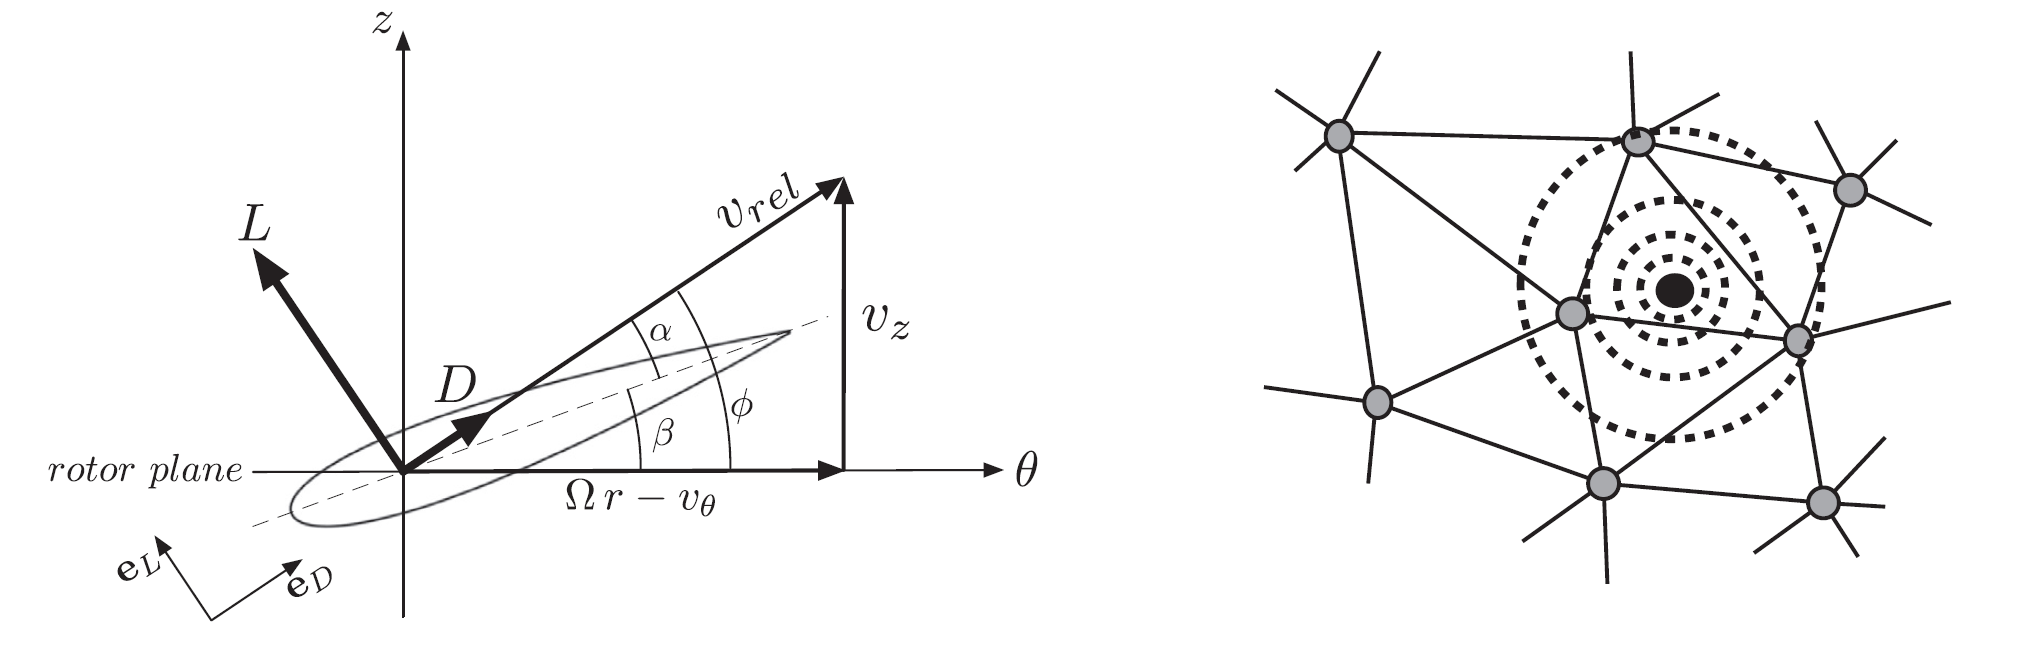
\includegraphics[scale=0.4]{./part2_developments/figures_ch4_SLI/ALM_airfoil_and_mollification_benard}
	\caption[ALM illustration of a velocity triangle and geometrical conventions in an airfoil and mollification of a point force on several nodes of an unstructured grid]{ALM illustration of a velocity triangle and geometrical conventions in an airfoil (\textsl{left}) and mollification of a point force on several nodes of an unstructured grid (\textsl{right}). Source: \citeColor[benard_large-eddy_2018].}
	\label{fig:ALM_airfoil_and_mollification_benard}
\end{figure} 
 

In the computational domain, the body forces cannot be directly applied in a single point since it would create a numerical singularity in the Navier-Stokes equations. Therefore, the body source term is applied using a mollifying function $\eta$ that distributes the body force $f$ from the forces calculated at each blade element:

\begin{equation}
\textbf{f} \left( \textbf{x}, t \right) = - \sum_{e=1}^{N} \left( L \textbf{e}_L + D \textbf{e}_D \right) \eta \left( |\textbf{r} - \textbf{r}_e| \right)
\end{equation}

where $\textbf{e}_L$ and $\textbf{e}_D$ are the unit vectors along the lift and drag directions (Figure \ref{fig:ALM_airfoil_and_mollification_benard} left), the subscript $e$ refers to each blade element and the mollifying function is defined by Eq. (\ref{eq:ch4_ALM_mollification_function}).

\begin{equation}
\label{eq:ch4_ALM_mollification_function}
\eta \left( d \right) = \frac{1}{\epsilon^3 \pi^{3/2}} \exp \left[ - \left( \frac{d}{\epsilon} \right)^2 \right]
\end{equation}

where $\epsilon = 2 w$. The mollification process is depicted in Figure \ref{fig:ALM_airfoil_and_mollification_benard} right. The simplicity of ALM and its applicability to represent the perturbations created by solid blades have seen its application to model the interaction with other bodies, such as towers in wind turbines \citeColor[benard_large-eddy_2018], and to use it for generating synthetic turbulence in the grids \citepColor[houtin-mongrolle_actuator_2020]).

%As shown in Figure (\textbf{Ref. to figure in introduction}), the dense core has a perturbation effect towards the gas phase. The resulting vortical structures will influence the dispersion of the droplets generated by atomization due to turbulent interaction. Therefore,


\subsection{Dense core representation as an actuator}

%In this work, ALM is used to model the perturbation effect of the JICF dense core on the gaseous field in dispersed phase simulations. 

As depicted in Figure \ref{fig:arienti_2006_jicf}, the presence of the dense core creates a wake and vortical structures further downstream. This interaction can be captured in resolved atomization simulations (see $\S$\ref{subsec:ch5_dense_core_in_ACLS_simus} of Chapter \ref{ch5:jicf_resolved_simulations}), but not in dispersed phase simulations where the coherent liquid structures are neglected. Since these liquid-gas interactions can have a strong influence on the transport of droplets in the developed spray region, it is of interest to model this effect in dispersed phase simulations. For this purpose, ALM is used.

\begin{figure}[h!]	
	\centering
	\includeinkscape[inkscapelatex=false,width=13cm]{./part2_developments/figures_ch4_SLI/ALM_DC_learning}
	\caption[Representation of the dense core as an actuator]{Representation of the dense core as an actuator, showing lateral (\textsl{left}) and frontal (\textsl{right}) views of the jets. \textsl{Top}: schematic dense core from a resolved simulation. \textsl{Bottom}: actuator line model of the dense core.}
	\label{fig:ALM_DC_learning}
\end{figure}

Figure \ref{fig:ALM_DC_learning} shows the representation of the dense core (top figures) as an actuator line model (bottom figures). Its complex topology is emulated by a frustum with increasing chord from the bottom ($c_0 = d_\mathrm{inj}$) to the top ($c_L = W$). The frustum has a length $L$ and an inclination angle $\theta$ which are obtained from the breakup point coordinates $(x_b, z_b)$ of the dense core in resolved atomization simulations: $L = \sqrt{x_b^2 + z_b^2}$ and $\theta = \tan^{-1} \left( z_b / x_b\right)$. The actuator points where discrete forces are placed are equally-spaced with a distance $w$ along the center line of the frustum. The number of points $N_p$ also needs to be specified in the ALM model.

Apart from the geometry, the forces applied to the actuator points are also defined. In this model, instead of specifying coefficients as done in wind turbine blades, the forces will be directly imposed in the actuator points. As shown in Figure \ref{fig:ALM_DC_learning}c, the force in the actuator will evolve linearly from the bottom to the top in order to take into account the real increasing cross-section of the actuator, which has the effect of increasing drag \citepColor[mashayek_jet_2006]. The force acts in a direction normal to the axis of the frustum. Therefore, the imposed forces can be decomposed into two components: a drag force $D$ along the $x$ direction and a lift force $L$ along the $z$ direction. Forces are specified at each actuator point with coordinates $\left( x_p, z_p \right)$ along the actuator. As the coordinates are automatically calculated according to the number of actuator points $N_p$ and the breakup point $\left( x_b, z_b \right)$, the forces will be expressed with respect to the line coordinate $s_p = \left( x_p^2 + z_p^2 \right)^{1/2}$ with expresses the distance of each actuator point to its base. Hence, the force decomposition into lift and drag holds as follows:

\begin{equation}
\textbf{F} \left( s_p \right) = D \left( s_p \right) \textbf{i} + L \left( s_p \right) \textbf{k} 
\end{equation}

where $\textbf{i}$ and $\textbf{k}$ are the unit vectors in the $x$ and $z$ directions, respectively. To estimate these forces, the net force applied to the dense core $\textbf{F}_\mathrm{DC}$ is obtained from the resolved simulations (see $\S$\ref{subsec:ch4_ALM_forces_determination}). This force is assumed to act in the same direction as the forces $\textbf{F} \left( s_p \right)$ from the actuator model, and is repartitioned into the several forces that are applied to the actuator points. Therefore, the following condition must be fulfilled:

\begin{equation}
\sum_{p=1}^{N_p} | \textbf{F} \left( s_p \right)| = | \textbf{F}_\mathrm{DC} |
\end{equation}

As the forces $| \textbf{F} \left( s_p \right)|$ increase linearly along the actuator, its evolution is represented by the following expression accordingly to the vertical coordinates $z_p$ of the actuator points:

\begin{equation}
|\textbf{F} \left( s_p \right) | = | \textbf{F}_\mathrm{DC} | \frac{s_p}{\sum_{p=1}^{N_p} s_p}
\end{equation}

And finally, the drag and lift forces to impose are calculated as follows:

\begin{subequations}
\label{eq:ALM_SLI_lift_drag_definitions}
\begin{align}
L \left( s_p \right) &= - |\textbf{F} \left( s_p \right) | \cos \theta = - | \textbf{F}_\mathrm{DC} | \cos \theta \frac{s_p}{\sum_{p=1}^{N_p} s_p} \\
D \left( s_p \right) &= |\textbf{F} \left( s_p \right) | \sin \theta = | \textbf{F}_\mathrm{DC} | \sin \theta \frac{s_p}{\sum_{p=1}^{N_p} s_p}
\end{align}
\end{subequations}

Therefore, the forces imposed to the actuator points are parametrized by the dense core net force $| \textbf{F}_\mathrm{DC} |$, the actuator inclination $\theta$ and the actuator points. Table \ref{tab:alm_parameters} shows a recap of the parameters used in the proposed model. In this table, the angle $\theta$ is not shown since it can be obtained with trigonometry from the initial and end points of the actuator. The number of actuator points $N_p$ is not taken as an input parameter as it has been checked that, if large enough, it does not have an effect of the perturbed flow field: therefore, it has been set to $N_p = 100$ for all cases presented in this thesis.

%The actuator chords shown in Figure \ref{fig:ALM_DC_learning} are not shown in this model since the increase in cross-section is directly contained in the linear evolution of the forces, Eqs. (\ref{eq:ALM_lift_drag_definitions}).

\begin{table}[!h]
\centering
\caption{Parameters of an actuator representing the dense core}
\begin{tabular}{ccc}
\thickhline
\textbf{Parameter} & \textbf{Units} & \textbf{Description} \\ 
\thickhline
$x_b, z_b$ & mm & Actuator end point  \\
%$c_0$ & mm & Chord at base of actuator \\
%$c_L$ & mm & Chord at tip of actuator \\
%$\theta$ & $\degree$ & Dense core inclination  \\
$| \textbf{F}_\mathrm{DC} |$ & N & Dense core net force\\
%$\Delta p$ & Pa & \\
\thickhline 
\end{tabular}
\label{tab:alm_parameters}
\end{table}


\subsection{Determination of forces}
\label{subsec:ch4_ALM_forces_determination}

The forces to impose in the actuator model are learnt from the resolved atomization simulation. For this purpose, the forces are firstly calculated in these simulations by calculating the corresponding term of the momentum equation (\ref{eq:momentum_conservation_general_integral}):

\begin{equation}
\boldsymbol{F}_\mathrm{DC} = \boldsymbol{F}_p + \boldsymbol{F}_\tau = \int_{\partial \Omega_{DC}} \left( \underbrace{- p \boldsymbol{n}}_{\mathrm{Pressure}} + \underbrace{2 \mu \overline{\overline{\epsilon}} \boldsymbol{n}}_{\mathrm{Shear}}  \right) dS 
\end{equation}

where $\partial \Omega_{DC}$ denotes the dense core surface. $\boldsymbol{F} $ has two contributions: a pressure force term and a shear force term. In a first instance, the shear term is neglected (see next section for details). Therefore, the total force term is reduced to the pressure force:

\begin{equation}
\label{eq:ALM_Fp_complete_integral}
\boldsymbol{F}_\mathrm{DC} = \boldsymbol{F}_p = - \int_{\partial \Omega_{DC}} p \boldsymbol{n} dS 
\end{equation}

To simplify this expression, the forces in the windward and leeward sides of the dense core are assumed to be constant as indicated in Figure \ref{fig:ALM_DC_learning}a by the red and blue arrows, respectively. The surface of the dense core can be approximated according to the actuator model as $\partial \Omega_\mathrm{DC} \approx S_\mathrm{DC} = \frac{1}{2} \left( c_0 + c_L \right) L$, being $L = \sqrt{x_\mathrm{b}^2+z_\mathrm{b}^2}$ if the actuator initial point is located at the origin of the coordinate system. Therefore, Eq. (\ref{eq:ALM_Fp_complete_integral}) can be reduced to


\begin{equation}
\label{eq:ALM_Fp_calculation_simplified}
\boxed{
|\boldsymbol{F}_\mathrm{DC}| = \left( p_\mathrm{windward} - p_\mathrm{leeward} \right) S_{DC} 
}
\end{equation}


%The approximation of considering the pressures as both sides as equal is done in this model as it has been observed in the resolved simulations (see Figure \textbf{????}), but requires further research and might be a source of error. 

It must be taken into account that the dense core as a rigid body immersed in a fluid. Its geometry has been approximated by observations of the dense core shape in resolved atomization simulations, and have been taken as constant. In reality, the dense core is a deformable body whose topology (breakup point, inclination, length) changes with time. Future works on deriving more thorough models intending to represent the dense core should take into account these transient properties \citepColor[patil_liquid_2021].

\subsubsection*{Neglecting the shear force term}

For a body immersed in a fluid, the shear force is defined as:

\begin{equation}
\boldsymbol{F}_\tau = \int_{\partial \Omega_\mathrm{DC}} 2 \mu \overline{\overline{\epsilon}} \boldsymbol{n} dS
\end{equation}

where $\overline{\overline{\epsilon}}$ is the deformation tensor:

\begin{equation}
\overline{\overline{\epsilon}} = \frac{1}{2} \left( \nabla \boldsymbol{u} + \left(\nabla \boldsymbol{u}\right)^T \right)
\end{equation}

The forces $\boldsymbol{F}_\tau$ cannot be easily calculated with the current methodology. Instead, a more simple expression of the shear forces based on a friction coefficient $C_f$ and a reference surface $S$ is used \citemColor[johnston_investigation_1984,soedarmo_simplified_2018]:

\begin{equation}
\label{eq:ALM_model_Ftau}
\boldsymbol{F}_\tau = \frac{1}{2} \rho_g u_g^2 S C_f 
\end{equation}

The friction coefficient $C_f$ is obtained from the following expression \citepColor[yang_new_2017]:

\begin{equation}
\label{eq:ALM_model_Cf}
C_f = 0.37 \left( \log Re_x \right)^{-2.584}
\end{equation}

where $Re_x$ is the Reynolds number based on the incoming velocity and the distance along the dense core.


The relative intensity of the force $\boldsymbol{F}_p$ with respect to $\boldsymbol{F}_\tau$ can be measured by dividing expressions (\ref{eq:ALM_Fp_complete_integral}) and (\ref{eq:ALM_model_Ftau}), plugging also Eq. (\ref{eq:ALM_model_Cf}):

\begin{equation}
\label{eq:rF_definition}
r_F = \frac{| \boldsymbol{F}_p| }{| \boldsymbol{F}_\tau |} = \frac{\Delta p}{0.185 \rho_g u_g^2 \left( \log Re_x \right)^{-2.584}}
\end{equation}


Where $\Delta p \sim O \left( 10^4 \right) $ in the operating points studied (see Table \ref{tab:jicf_operating_conditions} and Figure \ref{fig:JICF_turbulent_structures_planes_x} from Chapter \ref{ch5:jicf_resolved_simulations}). Considering this value, the expression for $r_F$ can be estimated to be:

\begin{equation}
r_F \sim \frac{10^5}{\rho_g u_g^2 \left( \log Re_x \right)^{-2.584}}
\end{equation}

According to the operating points studied (see Chapter \ref{ch5:jicf_resolved_simulations}), the values of $Re_x$ range from $10^3$ to $10^5$. In such points, $\rho_g = 7.21$ kg m$^{-3}$ and $u_g = 75; 100$ m s$^{-1}$. With these values, the expression of $r_F$ can be plotted as a function of $Re_x$ in Figure \ref{fig:ALM_rF_vs_Rex}. As observed, the ratio $r_F$ presents values between 10 to 90 for the $Re_x$ range of interest. These ratios mean that the pressure force $\boldsymbol{F}_p$ is between 10 and 90 times the shear force $\boldsymbol{F}_\tau$. Therefore, $|\boldsymbol{F}_\tau| << |\boldsymbol{F}_p|$ and only the contribution of the pressure force is considered to calculate the dense core net force.




\begin{figure}[h!]
	\centering
	\includegraphics[scale=0.5]{./part2_developments/figures_ch4_SLI/ALM_rF_vs_Rex.eps}
	\caption{Force ratio evolution with $Re_x$.}
	\label{fig:ALM_rF_vs_Rex}
\end{figure}


\section{Secondary atomization modeling}
\label{sec:ch4_secondary_atomization_modeling}

In disperse phase simulations, spray is modeled by a set of spherical and rigid particles whose dynamics are governed by the point-particle equations described in $\S$\ref{sec:ch3_EL_formalisms}. Due to these assumptions, particles will not break by their interaction with the gaseous phase as in the resolved atomization simulations. Nevertheless, further breakup can be taken into account by means of secondary atomization models. The most important parameter governing secondary atomization is the Weber number based on the relative velocities between liquid and gas $u_\mathrm{rel}$:

\begin{equation}
\label{eq:We_secondary_atomization_definition}
We = \frac{\rho_g u_\mathrm{rel}^2 r}{\sigma} 
\end{equation}

Different mechanisms produce secondary atomization depending on the value of We, see Fig. \ref{fig:regimes_atomization_secondary}. Existing models for secondary atomization have been developed for each particular mode of breakup, such as the WAVE model for high Weber numbers \citepColor[reitz_modeling_1987] or the Taylor Analogy Breakup (TAB) model for low ones \citepColor[orourke_tab_1987]. The former model predicts breakup by following a linear stability analysis considering Kelvin-Helmholtz waves as the governing breakup mechanisms, while the latter makes an analogy between a droplet and a second-order mechanical system. Nevertheless, up to date there is not a model which accounts for all different breakup mechanisms and that can capture all the physical complexity of secondary atomization.

In this work, three atomization models have been implemented and tested: the TAB model, the Enhanced TAB model \citepColor[tanner_liquid_1997], and the stochastic model of \citeColor[gorokhovski_stochastic_2001]. They are described in the following sections.

\subsection{Taylor Analogy Breakup}


\begin{figure}[h!]
	\centering
	\includeinkscape[inkscapelatex=false,scale=0.75]{./part2_developments/figures_ch4_SLI/TAB_analogy}
	\caption{Taylor analogy breakup between a droplet and a mechanical system with spring and damper. The undeformed droplet is represented by the dashed line, while the thick solid line depicts the droplet after deformation. $x$ is the displacement from the deformed to the undeformed states.}
	\label{fig:TAB_droplet_deformation}
\end{figure}

The Taylor Analogy Breakup (TAB) model is one the first secondary atomization models. Developed by \citeColor[orourke_tab_1987], it makes an analogy between a droplet and a mechanical system as shown in Fig. \ref{fig:TAB_droplet_deformation}. Breakup occurrence is estimated by solving the ordinary differential equation (ODE) representing the oscillating dynamics of the mechanical system depicted:

\begin{equation}
\label{eq:TAB_ODE_x}
m \ddot{x} = F - k x - c \dot{x}
\end{equation}

where $x$ is the displacement from the droplet's equator due to deformation, $m$ is the mass, $F$ is the external force, $k$ is the spring constant and $c$ is the damping coefficient. The Taylor analogy makes a comparison between this mechanical system and the droplet, producing the following relation between constants:

\begin{equation}
\frac{F}{m} = C_F \frac{\rho_g u_\mathrm{rel}^2}{\rho_l r} ~~~~ ; ~~~~ \frac{k}{m} = C_k \frac{\sigma}{\rho_l r^3} ~~~~ ; ~~~~ \frac{c}{m} = C_d \frac{\mu_l}{\mu_g r^2}
\end{equation}

where $C_F = 1/3$, $C_k = 8$, $C_d = 5$ are constants, $r$ the droplet radius, $\rho$ the density, $\sigma$ the surface tension, $\mu$ the viscosity, and the subscripts $l$ and $g$ indicate liquid and gases respectively. 

The deformation $x$ can be expressed by a non-dimensionless parameter $y$, hereafter referred as droplet distorsion, whose equivalence is $y = x / \left( C_b r \right)$, where $C_b = 0.5$ is a constant. Using the expressions from the Taylor analogy and introducing the change of variable $y$, the ODE (\ref{eq:TAB_ODE_x}) changes to:

\begin{equation}
\label{eq:TAB_ODE}
\ddot{y} = \frac{C_F}{C_b} \frac{\rho_g}{\rho_l} \frac{u_{rel}^2}{r^2} - \frac{C_k \sigma}{\rho_l r^3} y - \frac{C_d \mu_l}{\rho_l r^2} \dot{y}
\end{equation}

This expression governs the breakup of droplets, which occurs for $y > 1$ (i.e. when the amplitude of the oscillation $x$ equals the radius of the undeformed droplet). For solving this equation, it is useful to introduce the following parameters:

\begin{subequations}
\label{eq:TAB_td_omega_definition}
\begin{align}
t_d &= \frac{2 \rho_l r^2}{C_d \mu_l} \\
\omega^2 &= C_k \frac{\sigma}{\rho_l r^3} - \frac{1}{t_d^2}
\end{align}
\end{subequations}

where $t_d$ is the oscillation damping time and $\omega$ is the oscillations frequency. With these definitions, the solution to Eq. (\ref{eq:TAB_ODE}) is:

\begin{equation}
\label{eq:yTAB_equation_general}
y \left( t \right) = We_c + e^{- t / t_d} \left[ \left( y_0 - We_c \right) \cos \left( \omega t \right) + \frac{1}{\omega}\left( \dot{y}_0 + \frac{y_0 - We_c}{t_d} \right) \sin \left( \omega t \right)   \right]
\end{equation}

where $We_c = \frac{C_F}{C_k C_b} We = We / 12$ with the constants previously defined. The distorsion rate can be obtained by differentiating the former expression with time:

\begin{equation}
\label{eq:dydtTAB_equation_general}
\dot{y} \left( t \right) = \frac{We_c - y \left( t \right) }{t_d} + e^{- t / t_d} \left[ \left( \dot{y}_0 + \frac{y_0 - We_c}{t_d} \right) \cos \left( \omega t \right) - \omega \left( y_0 - We_c \right) \sin \left( \omega t \right)  \right]
\end{equation}

As it can be seen, the previous equations are continuous. For numerical implementation of the algorithm, it is more convenient to express them in their corresponding discrete form:

\begin{equation}
\label{eq:yTAB_equation_discrete}
y^{n+1} = We_c + e^{- dt / t_d} \left[ \left( y^n - We_c \right) \cos \left( \omega dt \right) + \frac{1}{\omega}\left( \dot{y}^n + \frac{y^n - We_c}{t_d} \right) \sin \left( \omega dt \right)   \right]
\end{equation}

\begin{equation}
\label{eq:dydtTAB_equation_discrete}
\dot{y}^{n+1} = \frac{We_c - y^{n+1} }{t_d} + e^{- dt / t_d} \left[ \left( \dot{y}^n + \frac{y^n - We_c}{t_d} \right) \cos \left( \omega dt \right) - \omega \left( y^n - We_c \right) \sin \left( \omega dt \right)  \right]
\end{equation}

where the subindexes $n$ and $n+1$ indicate two consecutive time instants separated by the timestep $dt$.

To estimate breakup, firstly $\omega^2$ is calculated with Eq. (\ref{eq:TAB_td_omega_definition}b). According to its value, two scenarios are possible:

\begin{itemize}

	\item If $\omega^2 < 0$, oscillations are not present. Hence, the droplet does not deform and the values for droplets distorsion and distorsion rate are set to $0$: $y^{n+1} = y^n = 0$.
	
	\item If $\omega^2 > 0$, breakup is possible. In this case, the amplitude of oscillations $A$ is calculated:
	
	\begin{equation}
	A = \sqrt{\left( y^n - We_c \right)^2 + \left( \dot{y}^n / \omega \right)^2}
	\end{equation}

\end{itemize}

Again, the value of $A$ will present two different alternatives:

\begin{itemize}

	\item If $We_c + A \leq 1$, then $y^n \leq 1$ and droplet will not break. Deformation and deformation rate will then be updated by applying Eqs. (\ref{eq:yTAB_equation_discrete}) and (\ref{eq:dydtTAB_equation_discrete}).
	
	\item If $We_c + A > 1$, breakup is possible. A breakup timestep $dt_{bu}$ is then calculated as the smallest root of the following equation:
	
	\begin{equation}
	\label{eq:TAB_dtbu_obtention}
	We_c + A \cos \left( \omega dt_{bu} + \phi  \right) = 1
	\end{equation}

\end{itemize}

where the phase $\phi$ is obtained from the following:

\begin{equation}
\cos \phi = \frac{\dot{y}^n - We_c}{A} ~~~~ ; ~~~~ \sin \phi = - \frac{\dot{y}^n}{A \omega}
\end{equation}

Breakup will then occur in the case that $dt < dt_{bu}$, or also if updating the deformation it is found that $y^{n+1} > 1$. Once breakup is triggered, the associated droplet (named parent) will divide into one or several smaller particles (named children). The mean size of children droplets $r_{32}$ is obtained through an energy balance between the produced droplets and the parent with radius $r$, yielding the following relation between both sizes:

\begin{equation}
\label{eq:TAB_model_radius_ratio}
\frac{r}{r_{32}} = 1 + \frac{8 K}{20} + \frac{\rho_l r^3}{\sigma} \dot{y}^2 \left( \frac{6 K - 5}{120} \right)
\end{equation}

where $K = 10/3$ is a constant. Now, radii of children droplets $r_{ch}$ are randomly chosen from a Rosin-Rammler distribution \footnote{In the original work by \citeColor[orourke_tab_1987], a $\chi^2$ distribution is used} with characteristic diameter $r_{32}$ and factor $q = 3.5$: 


\begin{equation}
\label{eq:rossin_rammler_distribution}
Q \left( r \right) = 1 - \exp\left(  - \left( \frac{r}{r_{0.632}} \right)^q \right)
\end{equation}

which can be inverted to obtain $r_{ch}$:

\begin{equation}
\label{eq:r_ch_TAB_family}
r_{ch} = r_{32} \sqrt[3.5]{- \log \left( 1 - Q \right) }
\end{equation}

where $Q$ is Cumulative Density Function (CDF). To estimate the size of children droplets droplets from this distribution, $Q$ is randomly sampled from a uniform distribution $\in [0,1]$. The resulting random number is introduced in the previous expression, yielding a value for one children droplet. This procedure is repeated until the volume of all children droplets equals the volume of the parent, hence conserving mass. Children droplets are then randomly located along the surface of the parent droplet. They will all inherit the velocity of the parent droplet, plus a component $v_\perp$ with magnitude:

\begin{equation}
\label{eq:TAB_v_perp}
v_\perp = C_v C_b r \dot{y}^n
\end{equation}

where $C_v \approx 1$. The direction of $v_\perp$ is randomly chosen in a plane normal to the relative velocity $u_\mathrm{rel}$. Finally, all children droplets all initialised with $y = \dot{y} = 0$.



\subsection{Enhanced TAB model}

The main disadvantage of the TAB model is the underprediction of droplets size. To overcome this problem, an improved version of the TAB model was developed by \citeColor[tanner_liquid_1997], named Enhanced Taylor-Analogy Breakup (ETAB). Breakup is predicted and triggered in the same way as in TAB, but the size of children droplet is estimated differently. While TAB makes use of an energy balance \citepColor[orourke_tab_1987], ETAB considers that the droplet production rate is proportional to the number of children droplets. Mathematically, this proportionality is expressed by the following exponential decay law:

\begin{equation}
\label{eq:ETAB_rate_production_law}
\frac{d m_\mathrm{ch}}{dt} = - 3 K_\mathrm{br} m_\mathrm{ch}
\end{equation}

where $m_\mathrm{ch}$ is the mass of children droplets. This law depends on the atomization regime through the breakup constant $K_\mathrm{br}$, which depends on $We$ and the oscillation frequency $\omega$:

\begin{equation}
\label{eq:ETAB_Kbr_equation}
K_{br} =
\left\{
    \begin{split}
    k_1 \omega \,\,\mathrm{if}\,\,We \leq We_t \\ 
    k_2 \omega \sqrt{We} \,\,\mathrm{if}\,\,We > We_t
    \end{split}
\right.
\end{equation}

where $k_1$ and $k_2$ are constants, and $We_t$ is a transition Weber number between bag and stripping breakup regimes, set to 80 \citepColor[tanner_liquid_1997]. The bag breakup $k_1$ is obtained from the following expression to make a smooth transition between both regimes:

\begin{equation}
k_1 = k_1^* \left[\left(  \frac{k_2}{k_1^*} \left( \sqrt{We_t} - 1 \right) \right) \left( \frac{We}{We_t} \right)^4 + 1 \right]
\end{equation}

where $k_1^* = 2/9$. The stripping breakup constant is fixed to $k_2 = 2/9$.

The size of children droplets is calculated by integrating the production law Eq. (\ref{eq:ETAB_rate_production_law}):

\begin{equation}
\label{eq:ETAB_model_radius_ratio}
\frac{r_{ch}}{r} = e ^{-K_{br} t_{bu}}
\end{equation}

where $t_{bu}$ is estimated as in the TAB model, Eq. (\ref{eq:TAB_dtbu_obtention}). All children droplets generated from a parent with radius $r$ will have identical size $r_{ch}$. Finally, children will inherit parent's velocity plus a normal component given by:

\begin{equation}
v_\perp = C_A C_b r \left(\dot{y}^n\right)^2 
\end{equation}

whose direction is randomly chosen in a plane normal to the relative velocity $u_\mathrm{rel}$. In this expression, $C_A$ is a constant determined from an energy balance:

\begin{equation}
C_A^2 = 3 \left( 1 - \frac{r_{ch}}{r} + \frac{5}{72} C_D We \right) \frac{\omega^2}{\dot{y}^2}
\end{equation}

being $C_D$ is the drag coefficient of the parent droplet, Eq. (\ref{eq:Re_CD_droplet}). Note that $v_\perp$ defined by the ETAB model differs from TAB's Eq. (\ref{eq:TAB_v_perp}) by considering $C_A$ to be dependent on the breakup regime.


\subsection{Gorokhovski stochastic model}
\label{subsec:ch4_goro_model}

Both TAB and ETAB models were derived using the Taylor analogy breakup. The TAB model is known \citemColor[tanner_liquid_1997,dahms_significance_2016,fontes_improved_2019] to underestimate the diameter of the children droplets and to not distinguish between breakup regimes,
producing too many droplets when the Weber number is high. Hence, the applicability of TAB is restricted to breakup at low $We$. ETAB tried to solve this issue by considering an exponential decay law for the size of children droplets which would depend on the breakup regime. Both models are, however, deterministic in the sense that a single range of droplet sizes is considered when breakup is produced.

A different secondary atomization model not based on the Taylor analogy was derived by \citeColor[gorokhovski_stochastic_2001]. This model circumvents the deterministic approach of the TAB family of models by accounting for a range of children droplet sizes when breakup occurs. This is done by using a stochastic approach based on Kolmogorov's theory of breakup \citepColor[kolmogorov_log-normal_1941]. Following this theory, the evolution of droplet's sizes is represented by a Fokker-Planck equation: 

\begin{equation}
\frac{\partial T \left( \ln r, t \right)}{\partial t} = - \nu  \langle \xi \rangle  \frac{\partial T \left( \ln r, t \right)}{\partial \left( \ln r \right)} + \frac{1}{2} \nu  \langle \xi^2 \rangle  \frac{\partial^2 T \left( \ln r, t \right)}{\partial \left( \ln r \right)^2}
\end{equation}

where $T \left( \ln r, t \right)$ is the cumulative distribution of droplets sizes, $\nu$ the breakup frequency, and  $\langle \xi \rangle$ and $ \langle \xi^2 \rangle$ are parameters. After some mathematical development \citepColor[apte_les_2003], the cumulative distribution function can be expressed as:

\begin{equation}
\label{eq:gorokhovski_T_CDF}
T \left( \ln r, t \right) = \frac{1}{2} \left( 1 + \erf \left( \frac{\ln r - \ln r_{ch} - \langle \xi \rangle }{\sqrt{2 \langle \xi^2 \rangle}}\right)  \right)
\end{equation}

This function will be later used to obtain the size of children droplets. The previous step is to determine when breakup occurs. In this model, two criteria are used:

\begin{itemize}

	\item Parent droplets must be larger than a critical radius $r_\mathrm{cr}$. This value is determined from a critical Weber number $We_\mathrm{crit} = 6$:
	
	\begin{equation}
	r_\mathrm{crit} = \frac{We_\mathrm{crit} \sigma}{\rho_g u_\mathrm{rel}^2}
	\end{equation}
	
	\item The residence time of the particles must be larger than a computed breakup time $t_\mathrm{bu}$:
	
	\begin{equation}
	t_{bu} = B \sqrt{\frac{\rho_l}{\rho_g}} \frac{r}{u_{rel}}
	\end{equation}
	
	where $B = \sqrt{3}$.

\end{itemize}

If both $r > r_\mathrm{crit}$ \textbf{and} $t > t_{bu}$, breakup occurs. In this case, size of children droplet is obtained from the cumulative density function $T \left( \ln r_{ch}, t \right)$, Eq. (\ref{eq:gorokhovski_T_CDF}), from which $\ln r_{ch}$ can be solved:
 
 
\begin{equation}
\label{eq:r_ch_goro}
r_{ch} = r \exp \left( \langle \xi \rangle  + \sqrt{2 \langle \xi^2 \rangle} \erf^{-1} \left(  2 T - 1 \right) \right)
\end{equation}

%\begin{equation}
%\ln r_{ch} = \ln r + \langle \xi \rangle  + \sqrt{2 \langle \xi^2 \rangle} \erf^{-1} \left(  2 T - 1 \right)
%\end{equation}

The size of children droplets are then obtained by sampling a random value of $T$ from a uniform distribution between $0$ and $1$, $T \sim \mathcal{U} \left( 0, 1 \right)$ , and then applying the previous equation. The parameters $\langle \xi \rangle$ and $\langle \xi^2 \rangle$ are calculated from the following equations:

\begin{subequations}
\label{eq:gorokhovski_epsilon_parameters_definition}
\begin{align}
\langle \xi \rangle &=  K_1 \ln \left(  \frac{We_c}{We}  \right) \\
- \frac{\langle \xi \rangle}{\langle \xi^2 \rangle} &=  K_2 \ln \left( \frac{r}{r_{crit}} \right)
\end{align}
\end{subequations}

where $K_1$ and $K_2$ are model constants, which are of order unity. The constant $K_1$ controls the mean size of children droplets, while $K_2$ influences its standard deviation.

Children droplets inherit then a velocity which has two components: the parent particle velocity in the same direction, plus a velocity normal to the parent's direction and magnitude equal to:

\begin{equation}
|\textbf{u}_\mathrm{ch,n} | = \frac{r}{t_{bu}}
\end{equation}




%
%\subsection{Analysis of sizes and number of children droplets}
%
%An analysis of sizes and estimated number of droplets produced by each model is done in the following lines.
%
%The estimated number of children for each model can be obtained as:
%
%\begin{equation}
%N_{ch} = \left( \frac{r}{r_{ch}} \right)^3
%\end{equation}
%
%\paragraph{Gorokhovski} Constants $K_1$, $K_2$ need to be tuned. \textbf{2009 Apte} uses the values $K_1 = 0.6$ and $K_2 = 1$ for simulating spray in a swirl injector. \textbf{Senoner PhD 2010} uses $K_1 = 0.1$, $K_2 = 0.8$ for simulating a diesel spray injected in a high-pressure chamber; and the values  $K_1 = 0.02$, $K_2 = 0.16$ for simulating a high-pressure jet in crossflow. The effect of these two constants will be investigated in our models.
%
%As done for the models from the TAB family, a mean size for children droplets can be estimated. The parameter $\xi$ from Eq. (\ref{eq:gorokhovski_T_CDF}) is defined as $\xi = \ln \left( \frac{r_{ch}}{r}  \right)$. Introducing this expression into Eq. (\ref{eq:gorokhovski_epsilon_parameters_definition}a) 
%
%\begin{equation}
%\langle \ln \left( \frac{r_{ch}}{r}  \right) \rangle = K_1  \ln \left(  \frac{We_c}{We}  \right) 
%\end{equation}
%
%By rearranging this equation we can express the mean size of children droplets:
%
%\begin{equation}
%\langle  \frac{r_{ch}}{r} \rangle = \left( \frac{We_c}{We} \right)^{K_1}
%\end{equation}
%
%This equation confirms the previous statement that the constant $K_1$ has a direct influence on the size of children droplet generated: the larger $K_1$ is, the smaller children droplets are (since the ratio $We_c/We < 1$). Generated children droplet can still undergo further breakup if they meet the breakup conditions (cascade effect), so decreasing $K_1$ would a priori limit the size of droplets (and hence their number) only in each iteration. Nevertheless, this can suppose a smooth transition of breakup towards equilibrium, which would ensure that the Weber number of children droplets is closer to its critical value (i.e. the limit of breakup). An aggressive breakup, which could be produced with a low value of $K_1$, could generate many children droplets from a parent particle with very small size that would not be found in reality (see Figures \ref{fig:r_ratio_gorok} and \ref{fig:N_ch_gorok}).
%
%
%
%\begin{figure}[h!]
%	\centering
%	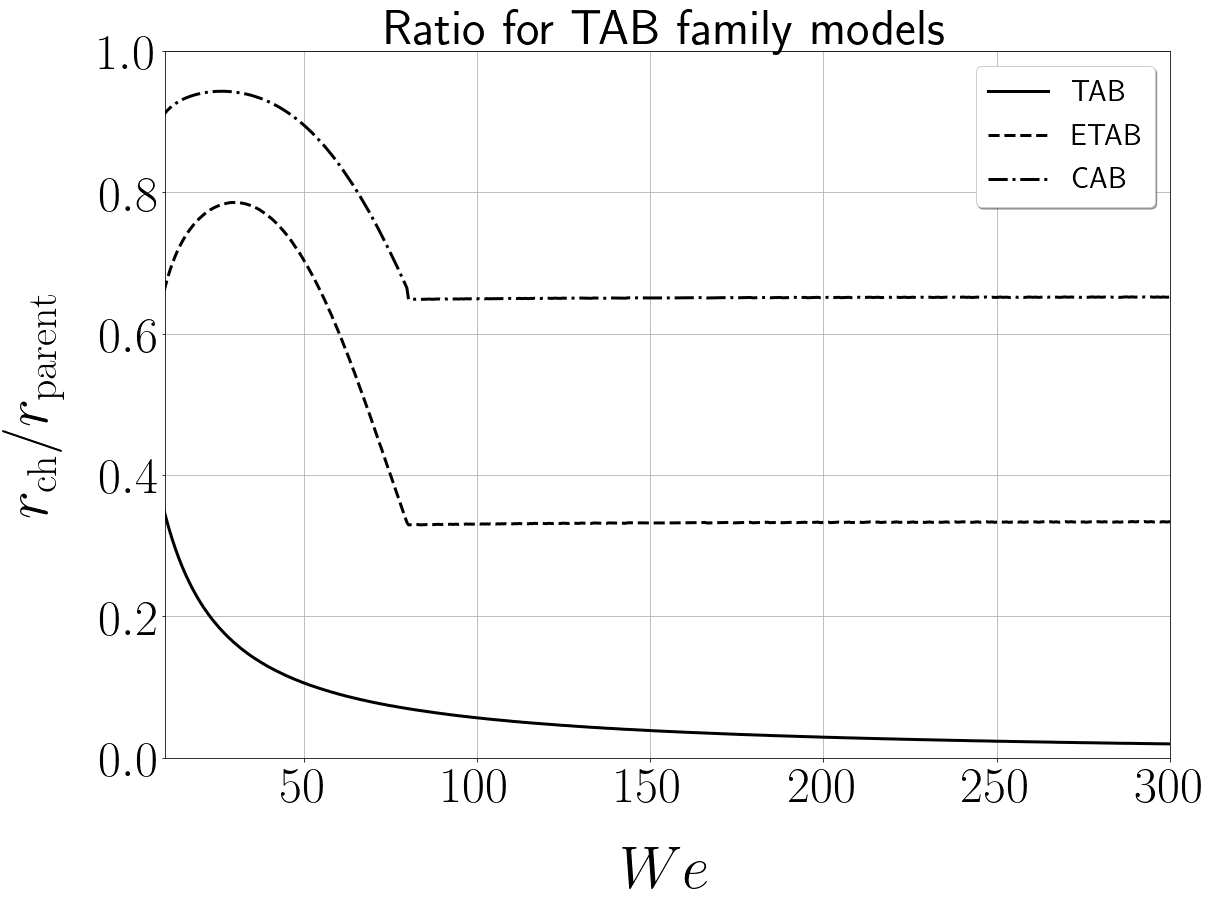
\includegraphics[scale=0.2]{./part2_developments/figures_ch4_SLI/ratio_droplet_size_TAB}
%	\caption{Ratio of mean droplet for TAB family of models}
%	\label{fig:r_ratio_TAB}
%\end{figure}
%
%\begin{figure}[h!]
%	\centering
%	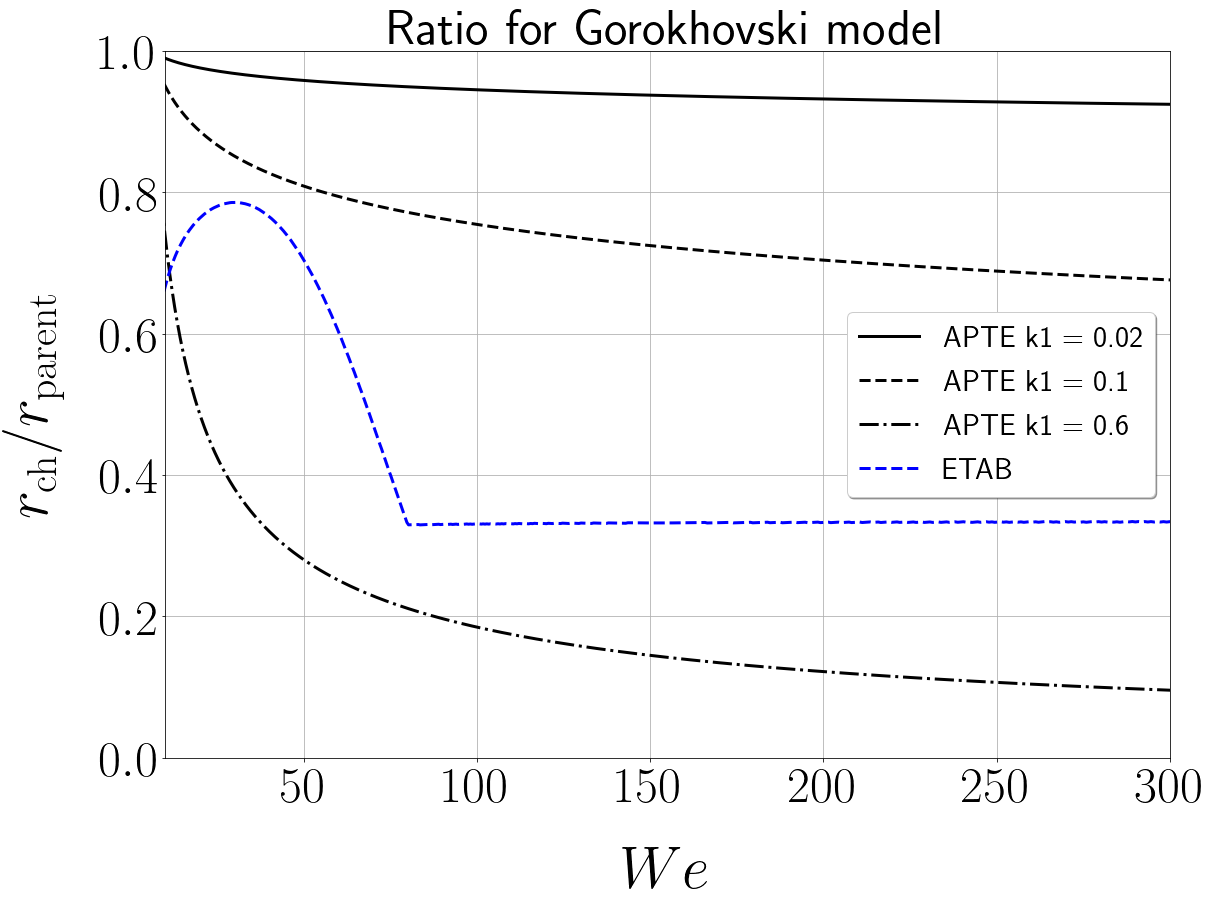
\includegraphics[scale=0.2]{./part2_developments/figures_ch4_SLI/ratio_droplet_size_gorok}
%	\caption{Ratio of mean droplet for Gorokhovski model}
%	\label{fig:r_ratio_gorok}
%\end{figure}
%
%\begin{figure}[h!]
%	\centering
%	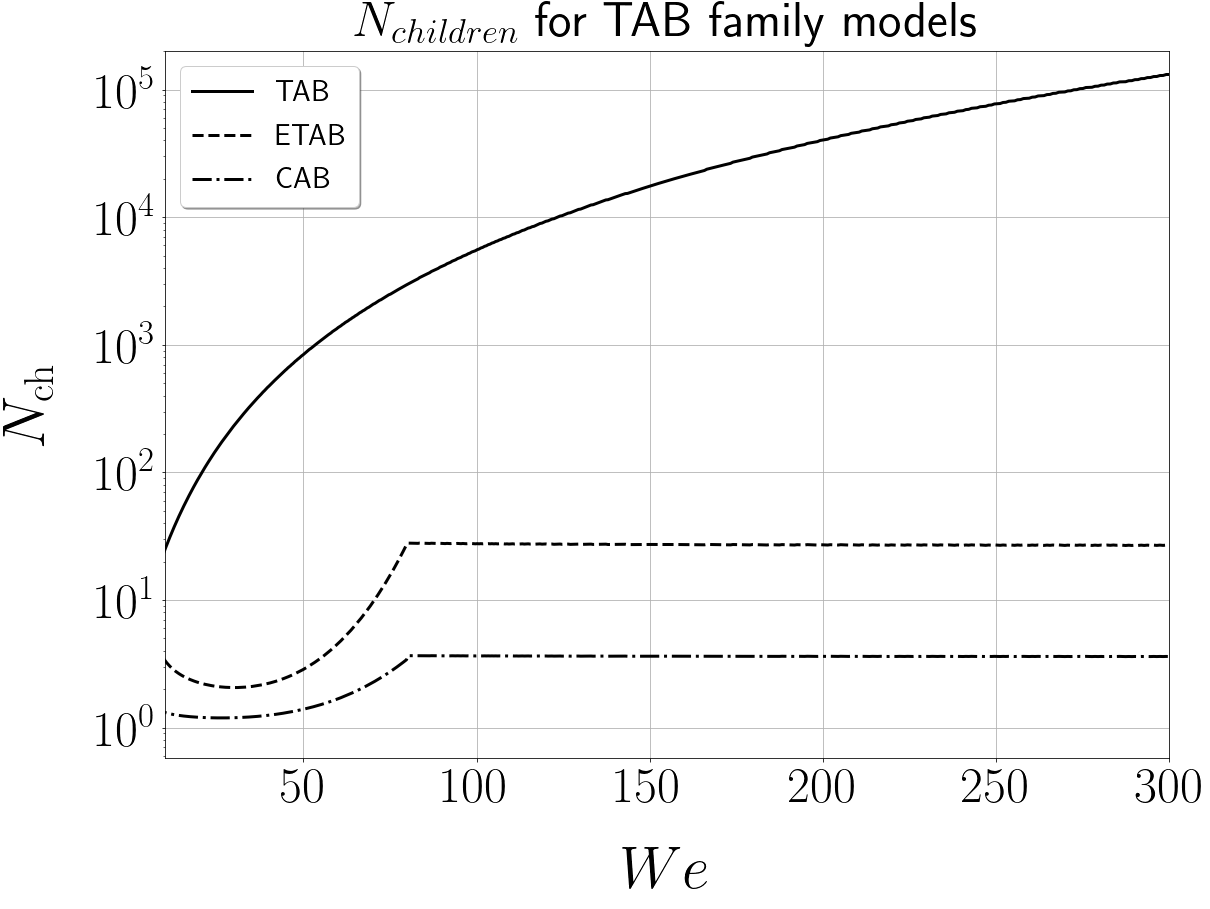
\includegraphics[scale=0.2]{./part2_developments/figures_ch4_SLI/N_ch_TAB}
%	\caption{Estimated number of children for TAB family of models}
%	\label{fig:N_ch_TAB}
%\end{figure}
%
%\begin{figure}[h!]
%	\centering
%	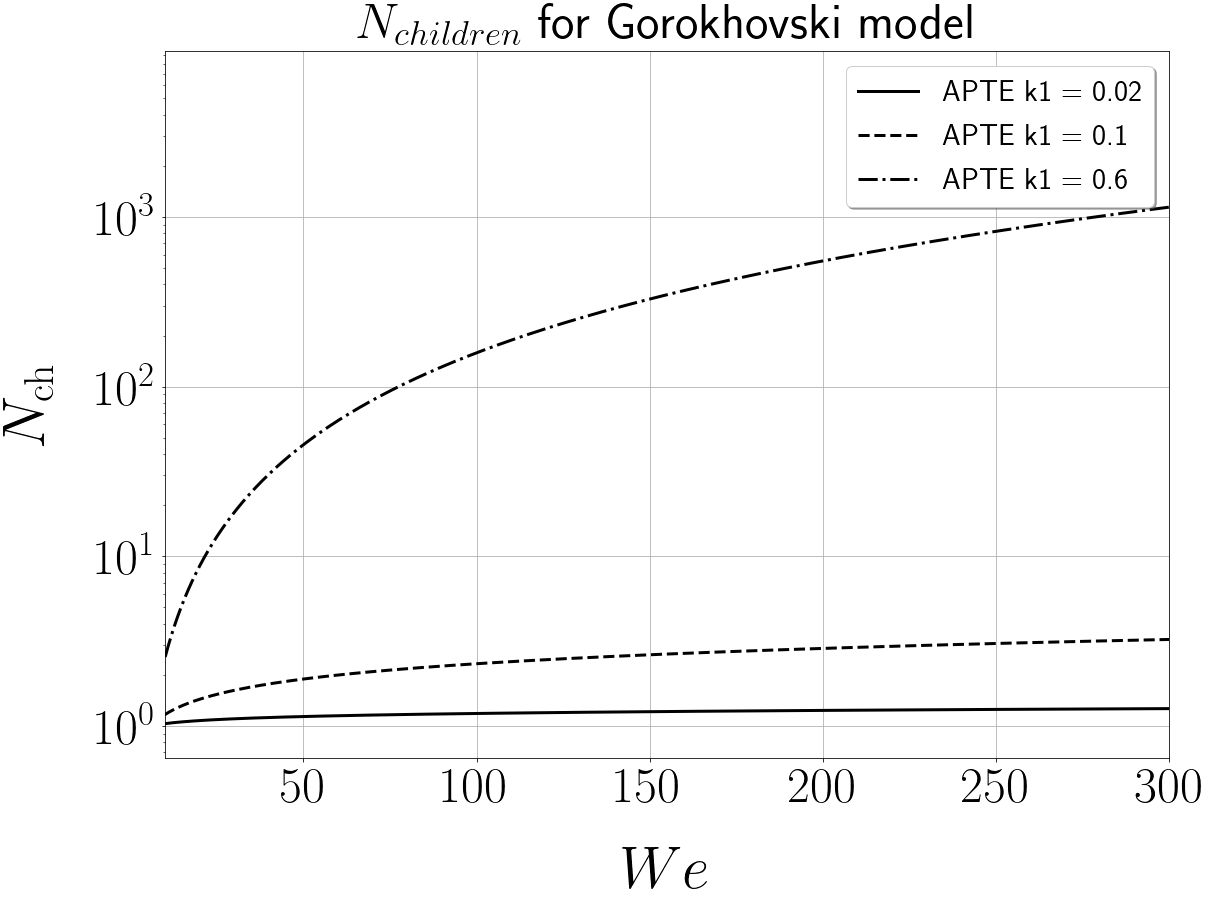
\includegraphics[scale=0.2]{./part2_developments/figures_ch4_SLI/N_ch_gorok}
%	\caption{Estimated number of children for Gorokhovski model}
%	\label{fig:N_ch_gorok}
%\end{figure}



%\section{Subgrid models for turbulent dispersion}
%
%\subsubsection*{Review}
%
%Regarding turbulent dispersion models, there are the ones used in RANS studies:
%
%\begin{itemize}
%
%	\item \textbf{2016 Eckel} mentions two dispersion models: Gosmann and Ioannides (the classic) (1983), (Blumcke et al. 1993)
%	
%	\item \textbf{Fontes 2018} uses the Langevin dispersion model introduced in Sommerfeld 2001
%
%	\item \textbf{Belmar 2020} presents a turbulent dispersion model by O'Rourke.
%
%\end{itemize}
%
%For LES, Iafrate 2016 shows a good modelling of turbulent dispersion applied to gasoline injection ($\S$8.2 Impact de la turbulence sous-maille), based on references 120-124.
%
%Also, references I have for LES are 2015 Minier, Minier ref. 57, 2014 Urzay - Particle-laden flows.
%
%A nice one is the techical report Amsden 1989 - KIVA II.
%
%OJO: reference OKongo and Bellan de Minier ref. 57 puede ser fundamental, hace analisis de particulas con distintas velocidades inyectadas !!


\section{Conclusions and perspectives}

This chapter has introduced and detailed the injection models developed in the works of this thesis. The full process is depicted by the flowchart of Figure \ref{fig:SLI_graphic_description}. The learning of the liquid injectors, baptised as SLI, is based on a spray characterization process of droplets resulting from resolved atomization simulations. Such process consists of sampling a flux-density distribution of droplets and evaluating its convergence to then make an in-plane discretization of the spray. Then, the individual sprays of the discrete grid are characterized by average values of fluxes, diameters, and velocities, and by RMS values of velocities. The spray grid can also be further refined through a convergence-driven discretization process. Then, resulting injectors can be used to inject a realistic spray in dispersed phase simulations. The models are then closed by including in the dispersed phase simulations: 1) a modelisation of the dense core perturbance effect with ALM, which is based on a learning process from the resolved atomization simulations; and 2) a secondary atomization model that continues breaking the particles in case they are not in equilibrium with the surrounding air. The next chapters are devoted to the two-phase simulations and the application of the models. \\

For further development of the models, the following perspectives could be considered:

\begin{itemize}

	\item Include a modified drag coefficient for lagrangian particles which depends on the deformation of the liquid structures sampled in resolved atomization simulations. This would allow for a more accurate transport of the lagrangian spray at the first time instants of injection, which would affect the particle's trajectories and the liquid-gas relative velocity before secondary breakup takes place. 
	
	\item Consider a transient spray obtained through the accumulation process to develop an unsteady injection model. This would be specially useful in reactive cases where thermoacoustic oscillations play an important role, such as gas turbine and rocket engines. 

	\item Extend the spray convergence criterion, defined as a MSE norm on the droplet diameters, to include other parameters such as liquid velocities.
	
	\item Improve the actuator line model developed in this thesis to make a better representation of the resolved dense core, such as by considering a transient behaviour of its topology and its force.

\end{itemize}
\newpage 
\chapter{Learning data from a resolved liquid jet in crossflow}
	\label{ch5:jicf_resolved_simulations}



Describe here all our simulations done with JICF, what we have achieved with them, etc.

\begin{itemize}

	\item Experimental setup description
	
	\item Numerical setup description. Operating points
	
	\item Mesh convergence study
	
	\item Spray sampling
	
	\item Direct measurement of fluxes with interior boundaries
	
	\item Liquid disappearing (set levelset band ) ??
	
	\item Results:
	
		\begin{itemize}
		
			\item Breakup mechanisms
			
			\item In-nozzle phenomena of flow separation (and entrainment of gaseous bubbles)
			
			\item Spray formation and evolution with axial distance
	
		\end{itemize}
		
	\item Other results:
	
		\begin{itemize}
		
			\item Slip velocity evolution
			
			\item Vorticity distribution (horse-shoe vortices, double vortical structural in liquid)
		
		\end{itemize}

\end{itemize}

\newpage 

\section{Introduction}

The previous chapter has detailed the theory of the proposed models to build lagrangian injectors for initialising dispersed phase simulations, named Smart Lagrangian Injectors (SLI). These models, nowadays in its earliest state of maturity, are intended to be generic and applicable to a broad range of operating conditions and injector configurations. To show its capabilities, they have been developed in their first stage with resolved simulations of liquid jet in crossflow (JICF) configuration. This chapter details these simulations, performed with the software YALES2 \citepColor[moureau_design_2011]. % \textbf{https://reader.elsevier.com/reader/sd/pii/S1631072110002111?token=9137B6903478D4E8E427F5D8218DFC3EB42446DB034970B14BA9DE87AA7E80D130124A7EF8D8608D21D5D465CCE05A4F&originRegion=eu-west-1&originCreation=20210524114835}

The fundamentals and the physics of non-reactive JICF have been introduced in $\S$\ref{sec:ch1_fuel_injection_technology}. This chapter shows the results, analysis and injectors obtained from a kerosene JICF simulation replicating the experimental facility tested by \citeColor[becker_breakup_2002]. This configuration is used for validating the models. Section \ref{sec:ch5_experimental_bench} displays the experimental test bench, whose numerical setup and operating conditions chosen for numerical computations are detailed in Section \ref{sec:computational_setup}.


\section{Experimental test case}
	\label{sec:ch5_experimental_bench}

The experimental configuration tested by \citeColor[becker_breakup_2002] is shown in Figure \ref{fig:experiment_JICF_DLR}. The test rig is shown at the left. Liquid kerosene is injected through the atomizer ports to a quartz glass duct of rectangular cross section $25$x$40$ mm$^2$. The duct inlet is located at $120$ mm upstream the injection port. The boundary layer thickness developing along the bottom of the duct has been measured experimentally just upstream the atomizer, being between $4$ and $5$ mm. The lateral walls allow for optical access from the atomizer port until a location at 100 mm downstream. Air is introduced through two separate channels, a main one and a supplementary one. The main airflow is injected at the inlet of the quartz duct, while the supplementary one passes around it. Both airflows merge at the end of the duct and leave the domain through a common exit acting as a sonic throttle. The velocity inside the quartz can then be tuned by varying the size of the nozzle and the supplementary air flow rate. In the experiments performed, the range of air velocities goes from $u_g = 50$ to 100 m/s and the range of pressure from $p$ = 1.5 to 15 bar, hence allowing the study high-pressure conditions. The air temperature is maintained to $T_g = 290$ K. The fuel tested was kerosene Jet A-1 with density $\rho_l = 795$ kg m$^{-3}$ and surface tension $\sigma = 22 \cdot 10^{-3}$ N m$^{-1}$.

The liquid injection nozzle can be seen in Figure \ref{fig:experiment_JICF_DLR} right. It consists of a plain jet nozzle of $d_\mathrm{inj} =  0.45$ mm diameter and $L/d_\mathrm{inj}$ ratio of 1.56 with sharp edges. The average discharge coefficient for the mass flow rates of interest in the experimental studies is $0.6$. More details on the test rig can be found in \citeColor[brandt_experimental_1997].

\begin{figure}[h!]
	\centering
	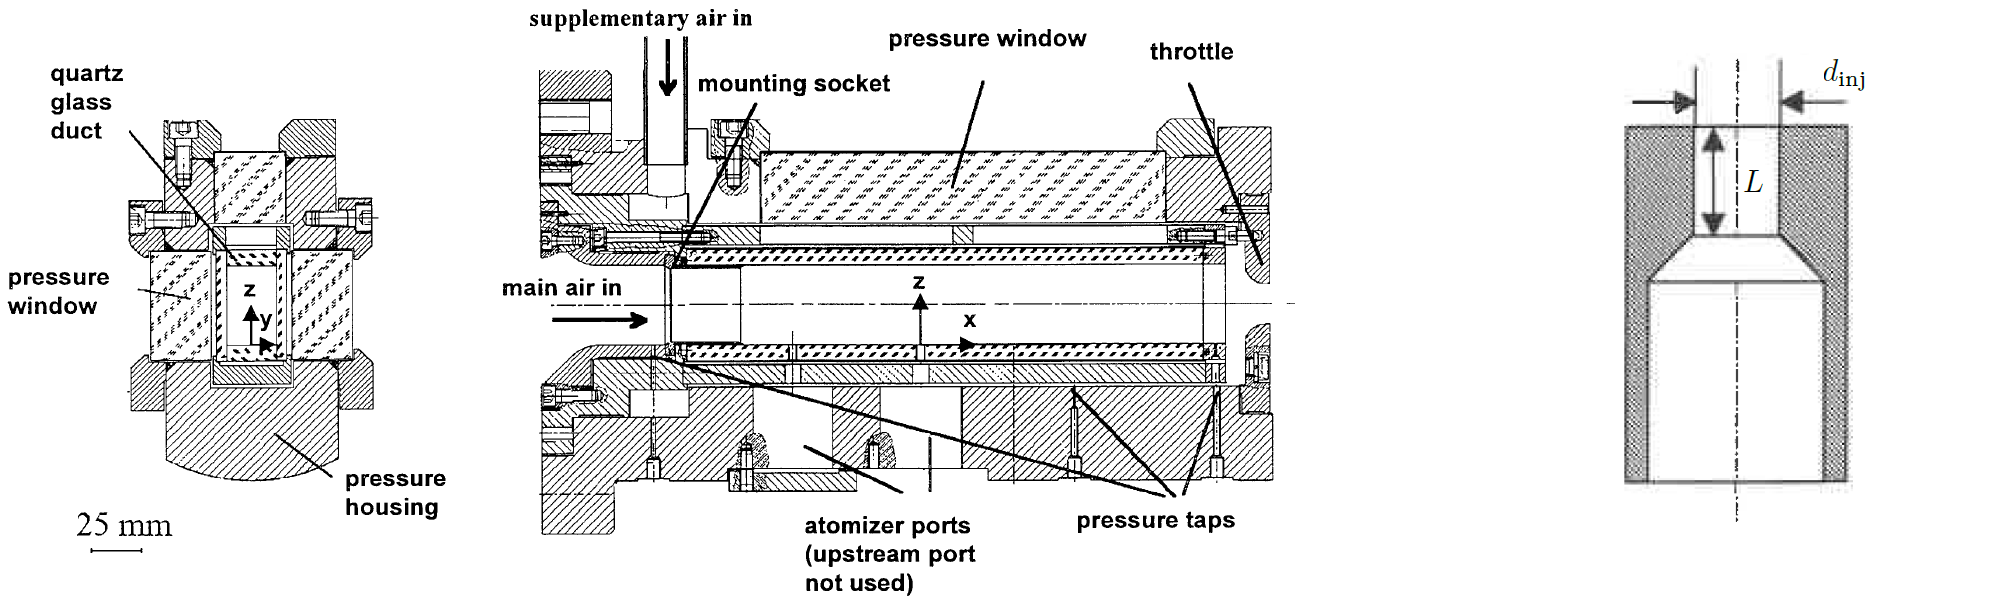
\includegraphics[scale=0.35]{./part2_developments/figures_ch5_resolved_JICF/experiment_JICF_DLR}
	\caption[JICF experimental setup]{JICF experimental setup. \textsl{Left}: Test rig. \textsl{Right}: liquid nozzle geometry employed in the experimental study. Source: \citeColor[becker_breakup_2002]}
	\label{fig:experiment_JICF_DLR}
\end{figure}


A correlation for the trajectory of the jet was obtained experimentally by analysing optically its penetration for the several operating conditions tested. It corresponds to the trajectory of the jet's windward side, and gives a relation between the vertical location $z$ with respect to the axial coordinate $z$ as a function of the nozzle diameter $d_\mathrm{inj}$ and the momentum ratio $q$ defined by Eq. (\ref{eq:q_and_We_JICF_parameters}): % The rorrelation has a standard deviation of 0.81.

\begin{equation}
    \label{eq:jicf_trajectory_becker}
    \frac{z}{d_\mathrm{inj}} = 1.57 \mathrm{q}^{0.36} \ln \left( 1 + 3.81 \frac{x}{d_\mathrm{inj}} \right)
\end{equation}



\section{Computational setup}
	\label{sec:computational_setup}

%\subsection*{Numerical domain and baseline mesh}

Figure \ref{fig:numerical_setup_maquette_JICF_DLR} shows the computational domain developed to replicate the simulations of the test bench shown in Figure \ref{fig:experiment_JICF_DLR}. The duct is modelled as a plenum consisting of a box of dimensions 25x40x270 mm$^3$. The hydraulic diameter of the duct cross section, which is used to calculate the gas Reynolds number, is $D_h = 30.8$ mm. A magnified view of the nozzle is also shown, with diameter $0.45$ mm and straight section length of 0.7 mm prior to injection to keep $L/D = 1.56$ as in the experiments. The boundary conditions are also indicated. The plenum walls use a wall law of logarithmic type except closer to the domain pressure outlet, which have been set to slip walls to avoid backflow. The nozzle walls are rigid walls. For the liquid inlet, a Poiseuille profile has been specified, while in the gaseous inlet a mean velocity profile has been set in order to recover the boundary layer thickness of between 4 and 5 mm upstream the injection nozzle as described in the experiments (see Appendix \ref{app:JICF_BL_setup} for details). Due to the high Reynolds number at the gaseous inlet (see Table \ref{tab:jicf_operating_conditions}), synthetic turbulence is added in the liquid inlet (details given in $\S$\ref{sec:ch5_initial_conditions}).

\begin{figure}[ht]
     \centering
     \includeinkscape[scale=0.35]{./part2_developments/figures_ch5_resolved_JICF/DLR_becker_numerical_config}
      \caption{Numerical domain and boundary conditions of the experimental test bench of \citeColor[becker_breakup_2002]. \textsl{Left}: complete domain. \textsl{Right}: detailed view of the injection nozzle. All dimensions are in mm.}
      \label{fig:numerical_setup_maquette_JICF_DLR}
\end{figure}

Figure \ref{fig:jicf_dlr_mesh} shows the baseline mesh, where the symmetry plane at $y = 0$ is displayed. It is composed of 66 million tetrahedral cells. The baseline cell size in the channel upstream liquid injection is 0.5 mm, while the cells located in the downstream region have an average size of 3 mm. The element size at the near-field region is 0.7 mm, and within the discharge section of the liquid nozzle it is refined to to $20 \mu m$. The justification of this mesh is done at $\S$\ref{sec:ch5_initial_conditions}, where a mesh independence study of the gaseous field is carried out. This mesh is used at the beginning of all the simulations performed, but then it change dynamically in each simulation as more liquid is introduced in the domain due to the AMR routine that refines the mesh at the liquid-gas interface ($\S$\ref{sec:YALES2}). Simulations are performed with the ACLS methodology describe in $\S$\ref{subsec:ch2_ACLS}.

\begin{figure}[h!]
	\centering
	\includeinkscape[inkscapelatex=false,scale=0.7]{./part2_developments/figures_ch5_resolved_JICF/jicf_mesh/jicf_mesh}
	\caption[Baseline JICF mesh, showing magnified views of the near-field and nozzle regions.]{Baseline JICF mesh, showing magnified views of the near-field and nozzle regions. The red rectangle is the region where meshes are shown in the mesh convergence study of $\S$\ref{sec:ch5_initial_conditions}}
	\label{fig:jicf_dlr_mesh}
\end{figure}



\section{Operating conditions}

Two operating conditions tested experimentally in \citeColor[becker_breakup_2002] have been simulated. Both of them have the same momentum ration $q = 6$ but differ in the Weber number: $We_g = 830$ (low Weber) and $We_g = 1470$ (low Weber). According to the values of $q$ and $We_g$, the former condition corresponds to surface breakup dominating regime while the latter is located at the dividing line between column and surface breakup. Figure \ref{fig:location_JICF_ops_in_breakup_map} shows the location of both operating points in the breakup map of \citeColor[wu_breakup_1997]. The physical magnitudes and dimensionless numbers of both operating points are shown in Table \ref{tab:jicf_operating_conditions}. Apart from the values $q$ and $We_g$, the dimensionless numbers in  Eq. (\ref{eq:dimensionless_numbers_jicf}) are also calculated: the liquid and gaseous Reynolds numbers $Re_g$ and $Re_g$ respectively, Ohnesorge number $Oh$, aerodynamic Weber $We_\mathrm{aero}$, relative Weber $We_\mathrm{rel}$ and density ratio $r$. These numbers have been added since they are defined in several experimental studies \citeColor[wu_breakup_1997,becker_breakup_2002,ragucci_trajectory_2007] to characterize the operating points tested. 

For performing the computations of resolved atomization, the ACLS methodology combined with the AMR routine described in $\S$\ref{subsec:ch2_ACLS} is used. For each simulation, two interface mesh sizes have been simulated: $\Delta x_\mathrm{min} = 20 ~\mu m$ (coarse case) and $\Delta x_\mathrm{min} = 10 ~\mu m$ (fine case). Therefore, a total of four simulations have been done. The nomenclature for each simulation, which is used hereafter in this document, is introduced in Table \ref{tab:jicf_resolved_simulations_performed}.

%\begin{subequations}
%\label{eq:dimensionless_numbers_jicf}
%\begin{align}
%Re_l &= \frac{\rho_l u_l d_\mathrm{inj}}{\mu_l}\\
%Re_g &= \frac{\rho_g u_g D_h}{\mu_g}\\
%We_\mathrm{aero} &= \frac{\rho_g u_l^2 d_\mathrm{inj}}{\sigma}  \\
%We_\mathrm{rel} &= \frac{\rho_g \left( u_g - u_l \right)^2 d_\mathrm{inj}}{\sigma} \\
%Oh &=  \frac{\mu_l}{\sqrt{\rho_l \sigma d_\mathrm{inj}}}\\
%r &= \frac{\rho_l}{\rho_g} 
%\end{align}
%\end{subequations}

%\begin{align}
%\label{eq:dimensionless_numbers_jicf}
%Re_l &= \frac{\rho_l u_l d_\mathrm{inj}}{\mu_l}          &  Re_g &= \frac{\rho_g u_g D_h}{\mu_g}              &  Oh &=  \frac{\mu_l}{\sqrt{\rho_l \sigma d_\mathrm{inj}}}\\
%We_\mathrm{aero} &= \frac{\rho_g u_l^2 d_\mathrm{inj}}{\sigma}    &  We_\mathrm{rel} &= \frac{\rho_g \left( u_g - u_l \right)^2 d_\mathrm{inj}}{\sigma}          & r &= \frac{\rho_l}{\rho_g} 
%\end{align}


\begin{equation}
\label{eq:dimensionless_numbers_jicf}
\begin{aligned}
Re_l &= \frac{\rho_l u_l d_\mathrm{inj}}{\mu_l}          &  Re_g &= \frac{\rho_g u_g D_h}{\mu_g}              &  Oh &=  \frac{\mu_l}{\sqrt{\rho_l \sigma d_\mathrm{inj}}}\\
We_\mathrm{aero} &= \frac{\rho_g u_l^2 d_\mathrm{inj}}{\sigma}    &  We_\mathrm{rel} &= \frac{\rho_g \left( u_g - u_l \right)^2 d_\mathrm{inj}}{\sigma}          & r &= \frac{\rho_l}{\rho_g} 
\end{aligned}
\end{equation}

\begin{table}[!h]
\centering
\caption{JICF operating points studied}
\begin{tabular}{lcccc}
\thickhline
\textbf{Parameter} & \textbf{Symbol} & \textbf{Units} &  \textbf{Low Weber} &  \textbf{High Weber} \\ %\textbf{WE\_880} &  \textbf{WE\_1470} \\
\thickhline
Nozzle diameter & $d_\mathrm{inj}$ & mm & 0.45 & 0.45 \\
%\hline
Gas bulk velocity & $u_g$ & m s$^{-1}$ & 75 & 100 \\
%\hline
Gas flow rate & $Q_g$ & m$^3$ s$^{-1}$ & 0.075  & 0.1 \\
%\hline
Liquid bulk velocity & $u_l$ & m s$^{-1}$ & 17.5  & 23.33 \\
%\hline
Liquid flow rate & $Q_l$ & mm$^3$ s$^{-1}$ & 2783  & 3710 \\
%\hline
Ambient pressure & $p_\mathrm{amb}$ & bar &  6 & 6 \\
%\hline
Gas temperature & $T_g$ & K & 290 & 290 \\
%\hline
Liquid temperature & $T_l$ & K & 288 & 288 \\
%\hline
Gas density & $\rho_g$ & kg m$^{-3}$ &  7.21 & 7.21 \\
%\hline
Liquid density & $\rho_l$ & kg m$^{-3}$ &  795 & 795  \\
%\hline
Gas viscosity & $\mu_g$ & kg m$^{-1}$ s$^{-1}$ & $1.8162 \cdot 10^{-5}$ &  $1.8162 \cdot 10^{-5}$  \\
%\hline
Liquid viscosity & $\mu_l$ & kg m$^{-1}$ s$^{-1}$ & $1.5 \cdot 10^{-3}$ & $1.5 \cdot 10^{-3}$  \\
%\hline
Surface tension & $\sigma$ & kg s$^{-2}$ &  0.022 & 0.022  \\
\thickhline
Momentum ratio & $q$ & - & 6 & 6 \\
%\hline
Gas Reynolds number & $Re_g$ & - & $0.92 \cdot 10^6$ & $1.22 \cdot 10^6$ \\
%\hline
Liquid Reynolds number & $Re_l$ & - & 4170 & 5560 \\
%\hline
Gas Weber number & $We_g$ & - & 830 & 1470 \\
%\hline
Liquid Weber number & $We_l$ & - & 5000 & 8850 \\
%\hline
Relative Weber number & $We_\mathrm{rel}$ & - & 490 & 870 \\
%\hline
Aerodynamic Weber number & $We_\mathrm{aero}$ & - & 45 & 80 \\
%\hline
Ohnesorge number & $Oh $ & - & 0.017 & 0.017 \\
%\hline
Density ratio & $r$ & - & 110 & 110 \\
%\hline
%Viscosity ratio & $\mu_l/\mu_g$ & [-] &  \multicolumn{2}{|c|}{1} \\
\thickhline
\end{tabular}
\label{tab:jicf_operating_conditions}
\end{table}

\clearpage


\begin{table}[!h]
\centering
\caption{Nomenclature for resolved atomization simulations}
\begin{tabular}{ccc}
\thickhline
%$\pmb{\Delta} x_\mathrm{min}$ [$\pmb{\mu}$$\textbf{m}])  &  \multicolumn{2}{c}{\textbf{Operating condition}} \\ 
$\Delta x_\mathrm{min}$ [$\mu$m]  &  \multicolumn{2}{c}{\textbf{Operating condition}} \\ 
\cline{2-3}
 &  Low $We_g$ &  High $We_g$ \\ 
\thickhline
\textbf{10} & UG75\_DX10 & UG100\_DX10 \\
\textbf{20} & UG75\_DX20 & UG100\_DX20 \\
\thickhline
\end{tabular}
\label{tab:jicf_resolved_simulations_performed}
\end{table}

\begin{figure}[ht]
     \centering
     \includeinkscape[inkscapelatex=false,scale=0.6]{./part2_developments/figures_ch5_resolved_JICF/jicf_breakup_regime_our_operating_points}
     \caption{Location of simulated operating conditions in the breakup map by \citeColor[wu_breakup_1997]}
	% See: https://stackoverflow.com/questions/35210337/can-i-plot-several-histograms-in-3d/35225919
      \label{fig:location_JICF_ops_in_breakup_map}
\end{figure}



%\section{YALES2 code (??)}

\section{Tools and methodologies}

%\subsection{Spray sampling in resolved simulations}

\subsection{Numerical computation of jet trajectory}
	\label{sec:ch5_tools_jicf_trajectories}

One of the most important characteristics of a jet in crossflow is its trajectory (see $\S$\ref{sec:ch1_fuel_injection_technology}). This feature determines how far the jet penetrates in the domain and has a paramount effect on the latter evaporation and mixing processes, hence affecting the flame dynamics. Experimental studies often provide correlations for the trajectory of the windward side of the jet (see Table \ref{tab:correlations_experimental_JICF}), such as the one from Eq. (\ref{eq:jicf_trajectory_becker}). These correlations depend generally on the momentum flux ratio $q$, the injection diameter $d_\mathrm{inj}$ and, in some case \citepColor[ragucci_trajectory_2007], in the Weber number $We$. The overall dependency of the trajectory on these parameters is still unknown.

Experimentally, researches have used different approaches to obtain trajectories based on the different optical techniques employed. Many works \citemColor[becker_breakup_2002,stenzler_penetration_2003,freitag_spray_2008] obtain instantaneous images of the jet with shadowgraphy techniques and then MIE scattering or emboss-filter operations to obtain binary images where liquid and gas phases can be clearly distinguished. Then, images are averaged and the vertical penetration is obtained by detecting the coordinates where the light intensity gradients are maximum. The image averaging can be performed before or after the filtering operations. These methods, which are based on obtaining the trajectories from mean images, are hereafter denoted as \textbf{mean trajectory methods}. Figure \ref{fig:expe_obtention_of_trajectories} shows an illustration of such experimental methodology from the work by \citeColor[stenzler_penetration_2003]. The filtering operations and way to obtain the light gradients vary among authors. Other works \citepColor[ragucci_trajectory_2007] use the same principles of filtering and binarization, but obtain the trajectories from instantaneous jet images. Then, the instantaneous trajectories are averaged to yield the mean trajectories. These methods are hereafter denoted as \textbf{instantaneous trajectory methods}.

From a computational perspective, similar methodologies can be applied to obtain the jet trajectories from simulations. The same sequence of operations as shown in Figure \ref{fig:expe_obtention_of_trajectories} used to process experimental images could be applied to numerical snapshots of the JICF. Nevertheless, the ACLS methodology presents the advantage that the interface can be clearly defined with the $\psi$ function, and hence it can be used to obtain the trajectory by different methods. In this work, four methodologies to obtain the numerical trajectories from JICF resolved simulations are presented. As in the experimental classification previously suggested to obtain trajectories, these methodologies are also distinguished as \textbf{mean trajectory methods} or \textbf{instantaneous trajectory methods}, depending on whether they use the mean or instantaneous $\psi$ field respectively. Two methods for each category are detailed in this section, while the results obtained are shown in $\S$\ref{subsec:ch5_jet_trajectories_results}.

\begin{figure}[ht]
     \centering
     \includeinkscape[inkscapelatex=false,scale=0.6]{./part2_developments/figures_ch5_resolved_JICF/trajectories_obtention/expe_obtention}
     \caption{Illustration of experimental procedure to obtain trajectories. Figures taken from \citeColor[stenzler_penetration_2003]}
      \label{fig:expe_obtention_of_trajectories}
\end{figure}


\subsubsection{Instantaneous trajectory methods}

The averaged numerical trajectories can be obtained from instantaneous solutions of the jet by obtaining the instantaneous trajectories for every solution obtained and then averaging them. Figure \ref{fig:trajectory_obtention_instantaneous_general} shows the procedure to extract the interface contour that is later used to obtain the trajectories. First, the liquid-gas interface is plotted in the domain as a surface of iso-contour $\Gamma: \psi = 0.5$ (Figure \ref{fig:trajectory_obtention_instantaneous_general} left), and then this contour is extracted at the central plane $y = 0$, as indicated by the black line of Figure \ref{fig:trajectory_obtention_instantaneous_general} right. 

\begin{figure}[ht]
     \centering
     \begin{subfigure}[b]{0.45\textwidth}
         \centering
         \includeinkscape[inkscapelatex=false,scale=0.35]{./part2_developments/figures_ch5_resolved_JICF/trajectories_obtention/instantaneous_interface_3D}
         %\caption{Instantaneous jet interface}
     \end{subfigure}
     %\hfill
     \begin{subfigure}[b]{0.45\textwidth}
         \centering
         \includeinkscape[inkscapelatex=false,scale=0.35]{./part2_developments/figures_ch5_resolved_JICF/trajectories_obtention/instantaneous_interface_y0}
         %\caption{Contour of instantaneous interface at plane y = 0}
     \end{subfigure}
        \caption[Procedure to obtain instantaneous trajectories.]{Procedure to obtain instantaneous trajectories. \textsl{Left}: instantaneous jet interface. \textsl{Right}: contour of instantaneous interface at plane y = 0}
	% See: https://stackoverflow.com/questions/35210337/can-i-plot-several-histograms-in-3d/35225919
        \label{fig:trajectory_obtention_instantaneous_general}
\end{figure}

Once the interface is obtained at $y = 0$, the outer contour of the trajectory must be obtained. This is the one corresponding to the windward side of the jet, and hence the one defining the instantaneous trajectory. For its obtention, the $z$ axis is swept and the points belonging to the trajectory are obtained as follows:

\begin{enumerate}

	\item The $z$ axis is discretized in intervals with thickness $\Delta z$. 
	
	\item For each interval, the contour point with minimum $x$ coordinate is obtained.
	
	\item Points are sorted according to their $x$ coordinate, defining the trajectory.

\end{enumerate}

This procedure is repeated at every instantaneous snapshot of the jet to obtain the instantaneous trajectories. Then, all the trajectories obtained are interpolated to obtain the mean trajectories which can be compared to experimental correlations. This method is similar to the experimental methodology employed by \citeColor[ragucci_trajectory_2007] to obtain mean trajectories, and was used by \citeColor[leparoux_primary_2018] to simulate their experimental configuration and compare numerical trajectories with experiments. However, it differs from the methodology employed by \citeColor[becker_breakup_2002], whose experimental test rig is simulated in this work and who obtain the trajectories with a methodology more similar to the mean trajectory methods (see next point). Still, it is worth to investigate the instantaneous methodologies to obtain the trajectories and to compare them with the mean methods.

The procedure previously described works properly in the dense core, where the interface contour is continuous up to the breakup point $z_b$. After this location, atomization takes place and the detected $\Gamma$ contours belong to ligaments or droplets. In this case, the definition of \textsl{outer trajectory} does not hold as clearly as in the dense core: some contours detected might belong to satellite droplets or to drops originated from surface breakup, and could modify the final average trajectory by lowering it down. With this consideration, two different trajectories are distinguished in the instantaneous methodologies: \textbf{non-monotonic} and \textbf{monotonic} trajectories. These are discussed in the following lines.

%\subsubsection*{Non-monotonic trajectory}

\paragraph*{{Non-monotonic trajectory}} 

Non-monotonic instantaneous trajectories can be obtained by applying the methodology as explained in the previous lines, accounting also for the contours which a priori do not pertain to the outer contour of the instantaneous trajectory. This procedure is illustrated in Figure \ref{fig:trajectory_obtention_instantaneous_method_a}: the different points of the trajectory are obtained when sweeping the $z$ axis, and the instantaneous trajectory is obtained by joining these points. Then, sorting all the sampled points along the $x$ axis creates a non-monotonic trajectory since some contour points belong to liquid structures further downstream, see Figure \ref{fig:trajectory_obtention_instantaneous_method_a} right.

\begin{figure}[ht]
     \centering
     \begin{subfigure}[b]{0.45\textwidth}
         \centering
         \includeinkscape[inkscapelatex=false,scale=0.35]{./part2_developments/figures_ch5_resolved_JICF/trajectories_obtention/method_a_sweep_nonMonotonic}
         %\caption{Instantaneous jet interface}
     \end{subfigure}
     %\hfill
     \begin{subfigure}[b]{0.45\textwidth}
         \centering
         \includeinkscape[inkscapelatex=false,scale=0.34]{./part2_developments/figures_ch5_resolved_JICF/trajectories_obtention/method_a_inst_trajectory}
         %\caption{Contour of instantaneous interface at plane y = 0}
     \end{subfigure}
        \caption[Obtention of non-monotonic instantaneous trajectory]{Obtention of non-monotonic instantaneous trajectory. \textsl{Left}: sweep process along z axis of interface points. \textsl{Right}: instantaneous trajectory.}
	% See: https://stackoverflow.com/questions/35210337/can-i-plot-several-histograms-in-3d/35225919
        \label{fig:trajectory_obtention_instantaneous_method_a}
\end{figure}

\clearpage

%\subsubsection*{Monotonic trajectory}
\paragraph*{Monotonic trajectory} 

The procedure is identical to the obtention of non-monotonic trajectories with one fundamental difference: when sorting along the $x$ axis, only points with increasing $z$ coordinate are considered. In this way, a monotonic trajectory is obtained, see Figure \ref{fig:trajectory_obtention_instantaneous_method_b} right. 


\begin{figure}[ht]
     \centering
     \begin{subfigure}[b]{0.45\textwidth}
         \centering
         \includeinkscape[inkscapelatex=false,scale=0.35]{./part2_developments/figures_ch5_resolved_JICF/trajectories_obtention/method_b_sweep_monotonic}
         %\caption{Instantaneous jet interface}
     \end{subfigure}
     %\hfill
     \begin{subfigure}[b]{0.45\textwidth}
         \centering
         \includeinkscape[inkscapelatex=false,scale=0.33]{./part2_developments/figures_ch5_resolved_JICF/trajectories_obtention/method_b_inst_trajectory}
         %\caption{Contour of instantaneous interface at plane y = 0}
     \end{subfigure}
        \caption[Obtention of monotonic instantaneous trajectory]{Obtention of monotonic instantaneous trajectory. \textsl{Left}: sweep process along z axis of interface points, excluding points whose vertical location is lower than the vertical location of the previous ones. \textsl{Right}: instantaneous trajectory.}
	% See: https://stackoverflow.com/questions/35210337/can-i-plot-several-histograms-in-3d/35225919
        \label{fig:trajectory_obtention_instantaneous_method_b}
\end{figure}

The two instantaneous methodologies described here will provide the same trajectories in the dense core, but will differ after the breakup point. Therefore, the trajectories obtained from this methodology can be compared and used to estimate an average position of the dense core. 


\subsubsection{Mean trajectory methods}

Another possibility to obtain mean trajectories is by using the mean field of the levelset function, $\overline{\psi}$. An example of a converged $\overline{\psi}$ field is shown in Figure \ref{fig:trajectory_obtention_mean_methods_c_d} left.. This requires the accumulation of statistics over a certain time (instantaneous trajectories do not need accumulation statistics as long as the instantaneous $\psi$ field is available), but presents the advantage that the jet trajectory can be obtained with one single $\overline{\psi}$ field once convergence is achieved. In this category, two different methods are used: the \textbf{maximum gradient method} and the \textbf{iso-contour method}.

\begin{figure}[ht]
     \centering
     \includeinkscape[inkscapelatex=false,scale=0.35]{./part2_developments/figures_ch5_resolved_JICF/trajectories_obtention/methods_c_d_and_mean_psi_field}
     \caption[Methods based on mean trajectories]{Methods based on mean trajectories. \textsl{Left}: $\overline{\psi}$ field. \textbf{Center}: $\max \left( \nabla_z | \overline{\psi} | \right)$ contour. \textsl{Right}: contour $\overline{\psi} = 0.01$.}
	% See: https://stackoverflow.com/questions/35210337/can-i-plot-several-histograms-in-3d/35225919
      \label{fig:trajectory_obtention_mean_methods_c_d}
\end{figure}



\paragraph{Maximum gradient method}

This method is more similar to the experimental methods presented in \citeColor[becker_breakup_2002], \citeColor[stenzler_penetration_2003] and \citeColor[freitag_spray_2008]. In these works, the jet trajectory is obtained as the contour of the maximum intensity gradient in the vertical direction of the mean jet (see Figure \ref{fig:expe_obtention_of_trajectories}). In a similar fashion, an equivalent postprocessing can be performed in the computations by obtaining the maximum gradient of $\overline{\psi}$ in the vertical direction for each $x$ coordinate: $\max \left( \nabla_z | \overline{\psi} | \right)$. The absolute value of $\overline{\psi}$ is taken because the interest is to retrieve the outer contour where $\overline{\psi}$ decreases along the vertical direction from $1$ (liquid) to 0 (gas), so the gradient is negative. Figure \ref{fig:trajectory_obtention_mean_methods_c_d} center shows an example of a $\max \left( \nabla_z | \overline{\psi} | \right)$ contour. \\

Trajectories are then averaged:

\begin{equation}
<\max \left( \nabla_z \overline{\phi} \right)> = \frac{1}{T^*} \int_{t^*=0}^{t^*=T^*} \max \left( \nabla_z \overline{\phi} \right) dt^*
\end{equation}

\paragraph{Trajectory as iso-contour of mean $\overline{\psi}$}

A more intuitive methodology is to obtain the trajectory as an iso-contour of the mean levelset field $\overline{\psi}$. This approach has been used to obtain JICF trajectories with simulations using a VOF methodology \citepColor[desclaux_experimental_2020]. In this works, several values for the iso-contour have been tested, and it has been found that the mean trajectories obtained are very sensitive to this value. Finally, a value of $\overline{\psi} = 0.01$ has been identified as the best contour to compare the resulting trajectories with the ones obtained with the rest of methods. Figure \ref{fig:trajectory_obtention_mean_methods_c_d} right shows an example of a an example of a $\overline{\psi} = 0.01$ contour. \\

Trajectories are then averaged:

\begin{equation}
<\overline{\psi}> = \frac{1}{T^*} \int_{t^*=0}^{t^*=T^*} \overline{\psi} dt^*
\end{equation} 

Table \ref{tab:jicf_tools_trajectories_obtention} shows a summary of the four methodologies presented, and the names used in $\S$\ref{subsec:ch5_jet_trajectories_results} to display the results.

\begin{table}[!h]
\centering
\caption{Summary of methods for computing JICF trajectories}
\begin{tabular}{ccc}
\thickhline
Group & Method & Name \\
\thickhline
\multirow{2}{*}{Instantaneous} & Non-monotonic & INST\_NM \\
 & Monotonic & INST\_M \\
 \hline
\multirow{2}{*}{Mean} & Maximum gradient & MEAN\_GRAD \\
 & Iso-contour & MEAN\_CONT \\
\thickhline
\end{tabular}
\label{tab:jicf_tools_trajectories_obtention}
\end{table}

\subsection{Direct measurement of liquid fluxes}
\label{subsec:ch5_interior_boundaries}

Droplet sampling procedure, described in $\S$\ref{subsec:SLI_spray_sampling}, is performed by tracking the center of mass of resolved structures and sampling the droplets when they cross the defined sampling planes by lagrangian projection. With this procedure, some droplets are tracked twice and some others might never be tracked. As a consequence, the sampled spray is not actually the \textsl{true} spray that crosses the sampling surfaces in the simulations, but an approximation to it. Therefore, the obtained spray size distributions and sampled mass flow rates are also affected.

In order to compare both the accuracy of the lagrangian projection procedure for tracking droplets, the mass flow rates are compared to flow rates measured directly in the resolved simulations. The direct measurement of liquid fluxes is performed by defining \textbf{interior boundaries} (IBs) in the sampling surfaces. IBs are formed by all the mesh elements contained in the surface, and liquid flow rates can be calculated by applying directly Eq. (\ref{eq:mass_flow_rate_definition_general}) divided by the density, with $\phi = \psi$ being the levelset function:

\begin{equation}
\label{eq:Q_lIB_general_definition}
Q_{l,\mathrm{IB}} = \int_{\mathrm{IB}} \psi \left( \textbf{u} \cdot \textbf{n} \right) dS
\end{equation}

Figure \ref{fig:jicf_interior_boundaries_surface_measurements} shows an example of IBs located in a JICF simulation. Four IBs are defined in sampling planes perpendicular to the crossflow equally spaced at a distance of 5 mm: $x = 5, 10, 15, 20$ mm. These IBs match the sampling planes where spray is sampled, so that fluxes can be directly compared. Furthermore, four more sampling planes parallel to the wall to quantify the liquid flow rate that impinges the wall, known as filming: $x <5, 10, 15, 20$ mm. Therefore, each combination of sampling and filming IB will conform the outlet surfaces of a control volume enclosing the whole liquid jet (no outlet surfaces are located upstream the injection point as there is no liquid flowing in this direction). The inlet surface corresponds to the liquid nozzle.



To apply Eq. (\ref{eq:Q_lIB_general_definition}), the fluxes need to be calculated at each IB element and then be added. Figure \ref{fig:jicf_IBs_sketch_calculation} shows an example of IB composed by the mesh elements, and shows a zoom-in view of a single plane element. $e$ Each element is defined by a normal $n_e$ and by three nodes $N_\mathrm{no} = 3$, since the mesh used is tetrahedral. Simulation data is stored at the nodes, so the instantaneous liquid flux passing through each single element can be calculated as:

\begin{equation}
Q_{l,e} = \frac{1}{N_\mathrm{no}} \sum_{i=1}^{N_\mathrm{no}} \psi_i \textbf{u}_i \textbf{n}_e
\end{equation}

Then, the total flux in the IB is obtained by applying Eq. (\ref{eq:Q_lIB_general_definition}) in its discrete form as the addition of liquid fluxes passing through all the elements conforming the IB, $N_e$:

\begin{equation}
\label{eq:Q_lIB_general_definition}
Q_{l,\mathrm{IB}} = \sum_{e}^{N_e} Q_{l,e}
\end{equation}

\begin{figure}[ht]
     \centering
     \includeinkscape[inkscapelatex=false,scale=0.4]{./part2_developments/figures_ch5_resolved_JICF/sampling_planes_with_IBs}
     \caption{Snapshot of a JICF simulation showing the sampling planes (in grey) and the different filming regions.}
	% See: https://stackoverflow.com/questions/35210337/can-i-plot-several-histograms-in-3d/35225919
      \label{fig:jicf_interior_boundaries_surface_measurements}
\end{figure}

\begin{figure}[ht]
     \centering
     \includeinkscape[inkscapelatex=false,scale=0.2]{./part2_developments/figures_ch5_resolved_JICF/jicf_IBs_sketch_calculation}
     \caption{Interior boundaries discretization for obtention of bounded flow rates.}
	% Right figure available in C:\Users\d601630\Desktop\Project related\CLOSED\2020\2020-09-30 - IBs flow rate expression obtention -> test_case.pptx
      \label{fig:jicf_IBs_sketch_calculation}
\end{figure}

\subsubsection*{Spatial discretization of IB fluxes}

In the same way as sampled spray can be in-plane discretized to obtain spatial distributions of fluxes and other magnitudes conforming the SLI (see $\S$\ref{subsec:SLI_spatial_discretization}), liquid fluxes measured with IBs can also be spatially discretized to yield a spatial distribution that can be compared to the SLI flow rates. The procedure is shown in Figure \ref{fig:jicf_IBs_sketch_discretization}: a grid composed of rectangular probes can be defined in the IB, so that all elements comprised by the probes are contained. However, it is observed that the rectangular mesh does not fully match the elements distributed in the IB, since the CFD mesh is not uniform and is comprised of tetrahedral elements. Therefore, the requested rectangular probes cannot be obtained in the IB, as it often crosses elements (red line in Figure \ref{fig:jicf_IBs_sketch_discretization} right). Instead, the probes used for calculation of spatially distributed fluxes are adjusted to take into account the elements that are crossed by the requested mesh, as indicated by the green line in Figure \ref{fig:jicf_IBs_sketch_discretization} right. Therefore, the actual probes used for calculation are not rectangular, but fitted to the actual mesh in order to properly calculate the fluxes.


\begin{figure}[ht]
     \centering
     \includeinkscape[inkscapelatex=false,scale=0.2]{./part2_developments/figures_ch5_resolved_JICF/jicf_IBs_sketch_discretization}
     \caption{Interior boundaries discretization for obtention of bounded flow rates.}
	% See: https://stackoverflow.com/questions/35210337/can-i-plot-several-histograms-in-3d/35225919
      \label{fig:jicf_IBs_sketch_discretization}
\end{figure}



%\begin{figure}[ht]
%     \centering
%     \begin{subfigure}[b]{0.45\textwidth}
%         \centering
%         \includeinkscape[inkscapelatex=false,scale=0.35]{./part2_developments/figures_ch5_resolved_JICF/trajectories_obtention/instantaneous_interface_3D}
%         %\caption{Instantaneous jet interface}
%     \end{subfigure}
%     %\hfill
%     \begin{subfigure}[b]{0.45\textwidth}
%         \centering
%         \includeinkscape[inkscapelatex=false,scale=0.35]{./part2_developments/figures_ch5_resolved_JICF/trajectories_obtention/instantaneous_interface_y0}
%         %\caption{Contour of instantaneous interface at plane y = 0}
%     \end{subfigure}
%        \caption[Planes where fluxes are measured with interior boundaries.]{Planes where fluxes are measured with interior boundaries. \textsl{Left}: planes perpendicular to crossflow direction. \textsl{Right}: filming planes.}
%	% See: https://stackoverflow.com/questions/35210337/can-i-plot-several-histograms-in-3d/35225919
%        \label{fig:jicf_interior_boundaries_surface_measurements}
%\end{figure}
%

\section{Obtention of initial conditions}
\label{sec:ch5_initial_conditions}

Prior to liquid injection, a gaseous field must be initialised in the computations. The objective is to obtain an established velocity profile that reproduces correctly the mean profile with a boundary layer thickness $\delta$ as observed in the experiments, which is reported to be between $4$ and $5$ mm \citepColor[becker_breakup_2002]. For this purpose, a mean profile is injected at the gaseous inlet shown in Figure \ref{fig:numerical_setup_maquette_JICF_DLR} formed by the combination of a boundary layer and a flat outer profile. The details on this mean profile are given in Appendix \ref{app:JICF_BL_setup}. Furthermore, the gaseous flow is turbulent as shown by the high gaseous Reynolds number ($>> 10^4$) in the operating points studied (see Table \ref{tab:jicf_operating_conditions}). Therefore, synthetic turbulence is also injected at the gaseous inlet, hence a random fluctuating component of axial velocity is added to the mean profile. The calculation and effect of synthetic turbulence and the resulting initial solutions are discussed in the following lines.


\subsection{Inflow conditions: injection of synthetic turbulence}

% References for turbulence injection
% https://www.cfd-online.com/Wiki/Turbulence_length_scale
% https://www.cfd-online.com/Wiki/Turbulence_intensity
% https://www.simscale.com/forum/t/defining-turbulent-boundary-conditions/80895

Prescription of inlet velocity profiles should take into account the contribution of large energy-containing eddies. For this, fluctuations can be added to the mean profiles by specifying either their energy spectrum or their characteristic length scales with their magnitude. These fluctuating components can be obtained by several means. One of the first methods developed consisted of using periodic boundary conditions to reintroduce the outlet velocity field at the inlet in DNS simulations of channels \citemColor[spalart_direct_1988,liu_interaction_1996]. Such methods relied on the presence of self-similary in the channels, which does not always occur, or adding a forcing term at the channel outlet that would reconvert the boundary layer thickness to its value upstream for reintroducing into the inlet. To circumvent these issues, the recycling method was proposed by \citeColor[lund_generation_1998]. This technique consists of obtaining the turbulent data at several planes downstream and inlet, compare the velocity fields and correct the inlet conditions accordingly to match the desired data. Recycling methods have been extended and can be distinguished in weak and strong methods. Other families of techniques include the generation of synthetic turbulence by for superposition of sinusoidal waves \citemColor[kraichnan_diffusion_1970,batten_interfacing_2004] or by moments' determination \citepColor[pamies_generation_2009]. A review of these and other turbulence generation methodologies can be found in \citeColor[wu_inflow_2017].

In YALES2, prescription of turbulent fluctuations in the velocity boundary conditions requires two parameters: the integral length scale of the flow $L_T$ and the fluctuating velocity components $u'$. Since experimental data on the fluctuating field for the configuration of \citepColor[becker_breakup_2002] is not available, both magnitudes are estimated with the following formulas \citepColor[ansys_ansys_2018]:
% [1] ANSYS, Inc. (2018), "ANSYS Fluent User's Guide, Release 19.0", Equation (6.68). 

\begin{equation}
u' \approx I u_g  ~~~~ ; ~~~~ L_t \approx 0.07 D_h
\end{equation}

where $I$ is the turbulent intensity can be obtained from the following correlation:

\begin{equation}
I = 0.16 Re_g^{-1/8}
\end{equation}

For each operating point shown in Table \ref{tab:jicf_operating_conditions_turbulent_injection_parameters}, the estimated parameters for specifying turbulent profiles are shown in Table \ref{tab:jicf_operating_conditions_turbulent_injection_parameters}.


\subsection*{Characteristic flow-through time}

With the inlet velocity specified with a mean profile and turbulence fluctuations, gaseous simulations can be run to generate initial conditions for the liquid simulations. The initial solution needs to be an established velocity profile where the mean and rms values of velocity components are converged. To get an idea of the flow establishment, the flow-through time in the channel $\tau_\mathrm{ft}$ is defined:

\begin{equation}
\tau_\mathrm{ft} = \frac{L}{u_g}
\end{equation}

where $L = 120$ mm is the distance from the inlet to the liquid injector (see Figure \ref{fig:numerical_setup_maquette_JICF_DLR}). This quantity represents the time that a gas particle takes, in average, to reach the liquid injector location. The flow-through times for each operating point are shown in Table \ref{tab:jicf_operating_conditions_turbulent_injection_parameters}.

\begin{table}[!h]
\centering
\caption{Parameters characterising inflow turbulent fields and flow-through time $\tau_\mathrm{ft}$ in JICF simulations}
\begin{tabular}{ccccc}
\thickhline
\textbf{Operating point} &  $L_t$ [mm] &  $I$ [\%] & $u'$ [m s$^{-1}$] & $\tau_\mathrm{ft}$ [ms] \\ %
\thickhline
Low Weber & 3 & 2.88 & 2.5 & 1.6 \\
%\hline
High Weber & 3 & 2.78 & 3.0 & 1.2  \\
\thickhline
\end{tabular}
\label{tab:jicf_operating_conditions_turbulent_injection_parameters}
\end{table}

%\begin{table}[!h]
%\centering
%\caption{Parameters characterising inflow turbulent fields and flow-through time $\tau_\mathrm{ft}$ in JICF simulations}
%\begin{tabular}{ccc}
%\thickhline
%\textbf{Parameter} &  \textbf{Low Weber} &  \textbf{High Weber} \\ %
%\thickhline
%$L_t$ [mm] & 3 & 3 \\
%%\hline
%$I$ [\%]& 2.88 & 2.78 \\
%%\hline
%$u'$ [m s$^{-1}$] & 2.5 & 3.0 \\
%%\hline
%$\tau_\mathrm{ft}$ [ms] & 1.6 & 1.2 \\
%\thickhline
%\end{tabular}
%\label{tab:jicf_operating_conditions_turbulent_injection_parameters}
%\end{table}

\subsection{Mesh independence study with high Weber operating point}

In first place, a mesh independence study has been performed to capture correctly the gaseous turbulent features that can affect the liquid field. For this purpose, 3 grids are tested with the high Weber operating condition. The inlet velocity profile includes the mean velocity profile and the turbulence fluctuations as defined in Table \ref{tab:jicf_operating_conditions_turbulent_injection_parameters}. The meshes differ in the baseline cell size at the region upstream the liquid injection nozzle, which measures $120$ mm (see Figure \ref{fig:numerical_setup_maquette_JICF_DLR}). This is the region of interest for turbulence development, since it is the gaseous field upstream the injection nozzle the one that will affect the liquid jet. Three meshes are used with baseline mesh sizes of values $\Delta x_\mathrm{ups} = 1, ~0.5, ~0.3$ mm, summarized in Table \ref{tab:jicf_mesh_independence_gaseous_study}. The three refinement levels tested in this section are shown in Figure \ref{fig:ics_mesh_independency_study_up_meshes}, where a magnified view of the red rectangle from Figure \ref{fig:jicf_dlr_mesh} is displayed. The mesh elsewhere is not refined and maintained to the values given previously in $\S$\ref{sec:computational_setup}. %The mesh shown in Figure \ref{fig:jicf_dlr_mesh} is the chosen grid with baseline cell size upstream the injector $\Delta x_\mathrm{ups} = 0.5$ mm.

\begin{table}[!h]
\centering
\caption{Configurations tested for the mesh independence study}
\begin{tabular}{cccccc}
\thickhline
Mesh & $\Delta x_\mathrm{ups}$ [mm] &  $\#$ elements & $\#$ nodes \\ %& Minimum cell size $\Delta x$ [$\mu$m]\\ %
\thickhline
Coarse & 1.0 & 59,664,589 & 10,510,540 \\
%\hline
Fine & 0.5 & 66,264,433 & 11,641,585 \\
%\hline
Very fine & 0.3 & 94,192,955 & 17,155,591 \\
\thickhline
\end{tabular}
\label{tab:jicf_mesh_independence_gaseous_study}
\end{table}

\begin{figure}[ht]
\centering
\includeinkscape[inkscapelatex=false,scale=0.75]{./part2_developments/figures_ch5_resolved_JICF/results_ics_mesh_convergence_mesh_and_up/meshes}
\caption[Baseline meshes in the region spanning from the inlet to the nozzle injector]{Baseline meshes in the region spanning from the inlet to the nozzle injector. Zoom-in the red rectangle of Figure \ref{fig:numerical_setup_maquette_JICF_DLR}. From left to right: $\Delta x_\mathrm{ups} = 1, 0.5, 0.3$ mm.}
\label{fig:ics_mesh_independency_study_up_meshes}
\end{figure}


A total of four simulations have been performed: one simulation per each mesh with the imposed turbulent fluctuations at the inlet, and one without injecting synthetic turbulence for the resolution $\Delta x_\mathrm{ups} = 0.5$ mm. For flow establishment, the simulations are firstly run for a total physical time of 6 times the flow-through time, i.e. 7.2 ms. From this stage on, statistics are collected. To check the convergence of the simulations, the mean velocity $\langle u \rangle$ and Turbulent Kinetic Energy (TKE) have been integrated along a vertical line upstream the injection point in the middle plane of the domain, see Figure \ref{fig:ics_mesh_independency_study_up_fields} right. These line-integrated magnitudes can be defined as follows:

\begin{subequations}
\label{eq:line_averaged_u_and_TKE}
\begin{empheq}{align}
\langle u \rangle &= \frac{1}{h} \int_0^h u \left( z \right) dz  \\
\langle \mathrm{TKE} \rangle &= \frac{1}{h} \int_0^h \frac{1}{2} \left( \overline{u'\left( z \right)^2} + \overline{v'\left( z \right)^2} + \overline{w'\left( z \right)^2} \right) dz 
\end{empheq}
\end{subequations}

where $L$ is the line length, which corresponds to the height of the channel. The chosen line is of interest since it is located right before the liquid injector, so the velocity and TKE profiles in this section will be the ones seen by the liquid jet and which will affect its deviation. The integrated values for the deviation are shown in Figure \ref{fig:mesh_convergence_line_averages}, where time is expressed with respect to the flow-through time. As shown ... %Each simulation has run for a total time of \textbf{??}, which corresponds to $\textbf{??}$ flow through times. This physical time ensures that the parameters of interest, such as mean and RMS velocities are converged. % To illustrate the flow establishment, we are going to look at the evolution of the mean axial velocity $\langle u \rangle$ and mean Turbulent Kinetic Energy (TKE) averaged along the line shown in Figure \ref{fig:mesh_convergence_line_averages}. At this point,  located right upstream the injection nozzle. 

%\textbf{These integrals can be numerically solved by applying the regla del trapecio as follows (example with TKE):}
%
%\begin{equation}
%\langle TKE \rangle \approx \frac{1}{L} \sum_{i=1}^{N-1} \left( z_{i+1} - z_{i+1} \right) \frac{TKE_{i+1} + TKE_{i+1}}{2}
%\end{equation}

%In the same fashion, we can perform a surface averaged at the plane:
%
%
%\begin{subequations}
%\label{eq:plane_averaged_u_and_TKE}
%\begin{empheq}{align}
%\langle u \rangle &= \frac{1}{A} \int_{\partial \Omega} u \left( y, z \right) dS  \\
%\langle \mathrm{TKE} \rangle &= \frac{1}{A} \int_{\partial \Omega}  \frac{1}{2} \left( \overline{u'\left( y, z \right)^2} + \overline{v'\left( y, z \right)^2} + \overline{w'\left( y, z \right)^2} \right) dS
%\end{empheq}
%\end{subequations}
%
%\textbf{These integrals can be numerically solved by applying the regla del trapecio as follows (example with TKE):}
%
%\begin{equation}
%\langle TKE \rangle \approx \frac{1}{A} \sum_{i=1}^{N-1} TKE_{j,k} \Delta y_j \Delta z_k 
%\end{equation}
%
%\begin{equation}
%\langle TKE \rangle \approx \frac{1}{A} \sum_{i=1}^{N-1} \frac{TKE_{j-0.5,k-0.5} + TKE_{j+0.5,k-0.5} + TKE_{j-0.5,k+0.5} + TKE_{j+0.5,k+0.5}}{4} \left( y_{k-0.5} - y_{k+0.5} \right) \left( z_{k-0.5} - z_{k+0.5} \right) 
%\end{equation}




%To illustrate the flow establishment, one can look at the evolution of the volume averaged TKE in the whole domain, defined as follows:
%
%\begin{equation}
%\langle TKE \rangle = \frac{1}{V} \int_\Omega \frac{1}{2} \left( \overline{u'^2} + \overline{v'^2} + \overline{w'^2} \right) dV
%\end{equation}
%
%where $V$ is the volume of the computational domain. Figure \textbf{??} shows the results, where the dimensionless time is expressed with respect to the flow-through time: $t* = t / \tau_\mathrm{ft}$. As shown ...
%
%Based on RMS:
%
%\begin{equation}
%\langle TKE \rangle_{RMS} = \frac{1}{V} \int_\Omega \frac{1}{2} \left( u_{RMS} + v_{RMS} + w_{RMS} \right) dV
%\end{equation}

\begin{figure}[ht]
\centering
\begin{subfigure}[b]{0.45\textwidth}
	\centering
   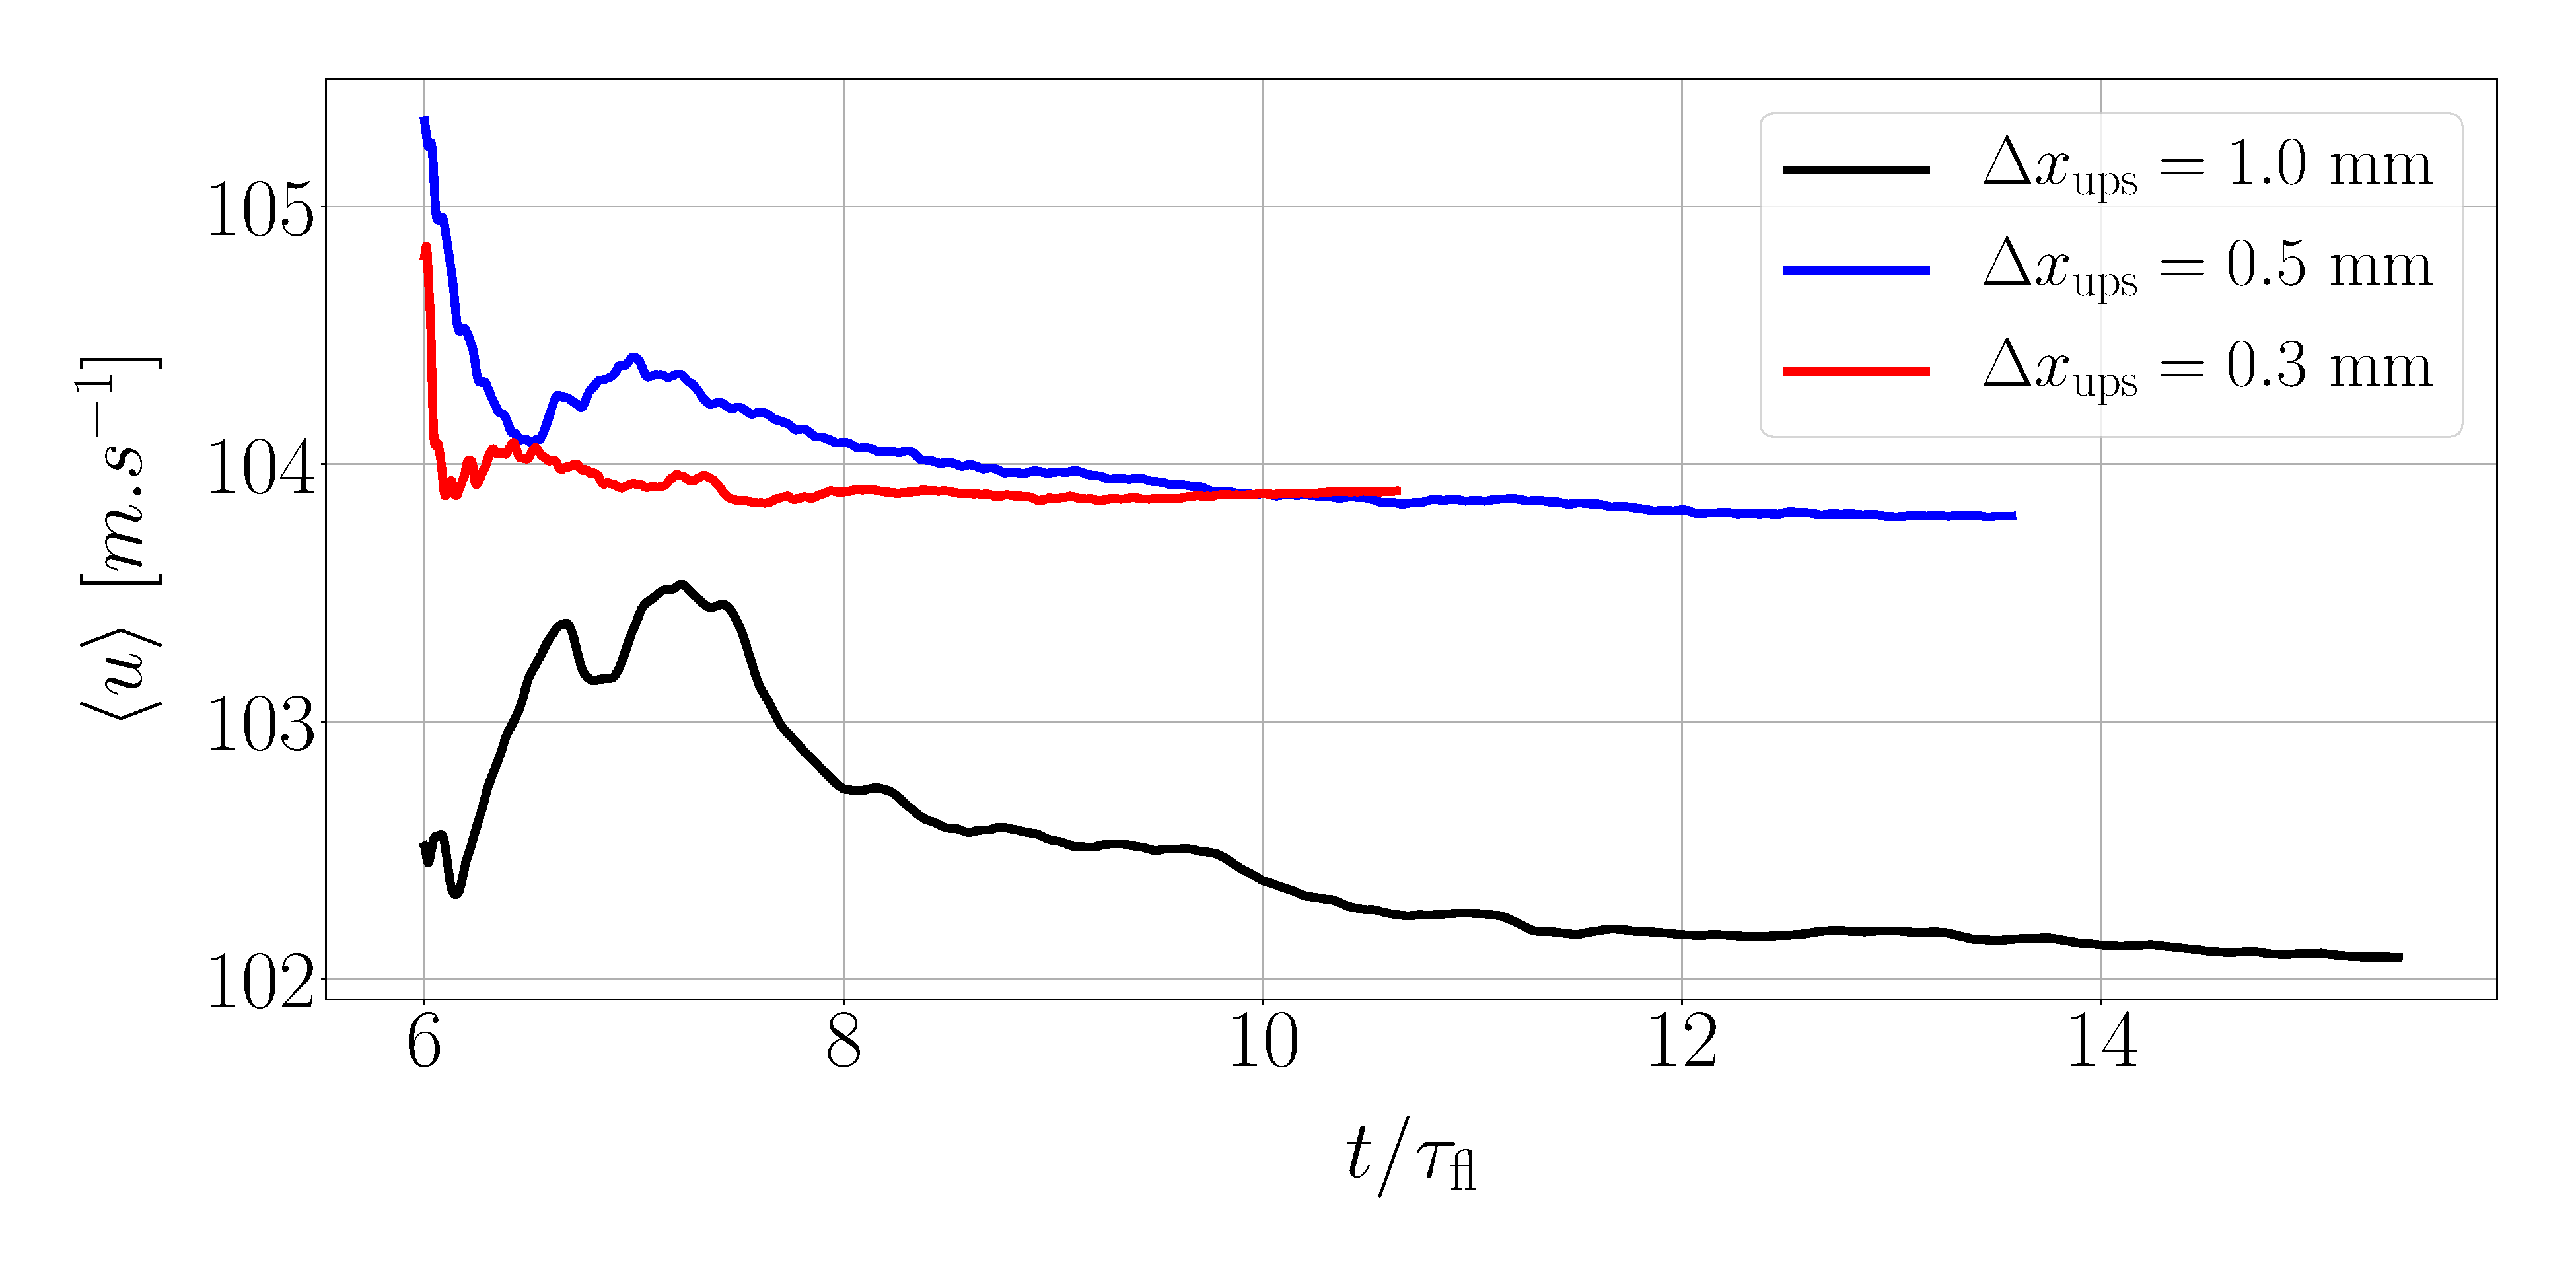
\includegraphics[scale=0.125]{./part2_developments/figures_ch5_resolved_JICF/results_ics_mesh_convergence_line_averages/U_MEAN.pdf}
   \caption{Mean axial velocity}
   %\label{} 
\end{subfigure}
\hfill
\begin{subfigure}[b]{0.45\textwidth}
	\centering
   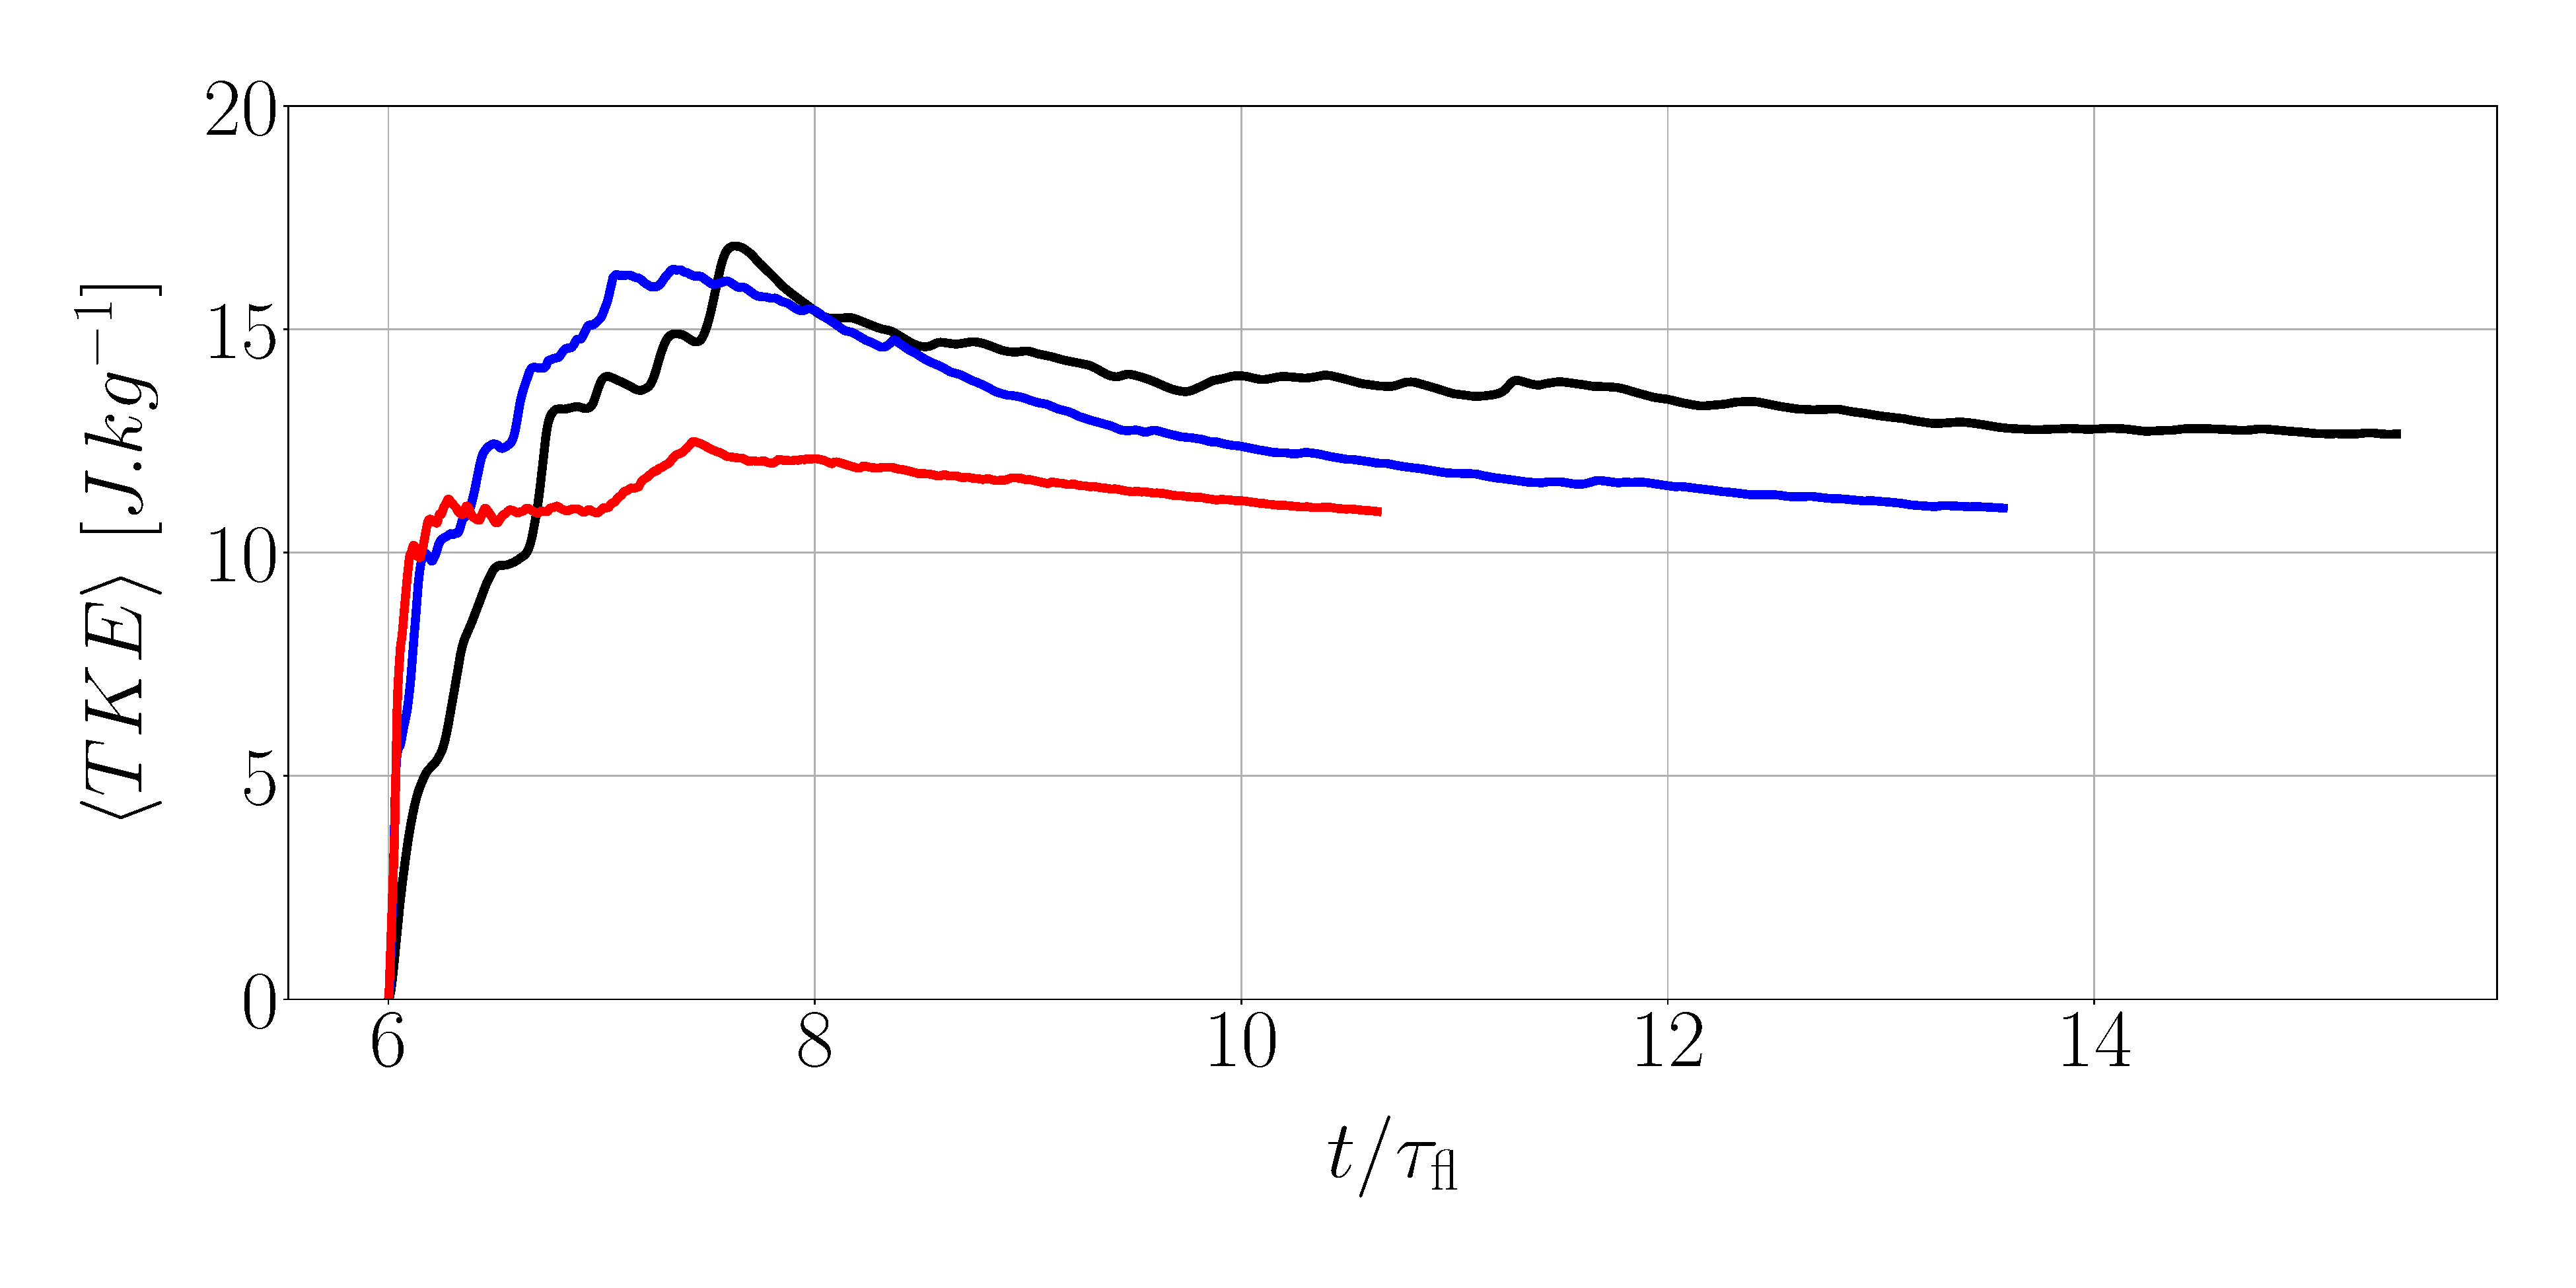
\includegraphics[scale=0.125]{./part2_developments/figures_ch5_resolved_JICF/results_ics_mesh_convergence_line_averages/TKE.pdf}
   \caption{Turbulent Kinetic Energy}
   %\label{}
\end{subfigure}
\caption{Convergence of line-integrated mean axial velocity and TKE with mesh resolution}
\label{fig:mesh_convergence_line_averages}
\end{figure}



Instantaneous snapshots of the fluctuating axial component $u'$ in the middle plane are shown in Figure \ref{fig:ics_mesh_independency_study_up_fields}. The black contours denote the lines with $u' = 0$. As shown, adding turbulence at the inlet introduces fluctuations that are transported downstream the domain. When no turbulence is added, fluctuations are not present (the black contours at the inlet are due to small numerical fluctuations of $u'$) except close to the walls, since they are created inside the boundary layer where flow is turbulent. It is also observed that the characteristic length of the eddies changes when refining the mesh: for the coarsest mesh ($\Delta x_\mathrm{ups} = 1$ mm), these structures are generally large, while refining the mesh to $\Delta x_\mathrm{ups} = 0.5$ and $0.3$ mm reduced their size. 

To assess the quality of the meshes, it is useful to introduce a criterion for measuring the turbulent resolution. For such purpose, the Pope's criterion $M$ is employed \textbf{ref-pope-criterion}, which is calculated from the ratio between the resolved and sub-grid Turbulent Kinetic Energies,  $\mathrm{TKE}$ and $k_\mathrm{sgs}$ respectively:

\begin{equation}
M \left( \textbf{x}, t \right) = \frac{k_\mathrm{sgs} \left( \textbf{x}, t \right)}{k_\mathrm{sgs}  \left( \textbf{x}, t \right) + TKE \left( \textbf{x}, t \right)}
\end{equation}

$M$ represents therefore the ratio between the sub-grid (unresolved) and total TKEs in the domain, and depends on time and space. From its definition it follows that $M = 0$ corresponds to full resolution (i.e. DNS) and $M = 1$ to full modelling (i.e. RANS) of the turbulent flow field. The sub-grid TKE can be obtained from the following expression:


\begin{equation}
k_\mathrm{sgs} = \left( \frac{\nu_t}{0.18 \Delta x} \right)^2
\end{equation}

where $\nu_t$ is the turbulent kinematic viscosity as given by the dynamic Smagorinsky model \citepColor[germano_dynamic_1991]. 

Figure \ref{fig:ics_mesh_independency_study_POPE_M_fields} shows instantenous fields of Pope's criterion for the four simulations performed. As observed, by reducing the element size more regions with values of $M$ closer to $0$ are present. For $\Delta x = 1$ mm there several zones where $M$ has high values. These ones are overall reduced when reducing the cell size to $0.5$ mm and further to $0.3$ mm. Between these last two cell sizes there are also differences in the $M$ field specially far from the walls. For all cases, the $M$ values close to the walls are higher than in the far-field, indicating that a finer resolution would be needed in the walls to properly capture the turbulent features of the boundary layer. Nevertheless, these ones remain around $M \approx 0.5$ for the meshes with $\Delta x = 0.5$ and $0.3$ mm, indicating enough resolution for LES simulations. Regarding the case without turbulence injection for $\Delta x = 0.5$ mm, the $M$ field shows higher values with respect to the case where turbulence is added, specially closer to the inlet and in the regions outside the boundary layer. 

In order to compare quantitatively the difference between meshes, the signals of $u'$ have been monitored with time at the probes shown by the white crosses in the top of Figure \ref{fig:ics_mesh_independency_study_up_fields}. Two probes have been located: one at 1 mm downstream the gaseous inlet (x = 1 mm) and another one 1 mm upstream the liquid injection nozzle (x = 119 mm), both at a height of 8 mm from the bottom walls. The capability of the meshes to transport the resolved turbulent scales, which is of the order of the turbulent fluctuations displayed in Table \ref{tab:jicf_operating_conditions_turbulent_injection_parameters}, is then verified by comparing the fluctuations and spectra obtained with Fast Fourier Transform (FFT) at both probes in Figure \ref{fig:ics_mesh_independency_study_probes}. Time has been normalised with the flow-through time $\tau_\mathrm{fl}$, and the signals are shown for one passage of $\tau_\mathrm{fl}$ for easiness of visualization. For the coarsest mesh $\Delta x_\mathrm{ups} = 1$ mm (Figure \ref{fig:ics_mesh_independency_study_probes_dx1p0}), the $u'$ sampled closer to the nozzle show similar magnitudes but different frequencies to the one from upstream. The spectra confirms this observation: the FFT of probe A displays clearly dominant frequencies at 8, 17 and 25 $\mathrm{kHz}$ with decreasing intensity, while probe A shows also peaks at these locations but also a high predominance of small frequencies. This shows that the mesh with $\Delta x_\mathrm{ups} = 1$ mm is not fully capable of properly transporting the frequencies of the fluctuations. When the mesh is refined to $\Delta x_\mathrm{ups} = 0.5$ mm (Figure \ref{fig:ics_mesh_independency_study_probes_dx0p5}), the small dominant frequencies are no longer relevant and the dominant frequencies are properly captured, as the match in the peaks of the spectra indicate. In this case, the frequencies 8 and 25 $\mathrm{kHz}$ have larger intensity than 17 $\mathrm{kHz}$ . Refining the mesh to $\Delta x_\mathrm{ups} = 0.3$ mm (Figure \ref{fig:ics_mesh_independency_study_probes_dx0p3}) has no longer effect neither in the magnitude of the fluctuations nor in the spectrum. Finally, the fluctuations and FFT of the simulation performed without turbulence injection for the resolution $\Delta x_\mathrm{ups} = 0.5$ mm is shown Figure \ref{fig:ics_mesh_independency_study_probes_dx0p5_no_turb}. As expected, the frequency of the fluctuations  for probe A is minimal (not observed in the $u'$ graph) and predominant frequencies are low. Further downstream some turbulence develops along the channel and created small fluctuations where no clear dominant frequencies are excited. 

\clearpage

\begin{figure}[ht]
\centering
\includeinkscape[inkscapelatex=false,scale=0.75]{./part2_developments/figures_ch5_resolved_JICF/results_ics_mesh_convergence_mesh_and_up/up_field_instantaneous_both}
\caption[Instantaneous $u'$ fields from gaseous simulation for the high Weber case]{Instantaneous $u'$ fields from gaseous simulation for the high Weber case. The right column shows a zoomed-in view of the dashed rectangle from the left column. The black contours indicate the lines with zero instantaneous fluctuation $u' = 0$. From top to bottom $\Delta x_\mathrm{ups} = 1, 0.5, 0.3$ mm.}
\label{fig:ics_mesh_independency_study_up_fields}
\end{figure}

\begin{figure}[ht]
\centering
\includeinkscape[inkscapelatex=false,scale=0.75]{./part2_developments/figures_ch5_resolved_JICF/results_ics_mesh_convergence_POPE/pope_instantaneous_all}
\caption[]{Views of Pope criterion}
\label{fig:ics_mesh_independency_study_POPE_M_fields}
\end{figure}



\begin{figure}[ht]
\centering
\begin{subfigure}[b]{1.0\textwidth}
	\centering   
	\includegraphics[scale=0.28]{./part2_developments/figures_ch5_resolved_JICF/results_ics_mesh_convergence_probes/up_dx1p0.eps}
	\includegraphics[scale=0.28]{./part2_developments/figures_ch5_resolved_JICF/results_ics_mesh_convergence_probes/spectra_linear_scale_dx1p0.eps}
%	\subfloat[\centering]{{\includegraphics[scale=0.20]{./part2_developments/figures_ch5_resolved_JICF/results_ics_mesh_convergence_probes/up_dx1p0.eps} }}%
%    \qquad
%    \subfloat[\centering]{{ \includegraphics[scale=0.20]{./part2_developments/figures_ch5_resolved_JICF/results_ics_mesh_convergence_probes/spectra_linear_scale_dx1p0.eps} }}%
   \caption{Mesh $\Delta x_\mathrm{ups} = 1$ mm}
   \label{fig:ics_mesh_independency_study_probes_dx1p0}
\end{subfigure}


\vskip\baselineskip

\begin{subfigure}[b]{1.0\textwidth}
	\centering
   \includegraphics[scale=0.28]{./part2_developments/figures_ch5_resolved_JICF/results_ics_mesh_convergence_probes/up_dx0p5.eps}
   \includegraphics[scale=0.28]{./part2_developments/figures_ch5_resolved_JICF/results_ics_mesh_convergence_probes/spectra_linear_scale_dx0p5.eps}
   \caption{Mesh $\Delta x_\mathrm{ups} = 0.5$ mm}
   \label{fig:ics_mesh_independency_study_probes_dx0p5}
\end{subfigure}

\vskip\baselineskip

\begin{subfigure}[b]{1.0\textwidth}
	\centering
   \includegraphics[scale=0.28]{./part2_developments/figures_ch5_resolved_JICF/results_ics_mesh_convergence_probes/up_dx0p3.eps}
   \includegraphics[scale=0.28]{./part2_developments/figures_ch5_resolved_JICF/results_ics_mesh_convergence_probes/spectra_linear_scale_dx0p3.eps}
   \caption{{Mesh $\Delta x_\mathrm{ups} = 0.3$ mm}}
   \label{fig:ics_mesh_independency_study_probes_dx0p3}
\end{subfigure}


\vskip\baselineskip

\begin{subfigure}[b]{1.0\textwidth}
	\centering
   \includegraphics[scale=0.28]{./part2_developments/figures_ch5_resolved_JICF/results_ics_mesh_convergence_probes/up_dx0p5_no_turb.eps}
   \includegraphics[scale=0.28]{./part2_developments/figures_ch5_resolved_JICF/results_ics_mesh_convergence_probes/spectra_linear_scale_dx0p5_no_turb.eps}
   \caption{Mesh $\Delta x_\mathrm{ups} = 0.5$ mm without turbulence injection}
   \label{fig:ics_mesh_independency_study_probes_dx0p5_no_turb}
\end{subfigure}

\caption[Frequential analysis of the fluctuations at the sampling probes for the simulations at high Weber number.]{Frequential analysis of the fluctuations at the sampling probes for the simulations at high Weber number. \textsl{Left}: $u'$ fluctuations. \textsl{Right}: spectra of the fluctuations obtained through FFT.}
\label{fig:ics_mesh_independency_study_probes}
\end{figure}




Finally, the profiles of mean axial velocity $\overline{u}$ and TKE are plotting along the vertical line shown in Figure \ref{fig:ics_mesh_independency_study_up_fields} right for the half-width of the channel. The results are shown in Figure \ref{fig:ics_mesh_independency_study_mean_profiles}. 












\clearpage


%\begin{figure}[ht]
%\centering
%\begin{subfigure}[b]{0.3\textwidth}
%	\centering
%   \includegraphics[scale=0.20]{./part2_developments/figures_ch5_resolved_JICF/results_ics_mesh_convergence_probes/up_dx1p0.eps}
%   %\caption{}
%   %\label{} 
%\end{subfigure}
%\hfill
%\begin{subfigure}[b]{0.3\textwidth}
%	\centering
%   \includegraphics[scale=0.20]{./part2_developments/figures_ch5_resolved_JICF/results_ics_mesh_convergence_probes/up_dx0p5.eps}
%   %\caption{}
%   %\label{} 
%\end{subfigure}
%\hfill
%\begin{subfigure}[b]{0.3\textwidth}
%	\centering
%   \includegraphics[scale=0.20]{./part2_developments/figures_ch5_resolved_JICF/results_ics_mesh_convergence_probes/up_dx0p3.eps}
%   %\caption{}
%   %\label{} 
%\end{subfigure}
%
%\vskip\baselineskip
%
%\begin{subfigure}[b]{0.3\textwidth}
%	\centering
%   \includegraphics[scale=0.20]{./part2_developments/figures_ch5_resolved_JICF/results_ics_mesh_convergence_probes/spectra_linear_scale_dx1p0.eps}
%   \caption{}
%   %\label{}
%\end{subfigure}
%\hfill
%\begin{subfigure}[b]{0.3\textwidth}
%	\centering
%   \includegraphics[scale=0.20]{./part2_developments/figures_ch5_resolved_JICF/results_ics_mesh_convergence_probes/spectra_linear_scale_dx0p5.eps}
%   \caption{}
%   %\label{}
%\end{subfigure}
%\hfill
%\begin{subfigure}[b]{0.3\textwidth}
%	\centering
%   \includegraphics[scale=0.20]{./part2_developments/figures_ch5_resolved_JICF/results_ics_mesh_convergence_probes/spectra_linear_scale_dx0p3.eps}
%   \caption{}
%   %\label{}
%\end{subfigure}
%
%\caption[YAP]{Probes}
%\label{fig:ics_mesh_independency_study_probes}
%\end{figure}

\clearpage




%\subsection{Effect of injecting turbulence}

%Once the fine mesh has been chosen as the baseline mesh for the , the effect of injecting turbulence is stated. For this, one simulation without turbulence injection is performed for the high Weber case and compared to the simulation with turbulence injection.


\begin{figure}[ht]
\centering
\begin{subfigure}[b]{0.45\textwidth}
	\centering
   \includegraphics[scale=0.25]{./part2_developments/figures_ch5_resolved_JICF/results_ics_mesh_convergence_mean_profiles/U_MEAN_profiles.pdf}
   \caption{Mean axial velocity}
   %\label{} 
\end{subfigure}
\hfill
\begin{subfigure}[b]{0.45\textwidth}
	\centering
   \includegraphics[scale=0.25]{./part2_developments/figures_ch5_resolved_JICF/results_ics_mesh_convergence_mean_profiles/TKE_profiles.pdf}
   \caption{Turbulent Kinetic Energy}
   %\label{}
\end{subfigure}
\caption{Profiles of $\overline{u}$ and $TKE$ along the line right upstream the injector.}
\label{fig:ics_mesh_independency_study_mean_profiles} 
\end{figure}


\subsection{Initial conditions for low Weber operating point}

From the previous analysis, the ...



\begin{figure}[ht]
	\centering
   \includegraphics[scale=0.28]{./part2_developments/figures_ch5_resolved_JICF/results_ics_mesh_convergence_probes/up_OP2.eps}
   \includegraphics[scale=0.28]{./part2_developments/figures_ch5_resolved_JICF/results_ics_mesh_convergence_probes/spectra_linear_scale_OP2.eps}
   \caption{Mesh $\Delta x_\mathrm{ups} = 0.5$ mm, low-We operating point}
   \label{fig:ics_probes_OP2}
\end{figure}




\section{Definition of characteristic times}

In order to analyse the convergence and results of the four simulations performed, it is useful to relate the simulation times to characteristic times relating the liquid. Three characteristic times are considered in this work:

\begin{itemize}
	
	\item $\tau_\mathrm{liq}$: the characteristic liquid phase time from \citeColor[ranger_aerodynamics_1968], defined as:
	
	\begin{equation}
	\tau_\mathrm{liq} = \sqrt{\frac{\rho_l}{\rho_g}} \frac{d_\mathrm{inj}}{u_g}
	\end{equation}
	
	\item $\tau_\mathrm{ph}$: a characteristic physical time of the JICF, defined as )\textbf{ref:herrmann-2011}):
	
	\begin{equation}
	\label{eq:jicf_tau_injector}
	\tau_\mathrm{ph} = \frac{d_\mathrm{inj}}{u_l}
	\end{equation}

	\item $\tau_\mathrm{str}$: the characteristic time from ligaments stripping from the dense core. This value is obtained by counting the number of liquid structures that emanate from the liquid column in a given time period.

\end{itemize}

For each simulation, the different characteristic times are defined in Table \ref{tab:jicf_characteristic times}. The values $\tau_\mathrm{liq}$ and $\tau_\mathrm{ph}$, depend obviously on the operating condition and not on the mesh resolution, since they are have been obtained from mathematical formulas. On the other hand, the characteristic time $\tau_\mathrm{str}$ has been obtained from each simulation and a dependency on the mesh resolution employed can be expected. 

\begin{table}[!h]
\centering
\caption{Characteristic times in JICF simulations}
\begin{tabular}{lccc}
\thickhline
\textbf{Case} & $\tau_\mathrm{liq}$ [ms] & $\tau_\mathrm{ph}$ [ms] & $\tau_\mathrm{str}$ [ms] \\
\thickhline 
UG75\_DX10  & 0.047 & 0.019 & \\
UG75\_DX20  & 0.047 & 0.019 & \\
UG100\_DX10 & 0.063 & 0.026 & \\
UG100\_DX20 & 0.063 & 0.026 & \\
\thickhline
\end{tabular}
\label{tab:jicf_characteristic times}
\end{table}

We can also define characteristic times as droplets reach the sampling planes. For it, we can make a specific table for each case and each plane:

\begin{table}[!h]
\centering
\caption{Characteristic droplet times in JICF simulations}
\begin{tabular}{lcccc}
\thickhline
\textbf{Case} & $x = 5 mm$ & $x = 10 mm$ & $x = 15 mm$  \\
\thickhline 
UG75\_DX10  & 0.1927 & 0.2952 & -  \\
UG75\_DX20  & 0.2347 & 0.3558 & 0.4567 \\
UG100\_DX10 & 0.1437 & 0.2187 & - \\
UG100\_DX20 & 0.1768 & 0.2584 & 0.3628 \\
\thickhline
\end{tabular}
\label{tab:jicf_characteristic_droplet_sampling_times}
\end{table}


%\section{Results}
%\label{sec:results_JICF_resolved}

\section{Jet topology}


\subsection{Flow establishment}

A non-dimensional time can be defined as

\begin{equation}
t^* = \frac{t}{\tau_\mathrm{ph}}
\end{equation}

The increase in mesh elements is seen in Figure \ref{fig:JICF_nelem_increase}.

\begin{figure}[ht]
\centering
	\centering
   \includegraphics[scale=0.25]{./part2_developments/figures_ch5_resolved_JICF/JICF_nelem_increase}
   %\label{} 
\caption{Evolution of number of mesh elements with time in JICF simulations}
\label{fig:JICF_nelem_increase}
\end{figure}

\clearpage

\begin{figure}[ht]
\centering
\includeinkscape[inkscapelatex=false,scale=0.8]{./part2_developments/figures_ch5_resolved_JICF/JICF_establishment_UG100_lateral}
\caption[Lateral view of high We jet at several time instants. ]{Lateral view of high We jet at several time instants. \textsl{Left}: UG100\_DX20. \textsl{Right}: UG100\_DX10.}
\label{fig:JICF_establishment_UG100_lateral}
\end{figure}

\clearpage

\begin{figure}[ht]
\centering
\includeinkscape[inkscapelatex=false,scale=0.8]{./part2_developments/figures_ch5_resolved_JICF/JICF_establishment_UG100_front}
\caption[Front view of high We jet at several time instants. ]{Front view of high We jet at several time instants. \textsl{Left}: UG100\_DX20. \textsl{Right}: UG100\_DX10.}
\label{fig:JICF_establishment_UG100_front}
\end{figure}
\clearpage

\clearpage

\begin{figure}[ht]
\centering
\includeinkscape[inkscapelatex=false,scale=0.8]{./part2_developments/figures_ch5_resolved_JICF/JICF_establishment_UG100_top}
\caption[Top view of high We jet at several time instants. ]{Top view of high We jet at several time instants. \textsl{Left}: UG100\_DX20. \textsl{Right}: UG100\_DX10.}
\label{fig:JICF_establishment_UG100_top}
\end{figure}




\clearpage

\begin{figure}[ht]
\centering
\includeinkscape[inkscapelatex=false,scale=0.8]{./part2_developments/figures_ch5_resolved_JICF/JICF_establishment_UG75_lateral}
\caption[Lateral view of low We jet at several time instants. ]{Lateral view of low We jet at several time instants. \textsl{Left}: UG75\_DX20. \textsl{Right}: UG75\_DX10.}
\label{fig:JICF_establishment_UG75_lateral}
\end{figure}

\clearpage

\begin{figure}[ht]
\centering
\includeinkscape[inkscapelatex=false,scale=0.8]{./part2_developments/figures_ch5_resolved_JICF/JICF_establishment_UG75_front}
\caption[Front view of low We jet at several time instants. ]{Front view of low We jet at several time instants. \textsl{Left}: UG75\_DX20. \textsl{Right}: UG75\_DX10.}
\label{fig:JICF_establishment_UG75_front}
\end{figure}

\clearpage

\begin{figure}[ht]
\centering
\includeinkscape[inkscapelatex=false,scale=0.8]{./part2_developments/figures_ch5_resolved_JICF/JICF_establishment_UG75_top}
\caption[Top view of low We jet at several time instants. ]{Top view of low We jet at several time instants. \textsl{Left}: UG75\_DX20. \textsl{Right}: UG75\_DX10.}
\label{fig:JICF_establishment_UG75_top}
\end{figure}

\clearpage

\subsection{Jet breakup}


\section{Jet trajectories}
\label{subsec:ch5_jet_trajectories_results}

Different methods to obtain trajectories from resolved simulations were proposed in $\S$\ref{sec:ch5_tools_jicf_trajectories}. These methods are summarized in Table \ref{tab:jicf_tools_trajectories_obtention}. In this section, firstly  the four methods described are applied to the simulation UG100\_DX20, the trajectories obtained are then compared and discussed. Secondly, the method MEAN\_GRAD is chosen to perform experimental validation with all simulations from Table \ref{tab:jicf_resolved_simulations_performed}, since this is the numerical methodology more similar to the way in which the experimental correlations in \citeColor[becker_breakup_2002] are obtained.

The accuracy of the mean numerical trajectories can be quantitatively assessed by defining a $L_2$ error as in Eq.~(\ref{eq:L2_JICF}): 

\begin{equation}
\label{eq:L2_JICF}
    L_2 = \sqrt{\frac{1}{N}   \sum_{i=1}^N \left( \frac{z}{d_\mathrm{inj}} \Bigr|_{\mathrm{num},i} -   \frac{z}{d_\mathrm{inj}} \Bigr|_{\mathrm{exp},i} \right)^2}
\end{equation}



We can also define an error along the trajectory as follows:



\begin{equation}
\varepsilon_i  =  \frac{ \frac{z}{d_\mathrm{inj}} \Bigr|_{\mathrm{num},i} - \frac{z}{d_\mathrm{inj}} \Bigr|_{\mathrm{exp},i} }{ \frac{z}{d_\mathrm{inj}} \Bigr|_{\mathrm{exp},i} }
\end{equation}

\begin{equation}
\varepsilon_i  =  \frac{ z/d_\mathrm{inj} \Bigr|_{\mathrm{num},i} - z/d_\mathrm{inj} \Bigr|_{\mathrm{exp},i} }{ z/d_\mathrm{inj} \Bigr|_{\mathrm{exp},i} }
\end{equation}


\subsection{Comparison of methods}


\begin{figure}[ht]
\centering
\begin{subfigure}[b]{0.45\textwidth}
	\centering
   \includegraphics[scale=0.15]{./part2_developments/figures_ch5_resolved_JICF/results_trajectories/methods_comparison_trajectories_q6uG100.pdf}
   \caption{Mean trajectories}
   %\label{} 
\end{subfigure}
\hfill
\begin{subfigure}[b]{0.45\textwidth}
	\centering
   \includegraphics[scale=0.15]{./part2_developments/figures_ch5_resolved_JICF/results_trajectories/methods_comparison_L2_evolution_q6uG100.pdf}
   \caption{$L_2$ error evolution}
   %\label{}
\end{subfigure}
\caption{Trajectories and $L_2$ errors obtained with different methods for case UG100\_DX20}
\label{fig:JICF_trajectories_and_L2_comparison}
\end{figure}

\subsection{Experimental validation}

\begin{figure}[ht]
\centering
\begin{subfigure}[b]{0.45\textwidth}
	\centering
   \includegraphics[scale=0.15]{./part2_developments/figures_ch5_resolved_JICF/results_trajectories/methods_expe_validation_trajectories_q6uG75.pdf}
   \caption{Low $We$}
   %\label{} 
\end{subfigure}
\hfill
\begin{subfigure}[b]{0.45\textwidth}
	\centering
   \includegraphics[scale=0.15]{./part2_developments/figures_ch5_resolved_JICF/results_trajectories/methods_expe_validation_trajectories_q6uG100.pdf}
   \caption{Low $We$}
   %\label{}
\end{subfigure}
\caption{Trajectories obtained with methods MEAN\_GRAD}
\label{fig:JICF_trajectories_validation}
\end{figure}


\section{Direct measurement of liquid flow rates}

Liquid fluxes have been measured in the resolved simulations at the planes shown in Figure \ref{fig:jicf_interior_boundaries_surface_measurements}. In the coarse simulations done with a mesh resolution of $\Delta x_\mathrm{min} = 20 \mu m$, fluxes have been obtained in all planes shown in the sketch. For the fine simulations, results were collected up to x = 10 mm since the liquid was removed shortly afterwards.

\subsection{Obtention of total flow rate}

The time evolution of flow rates for case UG100\_DX20 is shown in Figure \ref{fig:IB_liquid_flow_rate_inst_evolution_UG100_DX20} for both crossflow and filming planes. For the crossflow planes, the 

%\begin{figure}[h!]
%\centering
%\includegraphics[scale=0.6]{./part2_developments/figures_ch5_resolved_JICF/flow_rates_ibs/uG100_dx20_QL_isox_time_evol.eps}
%\caption{Liquid flow rate evolution with time in the}
%\label{fig:graphite_cp}
%\end{figure}

\begin{figure}[ht]
\centering
\begin{subfigure}[b]{0.45\textwidth}
	\centering
   \includegraphics[scale=0.15]{./part2_developments/figures_ch5_resolved_JICF/flow_rates_ibs/uG100_dx20_QL_isox_time_evol.eps}
   %\caption{}
   %\label{} 
\end{subfigure}
\begin{subfigure}[b]{0.45\textwidth}
	\centering
   \includegraphics[scale=0.15]{./part2_developments/figures_ch5_resolved_JICF/flow_rates_ibs/uG100_dx20_QL_filming_time_evol.eps}
   %\caption{}
   %\label{}
\end{subfigure}
\caption{Time evolution of instantaneous liquid flow rates for case UG100\_DX20. \textbf{Left}: planes normal to crossflow. \textbf{Right}: filming planes.}
\label{fig:IB_liquid_flow_rate_inst_evolution_UG100_DX20}
\end{figure}

\newpage

\begin{figure}[ht]
\centering
\begin{subfigure}[b]{0.45\textwidth}
	\centering
   \includegraphics[scale=0.17]{./part2_developments/figures_ch5_resolved_JICF/flow_rates_ibs/uG100_dx20_QL_isox_mean_time_convergence.eps}
   \caption{Mean $Q_l$ in crossflow planes}
   %\label{} 
\end{subfigure}
\hfill
\begin{subfigure}[b]{0.45\textwidth}
	\centering
   \includegraphics[scale=0.17]{./part2_developments/figures_ch5_resolved_JICF/flow_rates_ibs/uG100_dx20_QL_isox_RMS_time_convergence.eps}
   \caption{RMS $Q_l$ in crossflow planes}
   %\label{}
\end{subfigure}
\vskip\baselineskip
\begin{subfigure}[b]{0.45\textwidth}
	\centering
   \includegraphics[scale=0.17]{./part2_developments/figures_ch5_resolved_JICF/flow_rates_ibs/uG100_dx20_QL_filming_mean_time_convergence.eps}
   \caption{Mean $Q_l$ in filming planes}
   %\label{} 
\end{subfigure}
\hfill
\begin{subfigure}[b]{0.45\textwidth}
	\centering
   \includegraphics[scale=0.17]{./part2_developments/figures_ch5_resolved_JICF/flow_rates_ibs/uG100_dx20_QL_filming_RMS_time_convergence.eps}
   \caption{RMS $Q_l$ in filming planes}
   %\label{}
\end{subfigure}
\caption{Time evolution of mean and RMS liquid flow rates for case UG100\_DX20.}
\label{fig:IB_liquid_flow_rate_mean_RMS_evolution_UG100_DX20}
\end{figure}

\newpage

\begin{figure}[ht]
\centering
\begin{subfigure}[b]{0.45\textwidth}
	\centering
   \includegraphics[scale=0.10]{./part2_developments/figures_ch5_resolved_JICF/flow_rates_ibs/uG100_dx20_QL_isox_bar_plot.eps}
   \caption{Case UG100\_DX20: crossflow planes}
   %\label{} 
\end{subfigure}
\hfill
\begin{subfigure}[b]{0.45\textwidth}
	\centering
   \includegraphics[scale=0.10]{./part2_developments/figures_ch5_resolved_JICF/flow_rates_ibs/uG100_dx20_QL_filming_bar_plot.eps}
   \caption{Case UG100\_DX20: filming planes}
   %\label{}
\end{subfigure}
\vskip\baselineskip
\begin{subfigure}[b]{0.45\textwidth}
	\centering
   \includegraphics[scale=0.10]{./part2_developments/figures_ch5_resolved_JICF/flow_rates_ibs/uG100_dx10_QL_isox_bar_plot.eps}
   \caption{Case UG100\_DX10: crossflow planes}
   %\label{} 
\end{subfigure}
\hfill
\begin{subfigure}[b]{0.45\textwidth}
	\centering
   \includegraphics[scale=0.10]{./part2_developments/figures_ch5_resolved_JICF/flow_rates_ibs/uG100_dx10_QL_filming_bar_plot.eps}
   \caption{Case UG100\_DX10: filming planes}
   %\label{}
\end{subfigure}

\vskip\baselineskip

\begin{subfigure}[b]{0.45\textwidth}
	\centering
   \includegraphics[scale=0.10]{./part2_developments/figures_ch5_resolved_JICF/flow_rates_ibs/uG75_dx20_QL_isox_bar_plot.eps}
   \caption{Case UG75\_DX20: crossflow planes}
   %\label{} 
\end{subfigure}
\hfill
\begin{subfigure}[b]{0.45\textwidth}
	\centering
   \includegraphics[scale=0.10]{./part2_developments/figures_ch5_resolved_JICF/flow_rates_ibs/uG75_dx20_QL_filming_bar_plot.eps}
   \caption{Case UG75\_DX20: filming planes}
   %\label{}
\end{subfigure}
\vskip\baselineskip
\begin{subfigure}[b]{0.45\textwidth}
	\centering
   \includegraphics[scale=0.10]{./part2_developments/figures_ch5_resolved_JICF/flow_rates_ibs/uG75_dx10_QL_isox_bar_plot.eps}
   \caption{Case UG75\_DX10: crossflow planes}
   %\label{} 
\end{subfigure}
\hfill
\begin{subfigure}[b]{0.45\textwidth}
	\centering
   \includegraphics[scale=0.10]{./part2_developments/figures_ch5_resolved_JICF/flow_rates_ibs/uG75_dx10_QL_filming_bar_plot.eps}
   \caption{Case UG75\_DX10: filming planes}
   %\label{}
\end{subfigure}
\caption[Mean flow rates (bars) and RMS (lines) obtained with interior boundaries for each simulation performed]{Mean flow rates (bars) and RMS (lines) obtained with interior boundaries for each simulation performed. }
\label{fig:JICF_ibs_flow_rates_bars_plots}
\end{figure}









\subsection{Spatial distribution of flow rates in crossflow planes}




\newpage

\subsection{Mass conservation in ACLS}

%\subsubsection{Sampling procedure for droplets}

\newpage

\section{Spray characterization}

The number of droplets accumulated in each sampling plane for all the simulations performed in shown in Figure \ref{tab:jicf_Ndr_accumulated}.

\begin{table}[!h]
\centering
\caption{Number of droplets accumulated in JICF simulations}
\begin{tabular}{rcccc}
\thickhline
\textbf{Case} & $x = 5$ mm & $x = 10$ mm & $x = 15$ mm  & $x = 20$ mm \\
\thickhline 
UG75\_DX10  & 14233 & 20677 & - & - \\
UG75\_DX20  &  6882 & 12224 & 12077 & 9440 \\
UG100\_DX10 & 16442 & 11087 & - & -\\
UG100\_DX20 & 21824 & 17793 & 9476 & 11041 \\
\thickhline
\end{tabular}
\label{tab:jicf_Ndr_accumulated}
\end{table}

For the histograms, we can see 2013 Vie.


\subsection{Deformation variation with axial distance}

\subsection{Granulometry}

Sprays generated by atomization processes can be characterized by means of distributions. A given spray where the sizes of the droplets are known can be studied by representing distributions which express the probability of finding a droplet diameter or volume in that spray. Size distributions are usually representing by the notation $f_0 \left( D \right)$, while volume distributions are denoted by $f_3 \left( D \right)$. Two types of distributions are possible: discrete (histograms) or continuous. In the former, the spectrum of droplets size is divided into several range of droplets named bins or classes, and the number of droplets comprised within each class each counted. Histograms are the usual way of representing the granulometry when the size of droplets is directly available, such as in most experimental campaings and computational studies resolving atomization. Continuous distributions, however, are often used to fit discrete distributions obtained experimentally and are used for making simplified models for spray injection in lagrangian simulations, since they can represent the spray by functions depending on few parameters. Examples of function widely used in sprays are the lognormal, Rosin-Rammler and Nukiyama-Tanasama distributions \citepColor[lefebvre_atomization_2017]. 

Since in the resolved simulations performed in the work the size and volume of droplets are known (formally, the volume is known but the size is estimated with Eq. \ref{eq:ch4_r_equivalent_calculation}), probability histograms can be plotted. Figure \ref{fig:JICF_histograms_ug100_dx20} shows size (left) and volume (right) histograms for the sprays obtained from the case UG100\_DX20. The number of classes has been calculated according to Rice's rule, which estimates this value as $N_\mathrm{bins} = \sqrt[3]{2 N_\mathrm{dr}}$ \citepColor[terrel_oversmoothed_1985].




Size distributions can be represented by means of histograms relating the probability of finding a droplet with a given size with respect to the diameter, $f_0 \left( D \right)$.



In \citeColor[lefebvre_atomization_2017] ...



\textbf{Log-normal distribution}. This distribution function is more representative of certain types of atomizers, such as the spray produced by the jet in crossflow. In contrast to the normal distribution, the log-normal distribution takes the logarithm of the particle diameter as a variable. It is given by the following expression, where $\overline{D}_{ng}$ is the geometric mean size of the logarithmic droplet size and $s_g$ is the geometric standard deviation:

\begin{equation}
 f_0 \left( D \right) = \frac{d N}{d D} =  \frac{1}{D  \sqrt{2 \pi \ln \left( s_g \right)^2}} \exp \left[ - \frac{1}{2 } \left( \frac{\ln D - \ln \overline{D}_{ng}}{\ln s_g}   \right)^2 \right]
\end{equation}
%
\begin{equation}
\overline{D}_{ng} = \exp \left(  \frac{\sum_i \ln D_i }{N_\mathrm{droplets}} \right) 
\end{equation}

\begin{equation}
s_g = \exp \sqrt{  \frac{\sum_i \ln \left( D_i / \overline{D}_{ng} \right) ^2 }{N_\mathrm{droplets}} }
\end{equation}




\begin{figure}[ht]
\centering
\begin{subfigure}[b]{0.45\textwidth}
	\centering
   \includegraphics[scale=0.30]{./part2_developments/figures_ch5_resolved_JICF/spray_distributions/uG100_dx20_x05_number_histogram.eps}
   \caption{x = 5 mm, number histogram}
   %\label{} 
\end{subfigure}
\hfill
\begin{subfigure}[b]{0.45\textwidth}
	\centering
   \includegraphics[scale=0.30]{./part2_developments/figures_ch5_resolved_JICF/spray_distributions/uG100_dx20_x05_volume_histogram.eps}
   \caption{x = 5 mm, volume histogram}
   %\label{}
\end{subfigure}
\vskip\baselineskip
\begin{subfigure}[b]{0.45\textwidth}
	\centering
   \includegraphics[scale=0.30]{./part2_developments/figures_ch5_resolved_JICF/spray_distributions/uG100_dx20_x10_number_histogram.eps}
   \caption{x = 10 mm, number histogram}
   %\label{} 
\end{subfigure}
\hfill
\begin{subfigure}[b]{0.45\textwidth}
	\centering
   \includegraphics[scale=0.30]{./part2_developments/figures_ch5_resolved_JICF/spray_distributions/uG100_dx20_x10_volume_histogram.eps}
   \caption{x = 10 mm, volume histogram}
   %\label{}
\end{subfigure}
\vskip\baselineskip
\begin{subfigure}[b]{0.45\textwidth}
	\centering
   \includegraphics[scale=0.30]{./part2_developments/figures_ch5_resolved_JICF/spray_distributions/uG100_dx20_x15_number_histogram.eps}
   \caption{x = 15 mm, number histogram}
   %\label{} 
\end{subfigure}
\hfill
\begin{subfigure}[b]{0.45\textwidth}
	\centering
   \includegraphics[scale=0.30]{./part2_developments/figures_ch5_resolved_JICF/spray_distributions/uG100_dx20_x15_volume_histogram.eps}
   \caption{x = 15 mm, volume histogram}
   %\label{}
\end{subfigure}
\vskip\baselineskip
\begin{subfigure}[b]{0.45\textwidth}
	\centering
   \includegraphics[scale=0.30]{./part2_developments/figures_ch5_resolved_JICF/spray_distributions/uG100_dx20_x20_number_histogram.eps}
   \caption{x = 20 mm, number histogram}
   %\label{} 
\end{subfigure}
\hfill
\begin{subfigure}[b]{0.45\textwidth}
	\centering
   \includegraphics[scale=0.30]{./part2_developments/figures_ch5_resolved_JICF/spray_distributions/uG100_dx20_x20_volume_histogram.eps}
   \caption{x = 20 mm, volume histogram}
   %\label{}
\end{subfigure}
\caption{Histograms and lognormal fits for sampling planes in case UG100\_DX20}
\label{fig:JICF_histograms_ug100_dx20}
\end{figure}


\begin{figure}[ht]
\centering
   \includegraphics[scale=0.30]{./part2_developments/figures_ch5_resolved_JICF/SMD_values.eps}
   \caption{Evolution of SMD with axial distance for each simulation}
   \label{}
\end{figure}

\subsection{Definition of characteristic times}

Several characteristic times can be defined in a jet in crossflow:

\begin{itemize}

	\item Characteristic time of ligaments passage at given planes, $t_\mathrm{pas}$
	
	\item Characteristic time related to the frequency of the instabilities causing column breakup, $t_\mathrm{ins}$
	
	\item Physical definition according to ...

\end{itemize}



\section{Dense core characterization}
\label{subsec:ch5_dense_core_in_ACLS_simus}

Resolved simulations are characterized by the presence of the dense core, whose presence perturbs the incoming air and creates turbulence downstream the injector. To illustrate this disturbance, the instantaneous axial fluctuations $u'$ and the jet interface are plotted in the middle plane y = 0 in Figure \ref{fig:results_dense_core_modeling_up_field} left. As shown, the jet presence

\begin{figure}[ht]
\centering
\includeinkscape[inkscapelatex=false,scale=0.75]{./part2_developments/figures_ch5_resolved_JICF/results_dense_core_modeling/up_field_instantaneous}
\caption[Perturbation effect of the liquid dense core in the gaseous field.]{Instantaneous $u'$ field in a JICF simulation from case UG100\_DX20. The black contours indicate the lines with zero instantaneous fluctuation $u' = 0$, while the white contours denote the location of the interface at the plane.}
\label{fig:results_dense_core_modeling_up_field}
\end{figure}



$\S$\ref{sec:ch4_dense_core_modelling}.

\section{Frequential analysis}

A spectral analysis is performed to obtain the characteristic breakup frequencies. There are several ways to obtain the desired frequencies:

\begin{itemize}

	\item Use Proper Orthogonal Decomposition (POD) technique (2018 Prakash, Mukundan). This is out of the scope of this work.
	
	\item Get evolution of breakup point with time: $x_b \left( t \right)$, $z_b \left( t \right)$, then get the frequency spectrum  (2010 Wang, 2018 Prakash). Not sure we can do this with our available data, so not envisageable now.
	
	\item Locate probes along liquid column, get liquid presence rate with time. This is the one !!

\end{itemize}

\section{Computational performances}
\label{subsec:ch5_computational_performances}

%\subsection{Feeding the models (??)}
%Find a more attractive name

\section{Learning injectors}



\subsection{Spatial discretization of sprays}

\clearpage

\subsection{Case UG75\_DX10}



%%%%%%%%%%%%%%%% UG75_DX10, x = 5 mm


\begin{figure}[h!]
\flushleft
\begin{subfigure}[b]{0.22\textwidth}
	\centering
   \includegraphics[scale=0.17]{./part2_developments/figures_ch5_resolved_JICF/injectors_SLI/uG75_dx10_x05_SMD_map.eps}
   %\caption{Case UG100\_DX20: crossflow planes}
   %\label{} 
\end{subfigure}
   \hspace{0.17in}
\begin{subfigure}[b]{0.22\textwidth}
	\centering
   \includegraphics[scale=0.17]{./part2_developments/figures_ch5_resolved_JICF/injectors_SLI/uG75_dx10_x05_ux_mean_map.eps}
   %\caption{Case UG100\_DX20: filming planes}
   %\label{}
\end{subfigure}
   \hspace{0.17in}
\begin{subfigure}[b]{0.22\textwidth}
	\centering
   \includegraphics[scale=0.17]{./part2_developments/figures_ch5_resolved_JICF/injectors_SLI/uG75_dx10_x05_uy_mean_map.eps}
   %\caption{Case UG100\_DX10: crossflow planes}
   %\label{} 
\end{subfigure}
   \hspace{0.17in}
\begin{subfigure}[b]{0.22\textwidth}
	\centering
   \includegraphics[scale=0.17]{./part2_developments/figures_ch5_resolved_JICF/injectors_SLI/uG75_dx10_x05_uz_mean_map.eps}
   %\caption{Case UG100\_DX10: filming planes}
   %\label{}
\end{subfigure}

\vskip\baselineskip

\begin{subfigure}[b]{0.22\textwidth}
	\centering
   \includegraphics[scale=0.17]{./part2_developments/figures_ch5_resolved_JICF/injectors_SLI/uG75_dx10_x05_volume_flux_map.eps}
   %\caption{Case UG100\_DX20: crossflow planes}
   %\label{} 
\end{subfigure}
   \hspace{0.17in}
\begin{subfigure}[b]{0.22\textwidth}
	\centering
   \includegraphics[scale=0.17]{./part2_developments/figures_ch5_resolved_JICF/injectors_SLI/uG75_dx10_x05_ux_rms_map.eps}
   %\caption{Case UG100\_DX20: filming planes}
   %\label{}
\end{subfigure}
   \hspace{0.17in}
\begin{subfigure}[b]{0.22\textwidth}
	\centering
   \includegraphics[scale=0.17]{./part2_developments/figures_ch5_resolved_JICF/injectors_SLI/uG75_dx10_x05_uy_rms_map.eps}
   %\caption{Case UG100\_DX10: crossflow planes}
   %\label{} 
\end{subfigure}
   \hspace{0.17in}
\begin{subfigure}[b]{0.22\textwidth}
	\centering
   \includegraphics[scale=0.17]{./part2_developments/figures_ch5_resolved_JICF/injectors_SLI/uG75_dx10_x05_uz_rms_map.eps}
   %\caption{Case UG100\_DX10: filming planes}
   %\label{}
\end{subfigure}
\caption{Spray states at x = 5 mm for case UG75\_DX10}
\label{fig:injectors_sli_uG75_dx10_x05}
\end{figure}


%%%%%%%%%%%%%%%% UG75_DX10, x = 10 mm


\begin{figure}[h!]
\flushleft
\begin{subfigure}[b]{0.22\textwidth}
	\centering
   \includegraphics[scale=0.17]{./part2_developments/figures_ch5_resolved_JICF/injectors_SLI/uG75_dx10_x10_SMD_map.eps}
   %\caption{Case UG100\_DX20: crossflow planes}
   %\label{} 
\end{subfigure}
   \hspace{0.17in}
\begin{subfigure}[b]{0.22\textwidth}
	\centering
   \includegraphics[scale=0.17]{./part2_developments/figures_ch5_resolved_JICF/injectors_SLI/uG75_dx10_x10_ux_mean_map.eps}
   %\caption{Case UG100\_DX20: filming planes}
   %\label{}
\end{subfigure}
   \hspace{0.17in}
\begin{subfigure}[b]{0.22\textwidth}
	\centering
   \includegraphics[scale=0.17]{./part2_developments/figures_ch5_resolved_JICF/injectors_SLI/uG75_dx10_x10_uy_mean_map.eps}
   %\caption{Case UG100\_DX10: crossflow planes}
   %\label{} 
\end{subfigure}
   \hspace{0.17in}
\begin{subfigure}[b]{0.22\textwidth}
	\centering
   \includegraphics[scale=0.17]{./part2_developments/figures_ch5_resolved_JICF/injectors_SLI/uG75_dx10_x10_uz_mean_map.eps}
   %\caption{Case UG100\_DX10: filming planes}
   %\label{}
\end{subfigure}

\vskip\baselineskip

\begin{subfigure}[b]{0.22\textwidth}
	\centering
   \includegraphics[scale=0.17]{./part2_developments/figures_ch5_resolved_JICF/injectors_SLI/uG75_dx10_x10_volume_flux_map.eps}
   %\caption{Case UG100\_DX20: crossflow planes}
   %\label{} 
\end{subfigure}
   \hspace{0.17in}
\begin{subfigure}[b]{0.22\textwidth}
	\centering
   \includegraphics[scale=0.17]{./part2_developments/figures_ch5_resolved_JICF/injectors_SLI/uG75_dx10_x10_ux_rms_map.eps}
   %\caption{Case UG100\_DX20: filming planes}
   %\label{}
\end{subfigure}
   \hspace{0.17in}
\begin{subfigure}[b]{0.22\textwidth}
	\centering
   \includegraphics[scale=0.17]{./part2_developments/figures_ch5_resolved_JICF/injectors_SLI/uG75_dx10_x10_uy_rms_map.eps}
   %\caption{Case UG100\_DX10: crossflow planes}
   %\label{} 
\end{subfigure}
   \hspace{0.17in}
\begin{subfigure}[b]{0.22\textwidth}
	\centering
   \includegraphics[scale=0.17]{./part2_developments/figures_ch5_resolved_JICF/injectors_SLI/uG75_dx10_x10_uz_rms_map.eps}
   %\caption{Case UG100\_DX10: filming planes}
   %\label{}
\end{subfigure}
\caption{Spray states at x = 10 mm for case UG75\_DX10}
\label{fig:injectors_sli_uG75_dx10_x10}
\end{figure}


\clearpage

\subsection{Case UG75\_DX20}



%%%%%%%%%%%%%%%% UG75_DX20, x = 5 mm


\begin{figure}[h!]
\flushleft
\begin{subfigure}[b]{0.22\textwidth}
	\centering
   \includegraphics[scale=0.17]{./part2_developments/figures_ch5_resolved_JICF/injectors_SLI/uG75_dx20_x05_SMD_map.eps}
   %\caption{Case UG100\_DX20: crossflow planes}
   %\label{} 
\end{subfigure}
   \hspace{0.17in}
\begin{subfigure}[b]{0.22\textwidth}
	\centering
   \includegraphics[scale=0.17]{./part2_developments/figures_ch5_resolved_JICF/injectors_SLI/uG75_dx20_x05_ux_mean_map.eps}
   %\caption{Case UG100\_DX20: filming planes}
   %\label{}
\end{subfigure}
   \hspace{0.17in}
\begin{subfigure}[b]{0.22\textwidth}
	\centering
   \includegraphics[scale=0.17]{./part2_developments/figures_ch5_resolved_JICF/injectors_SLI/uG75_dx20_x05_uy_mean_map.eps}
   %\caption{Case UG100\_DX10: crossflow planes}
   %\label{} 
\end{subfigure}
   \hspace{0.17in}
\begin{subfigure}[b]{0.22\textwidth}
	\centering
   \includegraphics[scale=0.17]{./part2_developments/figures_ch5_resolved_JICF/injectors_SLI/uG75_dx20_x05_uz_mean_map.eps}
   %\caption{Case UG100\_DX10: filming planes}
   %\label{}
\end{subfigure}

\vskip\baselineskip

\begin{subfigure}[b]{0.22\textwidth}
	\centering
   \includegraphics[scale=0.17]{./part2_developments/figures_ch5_resolved_JICF/injectors_SLI/uG75_dx20_x05_volume_flux_map.eps}
   %\caption{Case UG100\_DX20: crossflow planes}
   %\label{} 
\end{subfigure}
   \hspace{0.17in}
\begin{subfigure}[b]{0.22\textwidth}
	\centering
   \includegraphics[scale=0.17]{./part2_developments/figures_ch5_resolved_JICF/injectors_SLI/uG75_dx20_x05_ux_rms_map.eps}
   %\caption{Case UG100\_DX20: filming planes}
   %\label{}
\end{subfigure}
   \hspace{0.17in}
\begin{subfigure}[b]{0.22\textwidth}
	\centering
   \includegraphics[scale=0.17]{./part2_developments/figures_ch5_resolved_JICF/injectors_SLI/uG75_dx20_x05_uy_rms_map.eps}
   %\caption{Case UG100\_DX10: crossflow planes}
   %\label{} 
\end{subfigure}
   \hspace{0.17in}
\begin{subfigure}[b]{0.22\textwidth}
	\centering
   \includegraphics[scale=0.17]{./part2_developments/figures_ch5_resolved_JICF/injectors_SLI/uG75_dx20_x05_uz_rms_map.eps}
   %\caption{Case UG100\_DX10: filming planes}
   %\label{}
\end{subfigure}
\caption{Spray states at x = 5 mm for case UG75\_DX20}
\label{fig:injectors_sli_uG75_dx20_x05}
\end{figure}


%%%%%%%%%%%%%%%% UG75_DX10, x = 10 mm


\begin{figure}[h!]
\flushleft
\begin{subfigure}[b]{0.22\textwidth}
	\centering
   \includegraphics[scale=0.17]{./part2_developments/figures_ch5_resolved_JICF/injectors_SLI/uG75_dx20_x10_SMD_map.eps}
   %\caption{Case UG100\_DX20: crossflow planes}
   %\label{} 
\end{subfigure}
   \hspace{0.17in}
\begin{subfigure}[b]{0.22\textwidth}
	\centering
   \includegraphics[scale=0.17]{./part2_developments/figures_ch5_resolved_JICF/injectors_SLI/uG75_dx20_x10_ux_mean_map.eps}
   %\caption{Case UG100\_DX20: filming planes}
   %\label{}
\end{subfigure}
   \hspace{0.17in}
\begin{subfigure}[b]{0.22\textwidth}
	\centering
   \includegraphics[scale=0.17]{./part2_developments/figures_ch5_resolved_JICF/injectors_SLI/uG75_dx20_x10_uy_mean_map.eps}
   %\caption{Case UG100\_DX10: crossflow planes}
   %\label{} 
\end{subfigure}
   \hspace{0.17in}
\begin{subfigure}[b]{0.22\textwidth}
	\centering
   \includegraphics[scale=0.17]{./part2_developments/figures_ch5_resolved_JICF/injectors_SLI/uG75_dx20_x10_uz_mean_map.eps}
   %\caption{Case UG100\_DX10: filming planes}
   %\label{}
\end{subfigure}

\vskip\baselineskip

\begin{subfigure}[b]{0.22\textwidth}
	\centering
   \includegraphics[scale=0.17]{./part2_developments/figures_ch5_resolved_JICF/injectors_SLI/uG75_dx20_x10_volume_flux_map.eps}
   %\caption{Case UG100\_DX20: crossflow planes}
   %\label{} 
\end{subfigure}
   \hspace{0.17in}
\begin{subfigure}[b]{0.22\textwidth}
	\centering
   \includegraphics[scale=0.17]{./part2_developments/figures_ch5_resolved_JICF/injectors_SLI/uG75_dx20_x10_ux_rms_map.eps}
   %\caption{Case UG100\_DX20: filming planes}
   %\label{}
\end{subfigure}
   \hspace{0.17in}
\begin{subfigure}[b]{0.22\textwidth}
	\centering
   \includegraphics[scale=0.17]{./part2_developments/figures_ch5_resolved_JICF/injectors_SLI/uG75_dx20_x10_uy_rms_map.eps}
   %\caption{Case UG100\_DX10: crossflow planes}
   %\label{} 
\end{subfigure}
   \hspace{0.17in}
\begin{subfigure}[b]{0.22\textwidth}
	\centering
   \includegraphics[scale=0.17]{./part2_developments/figures_ch5_resolved_JICF/injectors_SLI/uG75_dx20_x10_uz_rms_map.eps}
   %\caption{Case UG100\_DX10: filming planes}
   %\label{}
\end{subfigure}
\caption{Spray states at x = 10 mm for case UG75\_DX20}
\label{fig:injectors_sli_uG75_dx20_x10}
\end{figure}


%%%%%%%%%%%%%%%% UG75_DX10, x = 15 mm


\begin{figure}[h!]
\flushleft
\begin{subfigure}[b]{0.22\textwidth}
	\centering
   \includegraphics[scale=0.17]{./part2_developments/figures_ch5_resolved_JICF/injectors_SLI/uG75_dx20_x15_SMD_map.eps}
   %\caption{Case UG100\_DX20: crossflow planes}
   %\label{} 
\end{subfigure}
   \hspace{0.17in}
\begin{subfigure}[b]{0.22\textwidth}
	\centering
   \includegraphics[scale=0.17]{./part2_developments/figures_ch5_resolved_JICF/injectors_SLI/uG75_dx20_x15_ux_mean_map.eps}
   %\caption{Case UG100\_DX20: filming planes}
   %\label{}
\end{subfigure}
   \hspace{0.17in}
\begin{subfigure}[b]{0.22\textwidth}
	\centering
   \includegraphics[scale=0.17]{./part2_developments/figures_ch5_resolved_JICF/injectors_SLI/uG75_dx20_x15_uy_mean_map.eps}
   %\caption{Case UG100\_DX10: crossflow planes}
   %\label{} 
\end{subfigure}
   \hspace{0.17in}
\begin{subfigure}[b]{0.22\textwidth}
	\centering
   \includegraphics[scale=0.17]{./part2_developments/figures_ch5_resolved_JICF/injectors_SLI/uG75_dx20_x15_uz_mean_map.eps}
   %\caption{Case UG100\_DX10: filming planes}
   %\label{}
\end{subfigure}

\vskip\baselineskip

\begin{subfigure}[b]{0.22\textwidth}
	\centering
   \includegraphics[scale=0.17]{./part2_developments/figures_ch5_resolved_JICF/injectors_SLI/uG75_dx20_x15_volume_flux_map.eps}
   %\caption{Case UG100\_DX20: crossflow planes}
   %\label{} 
\end{subfigure}
   \hspace{0.17in}
\begin{subfigure}[b]{0.22\textwidth}
	\centering
   \includegraphics[scale=0.17]{./part2_developments/figures_ch5_resolved_JICF/injectors_SLI/uG75_dx20_x15_ux_rms_map.eps}
   %\caption{Case UG100\_DX20: filming planes}
   %\label{}
\end{subfigure}
   \hspace{0.17in}
\begin{subfigure}[b]{0.22\textwidth}
	\centering
   \includegraphics[scale=0.17]{./part2_developments/figures_ch5_resolved_JICF/injectors_SLI/uG75_dx20_x15_uy_rms_map.eps}
   %\caption{Case UG100\_DX10: crossflow planes}
   %\label{} 
\end{subfigure}
   \hspace{0.17in}
\begin{subfigure}[b]{0.22\textwidth}
	\centering
   \includegraphics[scale=0.17]{./part2_developments/figures_ch5_resolved_JICF/injectors_SLI/uG75_dx20_x15_uz_rms_map.eps}
   %\caption{Case UG100\_DX10: filming planes}
   %\label{}
\end{subfigure}
\caption{Spray states at x = 15 mm for case UG75\_DX20}
\label{fig:injectors_sli_uG75_dx20_x15}
\end{figure}


\clearpage

\subsection{Case UG100\_DX10}



%%%%%%%%%%%%%%%% UG100_DX10, x = 5 mm


\begin{figure}[h!]
\flushleft
\begin{subfigure}[b]{0.22\textwidth}
	\centering
   \includegraphics[scale=0.17]{./part2_developments/figures_ch5_resolved_JICF/injectors_SLI/uG100_dx10_x05_SMD_map.eps}
   %\caption{Case UG100\_DX20: crossflow planes}
   %\label{} 
\end{subfigure}
   \hspace{0.17in}
\begin{subfigure}[b]{0.22\textwidth}
	\centering
   \includegraphics[scale=0.17]{./part2_developments/figures_ch5_resolved_JICF/injectors_SLI/uG100_dx10_x05_ux_mean_map.eps}
   %\caption{Case UG100\_DX20: filming planes}
   %\label{}
\end{subfigure}
   \hspace{0.17in}
\begin{subfigure}[b]{0.22\textwidth}
	\centering
   \includegraphics[scale=0.17]{./part2_developments/figures_ch5_resolved_JICF/injectors_SLI/uG100_dx10_x05_uy_mean_map.eps}
   %\caption{Case UG100\_DX10: crossflow planes}
   %\label{} 
\end{subfigure}
   \hspace{0.17in}
\begin{subfigure}[b]{0.22\textwidth}
	\centering
   \includegraphics[scale=0.17]{./part2_developments/figures_ch5_resolved_JICF/injectors_SLI/uG100_dx10_x05_uz_mean_map.eps}
   %\caption{Case UG100\_DX10: filming planes}
   %\label{}
\end{subfigure}

\vskip\baselineskip

\begin{subfigure}[b]{0.22\textwidth}
	\centering
   \includegraphics[scale=0.17]{./part2_developments/figures_ch5_resolved_JICF/injectors_SLI/uG100_dx10_x05_volume_flux_map.eps}
   %\caption{Case UG100\_DX20: crossflow planes}
   %\label{} 
\end{subfigure}
   \hspace{0.17in}
\begin{subfigure}[b]{0.22\textwidth}
	\centering
   \includegraphics[scale=0.17]{./part2_developments/figures_ch5_resolved_JICF/injectors_SLI/uG100_dx10_x05_ux_rms_map.eps}
   %\caption{Case UG100\_DX20: filming planes}
   %\label{}
\end{subfigure}
   \hspace{0.17in}
\begin{subfigure}[b]{0.22\textwidth}
	\centering
   \includegraphics[scale=0.17]{./part2_developments/figures_ch5_resolved_JICF/injectors_SLI/uG100_dx10_x05_uy_rms_map.eps}
   %\caption{Case UG100\_DX10: crossflow planes}
   %\label{} 
\end{subfigure}
   \hspace{0.17in}
\begin{subfigure}[b]{0.22\textwidth}
	\centering
   \includegraphics[scale=0.17]{./part2_developments/figures_ch5_resolved_JICF/injectors_SLI/uG100_dx10_x05_uz_rms_map.eps}
   %\caption{Case UG100\_DX10: filming planes}
   %\label{}
\end{subfigure}
\caption{Spray states at x = 5 mm for case UG100\_DX10}
\label{fig:injectors_sli_uG100_dx10_x05}
\end{figure}


%%%%%%%%%%%%%%%% UG100_DX10, x = 10 mm


\begin{figure}[h!]
\flushleft
\begin{subfigure}[b]{0.22\textwidth}
	\centering
   \includegraphics[scale=0.17]{./part2_developments/figures_ch5_resolved_JICF/injectors_SLI/uG100_dx10_x10_SMD_map.eps}
   %\caption{Case UG100\_DX20: crossflow planes}
   %\label{} 
\end{subfigure}
   \hspace{0.17in}
\begin{subfigure}[b]{0.22\textwidth}
	\centering
   \includegraphics[scale=0.17]{./part2_developments/figures_ch5_resolved_JICF/injectors_SLI/uG100_dx10_x10_ux_mean_map.eps}
   %\caption{Case UG100\_DX20: filming planes}
   %\label{}
\end{subfigure}
   \hspace{0.17in}
\begin{subfigure}[b]{0.22\textwidth}
	\centering
   \includegraphics[scale=0.17]{./part2_developments/figures_ch5_resolved_JICF/injectors_SLI/uG100_dx10_x10_uy_mean_map.eps}
   %\caption{Case UG100\_DX10: crossflow planes}
   %\label{} 
\end{subfigure}
   \hspace{0.17in}
\begin{subfigure}[b]{0.22\textwidth}
	\centering
   \includegraphics[scale=0.17]{./part2_developments/figures_ch5_resolved_JICF/injectors_SLI/uG100_dx10_x10_uz_mean_map.eps}
   %\caption{Case UG100\_DX10: filming planes}
   %\label{}
\end{subfigure}

\vskip\baselineskip

\begin{subfigure}[b]{0.22\textwidth}
	\centering
   \includegraphics[scale=0.17]{./part2_developments/figures_ch5_resolved_JICF/injectors_SLI/uG100_dx10_x10_volume_flux_map.eps}
   %\caption{Case UG100\_DX20: crossflow planes}
   %\label{} 
\end{subfigure}
   \hspace{0.17in}
\begin{subfigure}[b]{0.22\textwidth}
	\centering
   \includegraphics[scale=0.17]{./part2_developments/figures_ch5_resolved_JICF/injectors_SLI/uG100_dx10_x10_ux_rms_map.eps}
   %\caption{Case UG100\_DX20: filming planes}
   %\label{}
\end{subfigure}
   \hspace{0.17in}
\begin{subfigure}[b]{0.22\textwidth}
	\centering
   \includegraphics[scale=0.17]{./part2_developments/figures_ch5_resolved_JICF/injectors_SLI/uG100_dx10_x10_uy_rms_map.eps}
   %\caption{Case UG100\_DX10: crossflow planes}
   %\label{} 
\end{subfigure}
   \hspace{0.17in}
\begin{subfigure}[b]{0.22\textwidth}
	\centering
   \includegraphics[scale=0.17]{./part2_developments/figures_ch5_resolved_JICF/injectors_SLI/uG100_dx10_x10_uz_rms_map.eps}
   %\caption{Case UG100\_DX10: filming planes}
   %\label{}
\end{subfigure}
\caption{Spray states at x = 10 mm for case UG100\_DX10}
\label{fig:injectors_sli_uG100_dx10_x10}
\end{figure}


\clearpage

\subsection{Case UG100\_DX20}



%%%%%%%%%%%%%%%% UG100_DX20, x = 5 mm


\begin{figure}[h!]
\flushleft
\begin{subfigure}[b]{0.22\textwidth}
	\centering
   \includegraphics[scale=0.17]{./part2_developments/figures_ch5_resolved_JICF/injectors_SLI/uG100_dx20_x05_SMD_map.eps}
   %\caption{Case UG100\_DX20: crossflow planes}
   %\label{} 
\end{subfigure}
   \hspace{0.17in}
\begin{subfigure}[b]{0.22\textwidth}
	\centering
   \includegraphics[scale=0.17]{./part2_developments/figures_ch5_resolved_JICF/injectors_SLI/uG100_dx20_x05_ux_mean_map.eps}
   %\caption{Case UG100\_DX20: filming planes}
   %\label{}
\end{subfigure}
   \hspace{0.17in}
\begin{subfigure}[b]{0.22\textwidth}
	\centering
   \includegraphics[scale=0.17]{./part2_developments/figures_ch5_resolved_JICF/injectors_SLI/uG100_dx20_x05_uy_mean_map.eps}
   %\caption{Case UG100\_DX10: crossflow planes}
   %\label{} 
\end{subfigure}
   \hspace{0.17in}
\begin{subfigure}[b]{0.22\textwidth}
	\centering
   \includegraphics[scale=0.17]{./part2_developments/figures_ch5_resolved_JICF/injectors_SLI/uG100_dx20_x05_uz_mean_map.eps}
   %\caption{Case UG100\_DX10: filming planes}
   %\label{}
\end{subfigure}

\vskip\baselineskip

\begin{subfigure}[b]{0.22\textwidth}
	\centering
   \includegraphics[scale=0.17]{./part2_developments/figures_ch5_resolved_JICF/injectors_SLI/uG100_dx20_x05_volume_flux_map.eps}
   %\caption{Case UG100\_DX20: crossflow planes}
   %\label{} 
\end{subfigure}
   \hspace{0.17in}
\begin{subfigure}[b]{0.22\textwidth}
	\centering
   \includegraphics[scale=0.17]{./part2_developments/figures_ch5_resolved_JICF/injectors_SLI/uG100_dx20_x05_ux_rms_map.eps}
   %\caption{Case UG100\_DX20: filming planes}
   %\label{}
\end{subfigure}
   \hspace{0.17in}
\begin{subfigure}[b]{0.22\textwidth}
	\centering
   \includegraphics[scale=0.17]{./part2_developments/figures_ch5_resolved_JICF/injectors_SLI/uG100_dx20_x05_uy_rms_map.eps}
   %\caption{Case UG100\_DX10: crossflow planes}
   %\label{} 
\end{subfigure}
   \hspace{0.17in}
\begin{subfigure}[b]{0.22\textwidth}
	\centering
   \includegraphics[scale=0.17]{./part2_developments/figures_ch5_resolved_JICF/injectors_SLI/uG100_dx20_x05_uz_rms_map.eps}
   %\caption{Case UG100\_DX10: filming planes}
   %\label{}
\end{subfigure}
\caption{Spray states at x = 5 mm for case UG100\_DX20}
\label{fig:injectors_sli_uG100_dx20_x05}
\end{figure}


%%%%%%%%%%%%%%%% UG100_DX10, x = 10 mm


\begin{figure}[h!]
\flushleft
\begin{subfigure}[b]{0.22\textwidth}
	\centering
   \includegraphics[scale=0.17]{./part2_developments/figures_ch5_resolved_JICF/injectors_SLI/uG100_dx20_x10_SMD_map.eps}
   %\caption{Case UG100\_DX20: crossflow planes}
   %\label{} 
\end{subfigure}
   \hspace{0.17in}
\begin{subfigure}[b]{0.22\textwidth}
	\centering
   \includegraphics[scale=0.17]{./part2_developments/figures_ch5_resolved_JICF/injectors_SLI/uG100_dx20_x10_ux_mean_map.eps}
   %\caption{Case UG100\_DX20: filming planes}
   %\label{}
\end{subfigure}
   \hspace{0.17in}
\begin{subfigure}[b]{0.22\textwidth}
	\centering
   \includegraphics[scale=0.17]{./part2_developments/figures_ch5_resolved_JICF/injectors_SLI/uG100_dx20_x10_uy_mean_map.eps}
   %\caption{Case UG100\_DX10: crossflow planes}
   %\label{} 
\end{subfigure}
   \hspace{0.17in}
\begin{subfigure}[b]{0.22\textwidth}
	\centering
   \includegraphics[scale=0.17]{./part2_developments/figures_ch5_resolved_JICF/injectors_SLI/uG100_dx20_x10_uz_mean_map.eps}
   %\caption{Case UG100\_DX10: filming planes}
   %\label{}
\end{subfigure}

\vskip\baselineskip

\begin{subfigure}[b]{0.22\textwidth}
	\centering
   \includegraphics[scale=0.17]{./part2_developments/figures_ch5_resolved_JICF/injectors_SLI/uG100_dx20_x10_volume_flux_map.eps}
   %\caption{Case UG100\_DX20: crossflow planes}
   %\label{} 
\end{subfigure}
   \hspace{0.17in}
\begin{subfigure}[b]{0.22\textwidth}
	\centering
   \includegraphics[scale=0.17]{./part2_developments/figures_ch5_resolved_JICF/injectors_SLI/uG100_dx20_x10_ux_rms_map.eps}
   %\caption{Case UG100\_DX20: filming planes}
   %\label{}
\end{subfigure}
   \hspace{0.17in}
\begin{subfigure}[b]{0.22\textwidth}
	\centering
   \includegraphics[scale=0.17]{./part2_developments/figures_ch5_resolved_JICF/injectors_SLI/uG100_dx20_x10_uy_rms_map.eps}
   %\caption{Case UG100\_DX10: crossflow planes}
   %\label{} 
\end{subfigure}
   \hspace{0.17in}
\begin{subfigure}[b]{0.22\textwidth}
	\centering
   \includegraphics[scale=0.17]{./part2_developments/figures_ch5_resolved_JICF/injectors_SLI/uG100_dx20_x10_uz_rms_map.eps}
   %\caption{Case UG100\_DX10: filming planes}
   %\label{}
\end{subfigure}
\caption{Spray states at x = 10 mm for case UG100\_DX20}
\label{fig:injectors_sli_uG100_dx20_x10}
\end{figure}


%%%%%%%%%%%%%%%% UG100_DX10, x = 15 mm


\begin{figure}[h!]
\flushleft
\begin{subfigure}[b]{0.22\textwidth}
	\centering
   \includegraphics[scale=0.17]{./part2_developments/figures_ch5_resolved_JICF/injectors_SLI/uG100_dx20_x15_SMD_map.eps}
   %\caption{Case UG100\_DX20: crossflow planes}
   %\label{} 
\end{subfigure}
   \hspace{0.17in}
\begin{subfigure}[b]{0.22\textwidth}
	\centering
   \includegraphics[scale=0.17]{./part2_developments/figures_ch5_resolved_JICF/injectors_SLI/uG100_dx20_x15_ux_mean_map.eps}
   %\caption{Case UG100\_DX20: filming planes}
   %\label{}
\end{subfigure}
   \hspace{0.17in}
\begin{subfigure}[b]{0.22\textwidth}
	\centering
   \includegraphics[scale=0.17]{./part2_developments/figures_ch5_resolved_JICF/injectors_SLI/uG100_dx20_x15_uy_mean_map.eps}
   %\caption{Case UG100\_DX10: crossflow planes}
   %\label{} 
\end{subfigure}
   \hspace{0.17in}
\begin{subfigure}[b]{0.22\textwidth}
	\centering
   \includegraphics[scale=0.17]{./part2_developments/figures_ch5_resolved_JICF/injectors_SLI/uG100_dx20_x15_uz_mean_map.eps}
   %\caption{Case UG100\_DX10: filming planes}
   %\label{}
\end{subfigure}

\vskip\baselineskip

\begin{subfigure}[b]{0.22\textwidth}
	\centering
   \includegraphics[scale=0.17]{./part2_developments/figures_ch5_resolved_JICF/injectors_SLI/uG100_dx20_x15_volume_flux_map.eps}
   %\caption{Case UG100\_DX20: crossflow planes}
   %\label{} 
\end{subfigure}
   \hspace{0.17in}
\begin{subfigure}[b]{0.22\textwidth}
	\centering
   \includegraphics[scale=0.17]{./part2_developments/figures_ch5_resolved_JICF/injectors_SLI/uG100_dx20_x15_ux_rms_map.eps}
   %\caption{Case UG100\_DX20: filming planes}
   %\label{}
\end{subfigure}
   \hspace{0.17in}
\begin{subfigure}[b]{0.22\textwidth}
	\centering
   \includegraphics[scale=0.17]{./part2_developments/figures_ch5_resolved_JICF/injectors_SLI/uG100_dx20_x15_uy_rms_map.eps}
   %\caption{Case UG100\_DX10: crossflow planes}
   %\label{} 
\end{subfigure}
   \hspace{0.17in}
\begin{subfigure}[b]{0.22\textwidth}
	\centering
   \includegraphics[scale=0.17]{./part2_developments/figures_ch5_resolved_JICF/injectors_SLI/uG100_dx20_x15_uz_rms_map.eps}
   %\caption{Case UG100\_DX10: filming planes}
   %\label{}
\end{subfigure}
\caption{Spray states at x = 15 mm for case UG100\_DX20}
\label{fig:injectors_sli_uG100_dx20_x15}
\end{figure}


\clearpage

\section{Conclusions}


\newpage
\chapter{Validation in liquid jet in crossflow}
	\label{ch6:jicf_lgs_simulations}


%Describe here all our results from the lagrangian simulations:
%
%\begin{itemize}
%
%	\item Effects of applying full workflow: w/wo ALM, w/wo secondary atomization ...
%	
%	\item Mesh convergence study: specify it
%	
%	\item Validation with experiments
%	
%	\item Mass conservation issues: lagrangian tracking, etc. 
%	
%
%\end{itemize}


\section{Introduction}

This chapter presents results from lagrangian simulations performed with the SLI models described in Chapter \ref{ch4:sli_development}. The test case used is the academic JICF of \citeColor[becker_breakup_2002], for which resolved simulations of the atomization process were detailed in Chapter \ref{ch5:jicf_resolved_simulations}. Data for these computations are used to build the injectors in order to run dispersed phase simulations in the same configuration, which are shown to be less computationally expensive than the resolved ones. \hl{...}


\section{Computational setup}

The geometry replicating the experimental test bench is the same than the one used for the resolved simulations, depicted in Figure \ref{fig:numerical_setup_maquette_JICF_DLR}. The operating points simulated are the ones from Table \ref{tab:jicf_operating_conditions}. Regarding the mesh employed, it was shown in $\S$\ref{sec:ch5_initial_conditions} that an element size of $\Delta x = 0.5$ mm allows to transport the estimated turbulence in these cases. Nevertheless, the simulations from Chapter \ref{ch5:jicf_resolved_simulations} use a mesh with this cell size only inside the plenum upstream and around the injector, while downstream the injector the mesh size is enlarged since there is no liquid at this region. This mesh was shown in Figure \ref{fig:jicf_dlr_mesh}. In the lagrangian simulations performed in this chapter, injection is performed at the sampling planes downstream the injector \hl{shown in Chapter }\ref{ch5:jicf_resolved_simulations}, and the region of interest extends up to a location at $x = 80$ mm downstream the injector since this is where validation with the experimental results of \citeColor[becker_breakup_2002] can be performed. Therefore, lagrangian simulations use a baseline cell size of $\Delta x = 0.5$ mm in the plenum from the gaseous inlet up to $x = 85$ mm downstream the injector. In this way, turbulence can be transported from the gaseous inlet  up to the experimental validation plane. \hl{The mesh used, shown in Figure} \ref{fig:jicf_dlr_mesh_LGS}, is composed of \textbf{XX} elements, being therefore larger than the baseline mesh employed for the resolved simulations. However, in the dispersed phase simulations there is no Adaptive Mesh Refinement being performed, and therefore the number of mesh elements stays constant in all simulations. The lagrangian point-particle equations employed to model the dispersed phase are described in $\S$\textbf{XX}.

\begin{figure}[h!]
	\centering
	\includeinkscape[inkscapelatex=true,scale=0.8]{./part2_developments/figures_ch6_lagrangian_JICF/jicf_mesh_LGS}
	\caption{Mesh employed for LGS simulations. \hl{CHANGE WHEN READY}}
	\label{fig:jicf_dlr_mesh_LGS}
\end{figure}

%\section{Evaporation phenomena}
%
%\textbf{Note: this analysis could perfectly be in the previous chapter}.
%
%As indicated in Table \ref{tab:jicf_operating_conditions}, the temperatures of both liquid kerosene and gaseous air are low (290 and 288 K respectively) and there is not direct evaporation of fuel. Nevertheless, some evaporation can occur at ambient temperature if the vapour pressure of the liquid is lower than the ambient pressure. In the experiments, the ambient pressure is $p_g = 6$ bar, while the vapour pressure of kerosene at $288$ K is $p_{vap} = 0.003$ bar \citepColor[shepherd_flash_2000]. Therefore, evaporation might be possible.
%
%It is tested that ... Two characteristic times are used in the low We case (since the lowest velocity is found there, and the droplets take more time to reach the validation plane at 80 mm)/
%
%\begin{itemize}
%
%	\item The time that a droplet takes to reach the plane x = 80 mm. From the SPS results in $\S$\textbf{??} (or Table \textbf{??}), the first droplets at x = 10 mm are obtained at $t_{resolv} = 0.3$ ms after injection. Then, the first droplets injected at this location in the lagrangian simulations reach the validation plane after $t_\mathrm{lagr} = $ ms. Hence, a characteristic time defined as the :
%	
%	\begin{equation}
%	\tau_{validation} = t_{resolv}  + t_\mathrm{lagr}
%	\end{equation}
%	
%	\item Evaporation time rate is used by means of the $d^2$ law. This law that the square of the droplet's diameter diminishes linearly with time:
%	
%	\begin{equation}
%	\label{eq:d2_law}
%	d^2 \left( \right) = d_0^2 - K t
%	\end{equation}
%	
%	
%	where $K$ is the evaporation rate and $d_0$ the initial diameter of the droplet. The value K ... (see 2006 Ghassemi).
%	
%	
%	\text{NAH}. The evolution in diameter after a given time $t$ can then be obtained as:
%	
%	\begin{equation}
%	\Delta d^2 = d_0^2 - d^2 \left( \right) = K t
%	\end{equation}
%	
%
%\end{itemize}

\section{Experimental results from literature}

The study from \citeColor[becker_breakup_2002] report results on the droplets average size SMD and the liquid volume fluxes in the plane $x = 80$  mm perpendicular to the crossflow. In the resolved simulations of Chapter \ref{ch5:jicf_resolved_simulations} the liquid spray could not reach this location: the increase in mesh size due to a continuous liquid injection and formation of droplets due to atomizatio yielded computations unfeasible if liquid was allowed to travel too far downstream, and hence the liquid domain was restricted up to $x = 10, 15$ mm for the fine and coarse resolutions respectively. This limitation does not apply in the dispersed phase simulations, which can be transported up to the outlet of the domain due to their lower cost compared to the resolved ones. Therefore, the dispersed phase simulations will be compared to the experimental results presented at 80 mm.

Experiments results from PDA measurements can be found in the articles \citeColor[becker_breakup_2002] and \citeColor[rachner_modelling_2002]. Among those, quantitative maps of SMD and volume flux are given, which are shown in Figure \ref{fig:maps_Becker_expe_results}. For both operating points, the volume flux shows a circumferential pattern where the largest flux is located at the center and is reduced radially. Most of the fuel is then located at the center of the spray plume, which is a common feature in liquid jets in crossflow \citepColor[wu_spray_1998]. The maximum value of volume flux is lower for the low Weber case than in the high Weber one, which is expected since the injected liquid mass flow rate is lower for the former than for the later to keep the same momentum flux ratio $q$ in both cases, as Table \ref{tab:jicf_operating_conditions} shows. Regarding the $SMD$, both maps show a ballistic, layered profile where the largest droplets are located in the top part of the spray. This is due to the higher inertia of the biggest droplets produced, which penetrate further than the smallest ones \citepColor[wu_breakup_1997]. In general, $SMD$ values are larger in the low Weber case since the dynamic pressure (or equivalently, the gaseous velocity) is lower, and the size of the droplets produced were found to be highly dependent on this parameter \citepColor[becker_breakup_2002].


%\begin{figure}[h!]
%\flushleft
%\begin{subfigure}[b]{0.4\textwidth}
%	\centering
%   \includegraphics[scale=0.2]{./part2_developments/figures_ch6_lagrangian_JICF/expe_results/map_flux_UG100}
%   \hspace{-0.1in}
%   \includegraphics[scale=0.2]{./part2_developments/figures_ch6_lagrangian_JICF/expe_results/map_SMD_UG100}
%   \caption{Low Weber number operating point.}
%   %\label{} 
%\end{subfigure}
%\begin{subfigure}[b]{0.4\textwidth}
%	\flushleft
%   \includegraphics[scale=0.1]{./part2_developments/figures_ch6_lagrangian_JICF/expe_results/map_flux_UG100}
%   \includegraphics[scale=0.1]{./part2_developments/figures_ch6_lagrangian_JICF/expe_results/map_SMD_UG100}
%   \caption{High Weber number operating point.}
%   %\label{} 
%\end{subfigure}
%\caption{SMD and volume flux maps obtained experimentally by \citeColor[becker_breakup_2002] at a location $x = 80$ mm downstream the liquid injector.}
%\label{fig:maps_Becker_expe_results}
%\end{figure}


\begin{figure}[h!]
\flushleft
\begin{subfigure}[b]{0.45\textwidth}
	\flushleft
   \includegraphics[scale=0.185]{./part2_developments/figures_ch6_lagrangian_JICF/expe_results/maps_UG75}
   \caption{Low Weber number operating point.}
   %\label{} 
\end{subfigure}
\hspace{0.3in}
\begin{subfigure}[b]{0.45\textwidth}
	\centering
   \includegraphics[scale=0.19]{./part2_developments/figures_ch6_lagrangian_JICF/expe_results/maps_UG100}
   \caption{High Weber number operating point.}
   %\label{} 
\end{subfigure}
\caption{SMD and volume flux maps obtained experimentally by \citeColor[becker_breakup_2002] at a location $x = 80$ mm downstream the liquid injector.}
\label{fig:maps_Becker_expe_results}
\end{figure}

Complementary to the maps, qualitative results are also present in the literature which can also be used for validation. These ones are given as the integrated profiles of the liquid volume flux and flux-averaged $SMD$ over the $z$ and $y$ directions, which are then respectively dependent on $y$ and $z$. The equations to obtain such measures are given by Eqs. (\ref{eq:integrated_results_Becker_expe_results}):


\begin{subequations}
\label{eq:integrated_results_Becker_expe_results}
\begin{align}
\langle q_l \left( z \right) \rangle = \frac{1}{L_y} \int_0^{L_y} q_l \left( y, z \right) dy    & ~~~~  ; & \langle SMD \left( z \right) \rangle = \frac{1}{L_y \langle q_l \left( z \right) \rangle} \int_0^{L_y} q_l \left( y, z \right) SMD \left( y, z \right) dy \\
\langle q_l \left( y \right) \rangle = \frac{1}{L_z} \int_0^{L_z} q_l \left( y, z \right) dz    & ~~~~  ; & \langle SMD \left( y \right) \rangle =  \frac{1}{L_z \langle q_l \left( z \right) \rangle} \int_0^{L_z} q_l \left( y, z \right) SMD \left( y, z \right) dz
\end{align}
\end{subequations}

%\begin{equation}
%\langle q_l \left( z \right) \rangle = \frac{1}{L_y} \int_0^{L_y} q_l \left( y, z \right) dy ~~~~; ~~~~ \langle SMD \left( z \right) \rangle = \frac{1}{L_y \langle q_l \left( z \right) \rangle} \int_0^{L_y} q_l \left( y, z \right) SMD \left( y, z \right) dy
%\end{equation}
%
%\begin{equation}
%\langle q_l \left( y \right) \rangle = \frac{1}{L_z} \int_0^{L_z} q_l \left( y, z \right) dz ~~~~; ~~~~ \langle SMD \left( y \right) \rangle = \frac{1}{L_z \langle q_l \left( z \right) \rangle} \int_0^{L_z} q_l \left( y, z \right) SMD \left( y, z \right) dz
%\end{equation}

The application of these equations to the experimental results yield the curves from Figure \ref{fig:integrated_results_Becker_expe_results}. The integrated volume flux over $y$ (Figure \ref{fig:integrated_results_Becker_expe_results_over_y}) shows an increase of the volume flux from the bottom part of the spray (PDA measurements closer to wall, for $z < 2$ mm, could not be performed \citeColor[becker_breakup_2002]) until the spray center, where the maximum flux is reached. Then, the flux decreases with $z$ until there is no more liquid present. Flux values are generally larger for the high $We$ point than for the low $We$ one, and the quantity of liquid extends up to further upstream for the former than for the latter due to its larger liquid velocity at injection. Regarding the SMD profiles, both cases follow a ballistic behaviour. The spray of the high $We$ point contains droplets of larger mean size than the low $We$ one.

With respect to the profiles integrated over $z$ (Figure \ref{fig:integrated_results_Becker_expe_results_over_z}), both SMD and flux lines follow parabollic profiles with the largest values present at $y = 0$, i.e. the coordinate for which the largest fluxes are found. The behaviour of the profiles depending on the operating point follow the same tendencies than in Figure \ref{fig:integrated_results_Becker_expe_results_over_y}: lower fluxes and larger droplets for the low $We$ case.



\begin{figure}[h!]
\flushleft
\begin{subfigure}[b]{0.45\textwidth}
	\flushleft
   \includegraphics[scale=0.275]{./part2_developments/figures_ch6_lagrangian_JICF/expe_results/integrated_fluxes_along_y}
   \caption{Profiles integrated over $y$.}
  \label{fig:integrated_results_Becker_expe_results_over_y} 
\end{subfigure}
\hspace{0.3in}
\begin{subfigure}[b]{0.45\textwidth}
	\centering
   \includegraphics[scale=0.275]{./part2_developments/figures_ch6_lagrangian_JICF/expe_results/integrated_fluxes_along_z}
   \caption{Profiles integrated over $z$.}
  \label{fig:integrated_results_Becker_expe_results_over_z}
\end{subfigure}
\caption[{Integrated liquid volume flux and SMD profiles by \citeColor[becker_breakup_2002] at a location $x = 80$ mm downstream the liquid injector.}]{Integrated liquid volume flux and SMD profiles by \citeColor[becker_breakup_2002] at a location $x = 80$ mm downstream the liquid injector. }
\label{fig:integrated_results_Becker_expe_results}
\end{figure}

\section{Obtention of initial conditions with ALM}

Prior to liquid injection, it is necessary to establish an initial solution for the gaseous phase as done for the resolved simulations. The difference with respect to the resolved simulations is that in this case, the initial solutions needs to consider the ALM since the dense core blockage effect needs to be modelled in the dispersed phase simulations. All the details of the model were addressed in $\S$\ref{sec:ch4_dense_core_modelling}. In this section, firstly results from the resolved simulations are employed as input parameters to feed the ALM model. Secondly, gaseous simulations are performed with the ALM to obtain initial solutions. The resulting gaseous fields are compared to the ones of the resolved simulations to check the accuracy of the proposed actuator model. \\

%\subsection{Setup of actuator model}

The model parameters for ALM were described in Table \ref{tab:alm_parameters}. For the two operating points simulated, the corresponding input parameters are summarized in Table \ref{tab:jicf_lgs_ALM_parameters}. The points $x_b$, $z_b$ and $c_L$ are obtained from the mean values of Figure \ref{fig:dense_core_mean_parameters_scatterplots} for the fine simulations (note that $c_L$ is equivalent to the resolved dense core width $w$); $c_0$ is equal to the injector diameter; $N_p$ has been set to 20 as default, but it has been checked not to have an effect on the results; and the force $\textbf{F}_\mathrm{DC}$ is obtained as explained in $\S$\ref{ch5:subsec_defining_pressure_differences}.

\begin{table}[!h]
\centering
\caption{Parameters of an actuator representing the dense core}
\begin{tabular}{cccc}
\thickhline
\textbf{Parameter} & \textbf{Units} & \textbf{Low Weber} &  \textbf{High Weber} \\
\thickhline
$x_b$ & mm & & \\
$z_b$ & mm & & \\
$c_0$ & mm & 0.45 & 0.45 \\
$c_L$ & mm & & \\
$N_p$ & - & 20 & 20 \\
$| \textbf{F}_\mathrm{DC} |$ & N &  & \\
%$\Delta p$ & Pa &  & \\
\thickhline
\end{tabular}
\label{tab:jicf_lgs_ALM_parameters}
\end{table}

An example of an actuator representing the dense core in gaseous simulations \hl{can be seen in Figure }. As observed, it is graphically represented as a cylinder with the initial point located in the injection nozzle exit and final point in the breakup location of the resolved dense core estimated from the resolved simulations. The actuator points (not shown in the figure) are located uniformly along the central line of the cylinder. The discrete forces applied to each point are then mollified in the neighbouring cells in order to avoid flow singularities.

\subsection{Comparison between resolved and ALM gaseous fields}

The perturbed gaseous fields created by the presence of the dense core in the \hl{resolved simulations were discussed in $\S$}\ref{ch5:subsec_turbulent_structures_in_gaseous_field}. In the same fashion, equivalent postprocessings can be performed for the gaseous flow field 

A quantitative assessment of the actuator blockage effect can be performed by looking at the mean velocity distribution along the lines \textbf{XX} shown in Figure \ref{XX}. Equivalent data was obtained for the resolved simulations in \hl{\textbf{$\S$XX}}, which is also shown in the same Figure for comparison ... \\

OJO: ver pilotage 2021-05-26 para graficas de interes.

\subsection{Parametric study on actuator model}


\section{Relation between volume and mixture fractions}

So we can relate $\overline{\alpha}$ field with the mixture fraction somehow, this will be interesting for people doing combustion. I have developed the following relation between mixture fraction $Z$ and volume fraction $\alpha$ (need to check it properly):

\begin{equation}
Z = \frac{m_l}{m_l + m_g} = \frac{V_l \rho_l}{V_l \rho_l + V_g \rho_g} = \frac{1}{1 + \frac{V_g}{V_l} \frac{\rho_g}{\rho_l}} = \frac{1}{1 + \frac{\rho_g}{\rho_l} \frac{1 - \alpha}{\alpha}}
\end{equation}


We can also make a link to heat relase, for the interest of combustion studies.




\section{Models sensitivity}

ALSO: effect of one and two-way coupling !! Ver articulos 2010, 2011 Li 

\subsection{Effect of injection conditions}

\subsection{Effect of secondary atomization model}

\subsection{Effect of dense core blockage effect model}

\section{Results}

\subsection{Mesh convergence study}

\subsection{Validation with experiments (quantitative/qualitative)}

\subsection{Trajectories}

In order to illustrate the lagrangian trajectories and the continuity with respect to the resolved jets, a volume fraction field can be defined in the lagrangian simulations:

\begin{equation}
\alpha_l \left( \textbf{x}, t \right) = \frac{V_l \left( \textbf{x}, t \right)}{V_{el}}
\end{equation}

where $V_{el}$ is the volume of the element in the eulerian mesh grid. Therefore, the volume fraction is a magnitude defined in the main eulerian grid. Since the dispersed phase is not directly represented in this grid but by lagrangian particles, $V_l \left( \textbf{x}, t \right)$ is calculated by interpolating the volume of the particles located within each element at each iteration.

\subsection{Frequential analysis}

Several probes have been located in the outer part of the jet to see the spectra. See Figures \ref{fig:probes_dx10m} and \ref{fig:probes_dx20m} for volume fraction probes, and Figure \ref{fig:probes_U_planey0} for determining velocity spectra at plane y = 0. These are available at pilotage 30-04-2021.

Para velocidades: OJITO con la probe 18 !

\begin{figure}[h!]
	\centering
	\includegraphics[scale=0.7]{./part2_developments/figures_ch6_lagrangian_JICF/probes_vol_frac}
	\caption{Probes for $\alpha$ frequential analysis for volume fraction}
	\label{fig:probes_dx10m}
\end{figure}


\begin{figure}[h!]
	\centering
	\includegraphics[scale=0.7]{./part2_developments/figures_ch6_lagrangian_JICF/probes_U_planey0}
	\caption{Probes for $U$ study}
	\label{fig:probes_U_planey0}
\end{figure}



\section{Conclusions}
\newpage
%
%%----------- Part III: Application --------------
\part{Application to a multipoint injector}
%\label{part3:BIMER}
\chapter{Gaseous flow in BIMER multipoint injector}
	\label{ch7:bimer_test_bench_and_aero}

\section{Introduction}

Part II has been devoted to the development of models for lagrangian injection. The modeling methodology has been detailed in Chapter \ref{ch4:sli_development}. In a first approach, the models have been constructed from resolved atomization simulations of a liquid jet in crossflow in Chapter \ref{ch5:jicf_resolved_simulations}. Then, the built models have been applied to perform dispersed phase simulations of the same configuration in Chapter \ref{ch6:jicf_lgs_simulations}.

The next chapters show the application of the models to a swirled MSFI burner more representative of industrial systems. The same rationale as in Part II is followed: models for lagrangian injection are built from resolved atomization simulations of one multipoint injector hole (Chapter \ref{ch8:bimer_resolved_atomization}), and then applied to initialise dispersed phase simulations of the full take-off stage (Chapter \ref{ch9:BIMER_lagrangian}). 

Prior to the application of the models, this chapter introduces the experimental test bench and the numerical setup replicating this geometry. Non-reactive simulations of the aerodynamic flow field without liquid injection are reported. Two experimental operating points are simulated: one studied in the thesis of \citeColor[providakis_etude_2013] for validating the numerical simulations, and another one studied by \citeColor[renaud_high-speed_2015] that will be used for performing a two-phase study in Chapters \ref{ch8:bimer_resolved_atomization} and \ref{ch9:BIMER_lagrangian}.


\section{Experimental setup}

Banc à Injection Multiple pour les Ecoulements Réactifs (BIMER) is a test rig developed at the laboratory EM2C for the study of reactive phenomena in MSFI systems. Originally studied by \citeColor[barbosa_etude_2008] with gaseous fuel, its was later extended to liquid fuel in the works of \citeColor[providakis_etude_2013] and \citeColor[renaud_high-speed_2015].

The test bench is shown in Figure \ref{fig:BIMER_test_bench_expe_maquette}. Air is introduced into a cylindrical plenum where the MSFI burner is located. The injector is then connected to a combustion chamber with a length of $500$ mm and a rectangular cross section 150x150 mm$^2$. The lateral walls are made of quartz to allow for optical access to the interior, while the top and bottom walls are cooled with water. Exhaust gases are evacuated at the end of the chamber through a collector. Two different fuel feeding lines are connected to each stage of the injector. 

A detailed view of the burner is shown in Figure \ref{fig:BIMER_swirler}. Each stage has a swirler and a liquid injector. The swirlers will give a rotating motion to the air coming from the plenum. The stages are designed as follows:

\begin{itemize}

	\item The \textbf{pilot stage} consists of a swirler with 18 vanes located in a crown with inner and outer diameters of 30 and 45 mm. These vanes have a width of 6 mm and a 42 $\degree$ inclination angle. Fuel injected through the pilot will form a hollow cone.
	
	\item The \textbf{take-off stage} consists of a swirler with 20 vanes of 35 $\degree$ inclination, 10 mm wide spanning between inner and outer diameters of 55 and 75 mm. The swirl number generated is close to 1. Regarding liquid delivery, 10 injection holes with $0.3$ mm diameter are located equally spaced along the multipoint annulus, and with the same radial distance to the center of the pilot injector. Each hole is aligned with the center of a vane (one hole every two vanes), and the vanes are placed so that the swirls of each stage are co-rotating.

\end{itemize}

\begin{figure}[h!]
	\centering
	\includegraphics[scale=0.35]{./part3_applications/figures_ch7_aero/BIMER_test_bench_expe_maquette}
	\caption[BIMER experimental test bench]{BIMER experimental test bench. Source: \citeColor[cheneau_etude_2019].}
	\label{fig:BIMER_test_bench_expe_maquette}
\end{figure}

\begin{figure}[h!]
	\centering
	\includegraphics[scale=0.55]{./part3_applications/figures_ch7_aero/BIMER_swirler}
	\caption[Swirled injector of the BIMER test bench]{Swirled injector of the BIMER test bench. \textsl{Left}: schematic cross-section of the injector, indicating air and liquid inlets. \textsl{Right}: experimental view of the injector. Source: \citeColor[renaud_high-speed_2015].}
	\label{fig:BIMER_swirler}
\end{figure}

The BIMER is a multi-staged injector, meaning that fuel is split into both multi-point and pilot stages. The fuel repartition between stages can be measured by means of the staging parameter $\alpha$, which indicates the quantity of fuel going through the pilot stage $\dot{m}_{l,\mathrm{pilot}}$ with respect to the total quantity of fuel introduced:

\begin{equation}
\label{eq:BIMER_staging_parameter}
\alpha = \frac{\dot{m}_{l,\mathrm{pilot}}}{\dot{m}_{l,\mathrm{pilot}} + \dot{m}_{l,\mathrm{takeoff}}}
\end{equation}

where $\dot{m}_{l,\mathrm{takeoff}}$ is the fuel mass flow rate going through the take-off stage. Therefore, a factor $\alpha = 0 ~\%$ indicates that fuel is injected only through the take-off stage, while $\alpha = 100 ~\%$ denotes only pilot injection. \\

The test bench operates at atmospheric pressure. Air can be preheated up to a temperature of $600$ K. The injected fuel is dodecane. Kerosene was not used since at a laboraty scale it can present risk of coking and its complex chemistry hinders the analysis of the flames \citepColor[providakis_etude_2013]. Hence, dodecane was chosen due to its more simple composition and to its properties being close to kerosene. Dodecane properties of interest for this work are shown in Table \ref{tab:dodecane_properties}.

\begin{table}[!h]
\centering
\caption{Physical properties of dodecane fuel (C$_{12}$H$_26$) at 20 $\degree$C}
\begin{tabular}{ccc}
\thickhline
$\rho$ [kg m$^{-3}$]   & $\mu$ [Pa s]   & $\sigma$ [N m$^{-1}$]  \\
\hline
750 & $1.36 \cdot 10^{-3}$ & 0.022 \\
\thickhline
\end{tabular}
\label{tab:dodecane_properties}
\end{table}

\clearpage

\section{Choice of operating points}

Gaseous flow simulations of BIMER have been performed for two operating conditions tested experimentally \citemColor[providakis_etude_2013,renaud_high-speed_2015]. One condition is used for validation of the aerodynamic simulations, while the other is used as application to obtain a developed aerodynamic field for initialising two-phase computations in the next chapters:

\begin{itemize}

	\item \textbf{Validation} of the gaseous simulations is performed with the operating point tested experimentally by \citeColor[providakis_etude_2013], since this one presents data on the non-reactive aerodynamic field. The simulations are also compared to numerical results obtained for this same operating condition by \citeColor[cheneau_etude_2019]. 
	
	\item \textbf{Application} to the setup condition tested by \citeColor[renaud_high-speed_2015]. This study shows data on non-reactive spray characteristics, and hence it will be used as the application case to run the full flowchart formerly introduced in Chapter \ref{ch4:sli_development}. %It is, however, not used for validating the gaseous simulations since it does not present pertinent data.

\end{itemize}

The parameters corresponding to both operating points are listed in Table \ref{tab:gaseous_operating_points_BIMER}. 
\begin{table}[!h]
\centering
\caption{Operating points for performing non-reactive gaseous simulations}
\begin{tabular}{ccccccc}
\thickhline
Operating condition    & $\dot{m}_g$ [g s$^{-1}$] & $T_g$ [K] & $\rho_g$ [kg m$^{-3}]$  & $\mu_g$ [Pa s] & $p$ [atm]  & Reference\\
\hline
Validation &   53 & 473 & 0.75 & $2.57 \cdot 10^{-5}$ & 1 & \citeColor[providakis_etude_2013]\\
Application  & 43.1 & 433 & 0.82 & $2.39 \cdot 10^{-5}$ & 1 & \citeColor[renaud_high-speed_2015] \\
%Validation &   53 & 473 & 0.746089 & $2.571 \cdot 10^{-5}$ & 1 & \citeColor[providakis_etude_2013]\\
%Application  & 43.1 & 433 & 0.816382 & $2.391 \cdot 10^{-5}$ & 1 & \citeColor[renaud_high-speed_2015] \\
\thickhline
\end{tabular}
\label{tab:gaseous_operating_points_BIMER}
\end{table}



\section{Numerical setup}


\subsection{Computational geometry}

The computational configuration of the BIMER test bench is shown in Figure \ref{fig:BIMER_geometry_full_domain}. Air is introduced into the plenum through a cylindrical nozzle. The MSFI burner is located at the end of the plenum. A diffusor connects the burner to the combustion chamber. At the end of the chamber, a region representing the atmosphere is located with a coflow of air at low speed ($5$ m/s). 

\begin{figure}[h!]
	\centering
	\includeinkscape[inkscapelatex=false,scale=0.25]{./part3_applications/figures_ch7_aero/BIMER_geometry_full_domain}
	\caption{Numerical configuration of BIMER test bench}
	\label{fig:BIMER_geometry_full_domain}
\end{figure}

Figure \ref{fig:BIMER_geometry_flower_details} gives a detailed view of the MSFI burner. Both the take-off and pilot stages are represented as in the experimental geometry, with the fuel injectors and the gaseous swirlers. Fuel feeding lines and other experimental features have not been modeled due to their geometrical complexity \citepColor[cheneau_etude_2019]. The flower, whose main function is to fix the burner to the test rig, has been included in the computational domain since it influences the incoming gaseous flow field.

\begin{figure}[h!]
	\centering
	\includeinkscape[inkscapelatex=false,scale=0.25]{./part3_applications/figures_ch7_aero/BIMER_geometry_flower_details}
	\caption[Details of multipoint injector from BIMER test bench.]{Details of multipoint injector from BIMER test bench. \textsl{Left}: side view indicating same features of Figure \ref{fig:BIMER_swirler}. \textsl{Right}: isometric view of the injector, with a zoom-in region showing the multipoint injector.}
	\label{fig:BIMER_geometry_flower_details}
\end{figure}

\subsection{Meshes}

For the numerical gaseous study of BIMER, two meshes have been simulated. Their characteristics are given in Table \ref{tab:BIMER_meshes_gaseous}: a grid independence study has been performed with a coarse mesh of $5$ million elements and fine one of $38$ million elements. 

\begin{table}[!h]
\centering
\caption{Characteristics of meshes employed in BIMER study}
\begin{tabular}{ccccccc}
\thickhline
Mesh   & $\#$ elements & $\#$ nodes & Minimum cell size $\Delta x$ [$\mu$m] \\
\hline
%Coarse & 5,200,992 & 932,974 & & &  \\
Coarse & 7,356,140 & 1,891,542 & 29.82 \\ % $\Delta t = 1$ [$\mu$s]
Fine & 37,835,617 & 9,738,371 & 5.04\\ % $\Delta t = 0.5$ [$\mu$s]
\thickhline
\end{tabular}
\label{tab:BIMER_meshes_gaseous}
\end{table}

%Figure \ref{fig:BIMER_meshes} provides a view of both meshes, with zoomed-in views of the injector where both meshes are refined. At the plenum, the baseline cell size is $\Delta x = 3$ mm for both meshes. Then, for the coarse mesh the injector region is refined overall with $\Delta x = 1.7$ mm. Further downstream, along the combustion chamber the cell size evolves gradually from $\Delta x = 3$ mm at the exit of the injector until $\Delta x = 8$ mm at the inlet of the atmospheric region. The injector walls are not refined in this case. For the fine mesh, on the contrary, the injector overall mesh size is $\Delta x = 0.5$ mm. The walls of the pilot and take-off have been refined to $\Delta x = 0.25$ mm. At the exit of the injector, a conic region has been placed with a baseline size of $\Delta x = 1$ mm. Further downstream the combustion chamber, the cell size evolves from this value until $\Delta x = 8$ mm at the inlet of the atmospheric region as in the coarse mesh.

Figure \ref{fig:BIMER_meshes} provides a view of both grids, with zoomed-in views of the injector where more elements are placed. At the plenum, the baseline cell size is $\Delta x = 3$ mm. Then, the injector region is refined overall with $\Delta x = 0.5$ mm for both meshes. In the coarse mesh, the cell size in the combustion chamber  evolves gradually from $\Delta x = 3$ mm at the exit of the injector until $\Delta x = 8$ mm at the inlet of the atmospheric region. The injector walls are not refined in this case. For the fine mesh, on the contrary, the walls of the pilot and take-off have been refined to $\Delta x = 0.25$ mm. At the exit of the injector, a conic region has been placed with a baseline size of $\Delta x = 1$ mm. Downstream the combustion chamber, the cell size evolves from $\Delta x = 1$ mm to $\Delta x = 8$ mm at the inlet of the atmospheric region as in the coarse mesh. Simulations are run using an LES approach where a dynamic Smagorinsky filter is used to model the subgrid turbulent scales \citepColor[germano_dynamic_1991].

\newpage

\begin{figure}[ht]
\centering
\begin{subfigure}[b]{1.0\textwidth}
	\centering
   \includeinkscape[inkscapelatex=false,scale=0.35]{./part3_applications/figures_ch7_aero/BIMER_mesh_coarse}
   \caption{Coarse mesh}
   \label{fig:BIMER_mesh_fine} 
\end{subfigure}
\begin{subfigure}[b]{1.0\textwidth}
	\centering
   \includeinkscape[inkscapelatex=false,scale=0.35]{./part3_applications/figures_ch7_aero/BIMER_mesh_fine}
   \caption{Fine mesh}
   \label{fig:BIMER_mesh_fine}
\end{subfigure}
\caption{View of the meshes employed for the BIMER study at the central plane of the burner.}
\label{fig:BIMER_meshes}
\end{figure}


\section{Physical features of swirled flows}

\subsection{Swirl number and vortex breakdown}
\label{subsec:BIMER_ch7_sw_vortex_breakdown}

Swirled flows are characterized by a high rotational flow measured by the azimuthal velocity component $u_\theta$. The relative importance of this component with respect to the axial velocity will determine the characteristics of the gaseous flow. This can also be specified by means of the swirl number $S_w$, which is calculated as the ratio between the azimuthal and axial momentum fluxes \citepColor[huang_dynamics_2009]:

\begin{equation}
S_w = \frac{G_\theta}{R_\mathrm{ext} G_x} = \frac{1}{R_\mathrm{ext}} \frac{\int_0^{R_\mathrm{ext}} \rho u u_\theta r^2 dr}{\int_0^{R_\mathrm{ext}} \rho u^2 r dr}
\end{equation}

where $R_\mathrm{ext}$ is the outer radius of injection. For $S_w$ values over a given critical value, usually set to 0.6 \citepColor[syred_combustion_1974], a phenomenon known as vortex breakdown appear. Vortex breakdown is manifested by the appearance of the recirculation zones and instabilities in the aerodynamic field and in the flame dynamics. A common hydrodynamic instability, present in most swirled burners, is the Precessing Vortex Core (PVC). In the operating points from Table \ref{tab:gaseous_operating_points_BIMER}, the values of $S_w$ are around unity \citemColor[providakis_etude_2013,renaud_high-speed_2015], which are higher than the threshold $S_w > 0.6$. Hence, in both operating conditions the mentioned phenomena are present. The recirculation regions are shown and discussed for both the validation ($\S$\ref{sec:ch7_BIMER_validation_point}) and application points ($\S$\ref{ch7:BIMER_application_point}), while the PVC instability is shown only for the latter.

\subsection{Characteristic time scales}

Characteristic time scales of the gaseous flow field can be estimated from the simulations. Their calculation is based on the mean axial and azimuthal velocities, $\overline{u}_x$ and $\overline{u}_\theta$ respectively. For their obtention, the following expressions are applied at the diffusor outlet:

\begin{equation}
\overline{u}_x \approx \frac{1}{R_d} \int_0^{R_d} u_x dl ~~ ; ~~ \overline{u}_\theta \approx \frac{1}{R_d} \int_0^{R_d} u_\theta dl
\end{equation}

where $R_d = 25$ mm is the diffusor outlet radius. Two time scales are defined: 

\begin{itemize}

	\item Convective time scale $\tau_\mathrm{conv}$:
	
	\begin{equation}
	\tau_\mathrm{conv} = \frac{L_{cc}}{\overline{u}_x} 
	\end{equation}
	
	where $L_{cc} = 500$ mm is the length of the combustion chamber.
	
	\item Swirl time scale $\tau_\mathrm{swirl}$:
	
	\begin{equation}
	\tau_\mathrm{swirl} = \frac{\pi R_d}{\overline{u}_{\scriptsize{\theta}}}
	\end{equation}	
	
\end{itemize}

The mean velocities and time scales are obtained for both operating points simulated. The results are shown in Figure \ref{tab:gaseous_field_timescales}.

\begin{table}[!h]
\centering
\caption{Gaseous fields time scales for each operating point}
\begin{tabular}{ccccc}
\thickhline
Operating condition    & $\overline{u}_x$ [m s$^{-1}$]   & $\overline{u}_\theta$ [m s$^{-1}$] & $\tau_\mathrm{conv}$  [ms] &  $\tau_\mathrm{swirl}$ \\
\hline
Validation & 17.1 & 23.3  & 29.2 & 3.4 \\
Application & 13.3 & 18.0 & 37.6 & 4.4 \\
\thickhline
\end{tabular}
\label{tab:gaseous_field_timescales}
\end{table}


\section{Validation of gaseous field}
\label{sec:ch7_BIMER_validation_point}

The numerical setup introduced previously is firstly validated on the corresponding operating from Table \ref{tab:gaseous_operating_points_BIMER}, tested experimentally in \citeColor[providakis_etude_2013]. This point was also numerically studied in the work of \citeColor[cheneau_etude_2019] with a mesh of 20.1 million elements and with the software AVBP, developed at CERFACS \citepColor[cerfacs_avbp_2011] and which used different numerics to the software YALES2. Details on the mesh and parameters used in this study can be found in the reference previously mentioned. Regarding the results obtained in this work, two computations have run with YALES2 (one with each mesh shown in Figure \ref{fig:BIMER_meshes}) for a total physical time of 180 ms. For flow establishment, simulations have run first for a total physical time of 60 ms ($\sim 2 \tau_{conv}$). At the end of this time, statistics have been accumulated for a physical time of 120 ms ($\sim 4 \tau_{conv}$). All the mean values reported in this section have been time-averaged for this duration.

In first placed, the meshes employed are assessed by plotting the ratio between the mean turbulent viscosity and the laminar viscosity $\overline{\nu}_T / \overline{\nu}$ in the central plane. $\overline{\nu}_T$ is the turbulent viscosity modeled by the LES subgrid model, in this case the dynamic Smagorinsky model. A dynamic model has been chosen since they provide values of turbulent viscosity lower than the static ones, hence improving the simulation results in recirculation regions and turbulent boundary layers \citepColor[sayadi_comparative_2010]. The results are shown in Figure \ref{fig:BIMER_NU_ratios}. In both meshes, the ratio is high upstream the multipoint injector and low inside, since both meshes have similar characteristics in these regions (see Figure \ref{fig:BIMER_meshes}) except for the wall refinement in the fine mesh, which has not a big impact on the viscosity ratio in this case. The biggest differences are located downstream the injector: the values of the viscosity ratio are much smaller in the fine mesh than in the coarse one due to the cone refinement. In both meshes, there is a transition of this ratio in the divergent section due to a steep gradient in the cell size, which is more pronounced in the coarse case. In general, the lower values of the viscosity ratio in the fine mesh downstream the injector indicate that the turbulent model contributes to a lesser extent, hence improving the LES quality in these regions for this resolution.


\clearpage

\begin{figure}[ht]
\centering
\begin{subfigure}[b]{0.45\textwidth}
	\centering
   \includeinkscape[inkscapelatex=false,scale=0.32]{./part3_applications/figures_ch7_aero/BIMER_nu_ratio/BIMER_nu_ratio_fine}
   \caption{Fine mesh}
   \label{fig:field_NU_T_NU_mean_fine}
\end{subfigure}
\begin{subfigure}[b]{0.45\textwidth}
	\centering
   \includeinkscape[inkscapelatex=false,scale=0.32]{./part3_applications/figures_ch7_aero/BIMER_nu_ratio/BIMER_nu_ratio_coarse}
   \caption{Coarse mesh}
   \label{fig:field_NU_T_NU_mean_coarse}
\end{subfigure}
\caption[Ratio between turbulent mean viscosity and mean viscosity in central plane]{Ratio between turbulent mean viscosity and mean viscosity in central cut of BIMER.}
\label{fig:BIMER_NU_ratios}
\end{figure}

The mean axial field for in the middle plane is shown in Figure \ref{fig:BIMER_mean_axial_velocities}. The while contour indicates the line with zero mean axial velocity, $\overline{u} = 0$. The results obtained by \citeColor[cheneau_etude_2019] are also shown for comparison. As it is observed, the range of mean velocity values is the same in the three cases. The flow fields are similar: the topology is typical of swirled burners, containing an Inner Recirculation Zone (IRZ), a Corner Recirculation Zone (CRZ), two Swirled Jets (SWJ) and shear layers with high velocity gradients. These areas are indicated by arrows only in Figure \ref{fig:BIMER_mean_axial_velocities}b, but are present in all the cases. With respect to differences among meshes, the coarse mesh shows a continuous region of negative velocity from the pilot injection point and for the whole domain shown in the figure, while the fine mesh displays a small region of positive velocity between the pilot injector and the tip of the IRZ (stagnation point) as the results of \citeColor[cheneau_etude_2019] show. Furthermore, the SWJ in the coarse mesh show larger diffusion than in the fine case due to the coarser mesh employed.

\begin{figure}[ht]
\centering
\begin{subfigure}[b]{0.4\textwidth}
	\centering
   \includeinkscape[inkscapelatex=false,scale=0.32]{./part3_applications/figures_ch7_aero/BIMER_validation_qualitative_mean_field/field_axial_velocity_mean_fine}
   \caption{Results obtained with the fine mesh}
   \label{fig:field_axial_velocity_mean_fine}
\end{subfigure}
\hspace{0.8in}
\begin{subfigure}[b]{0.4\textwidth}
	\centering
   \includeinkscape[inkscapelatex=false,scale=0.32]{./part3_applications/figures_ch7_aero/BIMER_validation_qualitative_mean_field/field_axial_velocity_mean_coarse}
   \caption{Results obtained with the coarse mesh}
   \label{fig:field_axial_velocity_mean_coarse}
\end{subfigure}
\begin{subfigure}[b]{1.0\textwidth}
	\centering
   \includeinkscape[inkscapelatex=false,scale=0.32]{./part3_applications/figures_ch7_aero/BIMER_validation_qualitative_mean_field/field_axial_velocity_mean_cheneau}
   \caption{Results from \citeColor[cheneau_etude_2019].}
   \label{fig:field_axial_velocity_mean_cheneau} 
\end{subfigure}
\caption[Mean axial velocities at central plane in BIMER]{Mean axial velocities at central plane in BIMER. The while line indicates the iso-contour of $\overline{u} = 0$.}
\label{fig:BIMER_mean_axial_velocities}
\end{figure}


\clearpage
 
The pictures from Figure \ref{fig:BIMER_mean_axial_velocities} show a qualitative view of the mean axial velocity field from only computational results. The numerical results are now validated by comparing with experimental results obtained with Particle Image Velocimetry (PIV) at the probes shown in Figure \ref{fig:BIMER_mean_axial_velocities}a: a qualitative validation is performed by showing mean and RMS velocity maps in the rectangular section, while quantitative results can be compared by plotting the velocity profiles at the lines located at x = 30, 50 mm downstream the diffusor.

%Results are contained here: $Ongoing - BIMER - postprocessing - aero$. They were discussed in the pilotage of 16 March 2021.

%Show nice streamlines (Fig. 6.4 Esclapez-1) and PVC. It would be nice to compare them for both operating conditions

 % Show mean field (velocities, indicate, IRZ, ORZ, vortical structures ...) for coarse and fine meshes  (see pilotage 2021-03-16).

\vspace{-0.1in}
\subsection{Qualitative validation}

Experimental validation of the simulations with experimental results is done by comparing the velocity maps at the rectangular probe, see Figure \ref{fig:validation_qualitative_velocity_fields}. The experimental fields from \citeColor[providakis_etude_2013] are shown in the first column, while the numerical results from \citeColor[cheneau_etude_2019] obtained with the software AVBP are located in the second one. Mean and RMS axial and vertical velocities are depicted. The black lines denote the contours of zero mean axial velocity, $\overline{u} = 0$.

The results obtained with both fine and coarse meshes show a good flow topology in all cases. The velocities are in the same range as the experiments, with some overestimation of the maximum and minimum values by the computations. The lines of null axial velocity are properly reproduced in both fine and coarse meshes, with differences in the CRZ probably due to the non-convergence in this regions: these are low-velocity, recirculation areas which take longer to converge than other parts of the domain, and hence the running time of the simulations might not be enough to fully resolve them. 

With respect to the axial velocities $u$ (Figures \ref{fig:validation_qualitative_velocity_fields}a, b), the mean maps show that both IRZ and CRZ regions are well captured. The shear layers between IRZ and CRZ, where the velocity gradients are high, are also resolved. Symmetry with respect to the central axis is observed. For $u_\mathrm{RMS}$, symmetry with respect to this line is also observed. The RMS values are higher at the IRZ and the shear layers, where high velocity fluctuations are present. In general, RMS values are overestimated in the simulations with respect to the experiments. With respect to the vertical velocities $v$ (Figures \ref{fig:validation_qualitative_velocity_fields}c, d), the mean values far downstream the diffusor match the experiments. Closer, the simulations present two circular pockets of high positive and negative velocities (enclosed by the dashed contours in Figure \ref{fig:validation_qualitative_velocity_fields}c, fine case) that are not present in the experiments. The $v_\mathrm{RMS}$ values do not fully agree with the experiments. The experimental results for the mean velocity, however, do not present symmetry with respect to the central axis, something which is expected in this type of swirled configurations \citepColor[cheneau_etude_2019]. Overall, all the numerical results obtained with both fine and coarse meshes match closely the numerical results obtained with AVBP by \citeColor[cheneau_etude_2019].

By comparing the results from both fine and coarse meshes, it is observed that both meshes provide values with the same order of magnitude for all velocities. The RMS values obtained with the coarse mesh are lower than for the fine one. Also, it is clearly seen that the fields obtained with the fine mesh are smoother (i.e. present less numerical noise) than the ones with the coarse one. This is attributed to numerical diffusion in the simulations, which is higher for the coarse mesh. The diffusion is more noticeable in the regions with high velocity gradients such as the shear layers of $\overline{u}$ and the velocity pockets of $\overline{v}$, where the numerical noise in the velocity field is visible. 

\vspace{-0.1in}
\subsection{Quantitative validation}

The qualitative analyses are complemented with a qualitative experimental validation by showing the velocity profiles at the lines x = 30, 50 mm displayed in Figure \ref{fig:field_axial_velocity_mean_fine}.  The results are shown in Figure \ref{fig:BIMER_quantitative_validation_axial_velocities} for the axial velocities $u$ and Figure \ref{fig:BIMER_quantitative_validation_verticals_velocities} for the vertical ones, $v$. Once again, the experimental results by \citeColor[providakis_etude_2013] and the numerical ones by \citeColor[cheneau_etude_2019] are also shown. The location of maxima and minima peaks in mean velocities are properly captured. The maximum magnitudes are overestimated in absolute value for $\overline{u}$ at x = 30 mm, while they get closer to the experimental results at x = 30 mm. The RMS values are always overestimated in the simulations, specially in the regios with higher velocity gradients, as also shown in the qualitative images of Figure \ref{fig:validation_qualitative_velocity_fields}. The comparison for the vertical velocities does not fully match the experimental results, but it agrees with the numerical results obtained with AVBP by  \citeColor[cheneau_etude_2019]. In general, all results show symmetry with the central axis x = 0.

By comparing the results from the fine and coarse meshes, the same statements as in the previous section for the qualitative validation can be done. The coarse mesh presents noisier signals due to the higher numerical diffusion introduced in this case. The mean values for the axial velocity $\overline{u}$ are quite close in both cases, but in the vertical velocity $\overline{v}$ the difference is larger. The RMS values in the coarse mesh are underestimated in some cases. Due to the better results obtained with the fine mesh, this case is retrieved for simulating the application point described in Figure \ref{tab:gaseous_operating_points_BIMER} (see $\S$\ref{ch7:BIMER_application_point}) and for performing the subsequents computations shown in Chapters \ref{ch8:bimer_resolved_atomization} and \ref{ch9:BIMER_lagrangian}.


\clearpage

\begin{figure}[h!]
\centering
\begin{subfigure}[b]{1.0\textwidth}
	\centering
	 \includeinkscape[inkscapelatex=false,scale=0.23]{./part3_applications/figures_ch7_aero/BIMER_validation_qualitative_maps/u_mean}
   \caption{Mean axial velocity}
   \label{fig:validation_qualitative_u_mean} 
\end{subfigure}
\begin{subfigure}[b]{1.0\textwidth}
	\centering
	 \includeinkscape[inkscapelatex=false,scale=0.23]{./part3_applications/figures_ch7_aero/BIMER_validation_qualitative_maps/u_rms}
   \caption{RMS axial velocity}
   \label{fig:validation_qualitative_u_rms}
\end{subfigure}
\begin{subfigure}[b]{1.0\textwidth}
	\centering
	 \includeinkscape[inkscapelatex=false,scale=0.23]{./part3_applications/figures_ch7_aero/BIMER_validation_qualitative_maps/v_mean}
   \caption{Mean vertical velocity}
   \label{fig:validation_qualitative_v_mean} 
\end{subfigure}
\begin{subfigure}[b]{1.0\textwidth}
	\centering
	 \includeinkscape[inkscapelatex=false,scale=0.23]{./part3_applications/figures_ch7_aero/BIMER_validation_qualitative_maps/v_rms}
   \caption{RMS vertical velocity}
   \label{fig:validation_qualitative_v_rms}
\end{subfigure}
\caption[Qualitative experimental validation]{Qualitative experimental validation: velocity fields in enclosed region from Figure \ref{fig:field_axial_velocity_mean_fine}. The first column denotes the experimental results by \citeColor[providakis_etude_2013], and the second one the numerical results obtained with AVBP by \citeColor[cheneau_etude_2019].}
\label{fig:validation_qualitative_velocity_fields}
\end{figure}


\clearpage

\begin{figure}[h!]
\centering
\begin{subfigure}[b]{0.22\textwidth}
	\centering
   \includegraphics[scale=0.25]{./part3_applications/figures_ch7_aero/BIMER_validation_quantitative_lines/x30_u_axial_mean.eps} 
   %\caption{Case UG100\_DX20: crossflow planes}
   %\label{} 
\end{subfigure}
   \hspace{0.05in}
\begin{subfigure}[b]{0.22\textwidth}
	\centering
   \includegraphics[scale=0.25]{./part3_applications/figures_ch7_aero/BIMER_validation_quantitative_lines/x30_u_axial_rms.eps} 
   %\caption{Case UG100\_DX20: filming planes}
   %\label{}
\end{subfigure}
\hfill
%\vskip\baselineskip
\begin{subfigure}[b]{0.22\textwidth}
	\centering
   \includegraphics[scale=0.25]{./part3_applications/figures_ch7_aero/BIMER_validation_quantitative_lines/x50_u_axial_mean.eps} 
   %\caption{Case UG100\_DX10: crossflow planes}
   %\label{} 
\end{subfigure}
   \hspace{0.05in}
\begin{subfigure}[b]{0.22\textwidth}
	\centering
   \includegraphics[scale=0.25]{./part3_applications/figures_ch7_aero/BIMER_validation_quantitative_lines/x50_u_axial_rms.eps}
   %\caption{Case UG100\_DX10: filming planes}
   %\label{}
\end{subfigure}
\caption{Mean and RMS axial velocity profiles along probes lines at x = 30, 50 mm.}
\label{fig:BIMER_quantitative_validation_axial_velocities}
\end{figure}



\begin{figure}[h!]
\centering
\begin{subfigure}[b]{0.22\textwidth}
	\centering
   \includegraphics[scale=0.25]{./part3_applications/figures_ch7_aero/BIMER_validation_quantitative_lines/x30_w_vertical_mean.eps} 
   %\caption{Case UG100\_DX20: crossflow planes}
   %\label{} 
\end{subfigure}
   \hspace{0.05in}
\begin{subfigure}[b]{0.22\textwidth}
	\centering
   \includegraphics[scale=0.25]{./part3_applications/figures_ch7_aero/BIMER_validation_quantitative_lines/x30_w_vertical_rms.eps} 
   %\caption{Case UG100\_DX20: filming planes}
   %\label{}
\end{subfigure}
\hfill
%\vskip\baselineskip
\begin{subfigure}[b]{0.22\textwidth}
	\centering
   \includegraphics[scale=0.25]{./part3_applications/figures_ch7_aero/BIMER_validation_quantitative_lines/x50_w_vertical_mean.eps} 
   %\caption{Case UG100\_DX10: crossflow planes}
   %\label{} 
\end{subfigure}
   \hspace{0.05in}
\begin{subfigure}[b]{0.22\textwidth}
	\centering
   \includegraphics[scale=0.25]{./part3_applications/figures_ch7_aero/BIMER_validation_quantitative_lines/x50_w_vertical_rms.eps}
   %\caption{Case UG100\_DX10: filming planes}
   %\label{}
\end{subfigure}
\caption{Mean and RMS vertical velocity profiles along probes lines at x = 30, 50 mm.}
\label{fig:BIMER_quantitative_validation_verticals_velocities}
\end{figure}


\clearpage

\section{Application point}
	\label{ch7:BIMER_application_point}
	
According to the results obtained for the validation point, the application point from Table \ref{tab:gaseous_operating_points_BIMER} is simulated with the fine mesh shown in Figure \ref{fig:BIMER_meshes}. In this case, the application point has been run for a total physical time of 240 ms: 80 ms ($\sim 2 \tau_{conv}$) for flow establishment, and then statistics have been accumulated for 160 ms ($\sim 4 \tau_{conv}$). These times have been chosen to keep the same ratios with respect to the convective characteristic time as in the validation point.
	
Figure \ref{fig:BIMER_application_streamlines} shows the mean axial velocity field $\overline{u}$ with the streamlines (black contours). The contours of null mean axial velocity $\overline{u} = 0$ are also shown (white lines). The IRZ and ORZ recirculation zones are clearly observed, as well as SWJ branches and the shear layers. As in the validation point (Figure \ref{fig:BIMER_mean_axial_velocities}), the flow field is typical of gaseous swirled jets for values of $S_w > 1$. A stagnation point in the tip of the IRZ, closer to the pilot injector, is also observed. The magnitudes of mean axial velocity are larger than in the application case since the injected mass flow rate is lower.

\begin{figure}[ht]
\centering
\includeinkscape[inkscapelatex=false,scale=0.5]{./part3_applications/figures_ch7_aero/BIMER_application_U/application_streamlines_and_U_mean}
\caption[Streamlines and mean axial velocity field for the application point of BIMER]{Streamlines and mean axial velocity field for the application point of BIMER. The while line indicates the iso-contour of $\overline{u} = 0$.}
\label{fig:BIMER_application_streamlines}
\end{figure}

\subsection{Velocity fields in the middle plane}

The mean and RMS velocity fields in the axial, vertical and transversal directions are shown in Figure \ref{fig:field_application}. The high values of mean vertical velocity $\overline{v}$ in the diffusor indicate the jet opening, and can influence the fuel introduced through the multipoint injector: as shown later in Chapter \ref{ch9:BIMER_lagrangian}, such high velocities make the injected spray to open and approach the walls of the diffusor, while moving away from the central line $x = 0$. This creates a \textsl{hollow cone} of droplets if the pilot injector is not activated. Furthermore, the mean transversal velocity $\overline{w}$ has also a very strong component, which will give a rotational azimuthal motion to the droplets. The high maximum values of $\overline{w}$, which are of the order of $\overline{u}$, indicate a strong swirl of the jet, being in accord with the value for the swirl number $S_w \sim 1$ as stated by \citeColor[renaud_high-speed_2015].

In all cases, the RMS values are really high closer to the injector and decrease further downstream. In the axial velocity field, the highest values are located in the divergent section of the pilot nozzle, probably due to flow detachment in this region.  For the vertical and transversal velocities, the highest RMS are found between the pilot injector tip and the stagnation point of the IRZ. This indicates high velocity fluctuations in this region, which can have a strong influence on the spray injected through the pilot nozzle. The fact that the magnitude of the RMS are of the same order as the mean values indicates a highly turbulent flow. 


\clearpage


\begin{figure}[ht]
\centering
\begin{subfigure}[b]{1.0\textwidth}
	\centering
   \includeinkscape[inkscapelatex=false,scale=0.9]{./part3_applications/figures_ch7_aero/BIMER_application_U/field_U_axial_velocity}
   \caption{Axial velocity $u$}
   \label{fig:field_application_axial_velocity}
\end{subfigure}
%\vskip\baselineskip
\begin{subfigure}[b]{1.0\textwidth}
	\centering
   \includeinkscape[inkscapelatex=false,scale=0.9]{./part3_applications/figures_ch7_aero/BIMER_application_U/field_V_vertical_velocity}
   \caption{Vertical velocity $v$}
   \label{fig:field_application_vertical_velocity}
\end{subfigure}
%\vskip\baselineskip
\begin{subfigure}[b]{1.0\textwidth}
	\centering
   \includeinkscape[inkscapelatex=false,scale=0.9]{./part3_applications/figures_ch7_aero/BIMER_application_U/field_W_transversal_velocity}
   \caption{Transversal velocity $w$}
   \label{fig:field_application_transversal_velocity} 
\end{subfigure}
\caption[Mean and RMS velocity fields at central plane in BIMER for the application point]{Mean and RMS velocity fields at central plane in BIMER for the application point.}
\label{fig:field_application}
\end{figure}

\clearpage

\subsection{Turbulent structures}

As specified in $\S$\ref{subsec:BIMER_ch7_sw_vortex_breakdown}, when $S_w > 0.6$ a change in the flow field topology due to the strong rotational motion appears, known as vortex breakdown \citepColor[lucca-negro_vortex_2001]. This topology change is seen by two main features: different recirculation regions, discussed previously and seen in Figures \ref{fig:BIMER_mean_axial_velocities} and \ref{fig:BIMER_application_streamlines}, and the appearance of the Precessing Vortex Core (PVC). The PVC is a helical structure of high rotational velocity arising from an instability in the shear layer at the exit of the injector. It rotates around the axis of symmetry. Figure \ref{fig:BIMER_application_turbulent_structures} left shows the PVC visualized by a isobaric contour of low static pressure. The PVC can strongly impact the spray dispersion and the mixing field in reactive cases, creating pockets of low mixture fraction where ignition could hardly take place \citepColor[jaegle_eulerian_2011].

Finally, the high turbulent state found within BIMER can also be demonstrated by showing the unsteady, coherent vortical structures of the flow. These ones are visualized by an iso-contour of the Q criterion (\textbf{add: Q criterion in chapter 5}), Q = $2 \cdot 10^8$ s$^{-2}$, and are shown in Figure \ref{fig:BIMER_application_turbulent_structures} right. Small eddies are created at the exit of the injector, upstream the diffuser, due to the swirling motion of the flow. Further downstream, the eddies show larger characteristic sizes. These vortices show a transversal structure and more wrinkling with respect to the vortices upstream, probably due to the roll-up of shear layers in this region \citepColor[huang_systematic_2006].

% ref vortices in swirl: https://arc.aiaa.org/doi/pdf/10.2514/1.15382

\begin{figure}[ht]
\centering
\begin{subfigure}[b]{0.4\textwidth}
	\centering
   \includegraphics[scale=0.35]{./part3_applications/figures_ch7_aero/BIMER_application_PVC/PVC_P_m3000}
   %\caption{PVC visualization (green) by iso-contour of statis pressure}
   \label{fig:BIMER_application_PVC}
\end{subfigure}
\hspace{0.8in}
\begin{subfigure}[b]{0.4\textwidth}
\centering
   \includegraphics[scale=0.35]{./part3_applications/figures_ch7_aero/BIMER_application_PVC/Q_crit_2e8}
   %\caption{Vortical structures shown by iso-surface of Q-criterion}
   \label{fig:BIMER_application_Qcrit}
\end{subfigure}
\caption[Turbulent structures in BIMER]{Turbulent structures in BIMER. \textsl{Left}: PVC visualization (blue) by iso-contour of static pressure. \textsl{Right}: Vortical structures shown by iso-surface of Q-criterion}
\label{fig:BIMER_application_turbulent_structures}
\end{figure}






\section{Conclusion}

This chapter has presented non-reactive LES gaseous simulations of the BIMER test bench. In first place, the experimental test rig at EM2C and the operating conditions chosen to perform simulations have been introduced. Two experimental points have been chosen: one studied by \citeColor[providakis_etude_2013] to validate the simulations and numerical setup, since it presents qualitative and quantitative data on the gaseous flow field, and another one tested by \citeColor[renaud_high-speed_2015] which does not show aerodynamic quantities, but that is the application point since the spray injection and dispersion have been studied and, hence, is used as the test case in the next chapters. Results obtained with YALES2 for the validation case have shown good agreements with experimental data. From this study, a fine mesh of 38 million elements has been chosen as the baseline mesh for simulating the application point. Results from the application point have shown a good behaviour of the gaseous flow field for swirling jets with high swirl number, in accordance with the flow topologies and velocity fields from literature in similar cases. Turbulent structures (PVC and vortices visualized through the Q-criterion) have been identified. The simulations of the application case are then used as initial solutions to perform the resolved simulations from Chapter \ref{ch8:bimer_resolved_atomization} and the lagrangian computations from Chapter \ref{ch9:BIMER_lagrangian}.

%
\newpage
\chapter{Spray learning from resolved atomization simulations of BIMER}
	\label{ch8:bimer_resolved_atomization}

Steps to follow (for this chapter):

\begin{enumerate}

	\item Intro: make it atractive. Specify that we are gonna simulate just one multipoint injector.
	
	\item Numerical setup: specify that :

		\begin{itemize}
		
			\item Fine mesh from the previous chapter is used
			
			\item One multipoint injector is going to be simulated (make zoom, nice pictures and graphs showing it)
			
			\item The simulation detailed in $\S$\ref{ch7:BIMER_application_point} is used as initial solution
			
			\item Describe the operating point ($q$, $We$). Mention how the bulk gas velocity has been obtained.
		
		\end{itemize}
	
\end{enumerate}


\section{Introduction}



\section{Numerical setup}

\begin{table}[!h]
\centering
\caption{Operating point to perform gaseous and two-phase simulations tested by \citeColor[renaud_high-speed_2015]}
\begin{tabular}{|c|c|c|c|}
\hline
\multicolumn{4}{|c|}{\textbf{Air properties}} \\
\hline
$\dot{m}_g$ [g s$^{-1}$] & $T_g$ [K] & $\rho_g$ [kg m$^{-3}$]  & $\mu_g$ [Pa s]  \\
\hline
43.1 & 433 & 0.816382 & $2.3911 \cdot 10^{-5}$ \\
\hline
\hline
\multicolumn{4}{|c|}{\textbf{Liquid properties}} \\
\hline
$\dot{m}_l$ [g s$^{-1}$] & $\rho_l$ [kg m$^{-3}]$   & $\mu_l$ [Pa s]   & $\sigma$ [N/m]   \\
\hline
1.64 & 750 & $1.36 \cdot 10^{-3}$ & $25.35 \cdot 10^{-3}$ \\
\hline
\hline
\multicolumn{4}{|c|}{\textbf{Burner staging}} \\
\hline
$\alpha$ [$\%$] & $\dot{m}_{l,pilot}$ & $\dot{m}_{l,takeoff}$ & \\
\hline
15 & 0.25 & 1.39 & \\
\hline
\end{tabular}
\label{tab:liquid_operating_point_Renaud}
\end{table}


\section{Liquid injection through one multipoint hole}

\subsection{Determination of bulk gas velocity}

Two methods to determine bulk gas velocity:

\begin{itemize}

	\item According to \citeColor[barbosa_etude_2008], a $80 \%$ of the air flow rate goes through the take-off stage and $20 \%$ goes through the take-off one. The study of \citeColor[renaud_high-speed_2015] shows that the percentage through the pilot is actually $13.5 \%$, hence $86.5 \%$ goes through the take-off. Considering the application point in Table \ref{tab:gaseous_operating_points_BIMER}, this makes a total of $\dot{m}_{a,take-off} = 37.2815 ~ $ g s$^{-1}$, which in terms of flow rate is $Q = \dot{m} / \rho_g = 0.04567 $ m$^{3}$ s$^{-1}$. Considering that this flow rate is split through 20 vanes, then per canal the flow rate is $Q_a = 2.2833 \cdot 10^{-3}$ m$^{3}$ s$^{-1}$. With an area of 6 x 10 mm$^2$ (see Fig. \ref{fig:gas_injection_area_multipoint}), the estimated bulk velocity is $u_g = Q / A = 38 ~ m/s$
	
	\item Nah

\end{itemize}

The momentum flux ratio $q$ can now be calculated:

\begin{equation}
q = \frac{\rho_l u_l^2}{\rho_g u_g^2} = \frac{750 \cdot 2.6^2}{0.816382 \cdot 38.05^2} = 4.36
\end{equation}

And also the $We$ number based on the gaseous flow:

\begin{equation}
We_g = \frac{\rho_g d_{inj} u_g^2}{\sigma} = \frac{0.816382 \cdot 0.3 mm \cdot 38.05^2}{25.35 10^{-3}} \approx 14
\end{equation}

\begin{table}[!h]
\centering
\caption{JICF operating points studied}
\begin{tabular}{lccc}
\thickhline
\textbf{Parameter} & \textbf{Symbol} & \textbf{Units} &  Operating point \\
\thickhline
Nozzle diameter & $d_\mathrm{inj}$ & mm & 0.3 \\
%\hline
Gas bulk velocity & $u_g$ & m s$^{-1}$ & 38 \\
%\hline
Liquid bulk velocity & $u_l$ & m s$^{-1}$ & 2.6  \\
%\hline
Liquid flow rate & $Q_l$ & mm$^3$ s$^{-1}$ &   \\
%\hline
Gas density & $\rho_g$ & kg m$^{-3}$ &  \\
%\hline
Liquid density & $\rho_l$ & kg m$^{-3}$ &  \\
%\hline
Gas viscosity & $\mu_g$ & kg m$^{-1}$ s$^{-1}$ &  \\
%\hline
Liquid viscosity & $\mu_l$ & kg m$^{-1}$ s$^{-1}$ &   \\
%\hline
Surface tension & $\sigma$ & kg s$^{-2}$ &  0.022  \\
\thickhline
Gas Reynolds number & $Re_g$ & - & \\
%\hline
Liquid Reynolds number & $Re_l$ & - &  \\
%\hline
Momentum ratio & $q$ & - & 4  \\
%\hline
Gas Weber number & $We_g$ & - &  \\
%\hline
Relative Weber number & $We_\mathrm{rel}$ & - & \\
%\hline
Aerodynamic Weber number & $We_\mathrm{aero}$ & - & 14 \\
%\hline
Ohnesorge number & $Oh $ & - & \\
%\hline
Density ratio & $r$ & - & \\
%\hline
\thickhline
\end{tabular}
\label{tab:bimer_sps_operating_point}
\end{table}

\begin{table}[!h]
\centering
\caption{Operating point}
\begin{tabular}{cccc}
\thickhline
$u_g$ [m s$^{-1}$] &  38 \\
\hline
$u_l$ [m s$^{-1}$] &  2.6 \\
\hline
\hline
$q$ & 4 \\ %4.3 \\
\hline
$We_g$ & 14 \\
\hline
\end{tabular}
\label{tab:bimer_sps_operating_point}
\end{table}

\begin{table}[!h]
\centering
\caption{Operating point}
\begin{tabular}{cccc}
\thickhline
$u_g$ [m s$^{-1}$] &  $u_l$ [m s$^{-1}$] & $q$ &  $We_g$  \\
\hline
38 &  2.6 & 4 & 15 \\
\thickhline
\end{tabular}
\label{tab:bimer_sps_operating_point}
\end{table}



%\begin{figure}[h!]	
%	\centering
%	\includeinkscape[inkscapelatex=false,scale=0.75]{./part1_numerical_approaches/figures_ch3/gas_injection_area_multipoint}
%	\caption{Area to calculate bulk gas velocity}
%	\label{fig:gas_injection_area_multipoint}
%\end{figure}

\subsection{Characteristic times}

The characteristic time scale by \citeColor[ranger_aerodynamics_1968] can be used:

\begin{equation}
\tau_c = \sqrt{\frac{\rho_l}{\rho_g}} \frac{d_\mathrm{inj}}{u_g} = \sqrt{\frac{750}{0.816382 }} \frac{0.3 ~\mathrm{mm}}{38} = 0.24 ~\mathrm{ms}
\end{equation}

We can also define as in Eq. (\ref{eq:jicf_tau_injector}):

\begin{equation}
\tau_\mathrm{ph} = \frac{d_\mathrm{inj}}{u_l} = \frac{0.3 ~\mathrm{mm}}{2.6} = 0.12 ~\mathrm{ms}
\end{equation}

%According to \textbf{2016 Eckel}, the velocity is not the gaseous one but the relative:
%
%\begin{equation}
%\tau_c = \sqrt{\frac{\rho_l}{\rho_g}} \frac{d_\mathrm{inj}}{u_\mathrm{rel}} = \sqrt{\frac{750}{0.816382 }} \frac{0.3 ~mm}{38 - 2.6} = 0.26
%\end{equation}
%
%which is actually very similar.

\section{Injectors learning}

\section{Conclusion}

\newpage
\chapter{Dispersed phase simulations in BIMER}
	\label{ch9:BIMER_lagrangian}

\section{Introduction}

The previous chapter has reported the resolved atomization simulations performed through one multipoint injector of the BIMER configuration. The lagrangian injector learning process was applied to get a in-plane, spatially distributed spray. This spray conforms a lagrangian injector that is used in this chapter to initialize the liquid phase dispersed-phase simulations. The dense core was also characterized: these information can be used in this chapter to impose an actuator with the ALM method that perturbs the gaseous phase similarly to a jet dense column. Due to rotational symmetry in the multipoint stage, the obtained SLI and actuator can be extrapolated to the remaining multipoint holes to perform liquid injection and gaseous phase perturbation in the full configuration. This chapter reports the results of \hl{one (two?)} dispersed-phase simulation\hl{(s)} of BIMER with the SLI methodology.

In first place, the computational setup is explained in $\S$\ref{ch9:sec_computations_setup}. The multipoint injection is briefly detailed here, while the pilot injection performed with the LISA injection model is thoroughly explained. Then, available experimental results for this configuration and the operating point chosen, which can be used for computational validation, obtained by \citeColor[renaud_high-speed_2015] are summarized in $\S$\ref{ch9:sec_expe_results_LGS_BIMER}. The SLI flowchart, which was generally detailed in Figure \ref{fig:SLI_graphic_description} for a JICF, is extended to BIMER in $\S$\ref{sec:ch9_BIMER_SLI_flowchart}. Next, the SLI used for lagrangian injector and the effect of the proposed ALM in the gaseous field are reported in $\S$\ref{sec:ch9_BIMER_BCs_for_phases}. Finally, the results from \hl{one (two)}  simulation\hl{(s)} are reported and discussed in $\S$\hl{\textbf{XX}}. \hl{It is shown that ...}





\section{Computational setup}
\label{ch9:sec_computations_setup}


For performing dispersed phase simulations, the operating point defined in Table \ref{tab:liquid_operating_point_Renaud} is simulated. The staging factor is $\alpha = 15$, meaning that $15 \%$ of the total liquid flow rate is injected through the pilot stage and the remaining liquid through the multipoint. For total flow rate of $\dot{m}_l = 1.64$ g s$^{-1}$, the take-off stage injects a mass flow rate of $\dot{m}_{l,takeoff}$ = 1.39 g s$^{-1}$ (hence $0.139$ g s$^{-1}$, corresponding to $Q_l = 185.3$ mm$^3$s$^{-1}$,  per injector), and a mass flow rate of $\dot{m}_{l,p} = 0.25$ g s$^{-1}$ is introduced through the pilot stage. The global equivalence ratio of this operating point is $\phi_g = 0.6$.

\subsubsection*{Evaporation}

Due to the high gas ambient temperature inside BIMER combustion chamber ($T_g = 433$ K while $T_l = 293$ K, see Table \ref{tab:liquid_operating_point_Renaud}), evaporation of lagrangian droplets should be considered. For assessing this influence, the evaporation model of \citeColor[spalding_combustion_1954] is used in one simulation, which is compared to two other simulations where mass and heat transfer are not taken into account. Details on the hypothesis and implementation of this evaporation model in YALES2 can be found in \citeColor[domingo-alvarez_high-pressure_2019].

%\begin{table}[!h]
%\centering
%\caption{Operating point to perform gaseous and two-phase simulations tested by \citeColor[renaud_high-speed_2015]}
%\begin{tabular}{|c|c|c|c|}
%\hline
%\multicolumn{4}{|c|}{\textbf{Air properties}} \\
%\hline
%$\dot{m}_g$ [g s$^{-1}$] & $T_g$ [K] & $\rho_g$ [kg m$^{-3}$]  & $\mu_g$ [Pa s]  \\
%\hline
%43.1 & 433 & 0.816382 & $2.3911 \cdot 10^{-5}$ \\
%\hline
%\hline
%\multicolumn{4}{|c|}{\textbf{Liquid properties}} \\
%\hline
%$\dot{m}_l$ [g s$^{-1}$] & $\rho_l$ [kg m$^{-3}]$   & $\mu_l$ [Pa s]   & $\sigma$ [N m$^{-1}$]   \\
%\hline
%1.64 & 750 & $1.36 \cdot 10^{-3}$ & $25.35 \cdot 10^{-3}$ \\
%\hline
%\hline
%\multicolumn{4}{|c|}{\textbf{Burner staging}} \\
%\hline
%$\alpha$ [$\%$] &  $\dot{m}_{l,p}$ [g s$^{-1}$] & $\dot{m}_{l,t}$ [g s$^{-1}$] & $\phi_g$ [-]\\
%\hline
%15 & 0.25 & 1.39 & 0.6 \\
%\hline
%\end{tabular}
%\label{tab:liquid_operating_point_Renaud}
%\end{table}

\clearpage


\begin{table}[!h]
\centering
\caption{Operating point to perform gaseous and two-phase simulations tested by \citeColor[renaud_high-speed_2015]}
\begin{tabular}{cccc}
\thickhline
\multicolumn{4}{c}{\textbf{Air properties}} \\
\hline
$\dot{m}_g$ [g s$^{-1}$] & $T_g$ [K] & $\rho_g$ [kg m$^{-3}$]  & $\mu_g$ [Pa s]  \\
\hline
43.1 & 433 & 0.82 & $2.4 \cdot 10^{-5}$ \\[0.075in] %0.816382 & $2.3911 \cdot 10^{-5}$ \\[0.075in]
%%\bottomrule
%\\[0.1in]
%%\vspace*{0.1in}
\thickhline
\multicolumn{4}{c}{\textbf{Liquid properties}} \\
\hline
$\sigma$ [N m$^{-1}$] & $T_l$ [K] & $\rho_l$ [kg m$^{-3}]$   & $\mu_l$ [Pa s]    \\
\hline
$25 \cdot 10^{-3}$ & 293 & 750 & $1.36 \cdot 10^{-3}$   \\[0.075in] %25.35 
\thickhline
\multicolumn{4}{c}{\textbf{Burner staging}} \\
\hline
$\alpha$ [$\%$] &  $\dot{m}_{l,pilot}$ [g s$^{-1}$] & $\dot{m}_{l,takeoff}$ [g s$^{-1}$] & $\phi_g$ [-]\\
\hline
15 & 0.25 & 1.39 & 0.6 \\
\thickhline
\end{tabular}
\label{tab:liquid_operating_point_Renaud}
\end{table}


%\begin{table}[!h]
%\centering
%\caption{Operating point to perform gaseous and two-phase simulations tested by \citeColor[renaud_high-speed_2015]}
%\begin{tabular}{cccc}
%\thickhline
%\multicolumn{4}{c}{\textbf{Air properties}} \\
%\hline
%$\dot{m}_g$ [g s$^{-1}$] & $T_g$ [K] & $\rho_g$ [kg m$^{-3}$]  & $\mu_g$ [Pa s]  \\
%\hline
%43.1 & 433 & 0.82 & $2.4 \cdot 10^{-5}$ \\[0.075in] %0.816382 & $2.3911 \cdot 10^{-5}$ \\[0.075in]
%%%\bottomrule
%%\\[0.1in]
%%%\vspace*{0.1in}
%\thickhline
%\multicolumn{5}{c}{\textbf{Liquid properties}} \\
%\hline
%$\dot{m}_l$ [g s$^{-1}$] & $\rho_l$ [kg m$^{-3}]$   & $\mu_l$ [Pa s]   & $\sigma$ [N m$^{-1}$]  \\
%\hline
%1.64 & 750 & $1.36 \cdot 10^{-3}$ & $25 \cdot 10^{-3}$ \\[0.075in] %25.35 
%\thickhline
%\multicolumn{4}{c}{\textbf{Burner staging}} \\
%\hline
%$\alpha$ [$\%$] &  $\dot{m}_{l,pilot}$ [g s$^{-1}$] & $\dot{m}_{l,takeoff}$ [g s$^{-1}$] & $\phi_g$ [-]\\
%\hline
%15 & 0.25 & 1.39 & 0.6 \\
%\thickhline
%\end{tabular}
%\label{tab:liquid_operating_point_Renaud}
%\end{table}








%\begin{table}[!h]
%\centering
%\caption{Operating point to perform gaseous and two-phase simulations tested by \citeColor[renaud_high-speed_2015]}
%\begin{tabular}{cccc}
%\thickhline
%\multicolumn{4}{c}{\textbf{Air properties}} \\
%\thickhline
%$\dot{m}_g$ [g s$^{-1}$] & $T_g$ [K] & $\rho_g$ [kg m$^{-3}$]  & $\mu_g$ [Pa s]  \\
%\hline
%43.1 & 433 & 0.816382 & $2.3911 \cdot 10^{-5}$ \\
%\end{tabular} \\
%\medskip
%\begin{tabular}{cccc}
%\thickhline
%\multicolumn{4}{c}{\textbf{Liquid properties}} \\
%\hline
%$\dot{m}_l$ [g s$^{-1}$] & $\rho_l$ [kg m$^{-3}]$   & $\mu_l$ [Pa s]   & $\sigma$ [N m$^{-1}$]   \\
%\hline
%1.64 & 750 & $1.36 \cdot 10^{-3}$ & $25.35 \cdot 10^{-3}$ \\
%\end{tabular} \\
%\medskip
%\begin{tabular}{cccc}
%\thickhline
%\multicolumn{4}{c}{\textbf{Burner staging}} \\
%\hline
%$\alpha$ [$\%$] &  $\dot{m}_{l,p}$ [g s$^{-1}$] & $\dot{m}_{l,t}$ [g s$^{-1}$] & $\phi_g$ [-]\\
%\hline
%15 & 0.25 & 1.39 & 0.6 \\
%\hline
%\end{tabular}
%\label{tab:liquid_operating_point_Renaud}
%\end{table}





\section{Experimental results from literature}
\label{ch9:sec_expe_results_LGS_BIMER}

The BIMER operating point tested in this chapter to test the SLI methodology has been chosen since it presents non-reactive experimental results that can be used for validation. These ones, shown in the PhD thesis of \citeColor[renaud_high-speed_2015], consist of the qualitative maps of SMD and axial velocity shown in Figure \ref{fig:maps_BIMER_renaud_expe_results}. Qualitative experimental results on non-reactive conditions are not available from literature, and hence a qualitative validation is not possible to this date.

%\begin{figure}[h!]
%\flushleft
%\begin{subfigure}[b]{0.3\textwidth}
%	\centering
%   \includegraphics[scale=0.4]{./part3_applications/figures_ch9_lagrangian/expe_maps/SMD_map.png}
%   %\caption{Low Weber number operating point.}
%   %\label{} 
%\end{subfigure}
%\hspace*{0.1in}
%\begin{subfigure}[b]{0.3\textwidth}
%	\centering
%   \includegraphics[scale=0.4]{./part3_applications/figures_ch9_lagrangian/expe_maps/u_axial_map.png}
%   %\caption{Low Weber number operating point.}
%   %\label{} 
%\end{subfigure}
%\hspace*{0.1in}
%\begin{subfigure}[b]{0.3\textwidth}
%	\centering
%   \includegraphics[scale=0.4]{./part3_applications/figures_ch9_lagrangian/expe_maps/u_vertical_map.png}
%   %\caption{Low Weber number operating point.}
%   %\label{} 
%\end{subfigure}
%\caption{Experimental maps for for $SMD$, axial velocity $u$ and vertical velocity $v$ from \citeColor[renaud_high-speed_2015]}
%\label{fig:maps_BIMER_renaud_expe_results}
%\end{figure}


\begin{figure}[h!]
\flushleft
\begin{subfigure}[b]{0.45\textwidth}
	\centering
   \includegraphics[scale=0.4]{./part3_applications/figures_ch9_lagrangian/expe_maps/SMD_map.png}
   %\caption{Low Weber number operating point.}
   %\label{} 
\end{subfigure}
\hspace*{0.1in}
\begin{subfigure}[b]{0.45\textwidth}
	\centering
   \includegraphics[scale=0.4]{./part3_applications/figures_ch9_lagrangian/expe_maps/u_axial_map.png}
   %\caption{Low Weber number operating point.}
   %\label{} 
\end{subfigure}
\caption{Experimental maps for for $SMD$ and axial velocity $u$ from \citeColor[renaud_high-speed_2015]}
\label{fig:maps_BIMER_renaud_expe_results}
\end{figure}


\section{Boundary condition for liquid phase}
\label{sec:ch9_BIMER_BCs_for_liquid_phase}


\subsection{Multipoint stage injection}

For the multipoint stage, the SLI obtained from the resolved atomization simulations in Chapter \ref{ch8:bimer_resolved_atomization} are used. Since the objective of this simulation is to prove that SLI can be used to initialise dispersed-phase computations in a full multipoint injector, only the SLI obtained from the fine simulation with $\Delta x_\mathrm{min} = 10~\mu$m at the location $x_c = 2$ mm is used. This injector is chosen since 1) it has been obtained with the finest interface resolution simulated and 2) it has been obtained at an axial location along the crossflow direction $x_c$ where all the global spray mean magnitudes (SMD, velocities, deformation parameters) are converged with axial distance (see $\S$\ref{sec:ch8_BIMER_spray_char}). This SLI is shown in Figure \ref{fig:injectors_sli_BIMER_DX10_xD06p67}: these maps, \hl{with(out) convergence-driven discretization}, are injected as shown in the dispersed phase simulation. The flux spatial distribution in the SLI is scaled so that the total mass flow rate injected in one multipoint hole is equal to the actual mass flow rate injected in the experimental configuration. Injected velocities are \hl{volume-weighted/artimethci mean} and RMS following a gaussian $r$ velocity law. The secondary atomization model chosen is the Gorokhovski model with constants $K_1 = $\textbf{XX?}, $K_2 = $\textbf{XX?}. These injection parameters are summarized in Table  \ref{tab:BIMER_SLI_fixed_model_parameters}.

\begin{table}[!h]
\centering
\caption{Fixed SLI model parameters for dispersed-phase simulations of the take-off stage in BIMER}
\begin{tabular}{ccc}
\thickhline
 \multirow{2}{*}{ \begin{tabular}{c} \textbf{Resolved} \\ \textbf{simulation} \end{tabular}}    &  \multirow{2}{*}{  \begin{tabular}{c} $x_{c,\mathrm{inj}}$  \\ $\left[ \mathrm{mm} \right]$ \end{tabular}} &   \multirow{2}{*}{ \begin{tabular}{c} $\textbf{r}$ \\ \textbf{law} \end{tabular}} \\
 & &  \\
\thickhline
DX10 & 2 & Gaussian  \\
\thickhline
\end{tabular}
\label{tab:BIMER_SLI_fixed_model_parameters}
\end{table}


%\begin{table}[!h]
%\centering
%\caption{Fixed SLI model parameters for dispersed-phase simulations of the take-off stage in BIMER}
%\begin{tabular}{cccccc}
%\thickhline
% \multirow{2}{*}{ \begin{tabular}{c} \textbf{Resolved} \\ \textbf{simulation} \end{tabular}}    &  \multirow{2}{*}{  \begin{tabular}{c} $x_{c,\mathrm{inj}}$  \\ $\left[ \mathrm{mm} \right]$ \end{tabular}} &   \multirow{2}{*}{ \begin{tabular}{c} $\textbf{r}$ \\ \textbf{law} \end{tabular}} & \multirow{2}{*}{ \begin{tabular}{c} \textbf{Atomization} \\ \textbf{model} \end{tabular}} &    \multirow{2}{*}{ $K_1$} & \multirow{2}{*}{ $K_2$}\\
% & & & & &  \\
%\thickhline
%DX10 & 2 & Gaussian & Goro  & ? & ? \\
%\thickhline
%\end{tabular}
%\label{tab:BIMER_SLI_fixed_model_parameters}
%\end{table}


For performing injection in the 10 multipoint holes, the SLI from the single liquid injector simulated are replicated in the remaining liquid injectors. For it, the injectors location are translated and the vectorial magnitudes (crossflow normal direction, velocities) are rotated so that the crossflow local direction stays identical in all multipoint holes. Each single injector will deliver a mass flow rate of $\dot{m}_{l,t} = 0.139$ g s$^{-1}$ (equivalent to a flow rate of $Q_l = 185.3$ mm$^3$ s$^{-1}$), hence making a total liquid flux injected of $\dot{m}_{l,t} = 1.39$ g s$^{-1}$ for the take-off phase as indicated in Table \ref{tab:liquid_operating_point_Renaud}. A schematic view of injectors through which lagrangian droplets are injected can be seen in Figure \ref{fig:BIMER_LGS_spray_establishment}.

%These injectors were, however, obtained from the simulations of one single injector. In order to initialise the rest of multipoint injection holes (for a total of 10 in BIMER, see Figure \textbf{Figure??}), new numerical injectors need to be defined in each hole by making a revolution of the available ones. This revolution is possible due to the radial of BIMER in terms of injectors location (which are equally spaced to a distance of 25 mm from the center with a radial difference of 36 $\degree$) and the multipoint vane locations: each injection hole is located at the same location between two vanes, hence seeing the same incoming air (see Figure \textbf{Figure??}).

%\begin{figure}[h!]
%	\centering	\includeinkscape[inkscapelatex=false,scale=0.5]{./part3_applications/figures_ch9_lagrangian/multipoint_injection_planes_view}
%	\caption{View of BIMER take-off stage showing three different injection locations}	\label{fig:BIMER_multipoint_injection_planes_view}
%\end{figure}
%




\subsection{Pilot stage injection}

The operating point simulated injects fuel through both a take-off stage (which has been modelled with the SLI) and a pilot stage. Since pilot stage has not been simulated with the methodology developed in this thesis, another approach must be employed. Given that the pilot of BIMER injects fuel following a hollow cone configuration, the LISA model introduced in $\S$\ref{subsec:ch3_hollow_cone_spray} will be used \citepColor[guedot_developpement_2015].   The input parameters for the LISA model to inject a hollow cone spray are summarized in Table \ref{tab:LISA_model_parameters}. For the mean opening angle, a value $\theta_s = 30 \degree$ is taken from experiments \citepColor[renaud_high-speed_2015]. Regarding the droplet's diameter, previous studies using lagrangian approaches on the same configuration have introduced directly droplets size distributions extracted from experimental data \citepColor[mesquita_large_2018]. In this case, since for the operating condition simulated there is not experimental size distributions available, droplets injected will have a constant diameter given by the following experimental correlation \citepColor[lefebvre_atomization_2017]:

\begin{equation}
SMD = 2.25 \left( \sigma \dot{m}_f \mu_l \right)^{0.25} \rho_g^{-0.25}  \Delta P^{-0.5}
\end{equation}

where $\Delta P = 2.6$ MPa is the pressure drop in the pilot nozzle \citeColor[renaud_high-speed_2015]. Applying the previous correlation with the magnitudes given in Table \ref{tab:liquid_operating_point_Renaud} results in a diameter $SMD = 15~\mu$m imposed to the pilot cones particles. Such particles will later break due to the action of the secondary atomization model. The breakup model is constant in all the simulations and therefore is identical for both the take-off and pilot stages, hence the Gorokhovski model with the constants defined in Table \ref{tab:BIMER_SLI_fixed_model_parameters} is applied to the pilot droplets. 

 %this correlation provides a SMD of $15 \mu m$ (\textbf{CHECK THIS}).

% dP value is tiven in Renaud p. 24, or 46 PDF

\begin{table}[!h]
\centering
\caption{LISA model setup for pilot injection}
\begin{tabular}{ccc}
\thickhline
\textbf{Parameter} & \textbf{Units} &  \textbf{Value} \\
\thickhline
Mass flow rate $\dot{m}$ & g s$^{-1}$ & 0.25 \\
%\hline
Injector radius $R_0$ & mm & 0.125 \\
%\hline
Mean angle $\overline{\theta}_s$ & $\degree$ & 30  \\
SMD & $\mu$m & 15 \\
\thickhline
\end{tabular}
\label{tab:LISA_model_parameters}
\end{table}




\section{Boundary condition for gaseous phase}
\label{sec:ch9_BIMER_BCs_for_gaseous_phase}

The perturbation effect of the liquid dense core, which is be directly accounted for by the lagrangian droplets, can also be modelled in BIMER. In this case, the direct prescription of a perturbed gaseous inlet in a reduced domain as described in $\S$\ref{subsec:ch6_jicf_lgs_gaseous_inlet_prescription} cannot be performed \hl{due to the complexity of the multi-staged injector}. Therefore, only the ALM methodology ($\S$\ref{sec:ch4_dense_core_modelling}) is applied for this purpose. In a first step, the input parameters to the model are taken from the results of the resolved atomization simulation DX10: dense core topology from the results shown in Figure \ref{fig:BIMER_DC_mean_parameters_scatterplots} and net force from Table \ref{tab:BIMER_dense_core_pressures_and_force_parameters}.  These parameters are referred as the initial ones in Table \ref{tab:BIMER_lgs_ALM_parameters}. As for the ALM model applied to the traditional JICF in $\S$\ref{sec:ch6_BC_gaseous_phase}, these initial parameters have been found not to accurate capture the actual momentum exchange between the gas and the liquid in the resolved simulation, and are hence tuned to find a better match between the turbulent gaseous structures in the resolved and dispersed-phase computations. The final parameters obtained are shown in the corresponding column of Table \ref{tab:BIMER_lgs_ALM_parameters}. In this chapter, only the final ALM parameters will be tested in dispersed-phase simulations.

\begin{table}[!h]
\centering
\caption{Parameters of an actuator representing the BIMER dense core}
\begin{tabular}{cccc}
\thickhline
\textbf{Parameter} & \textbf{Units} & \textbf{Initial} &  \textbf{Final} \\
\thickhline
$x_b$ & mm & 0.34 & 0 \\
$z_b$ & mm & 1.43 &  \\
%$c_0$ & mm & 0.3  & 0.3 \\
%$c_L$ & mm & 0.35 & \\
$| \textbf{F}_\mathrm{DC} |$ & N & 0.25 $\cdot 10 ^{-3}$ & 0.8 \\
%$\Delta p$ & Pa &  & \\
\thickhline
\end{tabular}
\label{tab:BIMER_lgs_ALM_parameters}
\end{table}

%\subsection{Effect of dense core perturbation}

%\subsection{Effect of evaporation}

\section{Simulations and results}

Three dispersed-phase simulations are performed for the BIMER configuration. All of them use the same boundary conditions for the liquid phases in the take-off (SLI model) and the pilot (LISA model) stages. They differ in the inclusion of the perturbation effect in the gaseous phase through ALM and the consideration of evaporation. A baseline simulation is performed without neither ALM nor evaporation. Then, both contributions are studied separately in two distinct simulations. The computations performed are summarized in Table \ref{tab:BIMER_dispersed_phase_simulations_performed}.

\begin{table}[!h]
\centering
\caption{Dispersed-phase simulations performed for BIMER}
\begin{tabular}{ccc}
\thickhline
\textbf{Case} & \textbf{ALM} & \textbf{Evaporation} \\
\thickhline
Baseline & No & No \\
ALM & \textcolor{blue}{Yes} & No \\
Evap & No & \textcolor{blue}{Yes} \\
\thickhline
\end{tabular}
\label{tab:BIMER_dispersed_phase_simulations_performed}
\end{table}


\subsubsection*{Characteristic liquid times}

As in the resolved atomization simulations of one multipoint injector, characteristic liquid times can be defined for the liquid phase in the dispersed-phase computations. The interest here is to relate the physical simulation time to a characteristic time scale related to the magnitudes to be studied. In this case, these magnitudes are the SMD and droplets velocities in the spatial region downstream the combustion chamber where experimental PDA results have been obtained (Figure \ref{fig:maps_BIMER_renaud_expe_results}). Since this region spans up to a downstream location $x = 35$ mm, the characteristic time will be defined as the time that the first droplet takes to reach this axial coordinate from the beginning of the simulation: $\tau_{\mathrm{dr}_{x=35\mathrm{mm}}}$. Therefore, the dimensionless simulated time $t^{\prime}$ is defined according to Eq. (\ref{eq:t_prime_BIMER_LGS}):

\begin{equation}
\label{eq:t_prime_BIMER_LGS}
t^{\prime} = t / \tau_{\mathrm{dr}_{x=35\mathrm{mm}}}
\end{equation}


Table \ref{tab:BIMER_dispersed_phase_characteristic_times}.  summarized the characteristic times obtained in the simulations performed. As observed in this table, the characteristic times chosen are of the order of the gaseous swirl time scale $\tau_\mathrm{swirl}$ for this operating point (Table \ref{tab:gaseous_field_timescales}) while they differ of one order of magnitude with respect to the liquid characteristic times of the resolved atomization simulations (see Tables \ref{tab:BIMER_SPS_characteristic times} and \ref{tab:BIMER_SPS_characteristic_droplet_sampling_times}).  This shows again (this was also demonstrated in the lagrangian simulations of Chapter \ref{ch6:jicf_lgs_simulations}) how the dispersed phase computations allow to simulate more physical times and obtain converged spray fields with less computational time than the resolved atomization simulations. 


\begin{table}[!h]
\centering
\caption{Characteristic times for droplets to reach location $x = 35$ mm in the pilot and take-off stages }
\begin{tabular}{ccc}
\thickhline
\textbf{Case} & $\tau_{\mathrm{dr}_\mathrm{pilot}}$ [ms] & $\tau_{\mathrm{dr}_\mathrm{takeoff}}$ [ms] \\
\thickhline
Baseline & 1.65 & 2.45 \\  % restart_01, it. 330 ; restart_01, it. XX
ALM & 1.52 & 2.32 \\ % restart_02, it. 143
Evap & 1.48 & 2.25 \\ % restart_01, it. 295
\thickhline
\end{tabular}
\label{tab:BIMER_dispersed_phase_characteristic_times}
\end{table}





\subsection{Lagrangian field establishment}

The three simulations summarized in Table \ref{tab:BIMER_dispersed_phase_simulations_performed} are performed with identical liquid dispersed-phase injection boundary conditions and with their corresponding boundary conditions for the gaseous phase. In all cases, liquid has been injected into a established single-phase gaseous solution which was previously run for $2 \tau_\mathrm{conv}$, being $\tau_\mathrm{conv} = 37.6$ ms the convection time scale described in Chapter \ref{ch7:bimer_test_bench_and_aero}. Running for such time corresponds to $\sim 8 \tau_{swirl}$, which ensures a established gaseous field within the injector for simulations with ALM and without it. For the simulation where evaporation is taken into account, the full domain is preheated to $T_g = 433$ K as done experimentally.

The establishment of the dispersed-phase liquid field is shown in Figure for the Baseline case. Droplets are scaled by 10 times their diameter for visualization purposes. Equivalent behaviour for the lagrangian spray establishment in the rest of the simulations are obtained, and hence are not shown here. As shown by the snapshots, droplets are being injected through all the SLI located at the vicinity of each multi-point hole and through the pilot stage. Droplets delivered through the take-off stage have different sizes due to the poly-disperse nature of SLI, which injects droplets from 20 to 40 $\mu$m of diameter (see Figure \ref{fig:injectors_sli_BIMER_DX10_xD06p67}),,while pilot stage introduces a mono-disperse spray with a imposed size of 15 $\mu$m. \\

To compare the three solutions, we choose the time instants t = 10 ms.

\clearpage

\begin{figure}[h!]
	\centering	\includeinkscape[inkscapelatex=false,scale=0.5]{./part3_applications/figures_ch9_lagrangian/LGS_establishment_baseline_case}
	\caption{Several instants of liquid fuel injection through both pilot and take-off stages for baseline case}	\label{fig:BIMER_LGS_spray_establishment}
\end{figure}


\clearpage

\begin{figure}[h!]
	\centering	\includeinkscape[inkscapelatex=false,scale=0.5]{./part3_applications/figures_ch9_lagrangian/LGS_comparison_case}
	\caption[Instantaneous views with a established spray for the three simulations performed]{Instantaneous views with a established spray for the three simulations performed. In the first row the full lagrangian field is shown, while the second row displays the spray contained within a slab of 1 mm thickness centered at the center of the injector. The third and fourth rows show the droplets from the pilot and take-off stages respectively, contained in the 1 mm thick slab.}	\label{fig:BIMER_LGS_spray_establishment}
\end{figure}

\clearpage


\subsection{Qualitative results and experimental comparison}


\begin{figure}[h!]
\centering
\begin{subfigure}[b]{1.0\textwidth}
	\centering 
	\includegraphics[scale=0.7]{./part3_applications/figures_ch9_lagrangian/simus_expe_validation/subplots_maps_SMD.png}
   \caption{SMD maps}
   %\label{fig:validation_qualitative_u_mean} 
\end{subfigure}

\vspace*{0.1in}

\begin{subfigure}[b]{1.0\textwidth}
	\centering
	\includegraphics[scale=0.7]{./part3_applications/figures_ch9_lagrangian/simus_expe_validation/subplots_maps_axial_velocity.png}
   \caption{Mean axial velocity maps}
\end{subfigure}
%
%\vspace*{0.1in}
%
%\begin{subfigure}[b]{1.0\textwidth}
%	\centering
%	\includegraphics[scale=0.4]{./part3_applications/figures_ch9_lagrangian/simus_expe_validation/subplots_maps_vertical_velocity.png}
%   \caption{Mean vertical velocity maps}
%   %\label{fig:validation_qualitative_v_mean} 
%\end{subfigure}
\caption[Qualitative experimental validation]{Qualitative experimental validation in the region enclosed in Figure \textbf{XX?}. SMD, mean and vertical velocity fields velocity from experiments by \citeColor[renaud_high-speed_2015] and the three simulations performed}
\label{fig:validation_BIMER_lgs}
\end{figure}

\clearpage



\begin{figure}[h!]
\centering
\begin{subfigure}[b]{1.0\textwidth}
	\centering 
	\includegraphics[scale=0.3]{./part3_applications/figures_ch9_lagrangian/simus_pilot_takeoff_comparison/baseline_SMD.png}
\hspace*{0.1in}
   \includegraphics[scale=0.3]{./part3_applications/figures_ch9_lagrangian/simus_pilot_takeoff_comparison/baseline_u_axial.png}
   \caption{Baseline case}
   %\label{fig:validation_qualitative_u_mean} 
\end{subfigure}

\vspace*{0.1in}

\begin{subfigure}[b]{1.0\textwidth}
	\centering
	\includegraphics[scale=0.3]{./part3_applications/figures_ch9_lagrangian/simus_pilot_takeoff_comparison/ALM_SMD.png}
\hspace*{0.1in}
   \includegraphics[scale=0.3]{./part3_applications/figures_ch9_lagrangian/simus_pilot_takeoff_comparison/ALM_u_axial.png}
   \caption{ALM case}
\end{subfigure}

\vspace*{0.1in}

\begin{subfigure}[b]{1.0\textwidth}
	\centering
	\includegraphics[scale=0.3]{./part3_applications/figures_ch9_lagrangian/simus_pilot_takeoff_comparison/evap_SMD.png}
\hspace*{0.1in}
   \includegraphics[scale=0.3]{./part3_applications/figures_ch9_lagrangian/simus_pilot_takeoff_comparison/evap_u_axial.png}
   \caption{Evap case}
\end{subfigure}
\caption[Comparison of pilot and take-off stages to the resulting
spray ]{Comparison of pilot and take-off stages to the resulting
spray in the experimental validation region outlined in Figure \ref{fig:BIMER_LGS_spray_establishment}}
\label{fig:comparison_pilot_takeoff_maps_BIMER_lgs}
\end{figure}

\clearpage

\begin{table}[!h]
\centering
\caption{SMDs obtained compared to experimental one}
\begin{tabular}{cccc}
\thickhline
\textbf{Case} & $SMD$ [$\mu$m] & $SMD_\mathrm{pilot}$ [$\mu$m] & $SMD_\mathrm{takeoff}$ [$\mu$m]   \\
\thickhline
Experiments & 16.58 & - & - \\
Baseline & 21.41 & 15.00 & 35.81 \\
ALM & 20.00 & 15.00 & 35.71 \\
Evap & 17.53 & 9.41 & 32.67 \\ 
\thickhline
\end{tabular}
\label{tab:BIMER_dispersed_phase_characteristic_times}
\end{table}

\begin{figure}[ht]
   \centering
   \includegraphics[scale=0.4]{./part3_applications/figures_ch9_lagrangian/droplets_histograms}
   \caption{Cost savings in SLI development by refining grid resolution}
   \label{fig:LGS_BIMER_droplets_histograms}
\end{figure}


\section{Computational performances}

\section{Conclusions}


This chapter has shown the application of SLI to initialize the dispersed liquid phase in the academic multipoint injector BIMER. The methodology has been applied to the take-off stage by using the SLI constructued from the resolved atomization simulations of Chapter \ref{ch8:bimer_resolved_atomization}. The SLI obtained from one injection hole has been extrapolated to the rest of the multipoint to initialize the liquid phase in all the take-off stage. This has been possible thanks to the symmetry of the multipoint injector. The pilot stage, which produces a hollow cone-type injection, has been approximated with the LISA 
model. For the gaseous phase, the ALM methodology has been applied to model the perturbation of the BIMER dense core in the aerodynamic field. As in the SLI, the perturbation effect has been studied in the resolved simulations for one injection hole and then extrapolated to the rest of injectors in the dispersed-phase simulation. To study the influence of the ALM, one simulation has been without perturbing the gaseous phase at the vicinity of the injectors by taking as initial conditions the simulation from Chapter \ref{ch7:bimer_test_bench_and_aero}. \hl{Additionally, evaporation has also been included in a third simulation to better replicate the multiphysics conditions found within these injectors, since ambient temperature in the operating point studied is high enough for evaporation to take place.}

\hl{We also need to specify that the initial conditions for ALM extracted from the resolved simulations are not so useful to replicate the actual perturbation effect of the dense core, as in the simulations from Chapter \textbf{XX}. These parameters must then be tuned in order to obtain a better match for the perturbation effect. In this work, this tuning has been performed by hand: a more elegant way to obtain a more reliable ALM could be through a multi-parameter optimization process to find an optimal actuator from the initial conditions through an iterative process (\textbf{ref?}). Furthermore, including transient effects in the actuator (such as variable end point coordinates and forces) through a spectral strategy could also help to improve the performances of the ALM.}

\hl{Results have shown ....}

Further work is required in order to accurately match the experimental results. Nevertheless, this chapter has shown the capability of SLI to initialise the spray in dispersed-phase simulations from more realistic, industrial-type multi-staged burners, and its ability to add multiphysical phenomena such as evaporation. Next steps include adding a flame kernel to ignite the reactive gas-fuel mixture and simulate combustion.






	\newpage

%	\newpage
%



\fancyhead[LO]{}
\fancyhead[RO]{Bibliography}
\nocite{*}
\addcontentsline{toc}{chapter}{Bibliography}
% If Natbib is used for bibliography
\bibliography{bibliography_thesis}
% If biblatex is used:
%\printbibliographyphyFile}

%%%%% Appendices
\newpage

%\begin{appendices}
%\chapter{Setup of JICF gaseous inlet profile}
\label{app:JICF_BL_setup}

This appendix describes the mathematical derivations to impose a gaseous inlet velocity profile in the JICF simulations presented in Chapter \ref{ch5:jicf_resolved_simulations}. The modeled geometry representing the experimental test bench is shown in Figure \ref{fig:numerical_setup_maquette_JICF_DLR}. The gaseous inlet consists of a rectangular channel of section 25x40 mm$^2$. The experiments \citepColor[becker_breakup_2002] report a gaseous boundary layer thickness $\delta_\mathrm{exp}$ of between 4 and 5 mm at the lip of the liquid injector, so a profile aiming at obtaining this thickness is developed. The computational domain of the JICF (Figure \ref{fig:numerical_setup_maquette_JICF_DLR}) is a reduced portion of the experimental test rig (Figure \ref{fig:experiment_JICF_DLR}), so an artificial velocity profile with a boundary layer is imposed at the gaseus inlet. The gaseous inlet boundary and the repartition performed to impose boundary layer profiles is shown in Figure \ref{fig:domain_partition_3D_profile}.


\begin{figure}[h!]	
	\centering
	\includeinkscape[inkscapelatex=true,width=13cm]{./appendices_figures/domain_partition}
%	\includesvg[width=13cm,pretex=\normalsize,svgpath=./files/Images/3D_BL/]{domain_partition}
	\caption{Inlet domain and partition into sections for calculation of the gaseous velocity profile in JICF simulations}
	\label{fig:domain_partition_3D_profile}
\end{figure}



Due to symmetry in both $y$ and $z$ directions, only one fourth of the domain is considered to derive the equations. In this part of the domain, the volumetric flow rate given by the bulk velocity $u_g$ is the following one:

\begin{equation}
\label{eq:volumetric_flow_rate_2D}
Q = u_g b_y b_z
\end{equation}	

where $b_y = 25/2 = 12.5$ mm and $b_z = 40/2 = 20$ mm, so the total volumetric flow rate is $4Q$ which agrees with the volumetric flow rate shown in Table \ref{tab:jicf_operating_conditions}. For deriving the equations, the domain is divided in 4 sections as shown in Figure \ref{fig:domain_partition_3D_profile}, where different profiles are imposed:

\begin{enumerate}

	\item Section 1 (\textbf{S1}): Boundary layer profile in both lateral ($y$) and vertical ($z$) directions.
	
	\item Section 2 (\textbf{S2}): Boundary layer profile in $y$; outer, constant velocity in $z$.
	
	\item Section 3 (\textbf{S3}): Outer, constant velocity in $y$; boundary layer profile in $z$.
	
	\item Section 4 (\textbf{S4}): Outer, constant velocity in both $y$ and $z$.

\end{enumerate}
	
The boundary layer profiles will follow a 1/7th law, while the outer profile is flat as reported in the experiments \citepColor[brandt_experimental_1997] and since it corresponds to a turbulent profile as given by the high Reynolds from the operating conditions simulated (Table \ref{tab:jicf_operating_conditions}). 

From mass conservation, it must be fulfilled that the total flow rate from all sections is equal to the total flow rate in this quarter of channel section. The balance then reads:

\begin{equation}
\label{eq:3D_BL_Qconservation}
Q = \sum_{i=1}^4 Q_i = Q_1 + Q_2 + Q_3 + Q_4
\end{equation}

where $Q$ is given by Eq. (\ref{eq:volumetric_flow_rate_2D}). Hereafter, the expressions for each $Q_i$ and the velocity profile in each section are developed.

\section*{Velocity profiles at inlet}

\subsection*{Section 1}

\begin{figure}[h!]	
	\centering
	\includeinkscape[inkscapelatex=true,width=10cm]{./appendices_figures/S1}
%	\includesvg[width=10cm,pretex=\normalsize,svgpath=./files/Images/3D_BL/]{S1}
	\caption{Parametrization of section 1 (shaded).}
	\label{fig:param_S1}
\end{figure}

To make calculations easier, the following change of variable is introduce in the $y$ direction (Figure \ref{fig:param_S1}):

\begin{equation}
\label{eq:zone1_change_of_variable}
y' = b_y - y
\end{equation}

In this region, there are boundary layers being developed in both $y$ and $z$ directions. The BL is given by the 1/7th velocity profile of \citeColor[white_viscous_2005]. Hence, the velocity profile in section 1 is given by the following expression:

\begin{equation}
\label{eq:3DBL_profile_u1}
\boxed{
u_1 \left( y', z \right) = U_c \left( \frac{z}{\delta} \right)^{1/7} \left( \frac{y'}{\delta} \right)^{1/7}
}
\end{equation}

where $U_c$ is the velocity at the outer layer, which is constant. This velocity needs to be determined. \\

The volumetric flow rate at this section is given by the following expression:

\begin{equation}
\begin{split}
Q_1 &= \int_{y'=0}^{y'=\delta} \int_{z=0}^{z=\delta} u_1 \left( y', z  \right) = \int \int U_c \left( \frac{z}{\delta} \right)^{1/7} \left( \frac{y'}{\delta} \right)^{1/7} dy dz = \\
&= \frac{U_c}{\delta^{2/7}} \int z^{1/7} dz \int y'^{1/7} dy = \frac{U_c}{\delta^{2/7}} \frac{7}{8} \delta^{7/8} \frac{7}{8} \delta^{7/8} = U_C \left( \frac{7}{8} \delta \right)^2
\end{split}
\end{equation}

So the volumetric flow rate for region 1 is:

\begin{equation}
\label{eq:3DBL_Q1}
\boxed{
Q_1 = U_C \left( \frac{7}{8} \delta \right)^2
}
\end{equation}


\subsection*{Section 2}

\begin{figure}[h!]	
	\centering
	\includeinkscape[inkscapelatex=true,width=7cm]{./appendices_figures/S2}
%	\includesvg[width=7cm,pretex=\normalsize,svgpath=./files/Images/3D_BL/]{S2}
	\caption{Parametrization of section 2 (shaded).}
	\label{fig:param_S2}
\end{figure}

In Section 2 there is a boundary layer developing in $y'$ direction and a constant velocity along coordinate $z$. The velocity in this region is given by the following equation:

\begin{equation}
\label{eq:3DBL_profile_u2}
\boxed{
u_2 \left( y', z \right) = U_c \left( \frac{y'}{\delta} \right)^{1/7}
}
\end{equation}

The volumetric flow rate is given by the following expression:
 
\begin{equation}
\begin{split}
Q_2 &= \int_{y'=0}^{y'=\delta} \int_{z=\delta}^{z=b_z} u_2 \left( y', z  \right) = \int \int U_c \left( \frac{y'}{\delta} \right)^{1/7} dy' dz  = \\
&= U_c \int \left( \frac{y'}{\delta} \right)^{1/7} dy' \int dz = U_c \frac{7}{8} \delta \left( b_z - \delta \right)
\end{split}
\end{equation}

So $Q_2$ is:

\begin{equation}
\label{eq:3DBL_Q2}
\boxed{
Q_2 = U_c \frac{7}{8} \delta \left( b_z - \delta \right)
}
\end{equation}


\subsection*{Section 3}

\begin{figure}[h!]	
	\centering
	\includeinkscape[inkscapelatex=true,width=10cm]{./appendices_figures/S3}
%	\includesvg[width=10cm,pretex=\normalsize,svgpath=./files/Images/3D_BL/]{S3}
	\caption{Parametrization of section 3 (shaded).}
	\label{fig:param_S3}
\end{figure}

Section 3 is similar to section 2, except that the boundary layer profile is developed along direction $z$ and the velocity is constant along $y$. Then, the velocity profile is:

\begin{equation}
\label{eq:3DBL_profile_u3}
\boxed{
u_3 \left( y, z \right) = U_c \left( \frac{z}{\delta} \right)^{1/7}
}
\end{equation}

The volumetric flow rate is given by the following expression:
 
\begin{equation}
\begin{split}
Q_3 &= \int_{y=0}^{y= b_y - \delta} \int_{z=0}^{z=\delta} u_3 \left( y, z  \right) = \int \int U_c \left( \frac{z}{\delta} \right)^{1/7} dy dz = \\
&= U_c  \int  dy \int \left( \frac{z}{\delta} \right)^{1/7} dz = U_c \frac{7}{8} \delta \left( b_y - \delta \right)
\end{split}
\end{equation}


\subsection*{Section 4}

\begin{figure}[h!]	
	\centering
	\includeinkscape[inkscapelatex=true,width=7cm]{./appendices_figures/S4}
	\caption{Parametrization of section 4 (shaded).}
	\label{fig:param_S4}
\end{figure}

The velocity profile at section 4 is flat and constant, equal to the value $U_c$:

\begin{equation}
\label{eq:3DBL_profile_u4}
\boxed{
u_4 \left( y, z \right) = U_c 
}
\end{equation}

The volumetric flow rate is:

\begin{equation}
\label{eq:3DBL_Q4}
\boxed{
Q_4 = U_C \left( b_y - \delta \right)  \left( b_z - \delta \right)
}
\end{equation}

\section*{Determining unknowns of velocity profile}

The velocity profiles previously derived ensure continuity of velocity in the intersection between sections. These expressions depend on two parameters: the constant velocity of the outer layer $U_c$ and the boundary layer thickness $\delta$ of the 1/7th law. This section describes how to estimate analytically these two magnitudes for a given operating point.


\subsection*{Boundary layer thickness from flat plate assumption}

The boundary layer thickness $\delta$ at the gaseous inlet is calculated assuming that the BL develops as in a flat plate. Figure \ref{fig:BLs_gaseous_inlet_setup} shows a general sketch of a BL along a flat plate, showing both the laminar and turbulent profiles. $u_g$ denotes the freestream velocity. The thickness laminar BL grows with the axial coordinate $x$ at a given rate and then transitions to a turbulent one, whose thickness grows steeper with $x$. The virtual origin of the turbulent BL is shown, which is the point located at the flat plate where the turbulent layer would theoretically start to grow \citepColor[white_viscous_2005].

\begin{figure}[ht]
     \centering
     \begin{subfigure}[b]{0.45\textwidth}
         \centering
         \includeinkscape[inkscapelatex=false,scale=0.7]{./appendices_figures/BL_along_flat_plate}
     \end{subfigure}
     %\hfill
     \begin{subfigure}[b]{0.45\textwidth} 
         \centering
          \includeinkscape[inkscapelatex=false,scale=0.7]{./appendices_figures/BL_development_in_JICF_channel}
     \end{subfigure}
        \caption[Boundary layers in flat plates]{Boundary layers in flat plates. \textsl{Left}: laminar and turbulent boundary layers in a flat plate. \textsl{Right}: development of turbulent boundary layer in the JICF computational domain used to calculate the inlet velocity profile layer thickness.}
	% See: https://stackoverflow.com/questions/35210337/can-i-plot-several-histograms-in-3d/35225919
        \label{fig:BLs_gaseous_inlet_setup}
\end{figure}

Given the operating conditions from Table \ref{tab:jicf_operating_conditions}, the gaseous boundary layer at the JICF channel is assumed to develop according to a turbulent profile. Figure \ref{fig:BLs_gaseous_inlet_setup} right shows the evolution of the BL in the numerical domain of the JICF simulation (Figure \ref{fig:numerical_setup_maquette_JICF_DLR}). At the gaseous inlet, this BL has a thickness $\delta$ which is calculated in order to recover the experimental thickness of $\delta = 5$ mm at the liquid nozzle inlet located 120 mm downstream. 

In order to estimate the thickness $\delta$, first the virtual origin of the turbulent BL needs to be calculated. As depicted in Figure \ref{fig:BLs_gaseous_inlet_setup} right, this point is located outside the numerical domain at a distance $x^*_\mathrm{inlet}$ upstream the gaseous inlet. To estimate this value, the turbulent BL evolves along the axial direction $x^*$ according to a turbulent Blasius profile \citepColor[white_viscous_2005]:

\begin{equation}
\delta = 0.37 \frac{x^*}{Re_x^{1/5}} = 0.37 \frac{\left( x^* \right)^{4/5}}{\left( u_g/\nu_g \right)^{1/5}}
\end{equation}

where $\nu_g = \mu_g / \rho_g = 1.8162 \cdot 10^{-5}/ 7.21 = 2.52 \cdot 10^{-6}$ m$^2$ s$^{-1}$ is the kinematic viscosity. This expression can be applied to obtain $x^*_\mathrm{inlet}$ knowning that $\delta_\mathrm{exp} = 5 $ mm:

\begin{equation}
\delta_\mathrm{exp} = 0.37 \frac{\left( x^*_\mathrm{inlet} + 120 ~ \mathrm{mm} \right)^{4/5}}{\left( u_g/\nu_g \right)^{1/5}} ~~ \rightarrow ~~ x^*_\mathrm{inlet}  = \left( \delta_\mathrm{exp} / 0.37 \left( u_g/\nu_g \right)^{1/5} \right)^{5/4} - 120 ~ \mathrm{mm}
\end{equation}

And then, it can be applied again to estimate $\delta$ to impose at the gaseous inlet:

\begin{equation}
\label{eq:delta_jicf_gaseous_inlet}
\boxed{
\delta = 0.37 \frac{\left( x^*_\mathrm{inlet} \right)^{4/5}}{\left( u_g/\nu_g \right)^{1/5}}
}
\end{equation}


\subsection*{Outer layer velocity from flow rate conservation}

$U_c$ is determined from flow rate conservation, knowing that the addition of the injected flow rates in each section, Eq. (\ref{eq:3D_BL_Qconservation}), needs to equal the total flow rate obtained from the bulk velocity $u_g$ given by Eq. (\ref{eq:volumetric_flow_rate_2D}). Therefore, both expressions are equivalent and can be combined to yield:

\begin{equation}
u_g b_y b_z = U_C \left[ \left( \frac{7}{8} \delta \right)^2 + \frac{7}{8} \delta \left( b_z - \delta \right) + \frac{7}{8} \delta \left( b_y - \delta \right) + \left( b_y - \delta \right)  \left( b_z - \delta \right) \right]
\end{equation}

So the outer layer velocity can be solved:

\begin{equation}
\label{eq:uc_jicf_gaseous_inlet}
\boxed{
U_c = u_g \frac{b_y b_z}{\left( \frac{7}{8} \delta \right)^2 + \frac{7}{8} \delta \left( b_z - \delta \right) + \frac{7}{8} \delta \left( b_y - \delta \right) + \left( b_y - \delta \right)  \left( b_z - \delta \right)}
}
\end{equation}






\section*{Resulting velocity profiles}

Velocity profiles are then obtained for each operating condition of Table \ref{tab:jicf_operating_conditions} by calculating first the BL profile thickness with Eq. (\ref{eq:delta_jicf_gaseous_inlet}) and the velocity $U_c$ with Eq. (\ref{eq:delta_jicf_gaseous_inlet}), and then the profile with Eq. (\ref{eq:3DBL_profile_u1}), (\ref{eq:3DBL_profile_u2}), (\ref{eq:3DBL_profile_u3}) and (\ref{eq:3DBL_profile_u4}). For the two conditions studied, the obtained parameters $\delta$ and $U_c$ are reported in Table \ref{tab:jicf_velocity_profiles_parameters} and the resulting imposed profiles are shown in Figure \ref{fig:resulting_velocity_profiles}.


\begin{table}[!h]
\centering
\caption{Parameters obtained characterizing the gaseous inlet velocity profiles}
\begin{tabular}{ccc}
\thickhline
Parameter &  $u_g = 75$ m $s^{-1}$ &  $u_g = 100$ m $s^{-1}$ \\ 
\thickhline
$\delta$ [mm] & 3.531 & 3.638 \\
$U_c$ [m $s^{-1}$] & 79.50 & 106.19 \\
\thickhline
\end{tabular}
\label{tab:jicf_velocity_profiles_parameters}
\end{table}

\begin{figure}[ht]
     \centering
      \begin{subfigure}[b]{1.0\textwidth}
         \centering
         \includegraphics[scale=0.3]{./appendices_figures/inlet_colorbar.eps}
     \end{subfigure}
     \vskip\baselineskip
     \begin{subfigure}[b]{0.45\textwidth}
         \centering
         \includegraphics[scale=0.3]{./appendices_figures/gaseous_inlet_u_profile_75.eps}
     \end{subfigure}
     %\hfill
     \begin{subfigure}[b]{0.45\textwidth} 
         \centering
          \includegraphics[scale=0.3]{./appendices_figures/gaseous_inlet_u_profile_100.eps}
     \end{subfigure}
        \caption[Gaseous inlet velocity profiles imposed]{Gaseous inlet velocity profiles imposed. One quarter of the domain is shown, the profile is then symmetric in both $y$ and $z$ axes. \textsl{Left}: $u_g = 75$ m $s^{-1}$. \textsl{Right}: $u_g = 100$ m $s^{-1}$.}
        \label{fig:resulting_velocity_profiles}
\end{figure}


%%\newpage
%%\chapter{Setup of JICF gaseous inlet profile (parabollic)}
\label{app:JICF_BL_setup}
%\addcontentsline{toc}{section}{\protect\numberline{} Problem 1.E - Deformation and vorticity}


	
In this chapter, the velocity profile for the inlet boundary conditions based on the boundary layer in 3D is shown. The inlet boundary is shown in the following Figure:


\begin{figure}[h!]	
	\centering
	\includeinkscape[inkscapelatex=true,width=13cm]{./appendices_figures/domain_partition}
%	\includesvg[width=13cm,pretex=\normalsize,svgpath=./files/Images/3D_BL/]{domain_partition}
	\caption{Inlet domain and partition for calculation of the velocity profile.}
	\label{fig:domain_partition_3D_profile}
\end{figure}


Due to symmetry in both $y$ and $z$ directions, only one fourth of the domain is considered to derive the equations. In this part of the domain, the volumetric flow rate given by the bulk velocity $u_\infty$ is the following one:

\begin{equation}
\label{eq:volumetric_flow_rate_2D}
Q = u_\infty b_y b_z
\end{equation}	

So the total volumetric flow rate is $4Q$. 

For deriving the equations, the domain is divided in 4 zones as shown in Figure \ref{domain_partition_3D_profile}. These ones are:

\begin{enumerate}

	\item \textbf{z1}: Boundary layer profile in both $y$ and $z$ directions.
	
	\item \textbf{z2}: Boundary layer profile in $y$ ; outer profile in $z$.
	
	\item \textbf{z3}: Outer profile in $y$; boundary layer profile in $z$.
	
	\item \textbf{z4}: Outer profile in both $y$ and $z$.

\end{enumerate}
	
The balance then will read:

\begin{equation}
\label{eq:3D_BL_Qconservation}
Q = \sum_{i=1}^4 Q_i = Q_1 + Q_2 + Q_3 + Q_4
\end{equation}

where $Q$ is given by Eq. (\ref{eq:volumetric_flow_rate_2D}). In the following sections, the expressions for the different volumetric flow rates $Q_i$ and for the velocity profile in each section will be developed.

\section{Velocity profiles along domain}

\subsection{Zone 1}

\begin{figure}[h!]	
	\centering
	\includeinkscape[inkscapelatex=true,width=17cm]{./appendices_figures/z1}
%	\includesvg[width=10cm,pretex=\normalsize,svgpath=./files/Images/3D_BL/]{z1}
	\caption{Parametrization of zone 1 (shaded).}
	\label{fig:param_z1}
\end{figure}

To make calculations easier, the following change of variable is introduce in the $y$ direction (see Figure \ref{fig:param_z1}):

\begin{equation}
\label{eq:zone1_change_of_variable}
y' = b_y - y
\end{equation}

In this region, there are boundary layers being developed in both $y$ and $z$ directions. The BL is given by the 1/7th velocity profile of Eq. (\ref{eq:one-7th_power_law}). Hence, the velocity profile in zone 4 is given by the following expression:

\begin{equation}
\label{eq:3DBL_profile_u1}
\boxed{
u_1 \left( y', z \right) = U_c \left( \frac{z}{\delta} \right)^{1/7} \left( \frac{y'}{\delta} \right)^{1/7}
}
\end{equation}

where $U_c$ is the velocity at the common point between the four zones, see Figure \ref{fig:param_z1}. This velocity needs to be determined.\\

The volumetric flow rate is given by the following expression:

\begin{equation}
\begin{split}
Q_1 &= \int_{y'=0}^{y'=\delta} \int_{z=0}^{z=\delta} u_1 \left( y', z  \right) = \int \int U_c \left( \frac{z}{\delta} \right)^{1/7} \left( \frac{y'}{\delta} \right)^{1/7} dy dz = \\
&= \frac{U_c}{\delta^{2/7}} \int z^{1/7} dz \int y'^{1/7} dy = \frac{U_c}{\delta^{2/7}} \frac{7}{8} \delta^{7/8} \frac{7}{8} \delta^{7/8} = U_C \left( \frac{7}{8} \delta \right)^2
\end{split}
\end{equation}

So the volumetric flow rate for region 1 is:

\begin{equation}
\label{eq:3DBL_Q1}
\boxed{
Q_1 = U_C \left( \frac{7}{8} \delta \right)^2
}
\end{equation}


\newpage

\subsection{Zone 2}

\begin{figure}[h!]	
	\centering
	\includeinkscape[inkscapelatex=true,width=7cm]{./appendices_figures/z2}
%	\includesvg[width=7cm,pretex=\normalsize,svgpath=./files/Images/3D_BL/]{z2}
	\caption{Parametrization of zone 2 (shaded).}
	\label{fig:param_z2}
\end{figure}

In zone 2 there is a boundary layer developed in direction $y'$ and a parabollic profile along coordinate $z$. A general shape of a parabolic profile is given by Eq. (\ref{eq:parabolic_profile_general}). Applied to zone 2, the change of variable $r = b_z - z$ is introduced (see Figure \ref{fig:param_z2}):

\begin{equation}
u \left( z \right) = U_{Max} \left( 1 - \left( \frac{b_z - z}{R_z} \right)^2 \right)
\end{equation}

Then, the velocity profile for zone 2 is given by the following equation:

\begin{equation}
\label{eq:3DBL_profile_u2}
\boxed{
u_2 \left( y', z \right) = U_2 \left( 1 - \left( \frac{b_z - z}{R_z} \right)^2 \right) \left( \frac{y'}{\delta} \right)^{1/7}
}
\end{equation}

where $U_2$ needs to be determined.\\

The volumetric flow rate is given by the following expression:
 
\begin{equation}
\begin{split}
Q_2 &= \int_{y'=0}^{y'=\delta} \int_{z=0}^{z=\delta} u_2 \left( y', z  \right) = \int \int U_2 \left( 1 - \left( \frac{b_z - z}{R_z} \right)^2 \right) \left( \frac{y'}{\delta} \right)^{1/7} dy dz = \\
&= U_2  \int \left( \frac{y'}{\delta} \right)^{1/7} dy \int \left( 1 - \left( \frac{b_z - z}{R_z} \right)^2 \right) dz = U_2 \frac{7}{8} \delta \left( b_z - \delta \right) \frac{3 R_z^2 - \left( b_z - \delta \right)^2}{3 R_z^2}
\end{split}
\end{equation}

As done in Eq. (\ref{eq:fR2}), the following multiplier is defined:

\begin{equation}
f_z \left( R_z^2 \right) = 1 - \frac{\left( b_z - \delta \right)^2}{3 R_z^2}
\end{equation}

With this definition, the expression for $Q_2$ is:

\begin{equation}
\label{eq:3DBL_Q2}
\boxed{
Q_2 = U_2 \frac{7}{8} \delta \left( b_z - \delta \right) f_z \left( R_z^2 \right)
}
\end{equation}

\newpage

\subsection{Zone 3}

\begin{figure}[h!]	
	\centering
	\includeinkscape[inkscapelatex=true,width=10cm]{./appendices_figures/z3}
%	\includesvg[width=10cm,pretex=\normalsize,svgpath=./files/Images/3D_BL/]{z3}
	\caption{Parametrization of zone 3 (shaded).}
	\label{fig:param_z3}
\end{figure}

In zone 3 there is a boundary layer developed in direction $z$ and an outer parabolic profile in direction $y$. The former one is given by the following expression:

\begin{equation}
u \left( y \right) = U_{Max} \left( 1 - \left( \frac{y}{R_y} \right)^2 \right)
\end{equation}

Here, the coordinate $y$ has been used instead of $y'$. The velocity profile for zone $3$ is expressed as follows:

\begin{equation}
\label{eq:3DBL_profile_u3}
\boxed{
u_3 \left( y, z \right) = U_3 \left( 1 - \left( \frac{y}{R_y} \right)^2 \right) \left( \frac{z}{\delta} \right)^{1/7}
}
\end{equation}

where $U_3$ needs to be determined. \\

The volumetric flow rate is given by the following expression:
 
\begin{equation}
\begin{split}
Q_3 &= \int_{y=0}^{y= b_y - \delta} \int_{z=0}^{z=\delta} u_3 \left( y, z  \right) = \int \int U_3 \left( 1 - \left( \frac{y}{R_y} \right)^2 \right) \left( \frac{z}{\delta} \right)^{1/7} dy dz = \\
&= U_3  \int \left( 1 - \left( \frac{y}{R_y} \right)^2 \right) dy \int \left( \frac{z}{\delta} \right)^{1/7} dz = U_3 \frac{7}{8} \delta \left( b_y - \delta \right) \frac{3 R_y^2 - \left( b_y - \delta \right)^2}{3 R_y^2}
\end{split}
\end{equation}

As done in Eq. (\ref{eq:fR2}), the following multiplier is defined:

\begin{equation}
f_y \left( R_y^2 \right) = 1 - \frac{\left( b_y - \delta \right)^2}{3 R_y^2}
\end{equation}

And therefore, the expression for $Q_3$ is:

\begin{equation}
\label{eq:3DBL_Q3}
\boxed{
Q_3 = U_3 \frac{7}{8} \delta \left( b_y - \delta \right) f_y \left( R_y^2 \right)
}
\end{equation}


\newpage

\subsection{Zone 4}

\begin{figure}[h!]	
	\centering
	\includeinkscape[inkscapelatex=true,width=17cm]{./appendices_figures/z4}
%	\includesvg[width=7cm,pretex=\normalsize,svgpath=./appendices_figures]{z4}
	\caption{Parametrization of zone 4 (shaded).}
	\label{fig:param_z4}
\end{figure}

In zone 4 both profiles are external, as shown in Figure \ref{fig:param_z4}. Therefore, both parabolic profiles are used for both $y$ and $z$ directions. The expression for the velocity profile in this zone is:

\begin{equation}
\label{eq:3DBL_profile_u4}
\boxed{
u_4 \left( y, z \right) = U_4 \left( 1 - \left( \frac{y}{R_y} \right)^2 \right) \left( 1 - \left( \frac{b_z - z}{R_z} \right)^2 \right) 
}
\end{equation}

And calculating the volumetric flow rate as done in Eqs. (\ref{eq:3DBL_Q2}) and (\ref{eq:3DBL_Q3}) yields:

\begin{equation}
\label{eq:3DBL_Q4}
\boxed{
Q_4 = U_4 \left( b_y - \delta \right) f_y \left( R_y^2 \right) \left( b_Z - \delta \right) f_z \left( R_z^2 \right)
}
\end{equation}

\section{Boundary conditions}

According to the former developments, there are four expressions for representing the 3D velocity profile and there are 6 unknowns: 

\begin{itemize}

	\item Four velocity magnitudes: $U_c$, $U_2$, $U_3$ and $U_4$.

	\item Two radii: $R_y$ and $R_z$.

\end{itemize}

For having a determined system, six equations are needed. These ones are:

\begin{itemize}

	\item Three equations stating continuity in velocity.

	\item Two equations stating continuity in velocity derivative.
	
	\item One equation stating $Q$ conservation (\ref{eq:3D_BL_Qconservation}).

\end{itemize}

\subsection{Continuity in velocity between zones 1 and 2}

This means that velocity needs to be continuous at the coordinate $z = \delta$:

\begin{equation}
u_1 \left( y', z = \delta \right) = u_2 \left( y', z = \delta \right)
\end{equation}

Evaluating:

\begin{equation}
u_1 \left( y', z = \delta \right) = U_C \left( \frac{y'}{\delta} \right)^{1/7}
\end{equation}

\begin{equation}
u_2 \left( y', z = \delta \right) = U_2 \left( \frac{y'}{\delta} \right)^{1/7} \left( 1 - \left( \frac{b_z - \delta}{R_z} \right)^2 \right)
\end{equation}

Equating them yields the following relation between $U_2$ and $U_C$:

\begin{equation}
\label{eq:3D_BL_relation_Uc_U2}
\boxed{
U_2 = \frac{U_C}{1 - \left( \frac{b_z - \delta}{R_z} \right)^2 }
}
\end{equation}


\subsection{Continuity in velocity between zones 1 and 3}

This means that velocity needs to be continuous at the coordinate $y' = \delta$, or equivalently $y = b_y - \delta$:

\begin{equation}
u_1 \left( y' = \delta, z \right) = u_2 \left( y = b_y - \delta, z \right)
\end{equation}

Evaluating:

\begin{equation}
u_1 \left( y' = \delta, z \right) = U_C \left( \frac{z}{\delta} \right)^{1/7}
\end{equation}

\begin{equation}
u_3 \left( y = b_y - \delta, z = \right) = U_3 \left( 1 - \left( \frac{b_y - \delta}{R_y} \right)^2 \right) \left( \frac{z}{\delta} \right)^{1/7} 
\end{equation}

Equating them yields the following relation between $U_3$ and $U_C$:

\begin{equation}
\label{eq:3D_BL_relation_Uc_U3}
\boxed{
U_3 = \frac{U_C}{1 - \left( \frac{b_y - \delta}{R_y} \right)^2 }
}
\end{equation}

\subsection{Continuity in velocity between zones 1 and 4 (point C)}

This means that velocity needs to be continuous at the coordinates $y' = \delta$, $z = \delta$:

\begin{equation}
u_1 \left( y' = \delta, z = \delta \right) = u_4 \left( y = b_y - \delta, z = \delta \right)
\end{equation}

Evaluating:

\begin{equation}
u_1 \left( y' = \delta, z = \delta \right) = U_C 
\end{equation}

\begin{equation}
u_4 \left( y = b_y - \delta, z = \delta \right) = U_4 \left( 1 - \left( \frac{b_y - \delta}{R_y} \right)^2 \right) \left( 1 - \left( \frac{b_z - \delta}{R_z} \right)^2 \right) 
\end{equation}

Equating them yields the following relation between $U_4$ and $U_C$:

\begin{equation}
\label{eq:3D_BL_relation_Uc_U4}
\boxed{
U_4 = \frac{U_C}{ \left( 1 - \left( \frac{b_y - \delta}{R_y} \right)^2 \right) \left( 1 - \left( \frac{b_z - \delta}{R_z} \right)^2 \right) }
}
\end{equation}

\subsection{Continuity in velocity derivative between zones 3 and 4}

For derivative continuity between zones $3$ and $4$, the derivatives of the velocity profile must be equal at $z = \delta$: 

\begin{equation}
\left. \frac{\partial u_3}{\partial z}  \right|_{z = \delta} = \left. \frac{\partial u_4}{\partial z}  \right|_{z = \delta}
\end{equation}

The derivatives with respect to $z$ are calculated:

\begin{equation}
\frac{\partial u_3}{\partial z} = \frac{1}{7} \frac{U_3}{\delta^{1/7}} z^{-6/7} \left( 1 - \left( \frac{y}{R_y} \right)^2 \right) 
\end{equation}

\begin{equation}
\frac{\partial u_4}{\partial z} = \frac{2 U_4}{R_z^2} \left( b_z - z \right)  \left( 1 - \left( \frac{y}{R_y} \right)^2 \right) 
\end{equation}

Evaluated at $z = \delta$:

\begin{equation}
\left. \frac{\partial u_3}{\partial z}  \right|_{z = \delta} = \frac{U_3}{7 \delta} \left( 1 - \left( \frac{y}{R_y} \right)^2 \right)
\end{equation}

\begin{equation}
\left. \frac{\partial u_4}{\partial z}  \right|_{z = \delta} = \frac{2 U_4}{R_z^2} \left( b_z - \delta \right) \left( 1 - \left( \frac{y}{R_y} \right)^2 \right)
\end{equation}

Equating both expressions, $R_z$ can be solved:

\begin{equation}
\label{eq:3D_BL_RzExpression}
\boxed{
R_z = \sqrt{14 \delta \left( b_z - \delta \right) + \left( b_z - \delta \right)^2 }
}
\end{equation}

\subsection{Continuity in velocity derivative between zones 2 and 4}

In the case, the derivative of velocity profile must be equal along $y' = \delta$:

\begin{equation}
\left. \frac{\partial u_2}{\partial y'}  \right|_{y' = \delta} = \left. - \frac{\partial u_4}{\partial y}  \right|_{y = b_y - \delta}
\end{equation}

where the negative sign arises from the chain rule, considering $y' = b_y - \delta$.

The derivatives with respect to $y$ and $y'$ are:

\begin{equation}
\frac{\partial u_2}{\partial y'} = \frac{1}{7} \frac{U_2}{\delta^{1/7}} y'^{-6/7} \left( 1 - \left( \frac{b_z - \delta}{R_z} \right)^2 \right) 
\end{equation}

\begin{equation}
\frac{\partial u_4}{\partial y} = - \frac{2 U_4}{R_y^2} y  \left( 1 - \left( \frac{b_z - z}{R_z} \right)^2 \right) 
\end{equation}

Evaluated at $y' = \delta$ and $y = b_y - \delta$:

\begin{equation}
\left. \frac{\partial u_2}{\partial y'} \right|_{y' = \delta} = \frac{U_2}{7 \delta}  \left( 1 - \left( \frac{b_z - \delta}{R_z} \right)^2 \right) 
\end{equation}

\begin{equation}
\left. \frac{\partial u_4}{\partial y} \right|_{y = b_y - \delta} = - \frac{2 U_4}{R_y^2} \left( b_y - \delta \right) \left( 1 - \left( \frac{b_z - z}{R_z} \right)^2 \right) 
\end{equation}

Equating and operating yields an expression similar to Eq. (\ref{eq:3D_BL_RzExpression}):

\begin{equation}
\label{eq:3D_BL_RyExpression}
\boxed{
R_y = \sqrt{14 \delta \left( b_y - \delta \right) + \left( b_y - \delta \right)^2 }
}
\end{equation}

\subsection{Q conservation}

The last equation necessary to characterize the boundary layer can be obtained by plugging expressions (\ref{eq:3DBL_Q1}), (\ref{eq:3DBL_Q2}), (\ref{eq:3DBL_Q3}) and (\ref{eq:3DBL_Q4}) into (\ref{eq:3D_BL_Qconservation}). Then, substituting the relations between $U_c$ and the different velocities (\ref{eq:3D_BL_relation_Uc_U2}, \ref{eq:3D_BL_relation_Uc_U3} and  \ref{eq:3D_BL_relation_Uc_U4}) and operating, the following relation is obtained:

\begin{equation}
\begin{split}
u_\infty b_y b_z &= U_c \left[ \left( \frac{7 \delta}{8} \right)^2 + \frac{7 \delta/8}{1 - \left( \frac{b_z - \delta}{R_z}  \right)^2} \left( b_z - \delta \right) f_z  +  \frac{7 \delta/8}{1 - \left( \frac{b_y - \delta}{R_y}  \right)^2} \left( b_y - \delta \right) f_y  + \right. \\ 
 & + \left. \frac{ \left( b_y - \delta \right) \left( b_z - \delta \right) }{ \left( 1 - \left( \frac{b_y - \delta}{R_y}  \right)^2 \right) \left( 1 - \left( \frac{b_z - \delta}{R_z}  \right)^2 \right) } f_y f_z \right]
\end{split}
\end{equation}

By calling the term multiplying $U_C$ as $TOCHACO$, the following formula is obtained for $U_c$:

\begin{equation}
\label{eq:3D_BL_uC_vs_tochaco}
\boxed{
U_c = u_\infty \frac{b_y b_z}{TOCHACO}
}
\end{equation}


\section{Procedure to to }

The procedure to follow is:

\begin{itemize}

	\item Get $R_z$ and $R_y$ with Expressions (\ref{eq:3D_BL_RzExpression}) and (\ref{eq:3D_BL_RyExpression}).
	
	\item Get $U_c$ with Eq. (\ref{eq:3D_BL_uC_vs_tochaco}).
	
	\item Get velocity magnitudes $U_2$, $U_3$ and $U_4$ with Equations (\ref{eq:3D_BL_relation_Uc_U2}), (\ref{eq:3D_BL_relation_Uc_U3}) and  (\ref{eq:3D_BL_relation_Uc_U4}) respectively.

\end{itemize}

An example of profile obtained with this methodology is shown in Figure \ref{fig:3D_BL_oneSeventh}. \textbf{And with this, we close the chapter on 3D BL}.

\begin{figure}[h!]
	\centering
	\includegraphics[scale=0.3]{./appendices_figures/profile_oneSeventh}
	\caption{3D velocity profile with one-seventh law boundary layer}
	\label{fig:3D_BL_oneSeventh}
\end{figure}
%\end{appendices}

\end{document}